% % Preamble BEGINN %%%%%%%%%%%%%%%%%%%%%%%%%%%%%%%%%%%%%%%%%%%%%%%%%%%%%%%%%

%%% Preamble (Dokumentenklasse)
% ------------------------------------------------------------------------
% LaTeX - Preambel ******************************************************
% ------------------------------------------------------------------------
% Dokumentklasse (Koma Script)
% ------------------------------------------------------------------------
% basiernd auf www.matthiaspospiech.de/latex/vorlagen Diplomarbeit kompakt
% ========================================================================
\documentclass[%
   %draft,            % Entwurfsstadium
   final,             % fertiges Dokument
   12pt,              % Schriftgroesse der Grundschrift
   bigheadings,       % gro�e �berschriften
   ngerman,           % wird an andere Pakete weitergereicht
   a4paper,           % Papierformat
   BCOR5mm,          % Bindekorrektur: Zus�tzlicher Rand auf der Innenseite
   DIV14,            % Seitengr��e (siehe Koma Skript Dokumentation !)
   1.1headlines,     % Zeilenanzahl der Kopfzeilen
   pagesize,         % Schreibt die Papiergroesse in die Datei.
   oneside,          % Einseitiges Layout
%   twoside,          % Zweiseitiges Layout
   openright,        % Kapitel beginnen immer auf der rechten Seite
   titlepage,        % Titel als einzelne Seite ('titlepage' Umgebung)  
   headsepline,      % Linie unter Kolumnentitel ()
%   plainheadsepline, % Linie unter Kolumnentitel () plain Seitenstil
   nochapterprefix,  % keine Ausgabe von 'Kapitel:'
   bibtotoc,         % Bibliographie ins TOC
%	bibtotocnumbered, % Bibliographie ins TOC mit Kapitelnummer
   tocindent,        % eingereuckte Gliederung
   listsindent,      % eingereuckte LOT, LOF
   pointlessnumbers, % �berschriftnummerierung ohne Punkt, siehe DUDEN !
   cleardoubleempty, % Leere linke Seite bei Zweiseitenlayout vor Kapitel
   fleqn,            % Formeln werden linksbuendig angezeigt
%   parindent,        % Absatz mit Einzug (Standard)
   halfparskip,      % Absatz halbe Zeile Abstand
%   parskip,          % Absatz ganze Zeile Abstand
]{scrbook}%     Klassen: scrartcl, scrreprt, scrbook


%%% Alle Namen usw. im Titel und im hyperref-Paket
% ------------------------------------------------------------------------
% LaTeX - Preambel ******************************************************
% ------------------------------------------------------------------------
% pre-work
% ========================================================================
% % ToDo kennzeichnen
\newcommand{\workTodo}[1]{\textcolor{red}{todo: #1}}

% % F�r Datum und Zeit in Fusszeile
% % !!!Inhalt bei Fertigstellung der Arbeit l�schen
\newcommand{\workMarkDateTime}{\today}

% % Alle Namen werden im Titel und im hyperref-Paket eingetragen
% % !!! Ueberall f�r <Wert> das Entsprechende eintragen

 % <Typ> Studienarbeit, Dipolmarbeit, Studienarbeit oder Bachlor-Abschlussarbeit
\newcommand{\workTyp}{Masterquad 2015\xspace}

 % <Titel> der Arbeit
\newcommand{\workTitel}{A Raspberry Pi based quadrocopter platform}

 % <Studiengang> z.B. Kommunikationstechnik
\newcommand{\workStudiengang}{Software-based Automotive Systems (ASM-SB) \xspace}

% <Semester> mit Jahr z.B. Sommersemester 2008  
\newcommand{\workSemester}{Summer term 2015\xspace}

% <Name> des Studenten
\newcommand{\workNameStudentOne}{Oliver Breuning\xspace}
\newcommand{\workNameStudentTwo}{J\"urgen Schmidt\xspace}
\newcommand{\workNameStudentThree}{Martin Brodbeck\xspace}
\newcommand{\workNameStudentFour}{Phillip Woditsch\xspace}
\newcommand{\workNameStudentFive}{Chris M\"onch\xspace}


% <Pruefer> Name des pr�fenden (betreuenden) Professor an der Hochschule
\newcommand{\workPruefer}{\\Prof. Dr. J\"org Friedrich\\M Sc. Vikas Agrawal\xspace} 
%\newcommand{\workPruefer}{M Sc. Vikas Agrawal\xspace} 


% %%% Nur bei Abschluss-Arbeiten

% <Datum> der Abgabe der Arbeit (Eidesstatliche Erkl�rung)
\newcommand{\workDatum}{\today\xspace}

% <Zweitpr�fer>
\newcommand{\workZweitPruefer}{\workTodo{<Zweitpr�fer>}\xspace}

% <Zeitraum>
\newcommand{\workZeitraum}{Summer term 2015\xspace}


% %%% Nur bei Industrie-Arbeiten:

% <Firma>
\newcommand{\workFirma}{\workTodo{<Firma>}\xspace}

% <Betreuer in der Firma>
\newcommand{\workBetreuer}{\workTodo{<Betreuer in der Firma>}\xspace}

% Firmenlogo Name hier anpassen, Gr��e (wenn m�glich) nicht �ndern
%\newcommand{\workFirmenLogo}{
\includegraphics[width=5cm]{fig/aa-titel/Bosch_4C_S}} 


%%% Preamble (Pakete)
% ------------------------------------------------------------------------
% LaTeX - Preambel ******************************************************
% ------------------------------------------------------------------------
% Packages
% ------------------------------------------------------------------------
% basiernd auf www.matthiaspospiech.de/latex/vorlagen Diplomarbeit kompakt
% ========================================================================

% Inhalt:
% 1. Einige Pakete muessen unbedingt vor allen anderen geladen werden
% 2. Fonts Fonts Fonts
% 3. Math Packages
% 4. Symbole
% 5. text related packages
% 6. Pakete zum Zitieren
% 7. PDF related packages
% 8. Tables (Tabular)
% 9. figures and placement
% 10. verbatim packages
% 11. science packages
% 12. layout packages

% ~~~~~~~~~~~~~~~~~~~~~~~~~~~~~~~~~~~~~~~~~~~~~~~~~~~~~~~~~~~~~~~~~~~~~~~~
% Encoding der Dateien (sonst funktionieren Umlaute nicht)
% Empfohlen latin1, da einige Pakete mit utf8 Zeichen nicht
% funktionieren, z.B: listings, soul.

\usepackage[latin1]{inputenx} % ISO-8859-1
%\usepackage[ansinew]{inputenx} % Windows-Standard (CP1252) (baut auf ISO 8859-1 und ISO 8859-15 auf)
%\usepackage[utf8]{inputenc}

% ~~~~~~~~~~~~~~~~~~~~~~~~~~~~~~~~~~~~~~~~~~~~~~~~~~~~~~~~~~~~~~~~~~~~~~~~
% 1. Einige Pakete muessen unbedingt vor allen anderen geladen werden
% ~~~~~~~~~~~~~~~~~~~~~~~~~~~~~~~~~~~~~~~~~~~~~~~~~~~~~~~~~~~~~~~~~~~~~~~~
%
\usepackage{xspace} % Define commands that don't eat spaces.
\usepackage{ifpdf} % Fuer Pakete/Paketoptionen, die nur fuer pdf benoetigt werden \ifpdf \else \fi
\usepackage{calc} % Calculation with LaTeX
\usepackage[english]{babel} % Languagesetting
\usepackage[]{xcolor} % Farben
\usepackage{colortbl}
\usepackage[]{graphicx} % Bilder
%\usepackage{epstopdf} % If an eps image is detected, epstopdf is automatically called to convert it to pdf format.
\usepackage[]{amsmath} % Amsmath - Mathematik Basispaket
\usepackage{ragged2e} % Besserer Flatternsatz (Linksbuendig, statt Blocksatz)
\usepackage{hhline}
\usepackage{vhistory}
% ~~~~~~~~~~~~~~~~~~~~~~~~~~~~~~~~~~~~~~~~~~~~~~~~~~~~~~~~~~~~~~~~~~~~~~~~
% 2. Fonts Fonts Fonts
% ~~~~~~~~~~~~~~~~~~~~~~~~~~~~~~~~~~~~~~~~~~~~~~~~~~~~~~~~~~~~~~~~~~~~~~~~

\usepackage[T1]{fontenc} % T1 Schrift Encoding (notwendig f�r die meisten Type 1 Schriften)
\usepackage{textcomp}	 % Zusatzliche Symbole (Text Companion font extension)

% Alle Schriften die hier angegeben sind sehen im PDF richtig aus.
% Die LaTeX Standardschrift ist die Latin Modern (lmodern Paket).
% If Latin Modern is not available for your distribution you must install the
% package cm-super instead. Otherwise your fonts will look horrible in the PDF

% DO NOT LOAD ae-Package for the font !

%% - Latin Modern
\usepackage{lmodern}
%% -------------------
%
% % - Times, Helvetica, Courier (Word Standard...)
%\usepackage{mathptmx}
%\usepackage[scaled=.90]{helvet}
%\usepackage{courier}
% % -------------------
%%
%% - Palantino , Helvetica, Courier
%\usepackage{mathpazo}
%\usepackage[scaled=.95]{helvet}
%\usepackage{courier}
%% -------------------
%
%% - Bera Schriften
%\usepackage{bera}
%% -------------------
%
%% - Charter, Bera Sans
%\usepackage{charter}\linespread{1.05}
%\renewcommand{\sfdefault}{fvs}


% ~~~~~~~~~~~~~~~~~~~~~~~~~~~~~~~~~~~~~~~~~~~~~~~~~~~~~~~~~~~~~~~~~~~~~~~~
% 3. Math Packages
% ~~~~~~~~~~~~~~~~~~~~~~~~~~~~~~~~~~~~~~~~~~~~~~~~~~~~~~~~~~~~~~~~~~~~~~~~

\usepackage[fixamsmath,disallowspaces]{mathtools} % Erweitert amsmath und behebt einige Bugs
\usepackage{fixmath}
\usepackage[all,warning]{onlyamsmath} % Warnt bei Benutzung von Befehlen die mit amsmath inkompatibel sind.
\usepackage{icomma} % Erlaubt die Benutzung von Kommas im Mathematikmodus

% ~~~~~~~~~~~~~~~~~~~~~~~~~~~~~~~~~~~~~~~~~~~~~~~~~~~~~~~~~~~~~~~~~~~~~~~~
% 4. Symbole
% ~~~~~~~~~~~~~~~~~~~~~~~~~~~~~~~~~~~~~~~~~~~~~~~~~~~~~~~~~~~~~~~~~~~~~~~~
\usepackage{amssymb}
%\usepackage{wasysym}
%\usepackage{marvosym}
%\usepackage{pifont}

% ~~~~~~~~~~~~~~~~~~~~~~~~~~~~~~~~~~~~~~~~~~~~~~~~~~~~~~~~~~~~~~~~~~~~~~~~
% 5. text related packages
% ~~~~~~~~~~~~~~~~~~~~~~~~~~~~~~~~~~~~~~~~~~~~~~~~~~~~~~~~~~~~~~~~~~~~~~~~

\usepackage{url} % Setzen von URLs. In Verbindung mit hyperref sind diese auch aktive Links.
\usepackage[stable,perpage, ragged,  multiple]{footmisc} % Fussnoten
\usepackage[ngerman]{varioref} % Intelligente Querverweise
\usepackage{enumitem} % Listen

\usepackage{dirtree}


% ~~~~~~~~~~~~~~~~~~~~~~~~~~~~~~~~~~~~~~~~~~~~~~~~~~~~~~~~~~~~~~~~~~~~~~~~
% 6. Pakete zum Zitieren
% ~~~~~~~~~~~~~~~~~~~~~~~~~~~~~~~~~~~~~~~~~~~~~~~~~~~~~~~~~~~~~~~~~~~~~~~~

\usepackage[babel, german=quotes, english=british, french=guillemets]{csquotes} % clever quotations
\SetBlockThreshold{2} % Anzahl von Zeilen
\newenvironment{myquote}%
          {\begin{quote}\small}%
          {\end{quote}}%
\SetBlockEnvironment{myquote}

% ~~~~~~~~~~~~~~~~~~~~~~~~~~~~~~~~~~~~~~~~~~~~~~~~~~~~~~~~~~~~~~~~~~~~~~~~
% 7. PDF related packages
% ~~~~~~~~~~~~~~~~~~~~~~~~~~~~~~~~~~~~~~~~~~~~~~~~~~~~~~~~~~~~~~~~~~~~~~~~

\ifpdf % Wenn als PDF ausgegeben wird
\usepackage{pdfpages} % pdf-Seiten einbinden
\usepackage[pdftex]{hyperref} % PDF Option in Hyperref
\else
\usepackage[dvipdfm]{hyperref}
\fi

%%% Doc: ftp://tug.ctan.org/pub/tex-archive/macros/latex/contrib/pdfpages/pdfpages.pdf
%\usepackage{pdfpages} % Include pages from external PDF documents in LaTeX documents

%%% Doc: ftp://tug.ctan.org/pub/tex-archive/macros/latex/contrib/hyperref/doc/manual.pdf
\hypersetup{
          pdfhighlight = /O,	         % Visualisierung beim anklicken von Links
% Farben fuer die Links
   colorlinks=true,	        % Links erhalten Farben statt Kaestchen
   urlcolor=darkblue,    % \href{...}{...} external (URL)
   filecolor=darkblue,  % \href{...} local file
   linkcolor=darkblue,  % \ref{...} and \pageref{...}
          citecolor =darkblue,    % Literaturverzeichnis
   % Links
   raiselinks=true,			 % calculate real height of the link
   breaklinks,	        % Links bestehen bei Zeilenumbruch
%   backref=page,	         % Backlinks im Literaturverzeichnis (section, slide, page, none)
%   pagebackref=true,        % Backlinks im Literaturverzeichnis mit Seitenangabe
   verbose,
%   hyperindex=true,         % backlinkex index
   linktocpage=true,        % Inhaltsverzeichnis verlinkt Seiten
%   hyperfootnotes=false,	% Keine Links auf Fussnoten
   % Bookmarks
%   bookmarks=true,	         % Erzeugung von Bookmarks fuer PDF-Viewer
   bookmarksopenlevel=1,    % Gliederungstiefe der Bookmarks
   bookmarksopen=true,      % Expandierte Untermenues in Bookmarks
   bookmarksnumbered=true,  % Nummerierung der Bookmarks
   bookmarkstype=toc,       % Art der Verzeichnisses
   % Anchors
   plainpages=false,        % % Make page anchors using the formatted form of the page number. With this option, hyperref writes different anchors for pages �ii� and �2�. (If the option is set �true� � the default � hyperref writes page anchors as the arabic form of the absolute page number, rather than the formatted form.)
   % hypertexnames=false,
   pageanchor=true,	        % Pages are linkable
   % PDF Informationen
   pdftitle={\workTyp: \workTitel},	        % Titel
   pdfauthor={\workNameStudentOne},	    % Autor
   pdfcreator={LaTeX, hyperref, KOMA-Script}, % Ersteller
   %pdfproducer={pdfeTeX 1.10b-2.1} %Produzent
   pdfstartview=FitH,       % Dokument wird Fit Width geaefnet
   pdfpagemode=UseOutlines, % Bookmarks im Viewer anzeigen
%   pdfpagelabels=true,      % set PDF page labels
}

% ~~~~~~~~~~~~~~~~~~~~~~~~~~~~~~~~~~~~~~~~~~~~~~~~~~~~~~~~~~~~~~~~~~~~~~~~
% 8. Tables (Tabular)
% ~~~~~~~~~~~~~~~~~~~~~~~~~~~~~~~~~~~~~~~~~~~~~~~~~~~~~~~~~~~~~~~~~~~~~~~~

\usepackage{booktabs}
\usepackage{tabularx} % tabularx nach hyperref laden
\usepackage{multirow}

% ~~~~~~~~~~~~~~~~~~~~~~~~~~~~~~~~~~~~~~~~~~~~~~~~~~~~~~~~~~~~~~~~~~~~~~~~
% 9. figures and placement
% ~~~~~~~~~~~~~~~~~~~~~~~~~~~~~~~~~~~~~~~~~~~~~~~~~~~~~~~~~~~~~~~~~~~~~~~~

%% Bilder und Graphiken ==================================================

\usepackage{float}	% Stellt die Option [H] fuer Floats zur Verfgung
\usepackage{flafter} % Floats immer erst nach der Referenz setzen
\usepackage{subfig} % Layout wird weiter unten festgelegt !
\usepackage{wrapfig} % Bilder von Text Umfliessen lassen

\usepackage{placeins} % Alle Floats bis \FloatBarrier ausgeben

% Make float placement easier
\renewcommand{\floatpagefraction}{.75} % vorher: .5
\renewcommand{\textfraction}{.1}       % vorher: .2
\renewcommand{\topfraction}{.8}        % vorher: .7
\renewcommand{\bottomfraction}{.5}     % vorher: .3
\setcounter{topnumber}{3}	         % vorher: 2
\setcounter{bottomnumber}{2}	         % vorher: 1
\setcounter{totalnumber}{5}	         % vorher: 3


% ~~~~~~~~~~~~~~~~~~~~~~~~~~~~~~~~~~~~~~~~~~~~~~~~~~~~~~~~~~~~~~~~~~~~~~~~
% 10. verbatim packages
% ~~~~~~~~~~~~~~~~~~~~~~~~~~~~~~~~~~~~~~~~~~~~~~~~~~~~~~~~~~~~~~~~~~~~~~~~

%%% Doc: ftp://tug.ctan.org/pub/tex-archive/macros/latex/contrib/upquote/upquote.sty
\usepackage{upquote} % Setzt "richtige" Quotes in verbatim-Umgebung

%%% Doc: No Documentation
% \usepackage{verbatim} % Reimplemntation of the original verbatim

%%% Doc: http://www.cs.brown.edu/system/software/latex/doc/fancyvrb.pdf
% \usepackage{fancyvrb} % Superior Verbatim Class

%% Listings Paket ------------------------------------------------------
%%% Doc: ftp://tug.ctan.org/pub/tex-archive/macros/latex/contrib/listings/listings-1.3.pdf
\usepackage{listings}

\definecolor{mygreen}{rgb}{0,0.6,0}
\definecolor{mygray}{rgb}{0.5,0.5,0.5}
\definecolor{mylightgray}{rgb}{0.9,0.9,0.9}
\definecolor{mymauve}{rgb}{0.58,0,0.82}

\lstset{ %
  backgroundcolor=\color{mylightgray},   % choose the background color; you must add \usepackage{color} or \usepackage{xcolor}
  basicstyle=\footnotesize,        % the size of the fonts that are used for the code
  breakatwhitespace=false,         % sets if automatic breaks should only happen at whitespace
  breaklines=true,                 % sets automatic line breaking
  captionpos=b,                    % sets the caption-position to bottom
  commentstyle=\color{mygreen},    % comment style
  %deletekeywords={...},            % if you want to delete keywords from the given language
  %escapeinside={\%*}{*)},          % if you want to add LaTeX within your code
  %extendedchars=true,              % lets you use non-ASCII characters; for 8-bits encodings only, does not work with UTF-8
  frame=none,                    % adds a frame around the code
  keepspaces=true,                 % keeps spaces in text, useful for keeping indentation of code (possibly needs columns=flexible)
  keywordstyle=\color{blue},       % keyword style
  language=C,                 % the language of the code
	morecomment=[l][\color{magenta}]{\#},
  %otherkeywords={*,...},            % if you want to add more keywords to the set
  numbers=left,                    % where to put the line-numbers; possible values are (none, left, right)
  numbersep=5pt,                   % how far the line-numbers are from the code
  numberstyle=\tiny\color{mygray}, % the style that is used for the line-numbers
  rulecolor=\color{black},         % if not set, the frame-color may be changed on line-breaks within not-black text (e.g. comments (green here))
  showspaces=false,                % show spaces everywhere adding particular underscores; it overrides 'showstringspaces'
  showstringspaces=false,          % underline spaces within strings only
  showtabs=false,                  % show tabs within strings adding particular underscores
  stepnumber=1,                    % the step between two line-numbers. If it's 1, each line will be numbered
  stringstyle=\color{mymauve},     % string literal style
  tabsize=2,                       % sets default tabsize to 2 spaces
  title=\lstname,                   % show the filename of files included with \lstinputlisting; also try caption instead of title
	xleftmargin=0.5cm
}
\lstloadlanguages{% Check Dokumentation for further languages ...
	%[Visual]Basic
	%[AlLaTeX]TeX,
	%Pascal
	C
	%C++
	%XML
	%HTML
}
\lstdefinestyle{customc}{
  belowcaptionskip=1\baselineskip,
  breaklines=true,
  language=C,
  showstringspaces=false,
  keywordstyle=\bfseries\color{green!40!black},
  commentstyle=\itshape\color{purple!40!black},
  identifierstyle=\color{blue},
  stringstyle=\color{orange},
}

%%% Doc: ftp://tug.ctan.org/pub/tex-archive/macros/latex/contrib/examplep/eurotex_2005_examplep.pdf
% LaTeX Code und Ergebnis nebeneinander darstellen
%\usepackage{examplep}


% ~~~~~~~~~~~~~~~~~~~~~~~~~~~~~~~~~~~~~~~~~~~~~~~~~~~~~~~~~~~~~~~~~~~~~~~~
% 11. science packages
% ~~~~~~~~~~~~~~~~~~~~~~~~~~~~~~~~~~~~~~~~~~~~~~~~~~~~~~~~~~~~~~~~~~~~~~~~

\usepackage[squaren]{SIunits}

% ~~~~~~~~~~~~~~~~~~~~~~~~~~~~~~~~~~~~~~~~~~~~~~~~~~~~~~~~~~~~~~~~~~~~~~~~
% 12. layout packages
% ~~~~~~~~~~~~~~~~~~~~~~~~~~~~~~~~~~~~~~~~~~~~~~~~~~~~~~~~~~~~~~~~~~~~~~~~

%% Zeilenabstand =========================================================
%
%%% Doc: ftp://tug.ctan.org/pub/tex-archive/macros/latex/contrib/setspace/setspace.sty
\usepackage{setspace}
%\doublespace	        % 2-facher Abstand
%\onehalfspace	  % 1,5-facher Abstand
% hereafter load 'typearea' again

%% Seitenlayout ==========================================================
%
% Layout mit 'typearea'
\typearea[current]{last}
\raggedbottom     % Variable Seitenhoehen zulassen


%% Kopf und Fusszeilen====================================================
%%% Doc: ftp://tug.ctan.org/pub/tex-archive/macros/latex/contrib/koma-script/scrguide.pdf
\usepackage[%
   automark,	 % automatische Aktualisierung der Kolumnentitel
   nouppercase,	 % Grossbuchstaben verhindern
]{scrpage2}

\usepackage{scrtime} % Zeit
%\usepackage{scrdate} % Datum

\pagestyle{scrheadings} % Seite mit Headern
%\pagestyle{scrplain} % Seiten ohne Header
%\pagestyle{empty} % Seiten ohne Header

% loescht voreingestellte Stile
\clearscrheadings
\clearscrplain
%
% [scrplain]{scrheadings}

% %%% Kopfzeile
% einseitig: Bei einseitigem Layout, nur folgende Zeilen verwenden !!!
\ihead[]{\leftmark} % links: Kapitel
 %\chead[\pagemark]{\pagemark} % mitte:
\ohead[]{\rightmark} % rechts: Section

% %zweiseitig: Bei zweiseitigem Layout, nur folgende Zeilen verwenden !!!
%\ihead[]{} % innen
% % \chead[\pagemark]{\pagemark} % mitte:
%\ohead[]{\headmark} % aussen: Kapitel (linke Seite) und Section (rechte Seite)
%
% %%% Fusszeile
\ifoot[\workMarkDateTime]{\workMarkDateTime} % innen:
%\cfoot[\pagemark]{\pagemark} % mitte:
\ofoot[\pagemark]{\pagemark} % aussen: Seitenzahl

% Angezeigte Abschnitte im Header
\automark[section]{chapter} % Inhalt von [\rightmark]{\leftmark}
%
% Linie zwischen Kopf und Textk�rper
\setheadsepline{.4pt}[\color{black}]

%% Fussnoten =============================================================
% Keine hochgestellten Ziffern in der Fussnote (KOMA-Script-spezifisch):
\deffootnote{1.5em}{1em}{\makebox[1.5em][l]{\thefootnotemark}}
\addtolength{\skip\footins}{\baselineskip} % Abstand Text <-> Fussnote
\setlength{\dimen\footins}{10\baselineskip} % Beschraenkt den Platz von Fussnoten auf 10 Zeilen
\interfootnotelinepenalty=10000 % Verhindert das Fortsetzen von
                                % Fussnoten auf der gegen�berligenden Seite

%% Schriften (Sections )==================================================

% -- Koma Schriften --
\newcommand\SectionFontStyle{\sffamily}

\setkomafont{chapter}{\huge\SectionFontStyle}    % Chapter
\setkomafont{sectioning}{\SectionFontStyle} %  % Titelzeilen % \bfseries

\setkomafont{pagenumber}{\bfseries\SectionFontStyle} % Seitenzahl
\setkomafont{pagehead}{\small\sffamily}	       % Kopfzeile

\setkomafont{descriptionlabel}{\itshape}        % Stichwortliste
%
\renewcommand*{\raggedsection}{\raggedright} % Titelzeile linksbuendig, haengend
%

%% Captions (Schrift, Aussehen) ==========================================

%%% Doc: ftp://tug.ctan.org/pub/tex-archive/macros/latex/contrib/caption/caption.pdf
\usepackage{caption}
% Aussehen der Captions
\captionsetup{
   margin = 10pt,
   font = {small,rm},
   labelfont = {small,bf},
   format = hang, % oder 'hang'
   indention = 0em,	 % Einruecken der Beschriftung
   labelsep = colon, %period, space, quad, newline
   justification = RaggedRight, % justified, centering
   singlelinecheck = true, % false (true=bei einer Zeile immer zentrieren)
   position = bottom %top
}
%%% Bugfix Workaround
\DeclareCaptionOption{parskip}[]{}
\DeclareCaptionOption{parindent}[]{}

% Aussehen der Captions fuer subfigures (subfig-Paket)
\captionsetup[subfloat]{%
   margin = 10pt,
   font = {small,rm},
   labelfont = {small,bf},
   format = plain, % oder 'hang'
   indention = 0em,	 % Einruecken der Beschriftung
   labelsep = space, %period, space, quad, newline
   justification = RaggedRight, % justified, centering
   singlelinecheck = true, % false (true=bei einer Zeile immer zentrieren)
   position = bottom, %top
   labelformat = parens % simple, empty % Wie die Bezeichnung gesetzt wird
 }

%% Inhaltsverzeichnis (Schrift, Aussehen) sowie weitere Verzeichnisse ====

\setcounter{secnumdepth}{2}	 % Abbildungsnummerierung mit groesserer Tiefe
\setcounter{tocdepth}{2}		 % Inhaltsverzeichnis mit groesserer Tiefe
%

% Farben ================================================================
% Farben fuer die Links im PDF

\definecolor{green}{rgb}{0,0.5,0} % gr�n
\definecolor{brown}{rgb}{0.6,0,0} % braun
\definecolor{darkblue}{rgb}{0,0,.5} % dunkelblau
\definecolor{lightblue}{rgb}{0.8,0.85,1} % hellblau
% Farben fuer Listings
\colorlet{stringcolor}{green!40!black!100}
\colorlet{commencolor}{blue!0!black!100}

% Auszufuehrende Befehle  ------------------------------------------------

%\listfiles
%------------------------------------------------------------------------


%%% Neue Befehle
% ------------------------------------------------------------------------
% LaTeX - Preambel ******************************************************
% ------------------------------------------------------------------------
% pre-newcommands
% ========================================================================
% ---- Hervorhebungen
% demo.tex Hervorhebungen
\newcommand{\env}[1]{\texttt{#1}}
\newcommand{\command}[1]{\texttt{#1}}
\newcommand{\package}[1]{\texttt{\itshape#1}}
\newcommand{\engl}[1]{(engl: \textit{#1})\xspace}

% todo
\newcommand{\todo}[1]{{\color{red}\textbf{>> #1 <<}}\xspace}
\newcommand{\bv}{\todo{BV}} % Begriffsverzeichnis
\newcommand{\kap}{\todo{Kp}} % Kapitel

% TeX
\newcommand{\latex}{\LaTeX\xspace}
\newcommand{\tex}{\TeX\xspace}
\newcommand{\miktex}{MiK\TeX\xspace}
\newcommand{\bibtex}{Bib\TeX\xspace}

\newcommand{\led}{LEd\xspace}

\newcommand{\koma}{KOMA-Script\xspace}

% Internetseite
\newcommand{\www}[1]{\href{http://#1}{#1}}
\newcommand{\wwwhttp}[1]{\href{#1}{#1}}
\newcommand{\wwwlink}[1]{\footnote{\www{#1}}}

% Textauszeichnungen
\newcommand{\textemph}[1]{\textit{#1}} % Hervorheben
\newcommand{\textemphs}[1]{\textbf{#1}} % Hervorheben fett
\newcommand{\textqu}[1]{\enquote{#1}} % Anf�hrungszeichen
\newcommand{\tshortcut}[1]{\textit{#1}}
\newcommand{\textbutton}[1]{\textit{#1}}
\newcommand{\textmenu}[1]{\textit{#1}}
\newcommand{\textlst}[1]{\texttt{#1}} % Listings im Text
%\newcommand{\textcode}[1]{\texttt{#1}\xspace} % 
%\newcommand{\texttask}[1]{\textit{#1}}


% ---- Abkuerzungen
\newcommand{\zB}{\mbox{z.\,B.}\xspace}
\newcommand{\ua}{\mbox{u.\,a.}\xspace}
\newcommand{\dah}{\mbox{d.\,h.}\xspace}
\newcommand{\uAe}{\mbox{u.\,�.}\xspace}

% ---- Listings
\newcommand{\lst}[1]{\lstinline$#1$} % geht nicht

\newcommand{\lstergibt}[1]{Ergibt:\newline{}}
%%%%%%%%%%%%%%%%%%%%%%%%%%%%%%%%%%%%%%%%%%%%%%%%%%%%%%%%%%%%%%%%%%%%%%%%%%%%%%
% ---- Querverweise
\newcommand{\refs}[1]{\mbox{(s.~\autoref{#1})}\xspace}
\newcommand{\refsauch}[1]{(s. auch \autoref{#1})\xspace}
\newcommand{\refn}[1]{\mbox{\autoref{#1}\xspace}} % normal

\newcommand{\refnp}[1]{\mbox{(\autopageref{#1})}\xspace}
\newcommand{\refp}[1]{Seite~\pageref{#1}\xspace}
%
\newcommand{\refk}[1]{Kapitel~\ref{#1}\xspace}
\newcommand{\refa}[1]{Abbildung~\ref{#1}\xspace}
\newcommand{\reft}[1]{Tabelle~\ref{#1}\xspace}
\newcommand{\reflst}[1]{Listing~\ref{#1}\xspace}
%%%%%%%%%%%%%%%%%%%%%%%%%%%%%%%%%%%%%%%%%%%%%%%%%%%%%%%%%%%%%%%%%%%%%%%%%%%%%%
% % ---- Literatur
% Verweise
\newcommand{\cites}[2]{(s. \cite[#1]{#2})\xspace}

% Bild aus Literaturv.
\newcommand{\cbild}[1]{(Bild~\cite{#1})\xspace}
%

%%%%%%%%%%%%%%%%%%%%%%%%%%%%%%%%%%%%%%%%%%%%%%%%%%%%%%%%%%%%%%%%%%%%%%%%%%%%%%
% ---- Namen der Links im Dokument
% ngerman (Babel-Paket) Namen umbenennen
\addto\captionsngerman{\renewcommand\figurename{Abb.}}
\addto\captionsngerman{\renewcommand\tablename{Tab.}}
\addto\captionsngerman{\renewcommand\lstlistingname{List.}}
%
%\addto\captionsngerman{\renewcommand\contentsname{Inhalt}}
%\addto\captionsngerman{\renewcommand\appendixname{Anhang}}
%\addto\captionsngerman{\renewcommand\lstlistlistingname{Listings}}
%
%\addto\extrasngerman{\def\partautorefname{Teil}}
\addto\extrasngerman{\def\chapterautorefname{Kap.}}
\addto\extrasngerman{\def\sectionautorefname{Kap.}}
\addto\extrasngerman{\def\subsectionautorefname{Kap.}}
\addto\extrasngerman{\def\subsubsectionautorefname{Kap.}}
\addto\extrasngerman{\def\subsectionautorefname{Kap.}}
\addto\extrasngerman{\def\paragraphautorefname{Kap.}}
\addto\extrasngerman{\def\subparagraphautorefname{Kap.}}
\addto\extrasngerman{\def\appendixautorefname{Kap.}}
%
\addto\extrasngerman{\def\figureautorefname{Abb.}}
\addto\extrasngerman{\def\tableautorefname{Tab.}}
\addto\extrasngerman{\def\equationautorefname{Gl.}}
\addto\extrasngerman{\def\theoremautorefname{Gl.}}
\addto\extrasngerman{\def\AMSnameautorefname{Gl.}}
\addto\extrasngerman{\def\pageautorefname{S.}}
%
%\addto\extrasngerman{\def\itemautorefname{Pkt.}}
%\addto\extrasngerman{\def\Hfootnoteautorefname{Fu�note}}
\addto\extrasngerman{\def\lstlistingautorefname{List.}}


% ------------------------------------------------------------------------
% LaTeX - Preambel ******************************************************
% ------------------------------------------------------------------------
% Table Commands
% ------------------------------------------------------------------------
% basiernd auf www.matthiaspospiech.de/latex/vorlagen Diplomarbeit kompakt
% ========================================================================
%% Kommandos fuer Tabellen. Entnommen aus The LateX Companion, tabsatz.ps und diversen Dokus

%%% ---| Farben fuer Tabellen |-------------------
\colorlet{tablesubheadcolor}{gray!30}
\colorlet{tableheadcolor}{gray!25}
\colorlet{tableblackheadcolor}{black!100}
\colorlet{tablerowcolor}{gray!10.0}
%%% ---------------------------------------------

% um Tabellenspalten mit Flattersatz zu setzen, muss \\ vor
% (z.B.) \raggedright geschuetzt werden:
\newcommand{\PreserveBackslash}[1]{\let\temp=\\#1\let\\=\temp}

% Linksbuendig:
\newcolumntype{v}[1]{>{\PreserveBackslash\RaggedRight\hspace{0pt}}p{#1}}
\newcolumntype{M}[1]{>{\PreserveBackslash\RaggedRight\hspace{0pt}}m{#1}}
\newcolumntype{Y}{>{\PreserveBackslash\RaggedLeft\hspace{0pt}}X}

\newcolumntype{Z}{>{\PreserveBackslash\RaggedRight\hspace{0pt}}X}

%%% ---|Layout der Tabellen |-------------------


% Groesse der Schrift in Tabellen
\newcommand{\tablefontsize}{ \footnotesize}
\newcommand{\tableheadfontsize}{\footnotesize}

% Layout der Tabelle: Ausrichtung, Schrift, Zeilenabstand
\newcommand\tablestylecommon{%
  \renewcommand{\arraystretch}{1.4} % Groessere Abstaende zwischen Zeilen
  \normalfont\normalsize            %
  \sffamily\tablefontsize           % Serifenlose und kleine Schrift
  \centering%                       % Tabelle zentrieren
}

\newcommand{\tablestyle}{
	\tablestylecommon
	%\tablealtcolored
}

% Ruecksetzten der Aenderungen
\newcommand\tablerestoresettings{%
  \renewcommand{\arraystretch}{1}% Abstaende wieder zuruecksetzen
  \normalsize\rmfamily % Schrift wieder zuruecksetzen
}

% Tabellenkopf: Serifenlos+fett+schraeg+Schriftfarbe
\newcommand\tablehead{%
  \tableheadfontsize%
  \sffamily\bfseries%
  %\slshape
  %\color{white}
}

\newcommand\tablesubheadfont{%
  \tableheadfontsize%
  \sffamily\bfseries%
  \slshape
  %\color{white}
}


\newcommand\tableheadcolor{%
	%\rowcolor{tablesubheadcolor}
	%\rowcolor{tableblackheadcolor}
	\rowcolor{tableheadcolor}%
}

\newcommand\tablesubheadcolor{%
	\rowcolor{tablesubheadcolor}
	%\rowcolor{tableblackheadcolor}
}

\newcommand{\tableend}{\arrayrulecolor{black}\hline}


\newcommand{\tablesubhead}[2]{%
  \multicolumn{#1}{>{\columncolor{tablesubheadcolor}}l}{\tablesubheadfont #2}%
}

% Tabellenbody (=Inhalt)
\newcommand\tablebody{%
\tablefontsize\sffamily\upshape%
}

\newcommand\tableheadshaded{%
	\rowcolor{tableheadcolor}%
}
\newcommand\tablealtcolored{%
	\rowcolors{1}{tablerowcolor}{white!100}%
}
%%% --------------------------------------------
 % Fuer Tabellen

%%% Silbentrennung
% ------------------------------------------------------------------------
% LaTeX - Preambel ******************************************************
% ------------------------------------------------------------------------
% pre-hyphenation
% ========================================================================
\hyphenation{Ausgabe-format}


% % Nur diese Kapitel (Dateien) einbinden
%\includeonly{
%chapters/ch-aa-titel,
%chapters/ch-aa-vorspiel,
%chapters/ch-einleitung,
%chapters/ch-hauptteil,
%chapters/ch-schluss,
%chapters/ch-zz-anhang
%}
% % Preamble ENDE %%%%%%%%%%%%%%%%%%%%%%%%%%%%%%%%%%%%%%%%%%%%%%%%%%%%%%%%%%

% % Inhalt BEGINN %%%%%%%%%%%%%%%%%%%%%%%%%%%%%%%%%%%%%%%%%%%%%%%%%%%%%%%%%
\begin{document}
% Tabellen-Einstellungen
% ------------------------------------------------------------------------
% LaTeX - (Preambel) *****************************************************
% ------------------------------------------------------------------------
% Table Settings
% ------------------------------------------------------------------------
% basiernd auf www.matthiaspospiech.de/latex/vorlagen Diplomarbeit kompakt
% ========================================================================
% Einstellungen f�r Tabellen

\renewcommand\tablestylecommon{%
  \renewcommand{\arraystretch}{1.4} % Groessere Abstaende zwischen Zeilen
  \normalfont\normalsize            %
  \sffamily\tablefontsize           % Serifenlose und kleine Schrift
  \centering%                       % Tabelle zentrieren
}

\renewcommand{\tablestyle}{%
   \tablestylecommon%
}

\renewcommand\tablebody{%
   \tablefontsize\sffamily\upshape%
}

% % %%%%%% Vorspiel
\begin{spacing}{1} % Vorspiel immer mit Standard-Zeilenabstand setzen
	\frontmatter
	% % Titelblatt
	% % Neue Befehle
\newcommand{\HRule}[2]{\noindent\rule[#1]{\linewidth}{#2}} % Horiz. Linie
\newcommand{\vlinespace}[1]{\vspace*{#1\baselineskip}} % Abstand
\newcommand{\titleemph}[1]{\textbf{#1}} % Hervorheben

\begin{titlepage}
 \sffamily % Titelseite in seriefenloser Schrift
      % Logo Hochschule Esslingen
      
\includegraphics[width=5cm]{fig/aa-titel/HE_IT_Logo}\hfill 
\includegraphics[width=5cm]{fig/aa-titel/HElikopter_Logo}
      \HRule{13pt}{2pt} 
   \centering
      \Large
      \vlinespace{3}\\
      \workTyp\\
      \huge
      \workTitel\\
%
      \Large
      \vlinespace{2}
          A project work of the masters program\\
					\workStudiengang\\
          at Esslingen Graduate School\\
%     
      %\workSemester\\
%     
      \vlinespace{2}
      \workNameStudentOne\\
			\workNameStudentTwo\\
      \workNameStudentThree\\
      \workNameStudentFour\\

%
   \vfill
   \raggedright
%   
   \large
   \titleemph{Period:} \workZeitraum \\ % Nur bei Abschluss-Arbeiten
%   \titleemph{Datum:} \workDatum \\ % Nur bei Studien-Arbeiten
   \titleemph{Supervisor:} \workPruefer \\
  % \titleemph{Zweitpr�fer:} \workZweitPruefer \\ % Nur bei Abschluss-Arbeiten

 % Folgenden Abschnitt nur bei Industrie-Arbeiten darstellen
   \vlinespace{1}
   \HRule{10pt}{2pt} \\
  % \titleemph{Firma:} \workFirma \hfill \workFirmenLogo \\
  % \titleemph{Betreuer:} \workBetreuer 
%
\end{titlepage}

	\tableofcontents
	\listoffigures
	\listoftables
	\lstlistoflistings
	% % Verzeichnisse
%\pagebreak
	%\lstlistoflistings % Verzeichnis f�r Code-Listing
\end{spacing}
% % %%%%%% Textteil (Eigentliche Arbeit)
%Versioning
%\begin{document}
% Start of the revision history table
\begin{versionhistory}
  \vhEntry{1.0}{August 1, 2015}{Juergen Schmidt, Oliver Breuning}{created}
  \vhEntry{2.0}{October 15, 2015}{Vikas Agrawal}{Changes done for native Ubuntu machine}
  \vhEntry{2.0}{December 4, 2015}{Vikas Agrawal}{Rearranged the doucment for better readability}
\end{versionhistory}
\mainmatter
%
%\chapter{Realisierung}
\label{sec:real}

Die Hardware kann bei Bedarf in einem abschlie�barem Container gelagert werden und nach Absprache mit Projektteilnehmer und Projektleiter die Hardware auch mitgenommen werden. 

\section{Inbetriebnahme der Hardware}
\label{Inbetriebname}
Eine MicroSD-Karte mit aufgespieltem Ubuntu-Image muss in den Raspberry Pi Kartenslot gesteckt werden.

Als Versorgungsspannung benötigt der Quadrocopter 11.7 Volt mit Akku oder 10V-11V mit Netzger�t. Beim Umlegen des Hauptschalters sollen die LED�s am Quadrocopter und PI blinken sowie die Motoren einen Impuls erhalten.

Beim Motorentests sollte der Quadrocopter befestigt werden, damit dieser nicht besch�digt wird geht. Im EZS-Labor wurde hierf�r an einem Arbeitsplatz ein Schraubstock montiert.

Der I2C-Bus (braunes rot/blaues Kabel) wird mit den I2C Pins des Raspberry PI B+ verbunden. Pin2 ist Serial Data und Pin5 ist Serial Clock. Braun-blaues Kabel ist f�r das Clocksignal , braun-rotes Kabel ist f�r das Datensignal. Testen kann man die I2C Configuration des PI mit dem Befehl:

sudo i2cdetect -y 1

In der nachfolgenden Tabelle finden sich alle beinhalteten Komponenten des I2C1-Buses wieder.
\begin{table}[H]
	\begin{center}
		\begin{tabular}{| l | p{3cm} | |p{5cm}|}
			\hline
			Typ & I2C Adresse 7bit  & Information \\
			\hline
			ADC & 0x49 & ADDR <-> VDD\\
			\hline
			Beschleunigungssensor  \newline  Magnetometer & 0x1E  & SA0 <-> GND  \\
			\hline 
			Barometer & 0x5C & SA0 <-> GND \\
			\hline 
			Gyrometer & 0x6A & SA0 <-> GND\\
			\hline
			Brushless Motoren Treiber 1-4  &0x29,0x2A, 0x2B,0x2C& Je nach HElicopter Typ unterschiedlich, I2C Adressen sind per HW festgelegt , per Software nicht �nderbar\\
			\hline 
			Brushless Motoren Treiber 5-8  & 0x5A,0x5C, 0x5E,0x60& Nicht getestet, zu �berpr�fen und ggf. zu �berarbeiten in der \textit{MOTOR.h}\\
			\hline
			Laser Sensor & 0x62 & Standardadresse des Herstellers\\
			\hline
		\end{tabular}
	\end{center}
	\caption{I2C Adsressvergabe}
\end{table}




\paragraph{Der Remoteempf�nger GR-16} hat drei Verbindungen zum Raspberry Pi:
Eine 3,6V bis 8,4V Spannungsversorgung, Ground und eine Datenverbindung.
\phantomsection
\label{Receiver}
\begin{figure}[H]
	\centering
	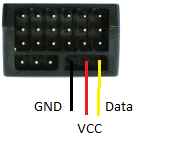
\includegraphics{fig_motor/GR-16.png}
	\caption[GR-16 Verkabelung]{GR-16 Verkabelung\protect\footnotemark}
\end{figure}
\footnotetext{http://www.graupner.de/mediaroot/files/33508\_Kurzanleitung\_de.pdf}
Die Spannung und Ground kann direkt �ber das Raspberry Pi bezogen werden. F�r die Daten muss einer der GPIO Pins als Input deklariert werden.

Um die Fernbedienung mx-20 mit dem Empf�nger GR-16 zu verbinden m�ssen beide Ger�te eingeschaltet sein (Empf�nger LED blinkt Rot). Beim Anschalten der Fernbedienung wird gefragt ob \emph{HF} EIN oder AUS ist. Stellen Sie auf AUS und best�tigen Sie mit Dr�cken der Set-Taste. Dr�cken sie erneut Set um in die Einstellungen zu gelangen. Scrollen Sie sich mit den Pfeiltasten durch das Men� bis Sie das Men� \emph{Grundeinstellungen Mod.} sehen. �ffnen Sie mit Set das Men� und scrollen Sie durch bis zu Punkt \emph{Modul}. Best�tigen Sie noch NICHT mit der Set-Taste. 
Halten Sie nun am Empf�nger solange die Set Taste gedr�ckt, bis sich zur der roten LED noch eine gr�ne LED einschaltet. Bet�tigen Sie jetzt den Set-Taster auf der Fernbedienung. Es sollte der Info-Text \emph{Binden ...} angezeigt werden.
Wenn die Verbindung erfolgreich durchgef�hrt wurde leuchtet die LED dauerhaft gr�n. \cite{doc:gt-16}

\newpage

\section{Debuggen der Programme}

\paragraph{Target laden}
Rechtsklick auf Projekt Ordner, \newline
Build Configurations -> Set Active -> Target.\newline
Rechtsklick auf Projekt Ordner, Build Project.

Debug Pfeil anklicken und helicopter-raspberry target ausw�hlen.

Oder �ber das Terminal: In das Verzeichnis \emph{helikopter-raspberry/impl/trunk/} wechseln
und mit dem Befehl \newline
\emph{make MAKECMDGOALS=target}\newline
das Programm  kompilieren und automatisch auf das Raspberry Pi laden.

\paragraph{Host laden}
Rechtsklick auf Projekt Ordner, 
Build Configurations -> Set Active -> Host.
Rechtsklick auf Projekt Ordner, Build Project.

Debug Pfeil anklicken und READ-UDP ausw�hlen.

\paragraph{Programme laufen lassen}
In die Debug-Ansicht von Eclipse wechseln (oben rechts). In dem Debug-Fenster sollten nun eine Remote-Anwendung (Anwendung auf Pi) und eine Host-Anwendung gestartet sein. Um diese laufen zu lassen muss der jeweilige Prozess ausgew�hlt werden und auf Resume geklickt werden sowie ggf. Breakpoints entfernt werden.

Nachdem die beiden Programme laufen muss noch der zu startende Testfall ausgew�hlt werden. Dies geschieht, in dem man �ber die Console die jeweiligen Testfall ausw�hlt, z.B. "testmatlabimu". Das im Grundlagenteil Udp-Programm ist hier als Testfall eingef�gt und kann mit der Eingabe "testudp" gestartet werden.

Nun laufen die Programme. Falls im ausgew�hlten Testfall Ausgaben vorhanden sind, sind diese in der Console zu sehen.

\paragraph{Beenden der Applicationen}
Um Probleme zu vermeiden ist es wichtig, die laufenden Programme immer manuell anzuhalten und zu \emph{killen}. Dies gelingt, in dem man in der Debug-Ansicht auf das zu beendene Programm rechtsklickt und auf Terminate klickt. 

\paragraph{Testf�lle}
In der main.c wird in dem definiertem \emph{enum} enumTestCases ein neuer Testfall angelegt.
In der int main(){...} wird bei Start auf eine Eingabe des zu startenden Testfalles gewartet. Hier muss noch ein \emph{else if}-Anweisung erg�nzt werden. 
In der Variable runCommand wird der Name des abzuarbeitenden Testfalles abgespeichert.
In der nachfolgenden \emph{Switch}-Anweisung steht der eigentliche Code, welcher bei Auswahl dieses Testfalles ausgef�hrt wird.

\newpage
\section{Umstellung auf eine automatische dynamische Testumgebung}

Die Main-Funktion zum Testen soll umstrukturiert werden, da die vorherige Struktur recht umst�ndlich zu testen und zu bedienen war. Es muss vor jedem einzelnen Testfall das Programm komplett auf das Raspberry �bertragen werden und �ber die Remote-Verbindung der zu startende Testfall h�ndisch ausgew�hlt werden. Dieser wird ausgef�hrt und das Programm ist beendet, sobald der Testfall beendet ist. Um einen weiteren Test zu starten musste wieder eine Remote-Verbindung aufgebaut werden. Dies funktioniert, ist aber nicht die optimale L�sung.

Stattdessen soll die neue Main-Funktion �ber eine Dauerschleife verf�gen, in dieser ein Textfile ausgelesen wird. Dieses File beinhaltet die zu startenden Testcases des Programmes.

In diesem Textfile werden alle Testf�lle festgehalten, mit einem Status ob dieser laufen soll oder nicht. Der Status soll w�hrend der Laufzeit des Programmes �nderbar sein und dieses auch nicht unterbrechen.

Dieses Textfile sieht folgenderma�en aus:

...\\
testmotorpwm=1\\
testmotorisr=1\\
testmotortxt=0\\
....\\

Dies bedeutet: die Testf�lle testmotorpwm und testmotorisr sollen gestartet werden, testmotortxt soll nicht gestartet werden.
Der Testfall testmotorpwm wird zuerst ausgelesen und von der Main-Funktion auf Null zur�ckgesetzt. Anschlie�end l�uft der Testfall ab.

W�hrenddessen wird der Testfall testmotortxt aktiviert. 

...\\
testmotorpwm=0\\
testmotorisr=1\\
testmotortxt=1\\
....

Ist der Testfall beendet wird das Textfile erneut eingelesen und der n�chste gesetzte Testfall wird gestartet.

\newpage
\paragraph{Umstrukturierung der main.c:}

Es wurde eine Endlosschleife eingef�gt. Statt auf eine Tastatureingabe �ber eine Konsole zu warten, wird in dieser alle zwei Sekunden das \textit{\_Testfile} ausgelesen und �berpr�ft, ob ein Testfall ausgef�hrt werden soll.


In allen Testf�llen darf keine Endlosschleife vorhanden sein, bzw. muss in weiteren Endlosschleifen ein Abbruchkriterium festgelegt sein. In den meisten F�llen kann der Testfall mit Dr�cken der Taste \textit{p} abgebrochen werden. In Testf�llen, in denen ein Testfile ausgelesen wird, wird bei Erreichen des Dateiendes der Testfall beendet und gelangt so wieder in die Hauptschleife zur�ck.

\paragraph{Script zum Setzen der Testf�lle:}

Zum Setzen oder L�schen eines Testfiles wurde ein Script geschrieben, welches auf das textfile \textit{\_Testfile} zugreift und die Eintr�ge je nach Eingabe �berarbeitet.

Verwendet wird das Script folgenderma�en:

\begin{lstlisting}[language=bash]
.\testcase NameTestfall [Modus]
\end{lstlisting}
 	 
Als ersten Parameter ist der zu �berarbeitende Testfall anzugeben.\\
Der Modus ist ein optionaler Parameter. Ist dieser Parameter nicht vorhanden, wird automatisch \emph{set} angenommen. \textit{set} markiert den Testfall als abzuarbeiten, \textit{clear} l�scht diese Markierung wiederrum. Das Script zeigt keinen Fehler oder Warnung auf, wenn der testcase nicht gelistet ist.

Der Quellcode ist im Kapitel \ref{script_testcase} \nameref{script_testcase} auf S.\pageref{script_testcase} einzusehen.

\newpage
\section{Valedierung der empfangenen Werte}
\label{sec:real-unter}
Im testcase testmatlabimu stimmen die empfangenen und gesendeten Werte nicht �berein. Hier ist der Fehler zu finden und zu beheben.

Es werden insgesamt 11 double Values von den diversen Sensoren an den Host gesendet. Die Kalkulation der Werte ist richtig, kommen jedoch beim Empf�nger falsch an. Dieses Fehlverhalten gilt es zu untersuchen.

Hierf�r wurde ein neuer Testfall angelegt, alle 11 Double Werte per UDP versendet und diese auf beiden Seiten ausgegeben. 

Nach dem Setzen der Breakpoints, so das nur einmal die Werte gesendet werden, erhalten wir folgende Ausgaben auf der Console:

\begin{multicols}{2}
	 \begin{lstlisting}[language=C++]
	 Starting read over UDP
	 /home/ezs/git/helikopter- raspberry/impl/trunk/host /READ-UDP.elf: Wartet auf Daten am Port (UDP) 5000
	 Acc X 0.000000 
	 Acc Y 0.910135 
	 Acc Z -0.488599 
	 Mag X -10.533617 
	 Mag Y 0.000024 
	 Mag Z 0.000021 
	 Gyro yaw 0.000014 
	 Gyro pitch -0.473037 nGyro roll 0.473037 
	 Temp -0.396741 
	 Press 31.825000 
	 \end{lstlisting}
	
	\columnbreak
	
	 \begin{lstlisting}[language=C++]
	 Received string is testallsensordata 
	 Starting IMU Matlab Test
	 
	 
	 Acc X 0.910135 
	 Acc Y -0.488599 
	 Acc Z -10.533617 
	 Mag X 0.000024 
	 Mag Y 0.000021 
	 Mag Z 0.000014 
	 Gyro yaw -0.473037 
	 Gyro pitch 0.473037 
	 Gyro roll -0.396741 
	 Temp 31.825000 
	 Press 987.931396 
	 \end{lstlisting}
\end{multicols}
 

Nach einem Vergleich f�llt auf, dass beim Empfang der Daten sich bei X-Wert vom Acc eine Null eingef�gt hat. Ansonsten scheinen die Daten zu stimmen. Die Daten sind nur um eins versetzt.

In der read-udp-host.c werden die Werte in der Variable \emph{l\_recvImuState\_st} gespeichert. Beim Betrachten der Inhalte dieser Variablen ist zu erkennen, dass diese in \emph{acc.f64} einen Wert hat der Circa null entspricht, die restlichen Werte sehen richtig aus, nur weiterhin um einen Wert verschoben.

Verdacht: Beim Senden der Daten wird auch noch ein Zeitstempel dieses Telegramms mitgesendet: 
\begin{lstlisting}[language=C++]
//time.h
struct timespec{
	__time_t tv_sec; /* Seconds */
	__syscall_slong_t tv_ns	/* Seconds */
	};

//udpImuLib.c
struct timespec l_timespec_st;

\end{lstlisting}

Diese Daten haben die L�nge von 8 Byte (beide vom Typ long int). Diese Daten werden mit den Sensordaten gesendet. Die Paketl�nge nimmt zu.
Da auf der Empf�ngerseite die Empfangsstruktur aber diesen timestamp nicht erwartet, geht er davon aus, dass der erste Wert, den er bekommt, f�r den Acc X Sensor-Wert steht.
Aus diesem Grund verrutschen die restlichen Daten um eins ab und der erste Sensor-Wert ist falsch da dieser den Timestamp widerspiegelt.

\paragraph{Problembehebung}
Die fehlenden Daten m�ssen in dem Struct bekannt gemacht werden, sodass die L�nge der beiden Felder nun gleich Gro� sind (96 Byte).
Hierf�r musste das Struct \emph{halImu\_orientationValues} im imu.h um einen Datentyp struct timespec erweitert werden sowie die notwendige Standardlibary \emph{time.h} hinzugef�gt werden.
Dann wurde die Testausgabe um den Timestamp erweitert.
Die Werte stimmen nun �berein:
\begin{multicols}{2}
	\begin{lstlisting}[language=C++]
	Starting read over UDP
	/home/ezs/git/helikopter -raspberry/impl/trunk/host /READ-UDP.elf: Wartet auf Daten am Port (UDP) 5000
	Time  1434105267.000000000 
	Acc X 0.792776 
	Acc Y -0.555661 
	Acc Z -10.581519 
	Mag X 0.000024 
	Mag Y 0.000021 
	Mag Z 0.000014 
	Gyro yaw -0.228889 
	Gyro pitch -0.122074 
	Gyro roll -0.488296 
	Temp 32.056250 
	Press 987.923828 
	\end{lstlisting}
	\columnbreak
	\begin{lstlisting}[language=C++]
	 Received string is testallsensordata 
		Starting IMU Matlab Test
		 
	
	
	Acc X 0.792776 
	Acc Y -0.555661 
	Acc Z -10.581519 
	Mag X 0.000024 
	Mag Y 0.000021 
	Mag Z 0.000014 
	Gyro yaw -0.228889 
	Gyro pitch -0.122074 
	Gyro roll -0.488296 
	Temp 32.056250 
	Press 987.923828 
	\end{lstlisting}
\end{multicols}

\begin{lstlisting}[language=C++]
#include <time.h>
typedef struct{
	struct timespec l_timestamp_st;
	halAccmag_3dDoubleVector acc;
	halAccmag_3dDoubleVector mag;
	strGyro gyro;
	double temperature_f64;
	double pressure_f64;
} halImu_orientationValues;

\end{lstlisting}

\section{Software Motortreiber}

Es soll Software f�r den Hardware-Treiber, der die Motoren ansteuert, geschrieben werden. Zun�chst muss der Raspberry Pi mit dem I2C-Bus verbunden werden. 
Die I2C Adressen der Motoren sind in der Motor.h hinterlegt. F�r die Quadrocopter wurden die Werte definiert. Die Werte des Octocopter m�ssen zun�chst �berpr�ft werden.

Mittels des Befehl:

\begin{center}
	i2cdetect -y 1
\end{center}

k�nnen die vergebenen Adressen im Bussystem angezeigt und validiert werden.

Die Daten, die von dem Hardware Brushless-Controller erwartet werden, besitzen folgendes Format:

	\begin{table}[H]
		\centering
		\begin{tabular}{|c|c|}
			\hline
			I2C Adresse [1 Byte] & PWM Value [1 Byte]\\ \hline
		\end{tabular}
	\caption{I2C Frame Brushless Motoren Treiber}
	\end{table}

Mit Hilfe des Befehls 

\begin{center}
	i2cset -y 1 0x29 0x55
\end{center}

wird an den Controller mit der I2C Adresse 0x29 ( Motor Nr.1) der Wert 0x55 gesendet.

\subsection{Verwendung des Software-Treibers}

In der main.h muss zun�chst definiert werden, auf welchem Typ von den HElicoptern das Programm geladen werden soll.
\begin{lstlisting}[language=C++]
#include <time.h>
#define Quadro_Plus 1
//#define Quadro_X 1
//#define Okto_Plus 1
\end{lstlisting}

Anschlie�end sollte baldm�glichst die InitMotor() aufgerufen werden, die unter anderem einen Timer initialisiert und startet. Bei Ablauf des Timers wird ein Flag gesetzt. Dieses Flag muss im Quellcode mit der Funktion \emph{GetFlagRunSendPwmToMotor()} abgefragt werden. Wenn dieses Flag gesetzt ist, muss die Funktion \emph{sendPwmToMotor()} aufgerufen werden.

\begin{lstlisting}[language=C++]
...
InitMotor();
...
while(1){
...
if(GetFlagRunSendPwmToMotor() == 1){
sendPwmToMotor();
}
...

}
\end{lstlisting}
Der aktuelle PWM-Wert eines Motors kann mittels der Funktion \emph{GetPwmMotor(...)} zur�ckgegeben werden.

\begin{lstlisting}[language=C++]
value = GetPwmMotor(6);
value > 0? value--: (value=DEFMotorSetpointMIN);
SetPwmMotor(DEFMotorNo7_PWM, value ,0);
\end{lstlisting}

Wichtig: Alle ISR sollen knapp gehalten werden, da ansonsten die Motoren nicht mehr angesprochen werden k�nnen.

Mit der Funktion \emph{SetPwmMotor(...)} k�nnen die PWM-Werte, die  per I2C gesendet werden, �berschrieben werden. Optional kann ein Flag gesetzt werden. Ist dies der Fall wird anschlie�end die Funktion \emph{sendPwmToMotor()} aufgerufen.

\subsection{Headerfile}

Hier sind die verschiedenen HElicopter Varianten sowie deren definierte Eigenschaften (Anzahl Motoren, Drehrichtung der Motoren, Motorenreihenfogen) festgehalten.

F�r weitere Informationen (wie z.B. Namen der defines) siehe in Kapitel \ref{motorH} in  \nameref{motorH} auf S.\pageref{motorH} .

\subsection{Funktionen}

Beschreibung der Funktionen befinden sich in den jeweiligen dar�ber liegenden Kommentaren mit Parametern und Return Values.

Auf alle globalen Variablen/Flags werden mit Funktionen zugegriffen. Ein direkter Zugriff ist zu vermeiden.

\begin{lstlisting}[language=C++,firstnumber=14]
/* Global Variables */
char BLCtrlADRExecuteOrder[DEFMotorsCount];
char PWMValue[DEFMotorsCount];

//Flags
char flagRunSendPwmToMotor;
\end{lstlisting}

\begin{lstlisting}[language=C++,firstnumber=21]
/*!***************************************************************
* \author Chris Mönch( chmoit00 )
*
* \brief calls init functions which needed for the motor driver:
* SetFlagRunSendPwmToMotor(0);
*	SetMotorExecutionOrder();
*	SetPwmMotor(DEFMotorALL_PWM, DEFMotorSetpointMIN, 0);
*	Last one always initMotorTimer()
*	InitMotorTimer(microSeconds);
*	SetFlagRunSendPwmToMotor(1);
*
* \param[ in ] microSeconds - Time in uS when Timer expired.
*
* \internal
* CHANGELOG:
*
* \endinternal
*****************************************************************/
void InitMotor(int microSeconds){
	SetFlagRunSendPwmToMotor(0);
	SetMotorExecutionOrder();
	SetPwmMotor(DEFMotorALL_PWM, DEFMotorSetpointMIN, 0);
	//Last one always initMotorTimer()
	InitMotorTimer(microSeconds);
	SetFlagRunSendPwmToMotor(1);
}
\end{lstlisting}

\begin{lstlisting}[language=C++,firstnumber=48]
/*!***************************************************************
* \author Chris Mönch( chmoit00 )
* \date 2016/01/08
*
* \brief set Motor Exectution Order
*
* \internal
* CHANGELOG:
*
* \endinternal
*****************************************************************/
void SetMotorExecutionOrder(){
	GetBLCtrlADRExecuteOrder(&BLCtrlADRExecuteOrder[0]);
}
\end{lstlisting}

\begin{lstlisting}[language=C++,firstnumber=63]
/*!***************************************************************
* \author Chris Mönch( chmoit00 )
* \date 2016/01/08
*
* \brief sets PWM Signal of selected Motor to pwmValue
* \details toSet = 00001111 sets the first 4 Motors in Execution Order to pwmValue
*
* \param[ in ] toSet - Which Motor to Set
* \param[ in ] pwmValue - Which Value so Set
* \param[ in ] forceSend - optional Parameter if !0 flagRunSendPwmToMotor will be set
*
* \internal
* CHANGELOG:
*
* \endinternal
*****************************************************************/
void SetPwmMotor(char toSet , int pwmValue, int forceSend){
	int i=0;
	pwmValue = pwmValue >= DEFMotorSetpointMIN ? pwmValue :  DEFMotorSetpointMIN;
	pwmValue = pwmValue <= DEFMotorSetpointMAX ?  pwmValue :  DEFMotorSetpointMAX;
	while(toSet != 0 && i < DEFMotorsCount){
	
		if(toSet%2){
			PWMValue[i]= pwmValue;
		}
		toSet= toSet >>1;
		i++;
	}
	if(forceSend != 0){
		SetFlagRunSendPwmToMotor(1);
	}
}
\end{lstlisting}

\begin{lstlisting}[language=C++,firstnumber=96]
/*!***************************************************************
* \author Chris Mönch( chmoit00 )
* \date 2016/01/08
*
* \brief adds to the current PWM Signal of selected Motor the pwmValue
* \details toSet = 00001111 add to the first 4 motors pwmValue
*
* \param[ in ] toSet - Which Motor to Set
* \param[ in ] pwmValue - adding pwm value to current PWMValue
* \param[ in ] forceSend - optional Parameter if !0 flagRunSendPwmToMotor will be set
*
* \internal
* CHANGELOG:
*
* \endinternal
*****************************************************************/
void AddPwmMotor(char toSet , int pwmValue, int forceSend){
	int i=0;
	
	while(toSet != 0 && i < DEFMotorsCount){
	
		if(toSet%2){
			pwmValue = pwmValue+GetPwmMotor(i);
			pwmValue = pwmValue >= DEFMotorSetpointMIN ? pwmValue :  DEFMotorSetpointMIN;
			pwmValue = pwmValue <= DEFMotorSetpointMAX ?  pwmValue :  DEFMotorSetpointMAX;
			PWMValue[i]= pwmValue;
		}
		toSet= toSet >>1;
		i++;
	}
	if(forceSend != 0){
		SetFlagRunSendPwmToMotor(1);
	}
}

\end{lstlisting}

\begin{lstlisting}[language=C++,firstnumber=131]
/*!***************************************************************
* \author Chris Mönch( chmoit00 )
* \date 2016/01/08
*
* \brief Subtract to the current PWM Signal of selected Motor the pwmValue
* \details toSet = 00001111 subtract to the first 4 motors pwmValue
*
* \param[ in ] toSet - Which Motor to Set
* \param[ in ] pwmValue - pwm value to subtract from Current PWMValue
* \param[ in ] forceSend - optional Parameter if !0 flagRunSendPwmToMotor will be set
*
* \internal
* CHANGELOG:
*
* \endinternal
*****************************************************************/
void SubbPwmMotor(char toSet , int pwmValue, int forceSend){
	int i=0;
	
	while(toSet != 0 && i < DEFMotorsCount){
	
		if(toSet%2){
			pwmValue = GetPwmMotor(i)- pwmValue;
			pwmValue = pwmValue >= DEFMotorSetpointMIN ? pwmValue :  DEFMotorSetpointMIN;
			pwmValue = pwmValue <= DEFMotorSetpointMAX ?  pwmValue :  DEFMotorSetpointMAX;
			PWMValue[i]= pwmValue;
		}
		toSet= toSet >>1;
		i++;
		}
	if(forceSend != 0){
		SetFlagRunSendPwmToMotor(1);
	}
}
\end{lstlisting}

\begin{lstlisting}[language=C++,firstnumber=167]
/*!***************************************************************
* \author Chris Mönch( chmoit00 )
* \date 2016/01/08
*
* \brief Gets pwmValue from a specific motor
* \details
*
* \param[ in ] motorNumber - which motor
*
* \param[ out ] pwmValue of the chosen Motor, returns O if chosen Motor not exist in these HElicoptertype
* 
* \internal
* CHANGELOG:
*
* \endinternal
*****************************************************************/
int GetPwmMotor(int motorNumber){
	return motorNumber < DEFMotorsCount ? PWMValue[motorNumber]: 0;
}
\end{lstlisting}

\begin{lstlisting}[language=C++,firstnumber=188]
/*!***************************************************************
* \author Chris Mönch( chmoit00 )
* \date 2016/01/08
*
* \brief init Timer for the IsrMotor
* \details
*
* \param[ in ] microSeconds - Time in uS when Timer expired.
*
* \internal
* CHANGELOG:
*
* \endinternal
*****************************************************************/
void InitMotorTimer(int microSeconds){

	struct sigaction sa;
	struct itimerval timer;
	
	//Creates Signal, if signal Rising a_handler called
	memset(&sa, 0 , sizeof(sa));
	sa.sa_handler = &IsrSetFlag;
	sigaction(SIGVTALRM, &sa, NULL);
	
	//Expire the Timer after:
	timer.it_value.tv_sec = 0;
	timer.it_value.tv_usec = 0;
	//And every ... after that:
	timer.it_interval.tv_sec = 0;
	timer.it_interval.tv_usec = microSeconds;
	//upon expiration the signal SIGVTALRM raised
	setitimer(ITIMER_VIRTUAL, &timer , NULL);
}
\end{lstlisting}

\begin{lstlisting}[language=C++,firstnumber=222]
/*!***************************************************************
* \author Chris Mönch( chmoit00 )
* \date 2016/01/08
*
* \brief set flag flagRunSendPwmToMotor
*
* \param[ in ] 1 Set Flag, else clear Flag
*
* \internal
* CHANGELOG:
*
* \endinternal
*****************************************************************/
void SetFlagRunSendPwmToMotor(char value){
	if(value == 1){
		flagRunSendPwmToMotor=value;
	}else{
		flagRunSendPwmToMotor=0;
	}
}
\end{lstlisting}

\begin{lstlisting}[language=C++,firstnumber=243]
/*!***************************************************************
* \author Chris Mönch( chmoit00 )
* \date 2016/01/08
*
* \brief ISR for set flag as flagRunSendPwmToMotor
*
* \internal
* CHANGELOG:
*
* \endinternal
*****************************************************************/
void IsrSetFlag(){
	flagRunSendPwmToMotor=1;
}
\end{lstlisting}

\begin{lstlisting}[language=C++,firstnumber=258]
/*!***************************************************************
* \author Chris Mönch( chmoit00 )
* \date 2016/01/08
*
* \brief get flag flagRunSendPwmToMotor
*
* \param[out] flag flagRunSendPwmToMotor
*
* \internal
* CHANGELOG:
*
* \endinternal
*****************************************************************/
char GetFlagRunSendPwmToMotor(){
	return flagRunSendPwmToMotor;
}
\end{lstlisting}

\begin{lstlisting}[language=C++,firstnumber=275]
/*!***************************************************************
* \author Chris Mönch( chmoit00 )
* \date 2016/01/08
*
* \brief sends every timer interrupt to the motors the specific pwm values
*
* \internal
* CHANGELOG:
*
* \endinternal
*****************************************************************/
void sendPwmToMotor(){
	int i;
	for(i = 0; i < DEFMotorsCount ;i++)
	{
		g_lldI2c_WriteI2c_bl(BLCtrlADRExecuteOrder[i],&PWMValue[i],1);
	}
}
\end{lstlisting}

\begin{lstlisting}[language=C++,firstnumber=294]
/*!***************************************************************
* \author Chris Mönch( chmoit00 )
* \date 2016/01/08
*
* \brief Get the I2C addresses orderd by execution (defined in MOTOR.h)
* \details
*
* \param[ in ] Array where the I2C Addresses will be stored
*
* \internal
* CHANGELOG:
*
* \endinternal
*****************************************************************/
void GetBLCtrlADRExecuteOrder(char BLCtrlADRExecuteOrder[]){
#if defined(Quadro_X) || defined(Quadro_Plus)
int BLCTRLADR[4] = {DEFMotorNo1_BLCtrlADR, DEFMotorNo2_BLCtrlADR, DEFMotorNo3_BLCtrlADR, DEFMotorNo4_BLCtrlADR};

BLCtrlADRExecuteOrder[DEFMotorNo1_OrderIDX ]=BLCTRLADR[0];
BLCtrlADRExecuteOrder[DEFMotorNo2_OrderIDX]=BLCTRLADR[1];
BLCtrlADRExecuteOrder[DEFMotorNo3_OrderIDX]=BLCTRLADR[2];
BLCtrlADRExecuteOrder[DEFMotorNo4_OrderIDX]=BLCTRLADR[3];

#endif

#ifdef Okto_Plus
int BLCTRLADR[8] = {DEFMotorNo1_BLCtrlADR, DEFMotorNo2_BLCtrlADR, DEFMotorNo3_BLCtrlADR
DEFMotorNo4_BLCtrlADR, DEFMotorNo5_BLCtrlADR, DEFMotorNo6_BLCtrlADR,
DEFMotorNo7_BLCtrlADR, DEFMotorNo8_BLCtrlADR};

BLCtrlADRExecuteOrder[DEFMotorNo1_OrderIDX]=BLCTRLADR[0];
BLCtrlADRExecuteOrder[DEFMotorNo2_OrderIDX]=BLCTRLADR[1];
BLCtrlADRExecuteOrder[DEFMotorNo3_OrderIDX]=BLCTRLADR[2];
BLCtrlADRExecuteOrder[DEFMotorNo4_OrderIDX]=BLCTRLADR[3];
BLCtrlADRExecuteOrder[DEFMotorNo5_OrderIDX]=BLCTRLADR[4];
BLCtrlADRExecuteOrder[DEFMotorNo6_OrderIDX]=BLCTRLADR[5];
BLCtrlADRExecuteOrder[DEFMotorNo7_OrderIDX]=BLCTRLADR[6];
BLCtrlADRExecuteOrder[DEFMotorNo8_OrderIDX]=BLCTRLADR[7];

#endif
}
\end{lstlisting}

\subsection{Testf�lle}

Um die Funktionalit�t des Treiber zu testen und kontrollieren sind die folgenden Testf�lle geschrieben worden. 

\subparagraph{TESTMOTORPWM}

Dieses Testprogramm sendet alle 10ms an die Motoren einen stets steigenden PWM-Wert bis zum Wert 0x50. Bei erreichen des Wertes wird der PWM-Wert auf den definiertes Minimum gesetzt. Dieser Testfall l�uft ohne ISR ab. Die Daten werden direkt �ber I2C gesendet. Die Schrittweite und das Maximum des Testfalles sind per Konstanten definiert und k�nnen ver�ndert werden. 

\subparagraph{TESTMOTORISR}

Mit diesem Testprogramm wird die ISR-Funktion getestet. Durch Eingabe in der Konsole wie z.B.

+0+0+0+0+7+7+7-8

wird der  PWM-Wert des Motors 0 um vier erh�ht, der Motor 7 um drei erh�ht und der Motor 8 um eins verringert. Die Eingabe ist nicht blockierend. Zum Starten des Testfalls muss ein '+' eingetippt werden.

\subparagraph{TESTMOTORTXT}

Der letzte Testfall liest aus einem Textfile, das sich auf dem Raspberry unter dem Pfad \emph{/home/pi/MotorTest.txt} befinden muss, Zeile f�r Zeile aus und setzt die PWM-Werte so, wie sie in der Zeile angegeben sind.

Die Befehlszeile hat folgendes Format:
\newline
\begin{center}
\#MOTORNUMER[+][-][=][PWMWERT]\;DELAY
\end{center}
z.B.
\#0+100;10 \t - \t Der PWM des Motors 0 erh�ht sich um 100. Die n�chste Zeile wird in 10s eingelesen.
\newpage
\section{Help Functions}

\paragraph{Nicht blockierende Eingabe Funktion kbhit}
Diverse Testf�lle h�ngen von einer Tastatur Eingabe ab. Die Standardfunktionen hierf�r sind blockierende Funktionen. Diese d�rfen jedoch nicht verwendet werden, da die Motoren nicht angesteuert werden k�nnen.
Um Tastatureingaben m�glich zu machen, wurde eine Funktion geschrieben, die den Programmablauf nicht blockiert. Als Return-Wert gibt es immer die zuletzt gedr�ckte Taste zur�ck.

Eine Eingabe, die aus mehreren Chars, besteht muss mit mehreren \emph{kbhit()} aufrufen und durch Schleifen oder if-Verzweigung �berpr�ft werden. Die Eingabe wird aus dem Buffer gelesen.


\begin{lstlisting}[language=C++,firstnumber=0]
#include <termios.h>

int kbhit(void)
{
	struct termios term, oterm;
	int fd = 0;
	int c = 0;
	tcgetattr(fd, &oterm);
	memcpy(&term, &oterm, sizeof(term));
	term.c_lflag = term.c_lflag & (!ICANON);
	term.c_cc[VMIN] = 0;
	term.c_cc[VTIME] = 1;
	tcsetattr(fd, TCSANOW, &term);
	c = getchar();
	tcsetattr(fd, TCSANOW, &oterm);
	return c; 
}
\end{lstlisting}
\newpage
\section{Remotecontroller-Treiber}
\label{Controller Treiber}

Um den autonomen Start bzw. Landevorgang des Quadrocopter einzuleiten muss eine Funkverbindung �ber eine Fernbedienung und einen Transmitter eingerichtet werden. Die Daten sind anschlie�end auszuwerten und zu verarbeiten.

Als Fernbedienung von der Firma Graupner dient der \emph{MX-20} und als Receiver der \emph{GR-16}. Der Anschluss des Receivers erfolgt �ber drei Leitungen:
\begin{itemize} 
	\item  Versorgungsspannung:  5Volt (vom Raspberry) 
	\item  Ground (Raspberry)
	\item PPM (Puls-Pause Modulation) (auf einen der GPIO Pins)
\end{itemize}


\paragraph{Verbinden mit Receiver}
Schalten Sie die Fernbedienung ein und schlie�en den Receiver an den Raspberry Pi an [siehe Abschnitt~ \ref{Receiver} auf Seite \pageref{Receiver}]

\paragraph{PPM-Signal} genannt Puls-Pausen-Modulation (oder auch Puls-Position-Modulation) ist ein f�r analoge Werte verwendetes Kodierungsverfahren und wird vor allem in Funkfernsteuerungen verwendet. Der zu kodierende Wert wird in der L�nge des Pausen/Low Signals zwischen zwei Peaks/High Signalen gesendet. Diese Peaks haben stets die gleiche L�nge als auch gleiche Amplitude.\cite{doc:ppm}

Meist besteht ein PPM-Signal aus mehreren Kan�len zu einem Frame zusammengef�gt und  anschlie�end versendet.

F�r die Decodierung des PPM-Signals ist es empfehlen, ein weiteres Board zu integrieren, das die Decodierung  �bernimmt und die Ergebnisse an das Raspberry Pi weiterleitet, da das Signal sehr genau aufgel�st werden muss und die Decodierung �ber einen Interrupt gesteuert werden soll. Bei zu h�ufigen Auftreten des Interrupts w�rde der Helicopter destabilisiert werden. Zur Auswertung m�ssen nur die Raising Edges oder Falling Edges beachtet und der Offset des High-Pegels abgezogen werden.

Um auf ein weiteres Bauteil zu verzichten wurde stattdessen eine Real-Time-Linux-Version auf dem Raspberry Pi installiert, die die Signale im Nanosekundenbereich dekodieren kann.

\newpage
\paragraph{PPM Signal Mitschnitte}
Der Receiver sendet die empfangenen Signale im Format der Pulse-Pausen-Modulation. Mitgeschnittene �bertragungen\protect\footnotemark  mit Beschreibung sind beigef�gt.
\footnotetext{Von Herrn Trybek bereitgestellt}
\begin{figure}[H]
	\centering
	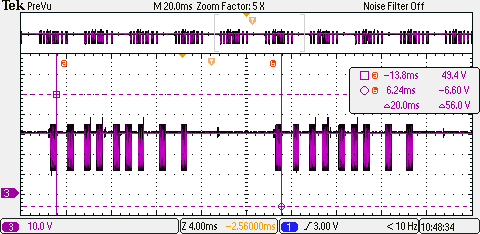
\includegraphics[width=0.6\textwidth]{fig_motor/Controller_Treiber/GraupnerGR16_8_Frame.png}
	\caption[8 Channel Frame]{8 Channel Frame}
\end{figure}

Es gibt zwei M�glichkeiten: ein Frame mit acht Kan�len, bestehend aus neun Peaks und acht Pausensignalen...

\begin{figure}[H]
	\centering
	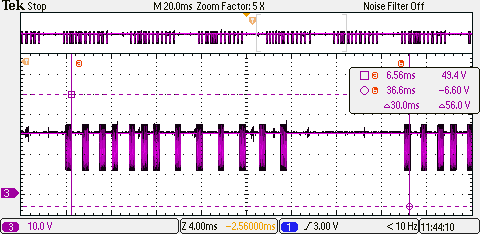
\includegraphics[width=0.6\textwidth]{fig_motor/Controller_Treiber/GraupnerGR16_12_Frame.png}
	\caption[12 Channel Frame]{12 Channel Frame}
\end{figure}

... oder einen 12 Kan�len Frame, bestehend aus 13 Peaks und 12 Pausensignalen.

\begin{figure}[H]
\centering
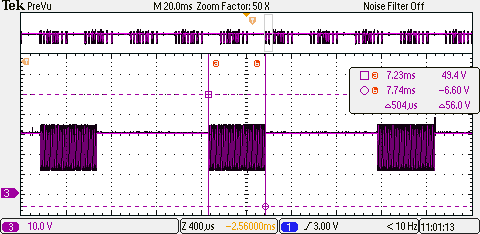
\includegraphics[width=0.6\textwidth]{fig_motor/Controller_Treiber/GraupnerGR16_8_ChX_Gap.png}
\caption[Dauer 8 chanel Frame ]{Dauer 8 Chanel Frame}
\end{figure}

Folgend die Anschaung eines Frames mit acht Kan�len mit der Dauer von 504us.

\begin{figure}[H]
	\centering
	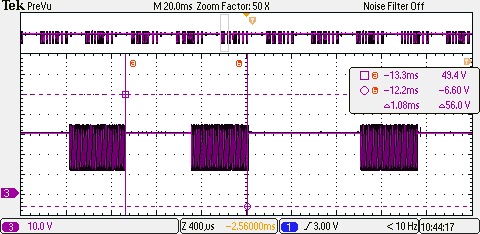
\includegraphics[width=0.6\textwidth]{fig_motor/Controller_Treiber/GraupnerGR16_8_Ch1_Min.png}
	\caption[Minimale Pause zwischen Frames]{Minimale Pause zwischen Frames}
\end{figure}

Zu sehen ist hier der kleinstm�gliche zeitliche Abstand zwischen zwei Frames mit der Dauer von nur 504us.

\begin{figure}[H]
	\centering
	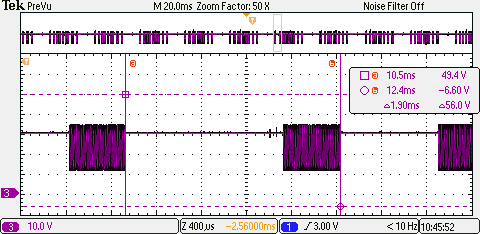
\includegraphics[width=0.6\textwidth]{fig_motor/Controller_Treiber/GraupnerGR16_8_Ch1_Max.png}
	\caption[Maximale Pause zwischen Frames]{Maximale Pause zwischen Frames}
\end{figure}

Hier ein Ausschnitt mit dem gr��tm�glichen Abstand zwischen zwei Frames mit der Dauer 1,396ms.

\section{Hardware Layout}
F�r die schnelle Durchf�hrung von �nderungen, Erweiterungen oder Anpassungen an der Hardware werden die Leiterplatinen und Schaltpl�ne mittels Tool elektronisch festgehalten. Die dazu m�gliche Software sind: EAGLE oder Fritzing,
die kostenlos oder als eingeschr�nkte Freeversion angeboten werden, aber diversen Einschr�nkungen unterliegen. Beide Tools haben eine Community, die viele Bauteile in Liberias bereitstellt. 

Im direktem Vergleich macht EAGLE einen professionelleren Eindruck und bietet eine Sammlung von Tutorials und Libraries. Aus diesen Gr�nden fiel die Entscheidung auf die EAGLE SOFTWARE. Es sollte aber mit dem Platz m�glichst sparend umgegangen werden, da bei dieser Freeeware die Gr��e und Anzahl der Layouts begrenzt ist.

\subsection{HElicopter Schematic Layout}

Es wurde f�r die schematischen Zeichnungen ein EAGLE Projekt angelegt, dass die schematischen Zeichnungen aller selbst gebauten bzw. zusammengef�gten Bauteile enth�lt. Das Projekt File ist im Verzeichnis \textit{trunk/hardware/} unter \textit{HElicopterPlus} abgespeichert.

Derzeit befinden sich zwei verschiedene schematischen Zeichnungen im Projektverzeichnis, die maximal aus zwei sogenannten Sheets besteht (Begrenzung durch die Freeware-Version von EAGLE). Der erster Sheet beinhaltet immer, denn Komplettaufbau des jeweiligen Systems. Der zweite Sheet wird verwendet um druckbare Versionen das Schaltplans zu erstellen (DINA4 Frame). Hierbei ist es wichtig, eine �bersichtliche Abspaltung vorzunehmen. 


\newpage
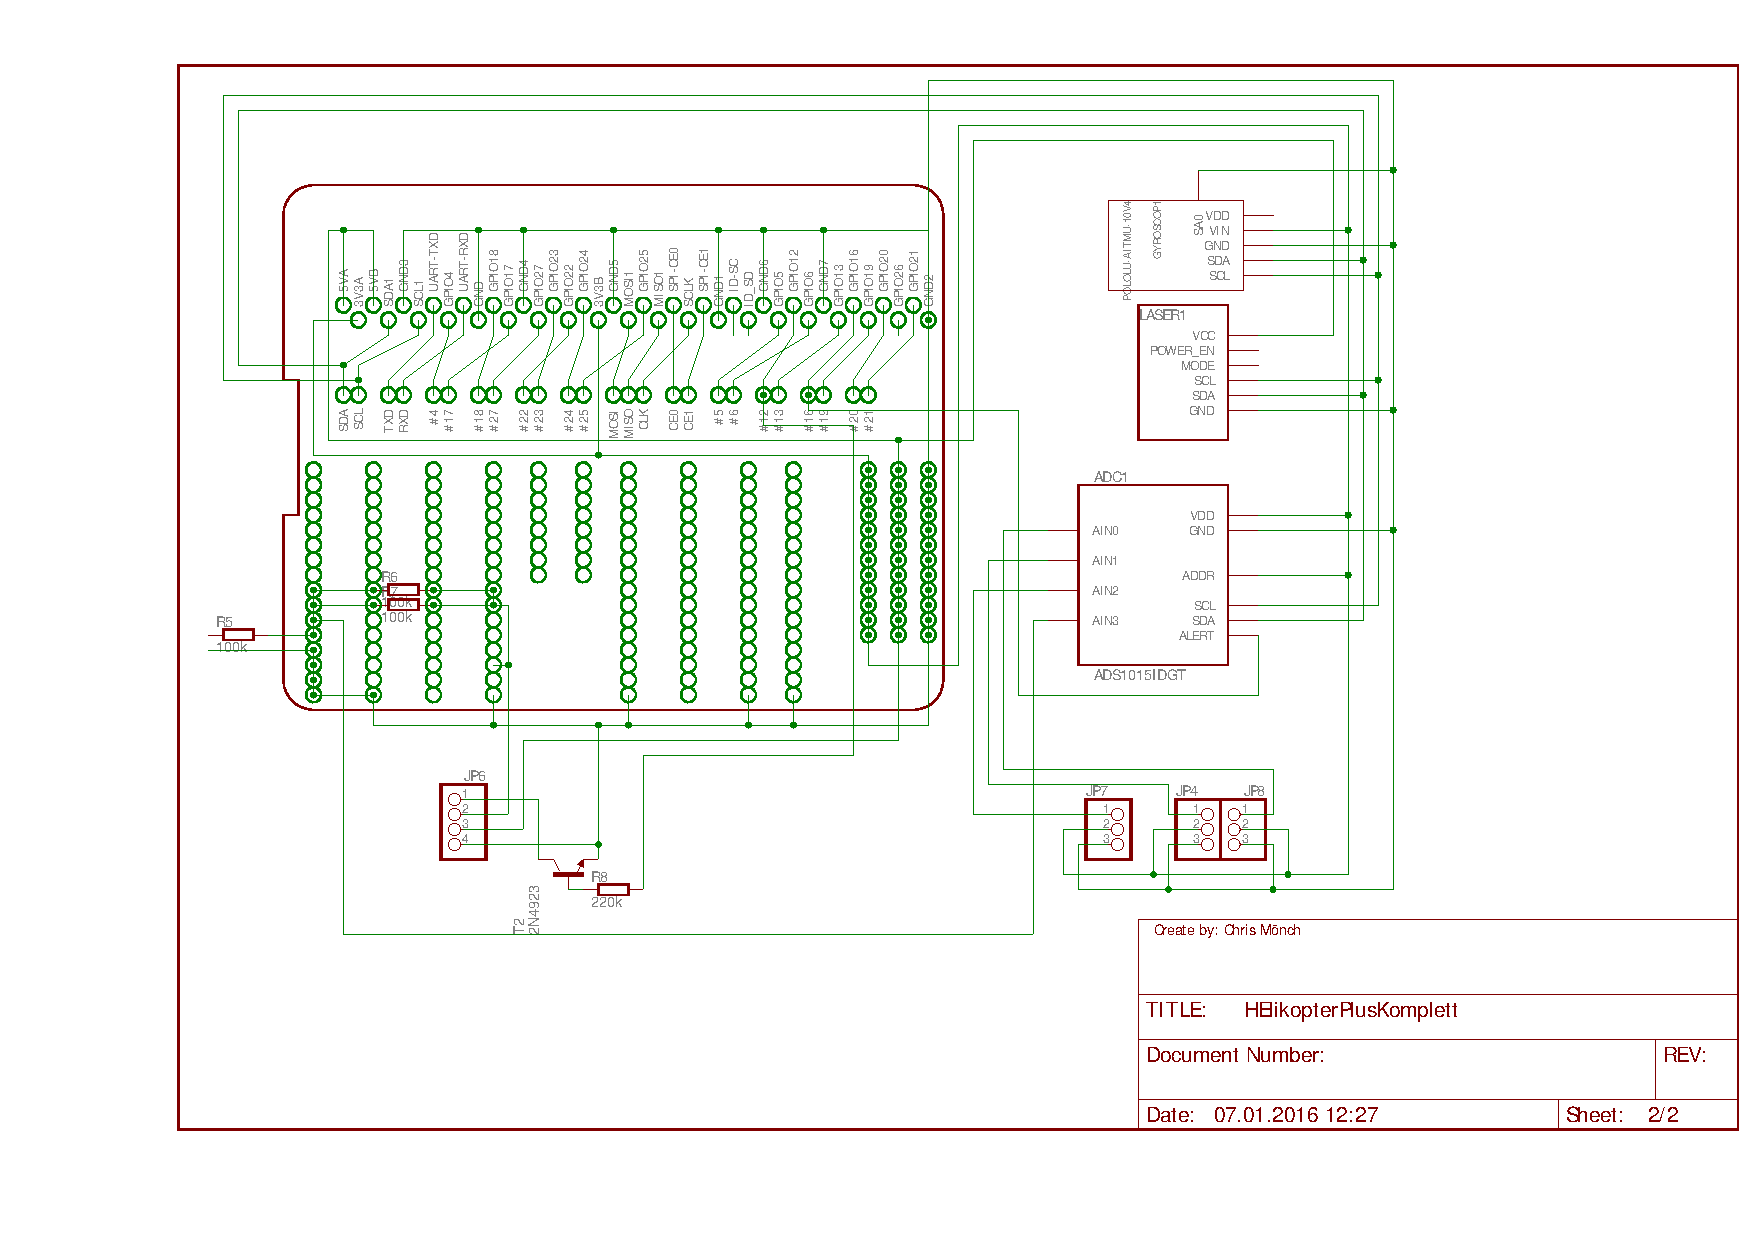
\includepdf[landscape=true,pages={1,2}]{fig_motor/Schematic/SchematicKomplettPrintVersion.pdf}
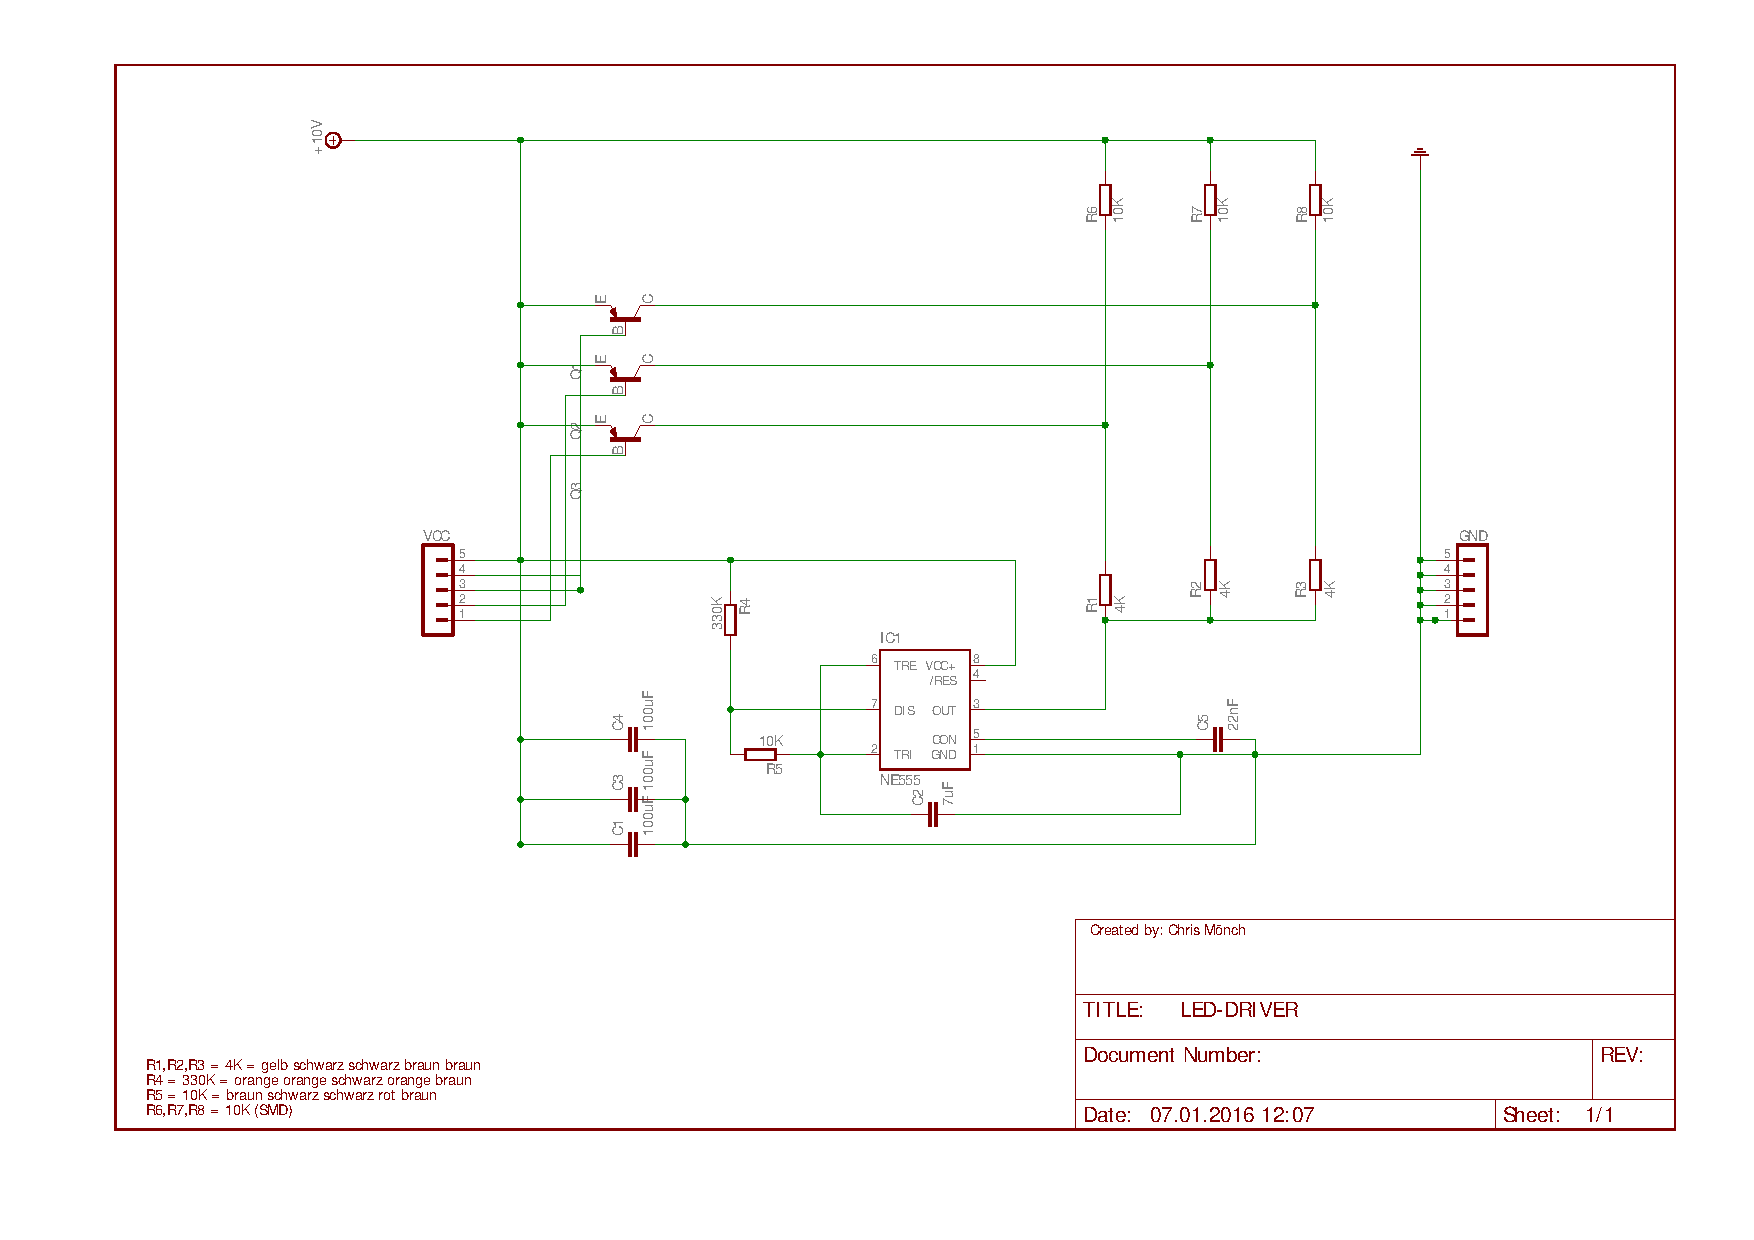
\includepdf[landscape=true]{fig_motor/Schematic/SchematicLedDriver.pdf}

\subsubsection{Richtlinien\cite{doc:guidelinesSchematics}}

\begin{itemize}
	\item Platzierung von mindestens einem Frame in jedem Sheet
	\item Verwendung von "Common" Symbolen
	\item Jedem Bauteil einen Wert zuordnen (wenn m�glich)
	\item F�r Verbindungen ausschlie�lich \textit{Net} verwenden ( nicht \textit{Wire})
	\item Verbindungen oder �berbr�ckungen wie in Abb. \ref{CrossingConnection} dargestellt
	\item Abk�rzungen direkt in dem jeweiligen Sheet festhalten
	\item Name und Bauteile immer in eine Richtung flie�en lassen (wenn m�glich)
	\item �berbr�cken von Netzen m�glichst gering halten
	\item F�r gro�e schematische Skizzen immer auch druckbare Versionen in DINA4 Format erstellen
	\item Wichtigen Netzen immer einen Namen zuordnen (GND, +5V, SDA, SLC, ...)
	\item Namen und Bezeichnungen kurz halten
\end{itemize}

\begin{figure}[H]
	\centering
	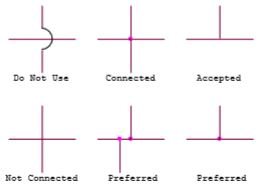
\includegraphics[width=0.5\textwidth]{fig_motor/Schematic/CrossingConnection.jpg}
	\caption[Net verbinden/�berbr�cken]{Net verbinden/�berbr�cken\protect\footnotemark}
	\label{CrossingConnection}
\end{figure}
\footnotetext{\url{http://www.k-state.edu/ksuedl/publications/Technote\%208\%20-\%20Guidelines\%20for\%20Drawing\%20Schematics.pdf}}


\newpage
\subsection{HElicopter Libary}
Auf der Bibliothek von Eagles k�nnen unter der Rubrik \emph{Downloads} Bauteile zu denn Schaltpl�nen gefunden werden. Die dort vorhandenen Bibliotheken sind von Usern bereitgestellt worden. Deshalb besteht die M�glichkeit, dass Bauteile fehlerhaft sind.

Wenn in der Bibliothek kein Element f�r das Bauteil gefunden werden konnte, muss dieses erstellt und in der bereits vorhandene Libary \textit{HElicopterLib.lbr} hinzugef�gt werden. In dieser Libary sind alle Teile festgehalten, die f�r die Quadrocopter ben�tigt werden. 

Ein Bauteil oder auch ein Device besteht aus insgesamt drei eigenen Bestandteilen, die alle vorhanden sein m�ssen, um das Bauteil zu verwenden:
\begin{center}
	\begin{tabular}{l p{10 cm} }
	Symbol & Darunter versteht man eine schematische Skizze eines Bauteils. Alle Schnittstellen des Bauteiles sind zu erkennen und ggf. zu kennzeichen. \newline Der Orignalma�stab und Echtheit der Pinanordnung spielt keine Rolle. Diese soll m�glichst so platziert werden, um im sp�teren Layout eine gewisse �bersichtlichkeit zu wahren. Die Namen der Pins sollen so benannt werden, wie diese vom Hersteller in den Datenbl�ttern festgelegt ist. Ansonsten k�nnte es Sp�ter Probleme zur Pin-Zuordnung geben \newline Die Schl�sselw�rter \textit{>NAME} und \textit{>VALUE} sollen sich (wenn m�glich) im Symbol befinden. \\
	Package & In dieser Skizze soll eine realit�tsnahe Abbildung des Bauteiles erstellt werden, mit original Abmessungen wie z.B. Platinengr��e, Platinenform, Pins und Bohrl�cher, die aus den jeweiligen Datenbl�ttern ersichtlich sind. 
	Weitere Erg�nzungen sind sonstige Bauteile oder SMD auf einem Device sowie deren Verbindungen auf Ober- bzw. Unterseite. Diese werden derzeit nicht ben�tigt und wurden deshalb weggelassen. \\
	Device & In einem Device werden ein Symbol und ein Package miteinander zusammengef�gt. Die Pins aus dem Symbol und Package Skizzen werden  miteinander verkn�pft. Wenn jeder Pin zugeordnet wurde kann das Device verwendet werden.\\
	\end{tabular}
\end{center}

Der Vorteil dieser Aufteilung ist der, dass einzelne Packages und Symbole f�r mehrere Devices verwendet werden k�nnen. Nur die Anzahl der Pins aus den Packages und Symbolen m�ssen eindeutig �bereinstimmen und zugewiesen werden.

\subparagraph{Um bereits existierende Libaries hinzuzuf�gen} wird die gew�nschte Libary in dem Ordner EAGLE-7.5.0/*lbrName* gespeichert. Anschlie�end klickt man im Reiter \emph{Bibliothek} auf \emph{Benutzen} und w�hlt die gew�nschte Libary aus. Ein Schaltplan muss hierbei ge�ffnet sein. Im \textit{Controll Panel} ist das Hinzuf�gen von libaries nicht m�glich. Zuletzt m�ssen die libaries noch aktualisiert werden( unter \emph{Bibliothek} auf die Rubrik \emph{Alle Aktualisieren}). Abschlie�end auf  \textit{ Add/Neues Bauteil hinzuf�gen}, es erscheint die Libary in der Liste. 

\subparagraph{Um ein vorhandenes Bauteil in die eigene Libary einzuf�gen} muss die Ziel-Libary ge�ffnet sein. Im \textit{Control Panel} von EAEGLE( in der linken Spalte das Men� \textit{Bibliotheken} �ffnen). Hier sollten sich alle bereits hinzugef�gten Libaries befinden. Ist dies nicht der Fall: rechtsklick auf die \textit{Bibliotheken} und  \textit{alle Bibliotheken laden} ausw�hlen. Nun muss die Quell-Libary des Bauteils ge�ffnet werden.Das zu kopierende Bauteil rechts klicken und \textit{In Bibliothek} ausw�hlen. Es ist auch m�glich, einzelne Packages oder Symbole neben ganzen Bauteilen/Devices zu kopieren. Nun sollte das hinzugef�gte Objekt in der Ziel-Libary ge�ffnet sein. Best�tigen sie das Hinzuf�gen mit Speichern der Libary.

\subparagraph{F�r das Bearbeiten existierender Libaries} �ffnen sie eine schematische Skizze. Klicken sie auf \textit{Bibliothek}, dann \textit{�ffnen..} und w�hlen sie die zu �berarbeitende Libary aus. Nun k�nnen alle existierende Bauteile, Packages und Symbole bearbeitet oder neue erstellt werden.
Nach der �nderung speichern Sie die Libary und klicken sie auf wieder auf Bibliothek. Anschlie�end aktualisieren Sie die Libaries. Die �nderungen sollten nun vorgenommen sein.

\textit{Achtung:} �nderungen werden auf alle bestehenden und eingef�gten Elementen vorgenommen. Dies kann sich z.B. unvorteilhaft auf die Lesbarkeit auswirken. Aus diesem Grund sollte zumindest eine Kopie des ge�nderten Devices oder eine neue Version erstellt werden. 


%% Project Goals
%--------------------------------------------
% Chapter: PROJECT GOALS
%--------------------------------------------
\chapter{Project's context and goals}
\label{sec:projGoals}

The very first target was to adapt a new hardware (Raspberry Pi) including a autonomous landing to the Quadrocopter from Hochschule Esslingen (HElikopter). As this was not enough work for all of us, the project was extended to include a autonomous landing, too. We were a team of 4 students who were interested in a project work with the HElikopter. We internally agreed in splitting the work in 2 parts. The other two students were more interested in developing the new hardware platform and software and we liked to care about the autonomous landing.

As we developed the autonomous landing to the new hardware, there was a slight dependence to each other.
Following are the goals:
\begin{itemize}
	\item Autonomous Landing
	\item Effective Distance measurement to ground
	\item Implementation on Raspberry Pi
\end{itemize}

This document describes a project in the context of the curriculum's module 'project work' of the masters program Software-based Automotive Systems. The project intends to set up a generic hardware and software platform to control the HElikopter Quadrocopters of Hochschule Esslingen, Faculty Information Technology. The platform shall be based on a real-time capable Linux Operating System and a Raspberry Pi B+ Board. Furthermore, all components used shall be available on market as much ready-made as possible.

Originally, the project was designed to be elaborated by a group of four students. Unfortunately, two students had to face some substantial problems during the project work. Eventually, the project got split up into two separated groups. In consequence, the initially intended goals could not be reached completely. This is partly reflected in the below shown tasks, milestones and project goals.

\begin{figure}[h]
    \centering
    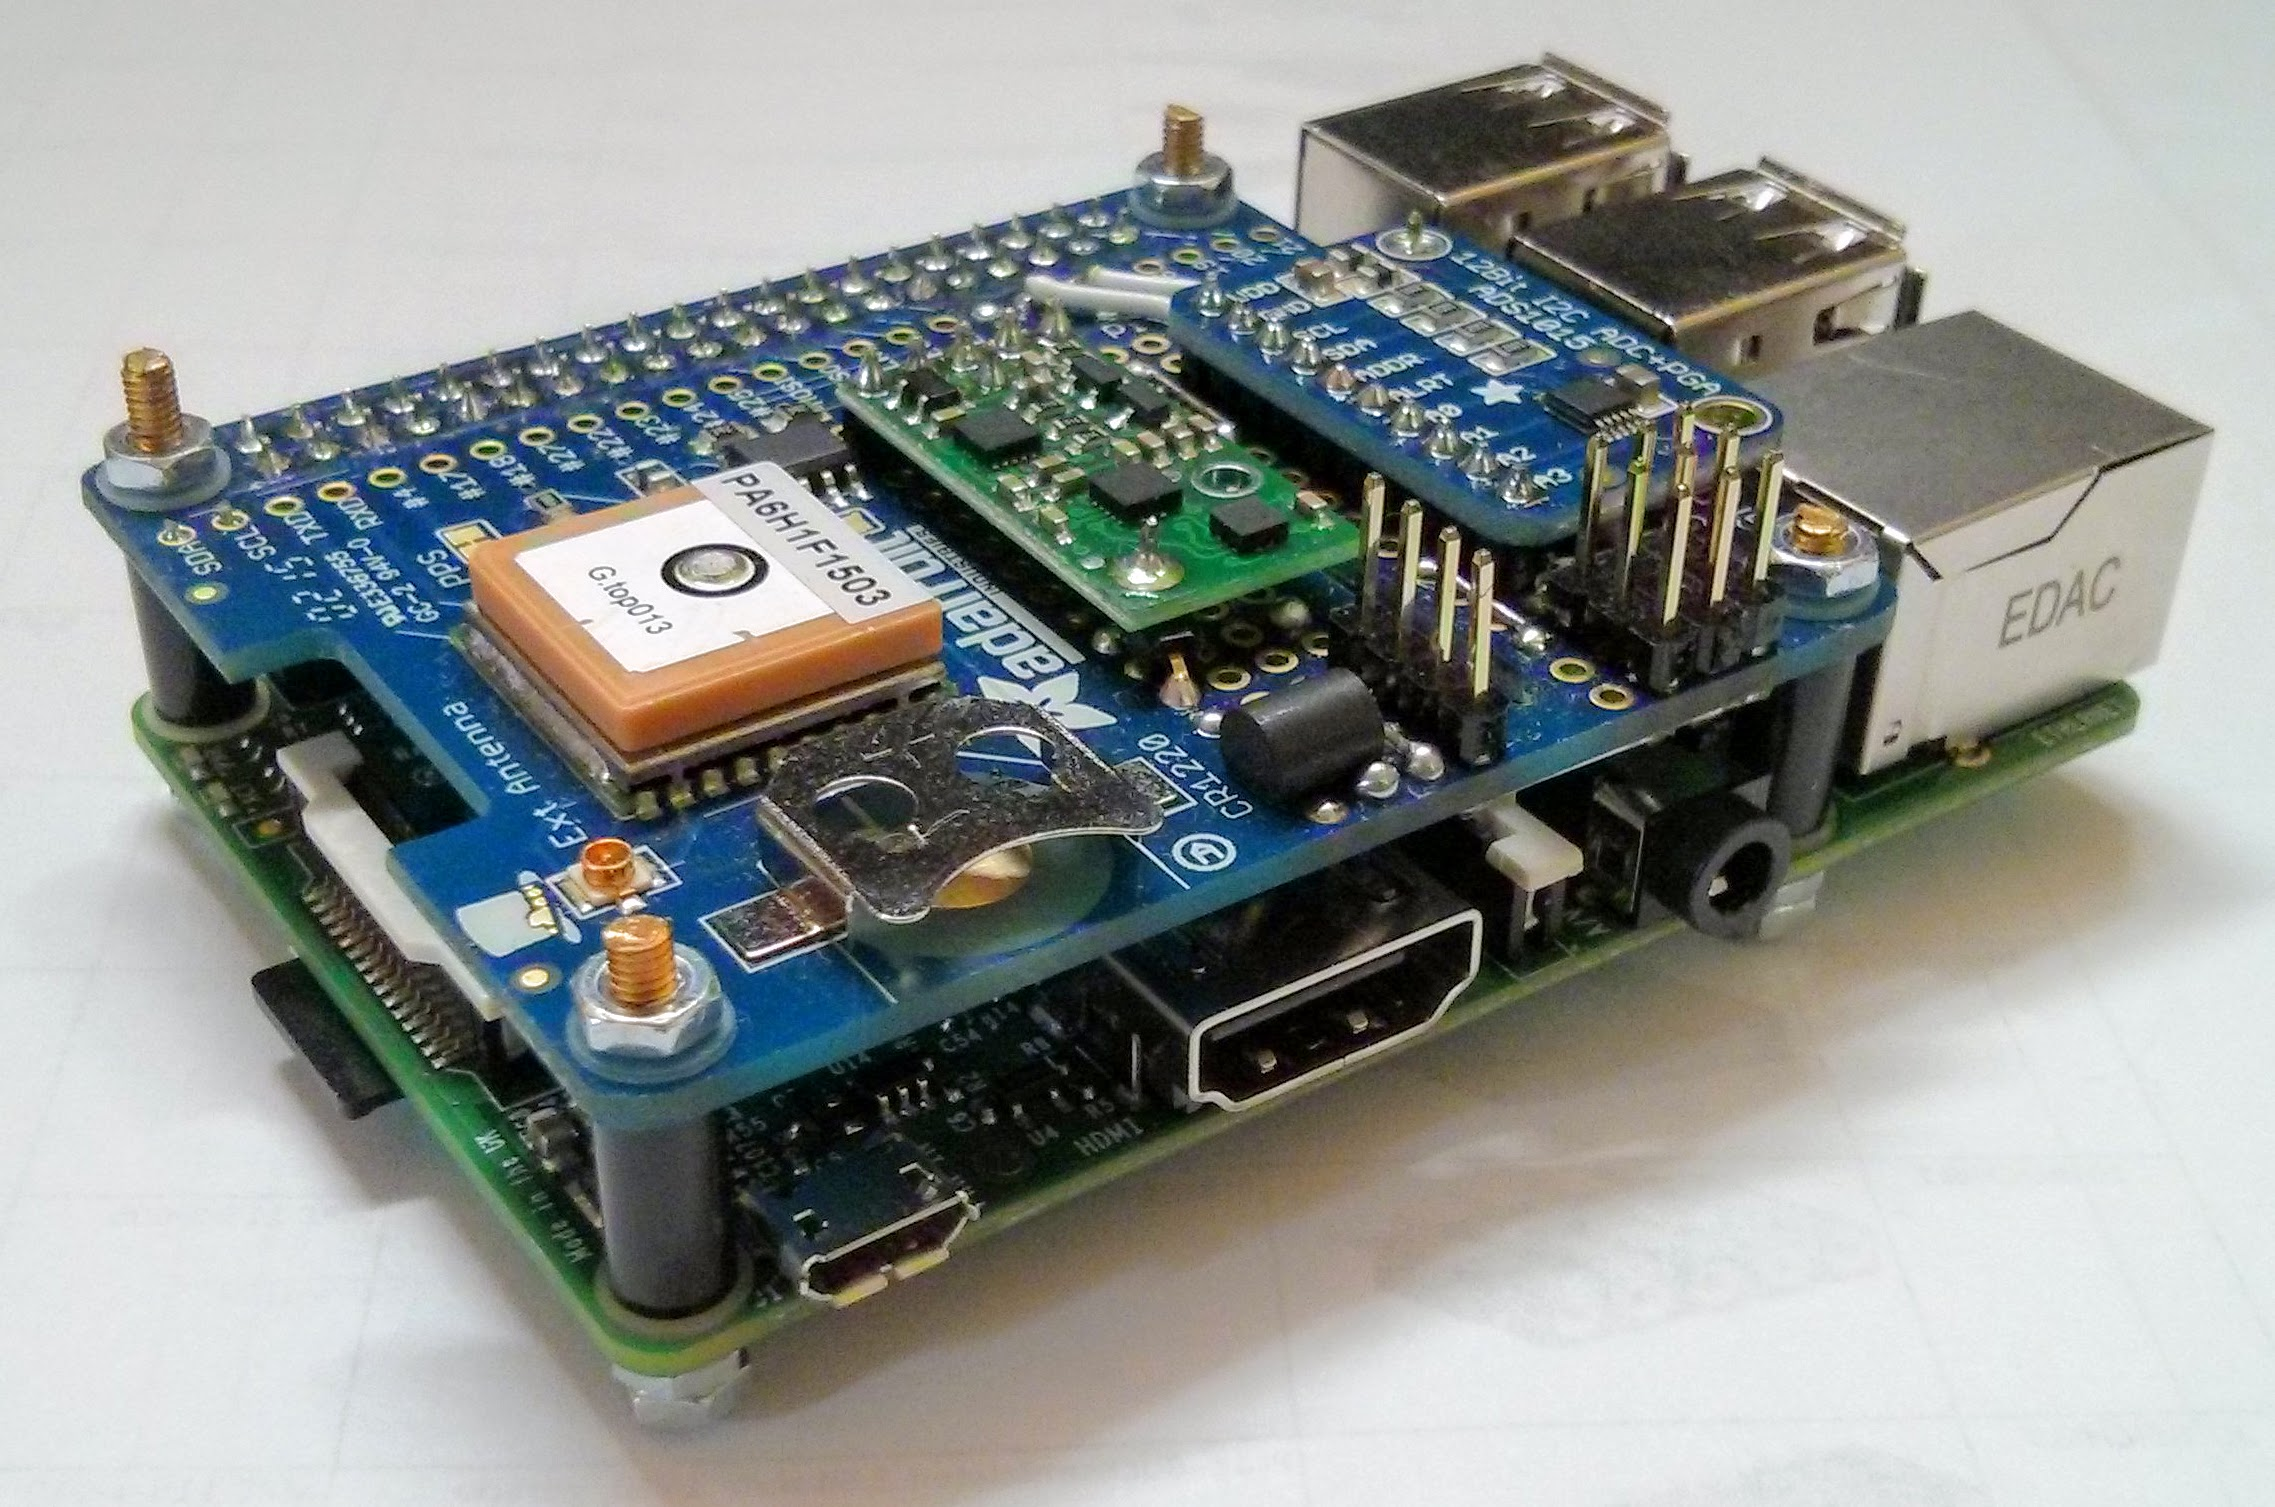
\includegraphics[width=0.85\textwidth]{fig/ch-project-goals/MainRaspberryPi}
    \caption{Raspberry Pi based Quadrocopter Platform (Controller Board)}
    \label{fig:projGoals:RpiPic}
\end{figure}

Nevertheless, the authors of this document are confident that the shown Raspberry Pi based platform is a solid and stable approach. With some extensions on this work, a Linux-driven Quadrocopter can be realized in a future project work.

%- - - - - - - - - - - - - - - - - - - - - - 
% Section: Temporal project scope
%- - - - - - - - - - - - - - - - - - - - - - 
\section{Temporal project scope}
\label{sec:projGoals:temporalProj}
The project started in \textbf{March 23, 2015} and ended in \textbf{June 26, 2015}.

The following milestones were initially set up:
\begin{table}[H]	
	\begin{tabular}{|c|c|c|c|}
\hline
&&&\\
\textbf{Nr.} & \textbf{Date} & \textbf{Milestone's goal} & \textbf{Status}\\
&&&\\
\hhline{|=|=|=|=|}
&&&\\
	1 & April 1, 2015 & Hardware selected & \textcolor[rgb]{0,0.58,0}{\textbf{successfully reached}}\\
	&&&\\
\hline
&&&\\
				2 & May 11, 2015 & HAL drivers finalized& \textcolor[rgb]{0,0.58,0}{\textbf{successfully reached}}\\
				&&&\\
\hline
&&&\\
				3 & May 25, 2015&First prototyp with flying capabilities& \textcolor[rgb]{1,0.41,0.13}{\textbf{partly reached}}\\
				&&&\\
\hline
&&&\\
				4 & June 15, 2015& First prototyp with position hold &\textcolor[rgb]{1,0,0}{\textbf{not reached}}\\
				&&&\\
\hline
	\end{tabular}
	\caption{Initially set up milestones for the project MasterQuad 2015}
	\label{tab:projGoals:milestones}
\end{table}
%\begin{enumerate}
	%\item \textbf{Milestone}: \textcolor[rgb]{0,0.58,0}{(\textbf{successfully reached})}\\
				%\textbf{Date}: April 1, 2015\\
				%\textbf{Goal}: Hardware selected
	%\item \textbf{Milestone}: \textcolor[rgb]{0,0.58,0}{(\textbf{successfully reached})}\\
				%\textbf{Date}: May 11, 2015\\
				%\textbf{Goal}: HAL drivers finalized
	%\item \textbf{Milestone}: \textcolor[rgb]{1,0.41,0.13}{(\textbf{partly reached})}\\
				%\textbf{Date}: May 25, 2015\\ 
				%\textbf{Goal}: First prototyp with flying capabilities
				%
	%\item \textbf{Milestone (optional)}: \textcolor[rgb]{1,0,0}{(\textbf{not reached})}\\
				%\textbf{Date}: June 15, 2015\\
				%\textbf{Goal}: First prototyp with position hold
%\end{enumerate}

%- - - - - - - - - - - - - - - - - - - - - - 
% Section: Contentual project scope
%- - - - - - - - - - - - - - - - - - - - - - 
\section{Contentual project scope}
\label{sec:projGoals:projPlan:cententual}
The original project goals where defined as followed:
\begin{enumerate}
	\item Select new hardware (Raspberry-based with Linux capability) 
	\item Setting up RTOS (Preempt RT Kernel)
	\item Writing HAL drivers for new Hardware
	\item Writing a sensor fusion for orientation filtering and signal enhancement
	\item Integrate existing control software (if possible)
	\item Setup of flight model to simulate position hold
	\item Implement controllers for position hold
\end{enumerate}

Not all goals could be successfully reached - items 5 to 7 could not be completely realized within the project time. Nevertheless, a stable and performant core system has been set up that can be utilized for further projects and applications.

%- - - - - - - - - - - - - - - - - - - - - - - 
% Section: Tasks and responsible team members
%- - - - - - - - - - - - - - - - - - - - - - - 
\section{Tasks and responsible team members}
\label{sec:projGoals:tasksAndMembers}

\textemphs{Oliver Breuning} (E-Mail: olbrgs00@hs-esslingen.de)

Responsibilities:
\begin{itemize}
	\item Virtual Machine as Development Environment (see Chapter \ref{sec:sec-VM})
	\item Low-Level-Driver for UART access
	\item HAL-Driver for battery check
	\item HAL-Driver for GPS
	\item HAL-Driver for Barometer
	\item HAL-Driver for Gyroscope
	\item Generic Library for fast Matrix-Operations
	\item Sensor-Fusion for IMU (see Chapter \ref{sec:sensorFusion})
	\item Tilt-compensation for Intertial Measurement Unit (IMU) (see Chapter \ref{sec:angle})
	\item Complementary-Filter (see Chapter \ref{sec:ComplementaryFilter})
	\item Kalman-Filter (see Chapter \ref{sec:KalmanFilter})
\end{itemize}

\vspace{0.5cm}

\textemphs{J\"urgen Schmidt} (E-Mail: juscgs00@hs-esslingen.de)

Responsibilities:
\begin{itemize}
	\item Project management
	\item Hardware layout and mechanical packaging
	\item Software architecture and layout
	\item HAL-Driver for Accelerometer
	\item HAL-Driver for Magnetometer
	\item Live network connection for MATLAB (UDP-based)
	\item Linux Kernel update with PREEMPT\_RT patch
	\item Kernel module for precise PPM measurement
	\item Kernel module for precise time trigger control (unstable yet!)
\end{itemize}


\begin{figure}[H]
    \centering
    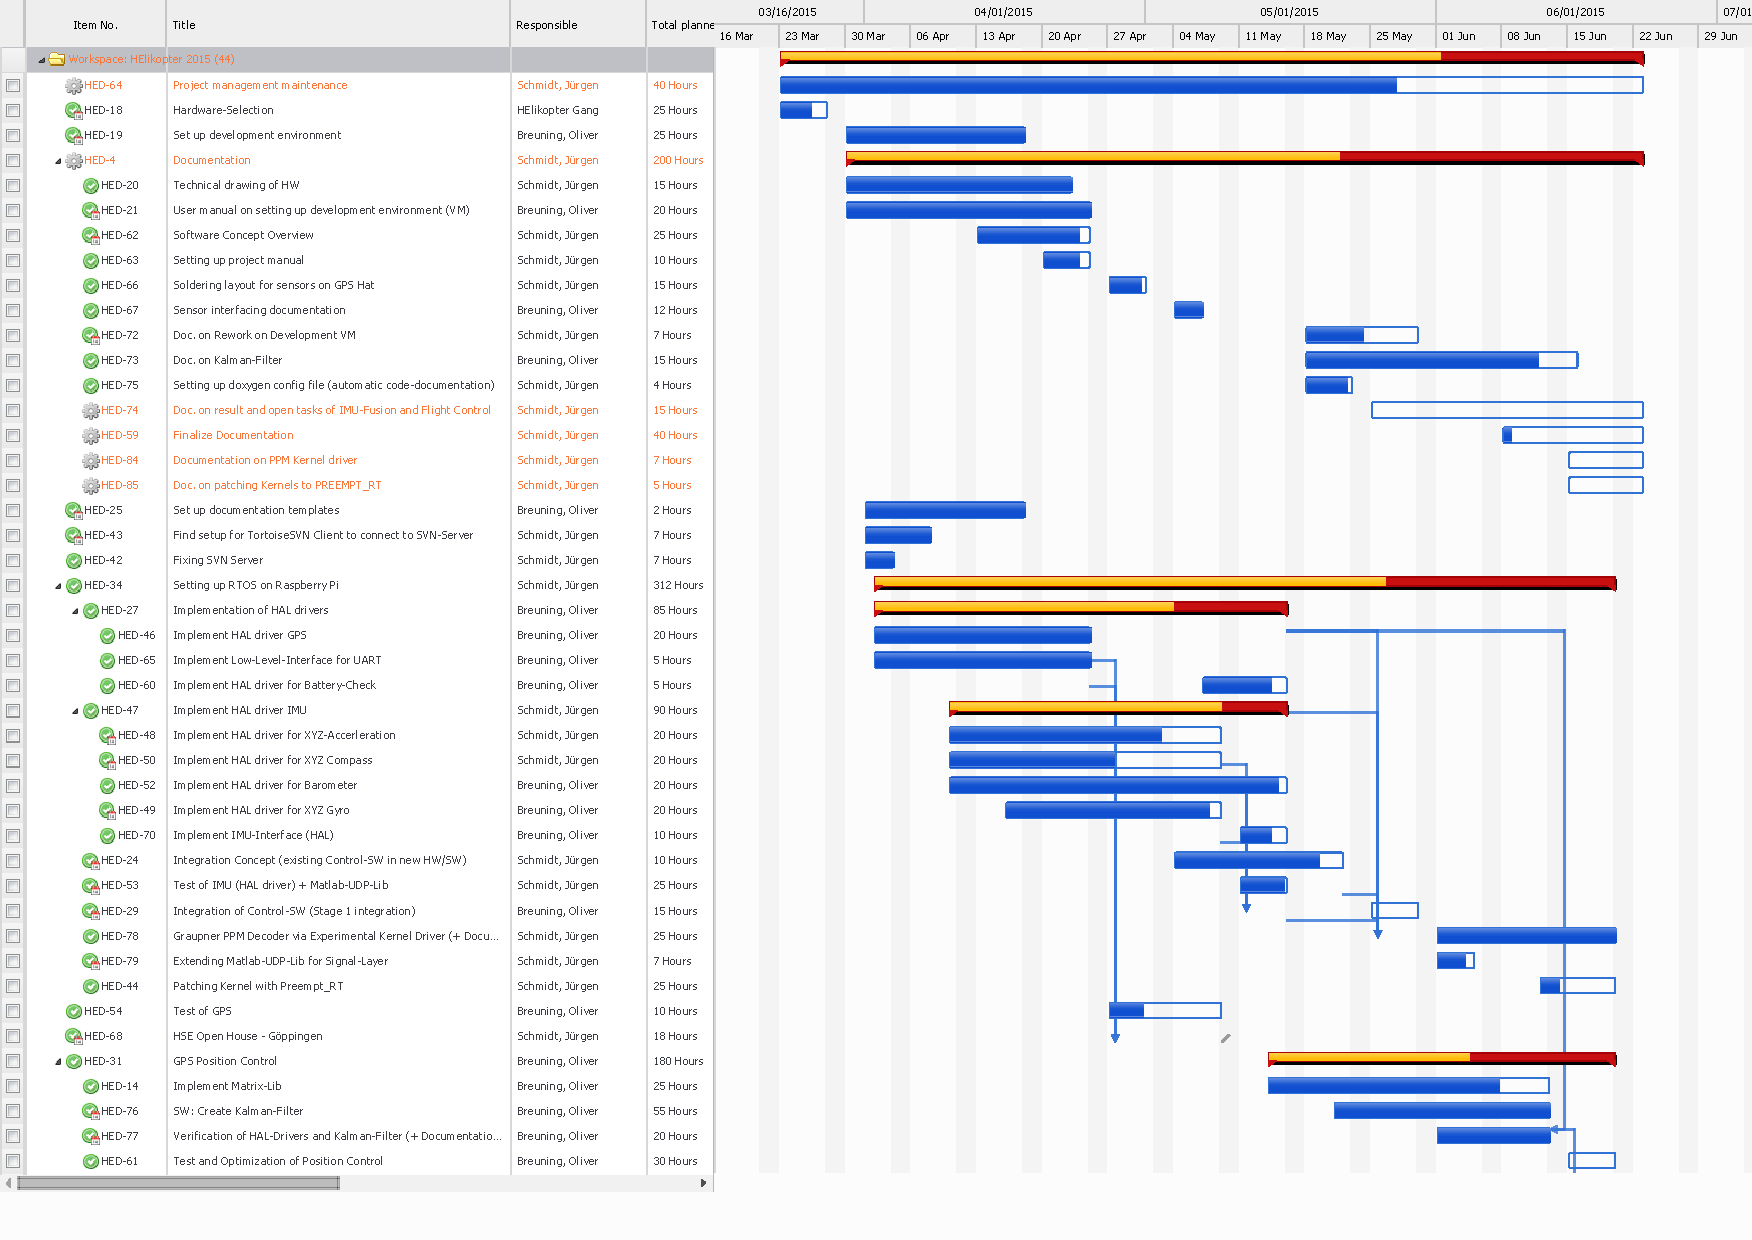
\includegraphics[angle=90,width=\textwidth]{fig/ch-project-goals/project_plan}
    \caption[Gantt diagram of project MasterQuad 2015 (Track+)]{Gantt diagram of the project plan of MasterQuad 2015 (Track+ output)}
    \label{fig:projGoals:ganttDiagram}
\end{figure}

%- - - - - - - - - - - - - - - - - - - - - - - 
% Section: Repository structure
%- - - - - - - - - - - - - - - - - - - - - - - 
\section{Repository structure}
\label{sec:projGoals:repos}

For version controlling, the subversion system of the HElikopter Project has been used. Every team member has regarded the following given folder structure in order to keep a structured and organized working flow.
\dirtree{%
.1 /.
.2 doc\DTcomment{\textbf{Finalized documentation}}.
.3 pm\DTcomment{Documentation regarding project management}.
.4 meetings\DTcomment{Meeting reports and meeting template}.
.4 sources\DTcomment{LaTex sources of all documents in \texttt{/doc/pm}}.
.3 se\DTcomment{Documentation regarding system engineering}.
.4 sources\DTcomment{LaTex sources of all documents in \texttt{/doc/se}}.
.2 impl\DTcomment{\textbf{Source code}}.
.3 branch\DTcomment{Container for parallel development lines to trunk}.
.3 tag\DTcomment{Finalized and stable software}.
.3 trunk\DTcomment{Current development line}.
.4 app\DTcomment{Application Layer Software}.
.4 doc\DTcomment{Automatic code documentation via Doxygen}.
.4 hal\DTcomment{Hardware Abstraction Layer Software}.
.4 kern\DTcomment{Custom Linux Kernel modules}.
.4 matlab\DTcomment{Network connection to MATLAB}.
.4 sig\DTcomment{Signal Processing Layer Software}.
.2 scratch\DTcomment{\textbf{Documents or files in progress, excluding source code}}.
.3 doc\_template\DTcomment{Templates for documentation files (mainly LaTex)}.
.2 sys\DTcomment{\textbf{Firmwares, OS and development environment}}.
.3 RPi\DTcomment{Preconfigured firmware(s) for Raspberry Pi B+}.
.3 VM\DTcomment{Development Environment VM with all IDEs preconfigured}.
}

Within the folders 
\begin{itemize}
	\item \texttt{/impl/trunk/app}
	\item \texttt{/impl/trunk/hal}
	\item \texttt{/impl/trunk/sig}
\end{itemize}
a subfolder for each functional unit shall be created. The functional units shall be considered as depicted in figure \ref{fig:layer:layer_graph} (smaller boxes inside of the colored layers). Example:
\dirtree{%
.1 /.
.2 impl.
.3 trunk.
.4 hal.
.5 adc.
.5 gps.
.5 gyro.
}

\subsection*{Storing test files}
\label{sec:work:groupware:test}
For each software component, a separate test should be written to ensure the software quality. All source code files and test data files to run a test shall be saved in a separate subfolder named \texttt{tst}. Example:
\dirtree{%
.1 /.
.2 impl.
.3 trunk.
.4 hal.
.5 gps.
.6 tst\DTcomment{contains data \& code to test the module 'gps'}.
.7 test\_data.dump.
.7 helper\_code.c.
.7 helper\_code.h.
.7 test\_main.c.
.6 gps.c\DTcomment{actual source of module 'gps'}.
.6 gps.h\DTcomment{actual interfaces of module 'gps'}.
}


\textbf{Important note:}\\
The \texttt{tst}-folder will \textbf{not} be moved to the tags folders! All data in \texttt{/imp/tags} is considered to be well tested and stable. Therefore, the test data is not required to move.

%--------------------------------------------
% section: DOCUMENTATION
%--------------------------------------------
\section{Documentation}
\label{sec:work:docu}
The project team delivered the following documents:
\begin{itemize}
	\item Project manual (\texttt{/doc/pm})
	\item Technical drawings of hardware (\texttt{/doc/se}, see also chapter \ref{sec:hardware:techDrawAndPack})
	\item Bill of materials (\texttt{/doc/se}, see also chapter \ref{sec:hardware:BillOfMat})
	\item Software structure \& concept (\texttt{/doc/se}, see also chapter \ref{sec:software})
	\item User manual of project (this document)
	\item Doxygen-based code documentation (see appendix \ref{sec:b-codeDoc})
\end{itemize}

The doxygen-based code documentation is delivered in the SVN repository as HTML output of the current working copy. The doxygen configuration file has been submitted in \texttt{/impl/trunk/doc/} (see also Appendix \ref{sec:b-codeDoc}). To regenerate the code documentation to the latest version, run \texttt{doxygen} in the above mentioned folder.
%% Landing concept
% Bsp. eines Hauptteils

\chapter{Landing Concept}
\label{cha:LandingCon}


This Chapter is about the (theoretical) ways, how to manage a autonomous landing.

In anyway we need to adjust the speed of the rotors, depending on our measurements.


\section{Challenges}
\label{sec:landcha}

There will be several critical "challenges" during a landing process. Some of them when can estimate before and give a option, how to handle them.


\subsection{Drift}

It is very hard, to keep a Quadrocopter (in our case HElikopter) on a fixed point in a room. There is always a little bit of wind, at least from the Quadrocopter itself. Therefore you always need to correct you position, to avoid it drifting away to one side.\\
With our sensors implemented we can recognize the movement and take some countermeasures.\\

The GPS system won't work indoor, so we need to rely on the IMU (Inertial Measurement Unit). So there is no absolute measurement of the position and we need to do some calculation with the acceleration in XY-Axis, to handle the drift.\\

With the gyroscope we can also handle the drift about our own axis.


\subsection{Orientation}

Because of our limited sensors, and a non working GPS indoor, it will not be possible to get a absolute orientation in a room.\\

Outdoors we can take the GPS with the barometer, the gyroscope and the laser sensor to get a very good knowing of where we are.


\subsection{Distance}

In a steady flight situation, we measure the distance straight to the ground. But when the quadrocopter is moving, we need to calculate the distance to ground with the angle of it.


\subsection{Landing Zone}

The first step will be, to take control of the landing watching with our eyes. Just decreasing the speed of the motors (rotors) depending on the distance to ground.\\

When we try that the Quadrocopter takes care of a free landing zone by itself, we can think about different options:\\

\underline{Circling}

With this method we just fly over the whole landing zone, which is a big as the quadrocopter. When we got the same distance value for the whole area, we can assume that there is no obstacle within it.


\underline{Remembering}

If we take some measurements during normal flight mode, we can save that values and try to build a map of the area under us. With this method we can fly to a "free" landing zone, when the landing mode is enabled.

\underline{lateral buckling}

May be the fastest and the most difficult way to land. By lateral buckling/tilting and calculation of the gathered values (depending on the angle), we can get a fast look over the area under us.

The challenge will be to stay, more or less, on the same position. Considering a certain height, where doing this action, there may be needed only small angles to tilt.

Or we could think about, mounting the laser sensor with a small angle. So to speak with a offset. We can easily consider the angle in the calculation of the height and only need to turn on the quadrocopters z-axis to check the landing zone.

\newpage
\section{Landing Mode}

The Landing mode should handle the landing of the quadrocopter fully autonomous.

\subsection{Activation}

The Landing Mode will/must be activated external. With it some sensor could be activated too, or configured in a other way. 


\subsection{Abort Landing}

We should be able to abort the autonomous landing, if we detect a problem.

1. approach: Just turning the Landing Mode off.

2. approach: Override the Landing Mode with the remote control.

3. approach: Abort the landing and turn the rotors off, to prevent damage to them.






%Verweise im Text: \cite{doc:stz} und \cite{doc:gun}.

\chapter{Open Points}
\label{sec:ergeb}

There are several points we wanted to do, but could not manage to do or finish them in time.

\section{Connecting actuators}

We did not connect any actuator, like an rotor, to our current software. There was no actuator-software ported to our Raspberry Pi to test with our developments.



\section{Reacting on sensor values}

There was no development to react, in any way, on our provided sensor values.\\
For this reason there is no controller yet, processing external signals or work between sensor and actuator.


%\enquote{Neuigkeiten} Messergebnisse




%% Raspberry Pi based hardware platform (hardware)
%--------------------------------------------
% Chapter: RASPBERRY PI BASED HARDWARE PLATFORM
%--------------------------------------------
\chapter{Raspberry Pi based hardware platform}
\label{sec:hardware}
%- - - - - - - - - - - - - - - - - - - - - - 
% Section: Basic components and sensors
%- - - - - - - - - - - - - - - - - - - - - - 
\section{Hardware and device communication}
\label{sec:hardware:Hardware}

%- - - - - - - - - - - - - - - - - - - - - - 
% Subsection: Basic components and sensors
%- - - - - - - - - - - - - - - - - - - - - - 
\subsection{Basic components and chosen sensors}
\label{sec:hardware:Components}

As the main computing board the Raspberry Pi B+ has been chosen. At time of start of this project, there has been no stable Real-Time Kernel Patch (PREEMPT\_RT) for the multi-core CPU Broadcom BCM2709 of Raspberry Pi 2. Fortunately, the 40-pin expansion breakout of Raspberry Pi A+/B+ and Raspberry Pi 2 are identical. In consequence, all the chosen peripheral hardware and sensors are compatible with Raspberry Pi 2. In future projects, it should be a minor task to update the Kernel of the pre-configured OS Image delivered in this project and make a Raspberry Pi 2 running with this platform. A complete list of all components with pictures can be found in chapter \ref{sec:hardware:BillOfMat}.

The main components chosen for this project are:
\begin{itemize}
	\item \textbf{Main board:}\\
	\texttt{Raspberry Pi A+/B+} in this project. In future projects, also the \texttt{Raspberry Pi 2} is compatible with the chosen hardware as soon as a Raspberry Pi 2 compatible PREEMPT\_RT Kernel Patch is available.
	
	\item \textbf{Expansion Board:}\\
	\texttt{Adafruit GPS Hat}, including a \texttt{GlobalTop GPS} receiver with builtin Chip-Antenna. The GPS is connected via UART to the Raspberry Pi board. In consquence, the UART may not be used for other purposes and is blocked when the GPS Hat is assembled to the Raspberry Pi!
	
	\item \textbf{Inertial Measurement Unit (IMU):}\\
	\texttt{Polulu AltiIMU v4 (10-DOF version)}. The Inertial Measurement Unit comprises sensors that enables to measure the pose of the Quadrocopter in space. Rotational speed, acceleration rates for each axis in space and the barometric air pressure can be sensed with the chosen IMU. The IMU is connected via I2C to the Raspberry Pi board.
	
	In consequence, the following sensors are included in the chosen IMU:
	\begin{itemize}
		\item \textbf{3D Accelerometer:} \texttt{ST LSM303D} (including 3D Magnetometer/e-Compass)
		\item \textbf{3D MEMS Gyroscope:} \texttt{ST L3GD20H}
		\item \textbf{3D Magnetometer:} \texttt{ST LSM303D} (including 3D Accelerometer)
		\item \textbf{Absolute MEMS Barometer:} \texttt{ST LPS331AP}
	\end{itemize}
	
	\item \textbf{A/D Converter:}\\
	\texttt{Adafruit ADS1015} including ADC Chip \texttt{Texas Instruments ADS1015}. The ADC breakout board is connected via I2C to the Raspberry Pi board.
	
	\item \textbf{DC/DC Power converter:}\\
	\texttt{Polulu D15V70F5S3}. Since the Raspberry Pi board including all peripherals is aimed to be connected to the Li-Ion battery of the HElikopter Quadrocopters of Hochschule Esslingen, a separate DC/DC power converter has been included to the controller platform. The power converter ensures a stable power supply voltage of 5V DC at a continuous current draw up to 3.5A.
\end{itemize}

%- - - - - - - - - - - - - - - - - - - - - - 
% Subsection: I2C Adressing
%- - - - - - - - - - - - - - - - - - - - - - 
\subsection{I2C adressing}
\label{sec:hardware:Components:Adressing}

This section shows all necessary transmissions which are needed for a successful interfacing on the I$^2$C bus. 

\begin{itemize}
	\item \subsubsection{\underline{\textbf{A/D Converter}}}
\label{sec:hardware:Components:Adressing:ADC}

%\textbf{I$^2$C slave adress:\\
\textbf{I$^2$C slave address}: \texttt{0b1001001 (0x49)}

\subsubsection{Read}
\label{subsec:ADCread}

The read command get's the data from the address, which is stored in the pointer register (blue color). See figure \ref{fig:ADC1}

\begin{figure}[H]
	\centering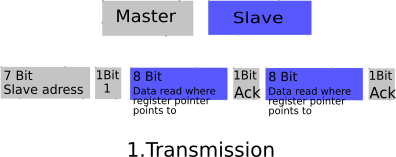
\includegraphics[width=0.7\textwidth]{fig/I2C_Adressing/ADC_read}
	\caption{Scheme to read data from the ADC}
	\label{fig:ADC1}
\end{figure}

\subsubsection{Write}
\label{subsec:ADCwrite}


\begin{figure}[H]
	\centering\includegraphics[width=0.7\textwidth]{fig/I2C_Adressing/ADC_write}
	\caption{Scheme to write data to the ADC}
	\label{fig:ADC2}
\end{figure}

\subsubsection{Read conversion register}
\label{subsec:ADCconversion}
To enable a read from a conversion register, several packages need to be sent. They can be seen in figure \ref{fig:ADC3}. All slave and master acknowledges are not shown because they are handled direct by the interface and so not important for the application.

\begin{figure}[H]
	\centering\includegraphics[width=0.9\textwidth]{fig/I2C_Adressing/ADC_read_conversion}
	\caption[Scheme to read the ADC's conversion registers]{Transmission scheme to read the ADC's conversion registers}
	\label{fig:ADC3}
\end{figure}

\item \subsubsection{\underline{\textbf{Inertial Measurement Unit (IMU)}}}
\label{sec:hardware:Components:Adressing:IMU}

The Inertial measurement unit (IMU) has three different chips mounted. Each chip solves one of the measurements of this unit. Each chip has a different I$^2$C address. All slave and master acknowledges are not shown because they are handled direct by the interface and are not important to the application level.
 \begin{itemize}
	 \item \subsubsection*{\underline{\textbf{Acceleration and Magnet Sensor}}}
\label{sec:hardware:Components:Adressing:IMU:ACC}

\textbf{I$^2$C slave address}: \texttt{0b0011110 (0x1E)}

There are several registers which have to be configured before reading and also several register where the acceleration, magnetic strength and if needed temperature can be read. To reduce the amount of pages of this document, they will be not listed here. All the registers can be found in the datasheet \texttt{IMU\_LSM303D.pdf}, stored in the SVN directory \texttt{/doc/se/Datasheets/IMU}.


\subsubsection{Read}
\label{subsubsec:ACCread}

\begin{figure}[H]
	\centering\includegraphics[width=0.7\textwidth]{fig/I2C_Adressing/ACC_read_single}
	\caption{Transmission scheme for a single byte read of the ACC-Sensor}
	\label{fig:ACC1}
\end{figure}

\begin{figure}[H]
	\centering\includegraphics[width=0.8\textwidth]{fig/I2C_Adressing/ACC_read_multiple}
	\caption[Scheme for multiple data read of the ACC-Sensor]{Transmission scheme for multiple data read of the ACC-Sensor(burst read)}
	\label{fig:ACC2}
\end{figure}

\textbf{1. Transmission}: Slave address including RW bit ('0'): \texttt{0x3C}\\
\textbf{2. Transmission}: Slave address including RW bit ('1'): \texttt{0x3D}

\subsubsection{Write}
\label{subsubsec:ACCwrite}

\begin{figure}[H]
	\centering\includegraphics[width=0.55\textwidth]{fig/I2C_Adressing/ACC_write_single}
	\caption[Scheme for a single byte write of the ACC-Sensor]{Transmission scheme for a single byte write of the ACC-Sensor}
	\label{fig:ACC3}
\end{figure}

\begin{figure}[H]
	\centering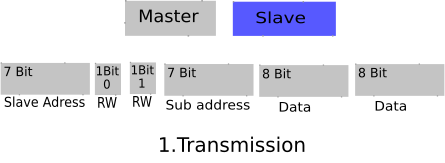
\includegraphics[width=0.7\textwidth]{fig/I2C_Adressing/ACC_write_multiple}
	\caption[Scheme for multiple data write of the ACC-Sensor]{Transmission scheme for multiple data write of the ACC-Sensor(burst write)}
	\label{fig:ACC4}
\end{figure}

\textbf{1.Transmission}: Slave address including RW bit ('0'): \texttt{0x3C}


\item \subsubsection*{\underline{\textbf{Gyroscope Sensor}}}
\label{sec:hardware:Components:Adressing:IMU:Gyro}

\textbf{I$^2$C slave address}: \texttt{0b1101010 (0x6A)}

There are several registers which have to be configured before reading and also several register where the rotational speed and if needed the temperature can be read. To reduce the amount of pages of this document, they will be not listed here. All the registers can be found in the datasheet \texttt{IMU\_L3GD20H.pdf}, which is stored in the SVN directory \texttt{\textbackslash{}doc\textbackslash{}se\textbackslash{}Datasheets\textbackslash{}IMU}.

\subsubsection{Read}
\label{subsubsec:Gyroread}

\begin{figure}[H]
	\centering\includegraphics[width=0.7\textwidth]{fig/I2C_Adressing/ACC_read_single}
	\caption{Transmission scheme for a single byte read of the Gyro-Sensor}
	\label{fig:Gyro1}
\end{figure}

\begin{figure}[H]
	\centering\includegraphics[width=0.8\textwidth]{fig/I2C_Adressing/ACC_read_multiple}
	\caption[Scheme for multiple data read of the Gyro-Sensor]{Transmission scheme for multiple data read of the Gyro-Sensor (burst read)}
	\label{fig:Gyro2}
\end{figure}

\textbf{1.Transmission}: Slave address including RW bit ('0'): \texttt{0xD4}\\
\textbf{2.Transmission}: Slave address including RW bit ('1'): \texttt{0xD5}

\subsubsection{Write}
\label{subsubsec:Gyrowrite}

\begin{figure}[H]
	\centering\includegraphics[width=0.55\textwidth]{fig/I2C_Adressing/ACC_write_single}
	\caption[Scheme for a single byte write of the Gyro-Sensor]{Transmission scheme for a single byte write of the Gyro-Sensor}
	\label{fig:Gyro3}
\end{figure}

\begin{figure}[H]
	\centering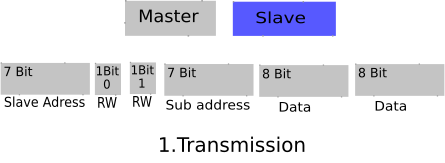
\includegraphics[width=0.7\textwidth]{fig/I2C_Adressing/ACC_write_multiple}
	\caption[Scheme for multiple data write of the Gyro-Sensor]{Transmission scheme for multiple data write of the Gyro-Sensor (burst write)}
	\label{fig:Gyro4}
\end{figure}

\textbf{1.Transmission}: Slave address including RW bit ('0'): \texttt{0xD4}

\item \subsubsection*{\underline{\textbf{Pressure Sensor}}}
\label{sec:hardware:Components:Adressing:IMU:Pressure}

\textbf{I$^2$C slave address}: \texttt{0b1011100 (0x5C)}

There are several registers which have to be configured before reading and also several register where the pressure and if needed the temperature can be read. To reduce the amount of pages of this document, they will be not listed here. All the registers can be found in the datasheet \texttt{IMU\_LPS331AP.pdf}, which is stored in the SVN directory \texttt{\textbackslash{}doc\textbackslash{}se\textbackslash{}Datasheets\textbackslash{}IMU}.

\subsubsection{Read}
\label{subsubsec:Pressureread}

\begin{figure}[H]
	\centering\includegraphics[width=0.7\textwidth]{fig/I2C_Adressing/ACC_read_single}
	\caption[Scheme for a single byte read of the Pressure-Sensor]{Transmission scheme for a single byte read of the Pressure-Sensor}
	\label{fig:Pressure1}
\end{figure}

\begin{figure}[H]
	\centering\includegraphics[width=0.80\textwidth]{fig/I2C_Adressing/ACC_read_multiple}
	\caption[Scheme for multiple data read of the Pressure-Sensor]{Transmission scheme for multiple data read of the Pressure-Sensor(burst read)}
	\label{fig:Pressure2}
\end{figure}

\textbf{1.Transmission}: Slave address including RW bit ('0'): \texttt{0xB8}\\
\textbf{2.Transmission}: Slave address including RW bit ('1'): \texttt{0xB9}

\subsubsection{Write}
\label{subsubsec:Pressurewrite}

\begin{figure}[H]
	\centering\includegraphics[width=0.55\textwidth]{fig/I2C_Adressing/ACC_write_single}
	\caption[Scheme for a single byte write of the Pressure-Sensor]{Transmission scheme for a single byte write of the Pressure-Sensor}
	\label{fig:Pressure3}
\end{figure}

\begin{figure}[H]
	\centering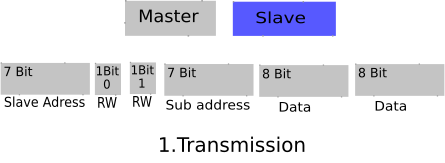
\includegraphics[width=0.7\textwidth]{fig/I2C_Adressing/ACC_write_multiple}
	\caption[Scheme for multiple data write of the Pressure-Sensor]{Transmission scheme for multiple data write of the Pressure-Sensor(burst write)}
	\label{fig:Pressure4}
\end{figure}

\textbf{1.Transmission: Slave address including RW bit ('0'): 0xB8}
\end{itemize}

\item \subsubsection{\underline{\textbf{Motor Driver}}}
\label{sec:hardware:Components:Adressing:IMU:ADC}

All slave and master acknowledges are not shown because they are handled direct by the interface and so not important here. To enable flying with a Quadrocopter there are four motors and so four brushless drivers needed. Each of them has an individual address.

\pagebreak[3]{
\textbf{I$^2$C slave addresses}:\\
Motor 1  --> \texttt{0b0101001 (0x29)}\\
Motor 2  --> \texttt{0b0101010 (0x2A)}\\
Motor 3  --> \texttt{0b0101011 (0x2B)}\\
Motor 4  --> \texttt{0b0101100 (0x2C)}}

\subsection{Read}
\label{subsec:Motorread}

\textbf{Read operations}: NOT DEFINED	

\subsection{Write}
\label{subsec:Motorwrite}

\textbf{Write operations}:

Possible data values are in the range of \texttt{10} (Decimal) up to \texttt{255} (Decimal) which refers to a hexadecimal range of \texttt{0x0A} to \texttt{0xFF}.

\begin{figure}[H]
	\centering\includegraphics[width=0.4\textwidth]{fig/I2C_Adressing/Motor_write}
	\caption[Scheme for a single byte write to a motor driver board]{Transmission scheme for a single byte write to a motor driver board}
	\label{fig:Motor}
\end{figure}


\pagebreak[3]{
\textbf{1.Transmission}: Slave address including RW bit ('0'):\\
Motor 1 --> \texttt{0x52}\\
Motor 2 --> \texttt{0x54}\\
Motor 3 --> \texttt{0x56}\\
Motor 4 --> \texttt{0x58}}

\textbf{Possible Data values are in the range of 10 (Decimal) up to 255 (Decimal). So in the range from 0x0A to 0xFF.}

\end{itemize}

%- - - - - - - - - - - - - - - - - - - - - - 
% Section: UART communication
%- - - - - - - - - - - - - - - - - - - - - - 
\subsection{UART communication}
\label{sec:hardware:Components:UART}
The GPS module uses the UART interface of the Raspberry Pi. The used GPS module has a fixed communication set up.\\
To ensure working the following values need to be used:
\begin{itemize}
	\item Baudrate: 9600 baud
	\item Databits: 8 Bits
	\item Stopbits:	1 Bit
	\item Modem control: No
\end{itemize}


%- - - - - - - - - - - - - - - - - - - - - - 
% Section: Technical drawings and packaging
%- - - - - - - - - - - - - - - - - - - - - - 
\section{Technical drawings and packaging}
\label{sec:hardware:techDrawAndPack}

\begin{figure}[H]
    \centering
    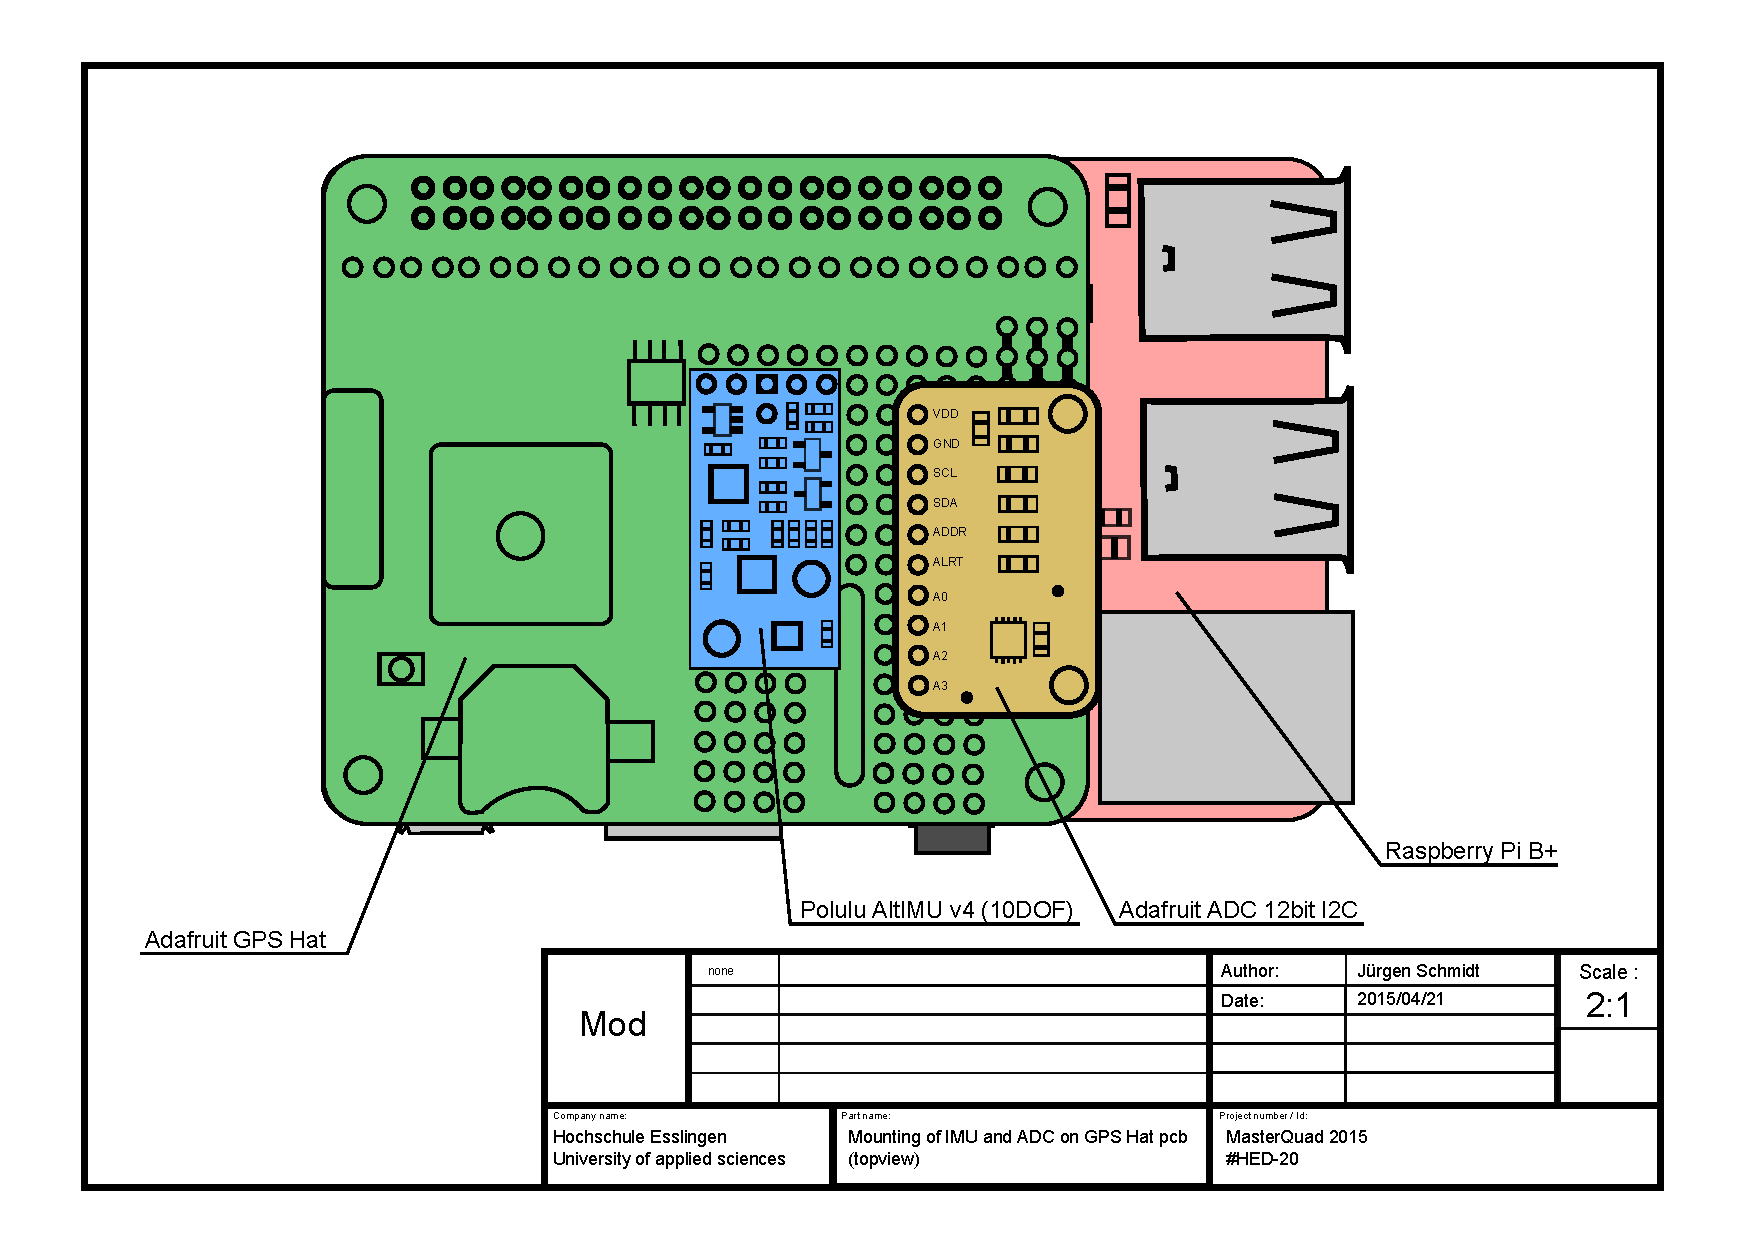
\includegraphics[angle=90,width=0.83\textwidth]{fig/ch-rpi-hardware/A4_tech_draw_topview_sensor_mountingPositions}
    \caption[Placing ADC and IMU on GPS Hat]{Placing ADC and IMU on GPS Hat. The drawing shows the exact position of the sensor boards, aligned with matching soldering pads of the GPS Hat and the Sensor baords.}
    \label{fig:hardware:sensorMount}
\end{figure}

To mount the assembled GPS Hat on top of the Raspberry Pi (as depicted in fig. \ref{fig:hardware:stackedMount}) the following parts are required:
\begin{itemize}
	\item 4 pcs. polyamid standoffs, 10mm height (B\"urklin, 18H5045)
	\item 4 pcs. threaded rod, M2.5 in 40mm pieces (B\"urklin, 16H322)
	\item 16 pcs. polyamid shims, M2.5 (B\"urklin, 16H942)
	\item 12 pcs. hexagonal nuts, M2.5 (B\"urklin, 16H722)
	\item 1 pc. GPS Hat with assembled sensors/peripherals as shown in fig. \ref{fig:hardware:sensorMount} and soldered according to \ref{fig:hardware:soldering:top} and fig. \ref{fig:hardware:soldering:bottom}
	\item 1 pc. Raspberry Pi A+/B+/2
\end{itemize}
All referenced parts are also mentioned in the Bill of Materials in Chapter \ref{sec:hardware:BillOfMat}.

\begin{figure}[H]
    \centering
    \includegraphics[width=0.87\textwidth]{fig/ch-rpi-hardware/A4_tech_draw_sideview_stackedMount}
    \caption{Stacked mounting of Hat-Board on Raspberry Pi}
    \label{fig:hardware:stackedMount}
\end{figure}

To ease the soldering of the IMU and ADC on top of the GPS Hat board, a soldering layout has been created as shown in fig. \ref{fig:hardware:soldering:top} and fig. \ref{fig:hardware:soldering:bottom}. The layout shows in a one-by-one view the soldering pads of the GPS Hat (one view onto the top, one view onto the bottom). According to the experience of the authors of this document, the soldering layout figures eases the soldering of the sensors to the GPS Hat for students, that are not used to solder a densely packed PCB.

\begin{figure}[H]
    \centering
    \includegraphics[width=0.87\textwidth]{fig/ch-rpi-hardware/A4_tech_draw_topview_gpshat_soldering}
    \caption{Soldering plan for Raspberry Pi Hat (top view)}
    \label{fig:hardware:soldering:top}
\end{figure}

\begin{figure}[H]
    \centering
    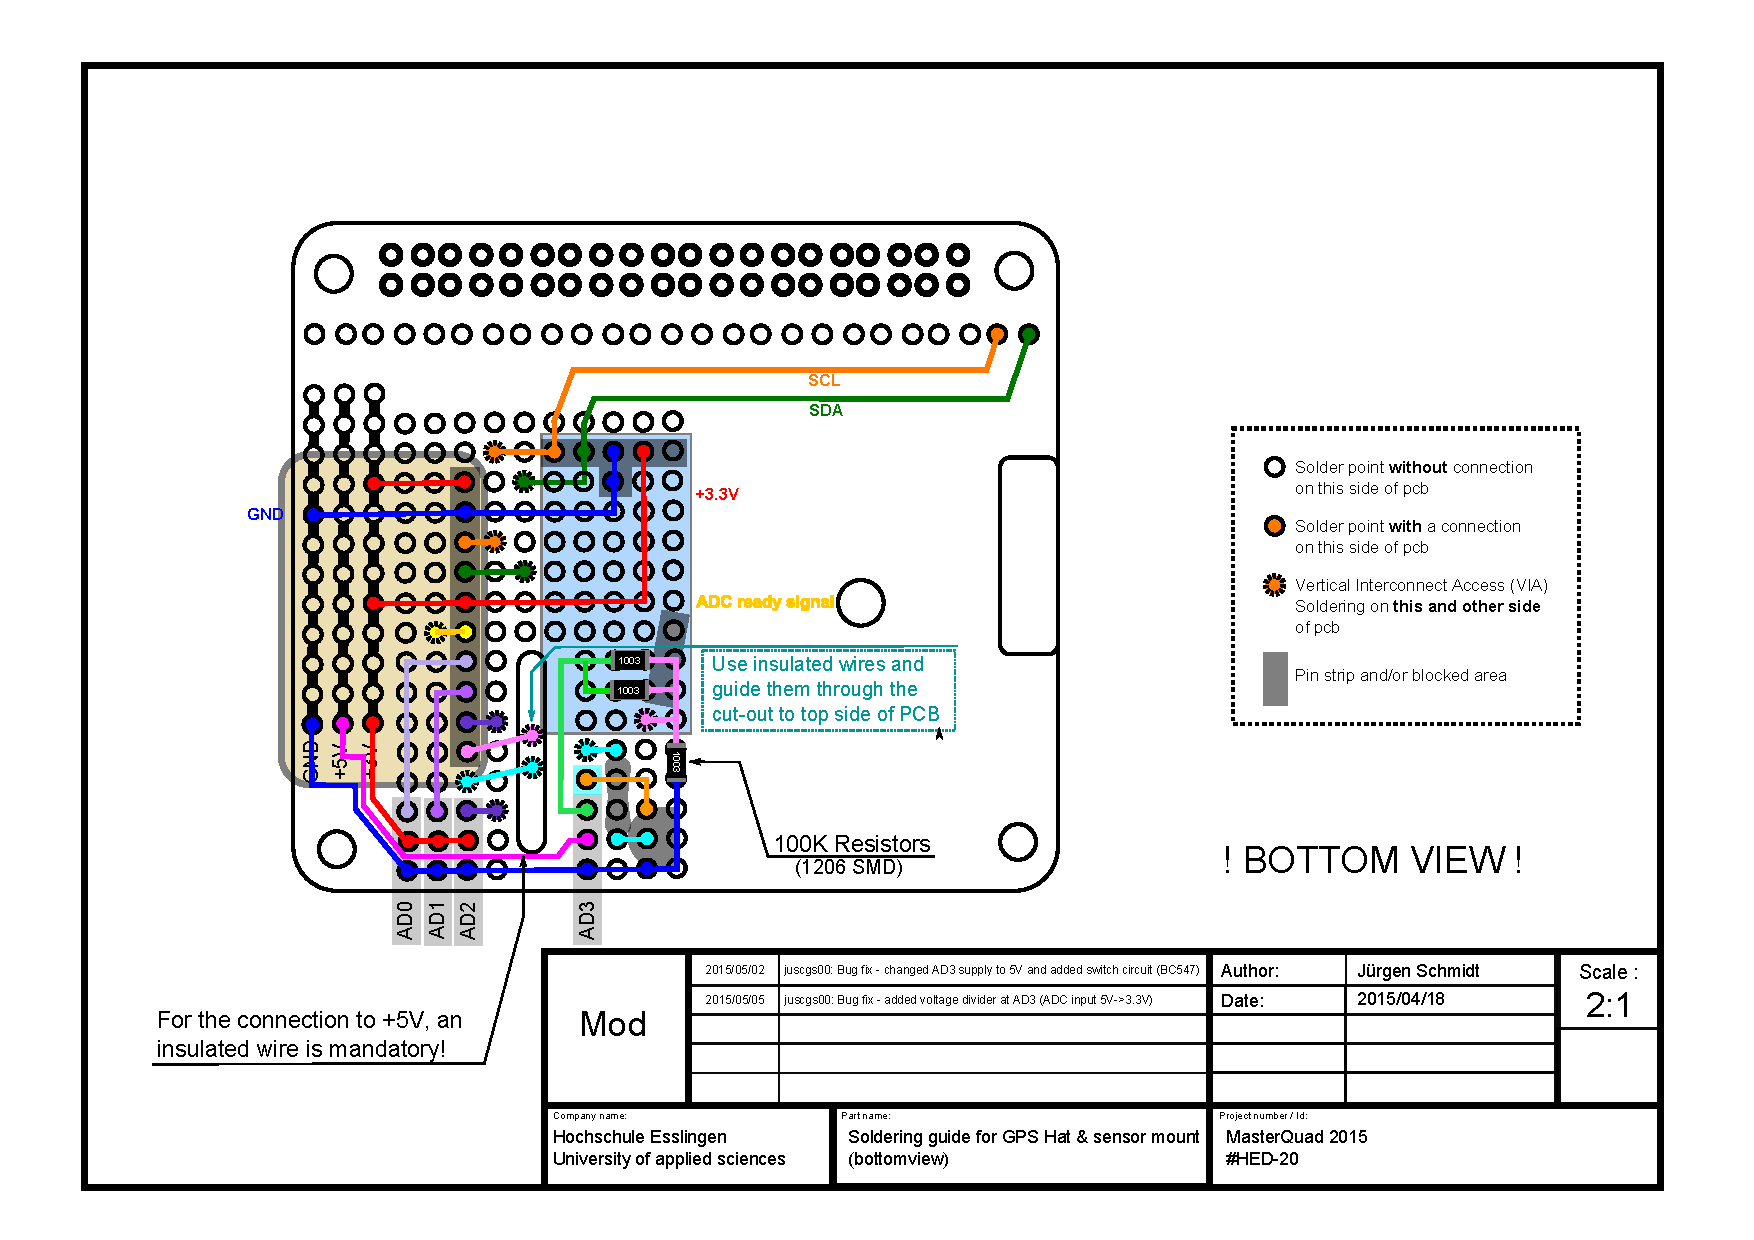
\includegraphics[width=0.87\textwidth]{fig/ch-rpi-hardware/A4_tech_draw_bottomview_gpshat_soldering}
    \caption{Soldering plan for Raspberry Pi Hat (bottom view)}
    \label{fig:hardware:soldering:bottom}
\end{figure}

\begin{figure}[H]
    \centering
    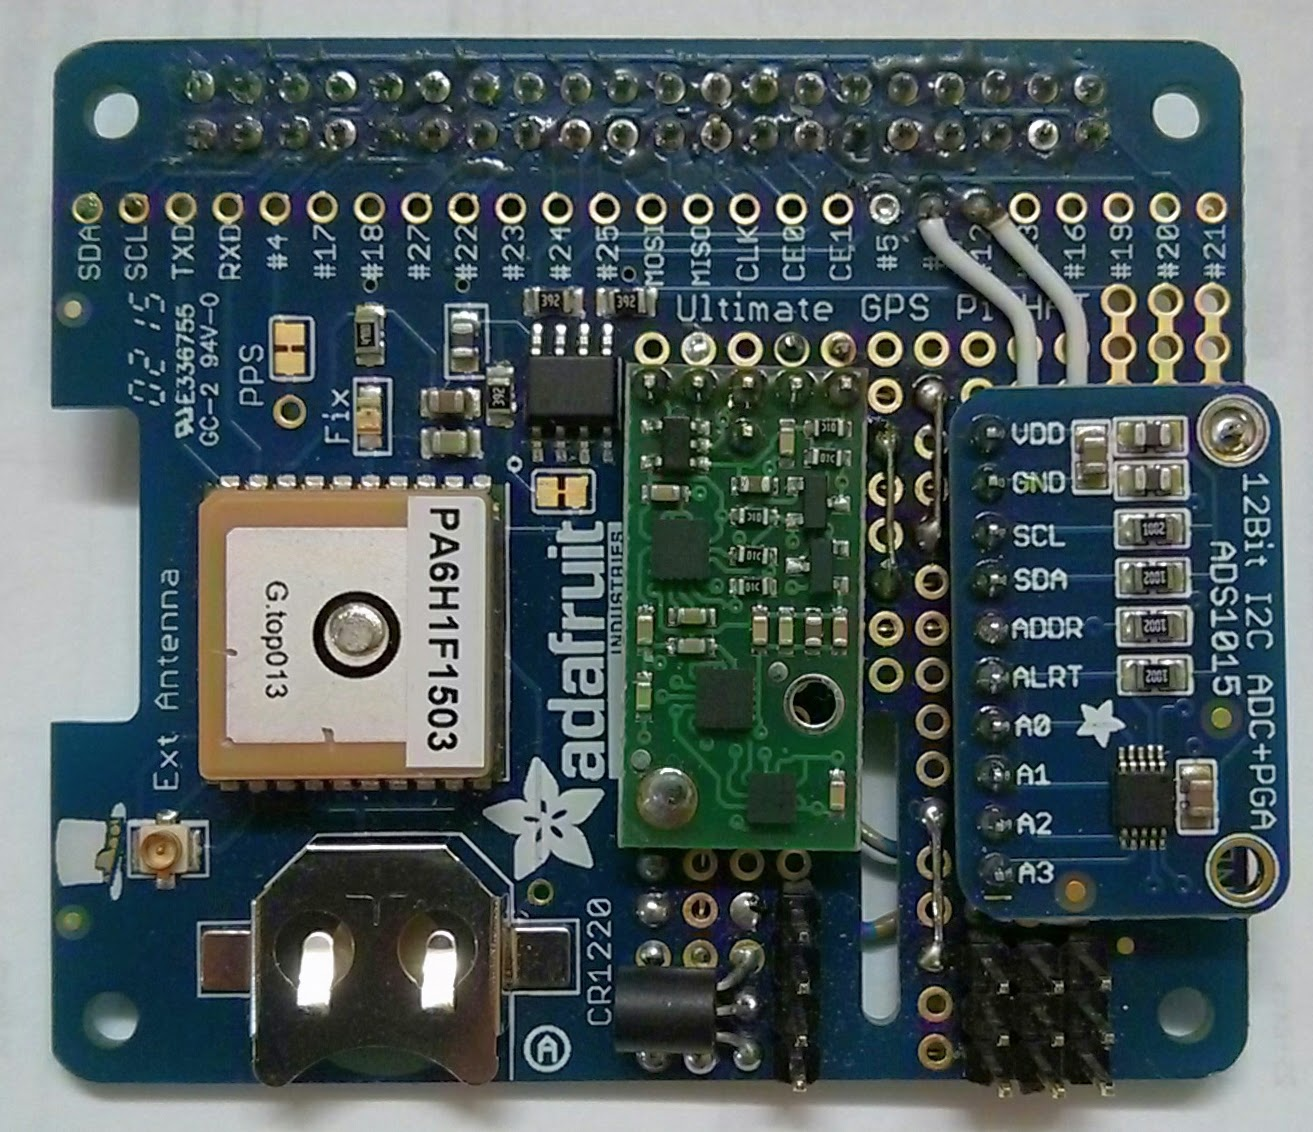
\includegraphics[width=0.71\textwidth]{fig/ch-rpi-hardware/picHatTop}
    \caption{Soldered Raspberry Pi Hat (top view)}
    \label{fig:hardware:mountedHat:top}
\end{figure}

\begin{figure}[H]
    \centering
    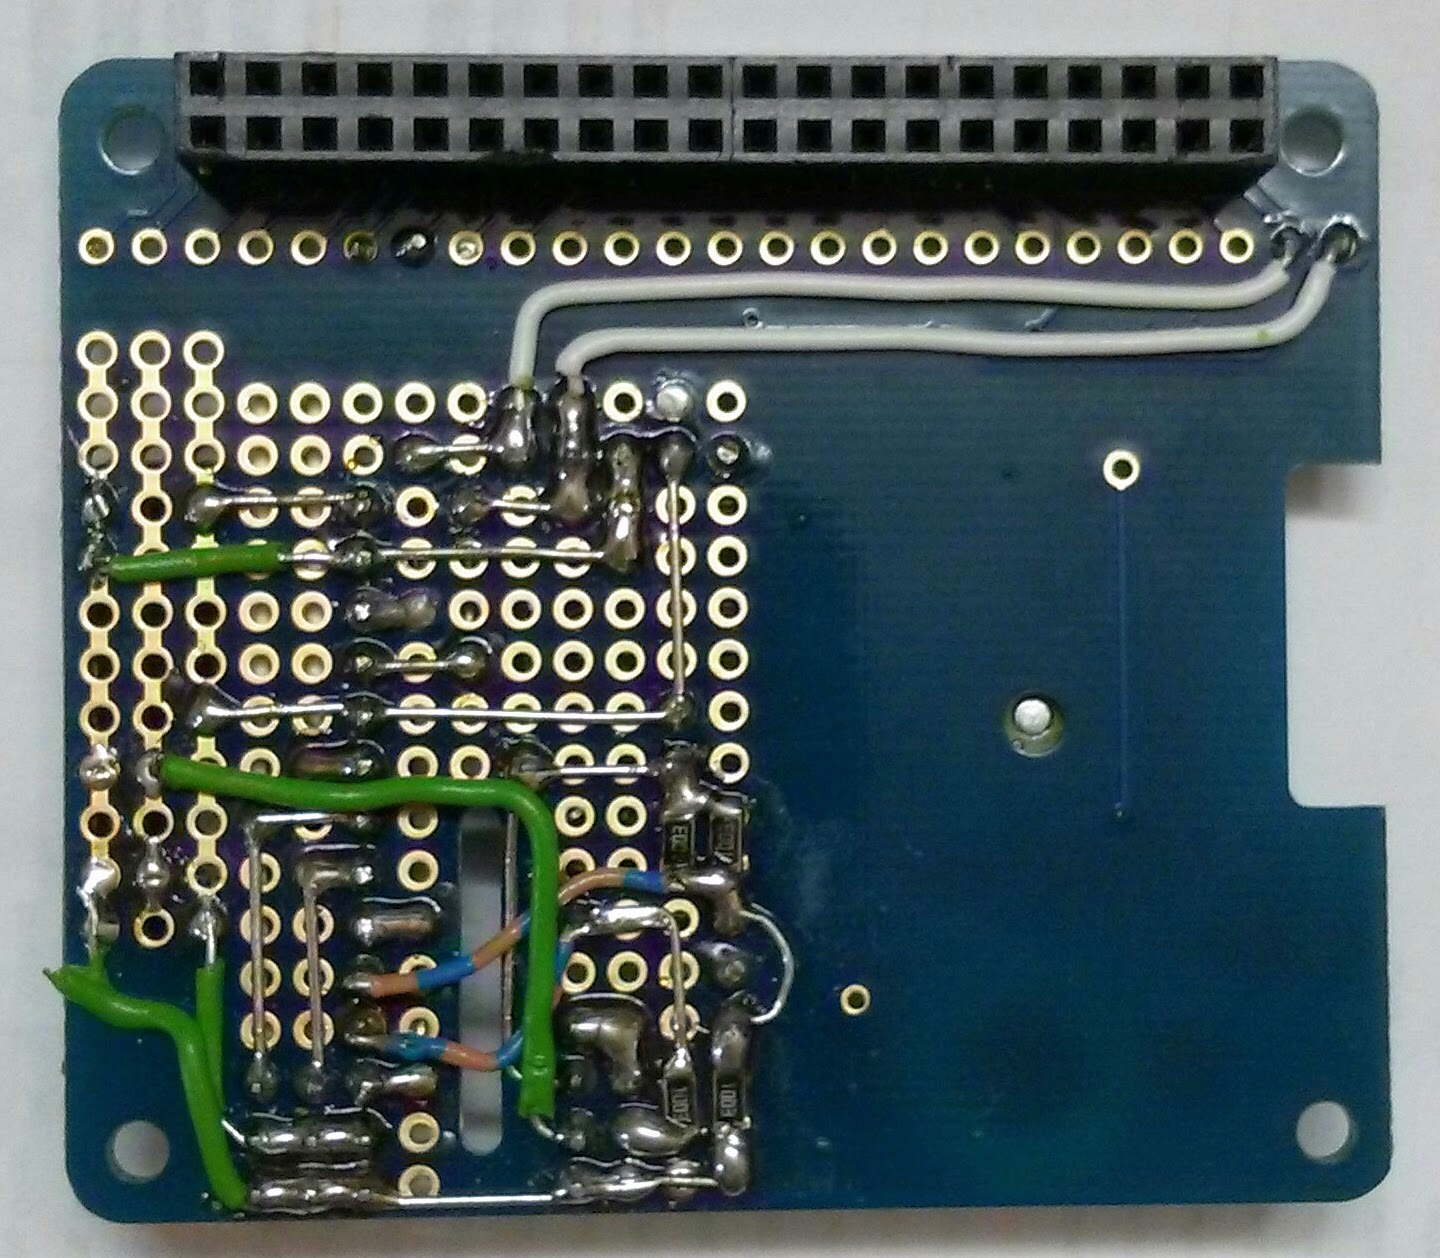
\includegraphics[width=0.71\textwidth]{fig/ch-rpi-hardware/picHatBottom}
    \caption{Soldered Raspberry Pi Hat (bottom view)}
    \label{fig:hardware:mountedHat:bottom}
\end{figure}

%- - - - - - - - - - - - - - - - - - - - - - 
% Section: Bill of materials
%- - - - - - - - - - - - - - - - - - - - - - 
\newpage
\section{Bill of materials}
\label{sec:hardware:BillOfMat}

For this project, the parts nedded for the Raspberry Pi Platform has been ordered 5 times. The following Bill of Materials lists all parts including the distributor and parts numbers.

\begin{figure}[H]
    \centering
    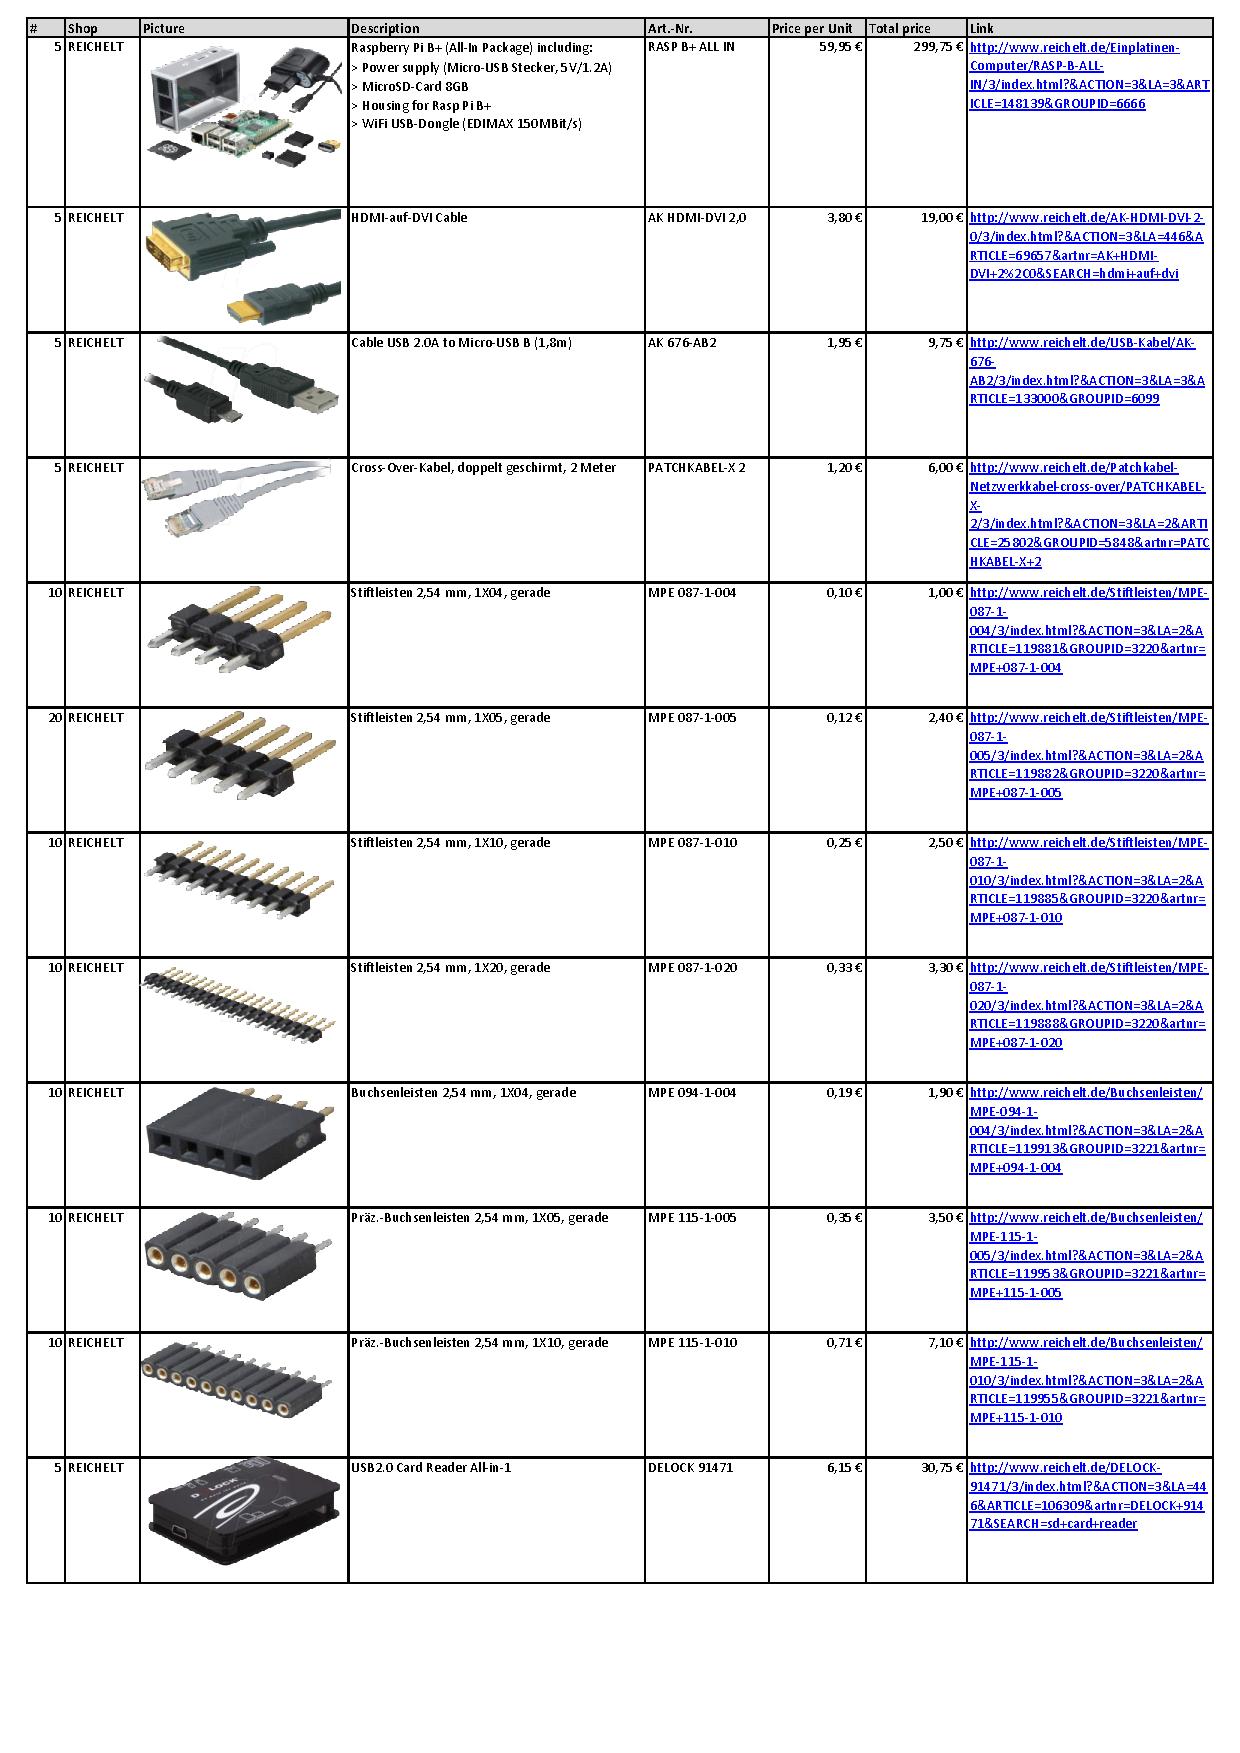
\includegraphics[width=0.90\textwidth,trim=0 80 0 8,clip=true]{fig/ch-rpi-hardware/1_Masterquad2015_BoM}
    \caption{Bill of materials, part 1}
    \label{fig:hardware:BillOfMat:1}
\end{figure}

\begin{figure}[H]
    \centering
    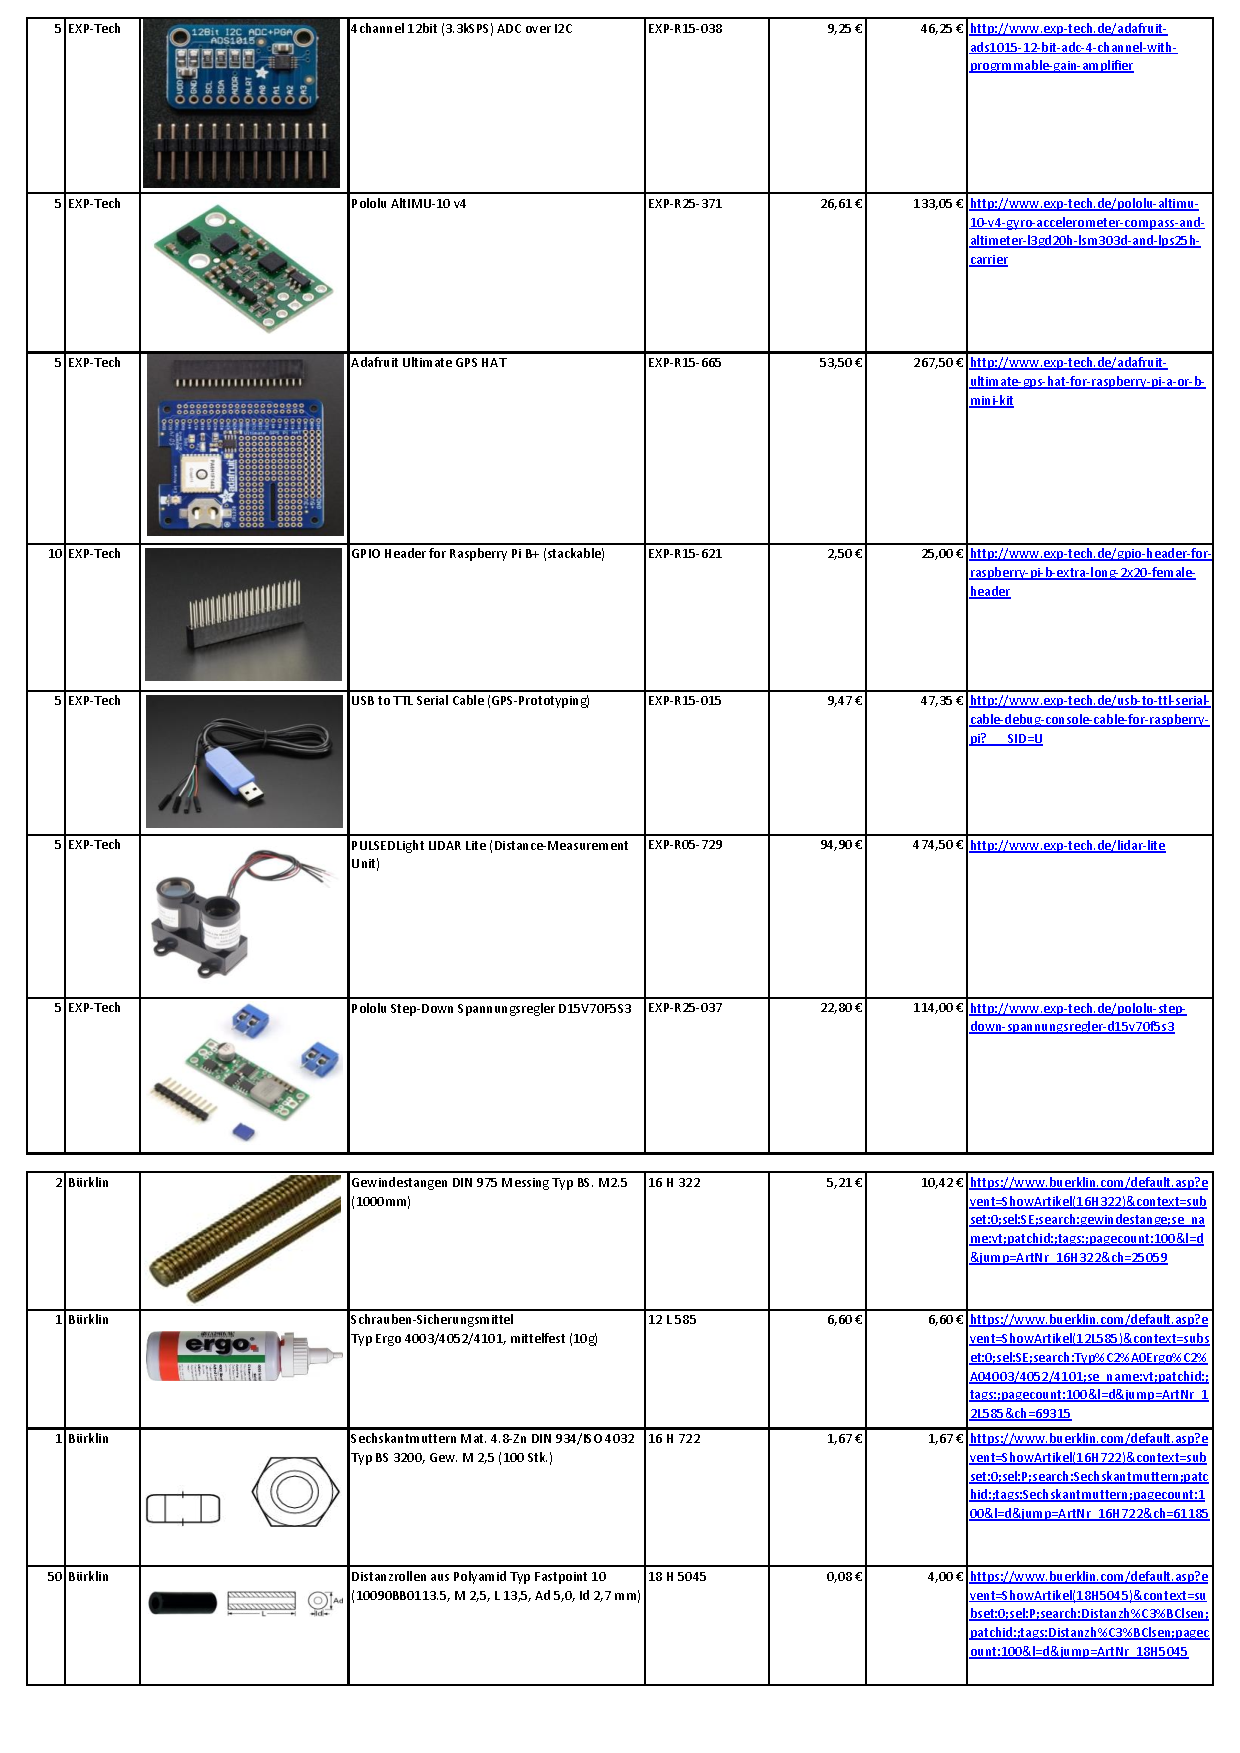
\includegraphics[width=0.97\textwidth,trim=0 31 0 8,clip=true]{fig/ch-rpi-hardware/2_Masterquad2015_BoM}
    \caption{Bill of materials, part 2}
    \label{fig:hardware:BillOfMat:2}
\end{figure}

\begin{figure}[H]
    \centering
    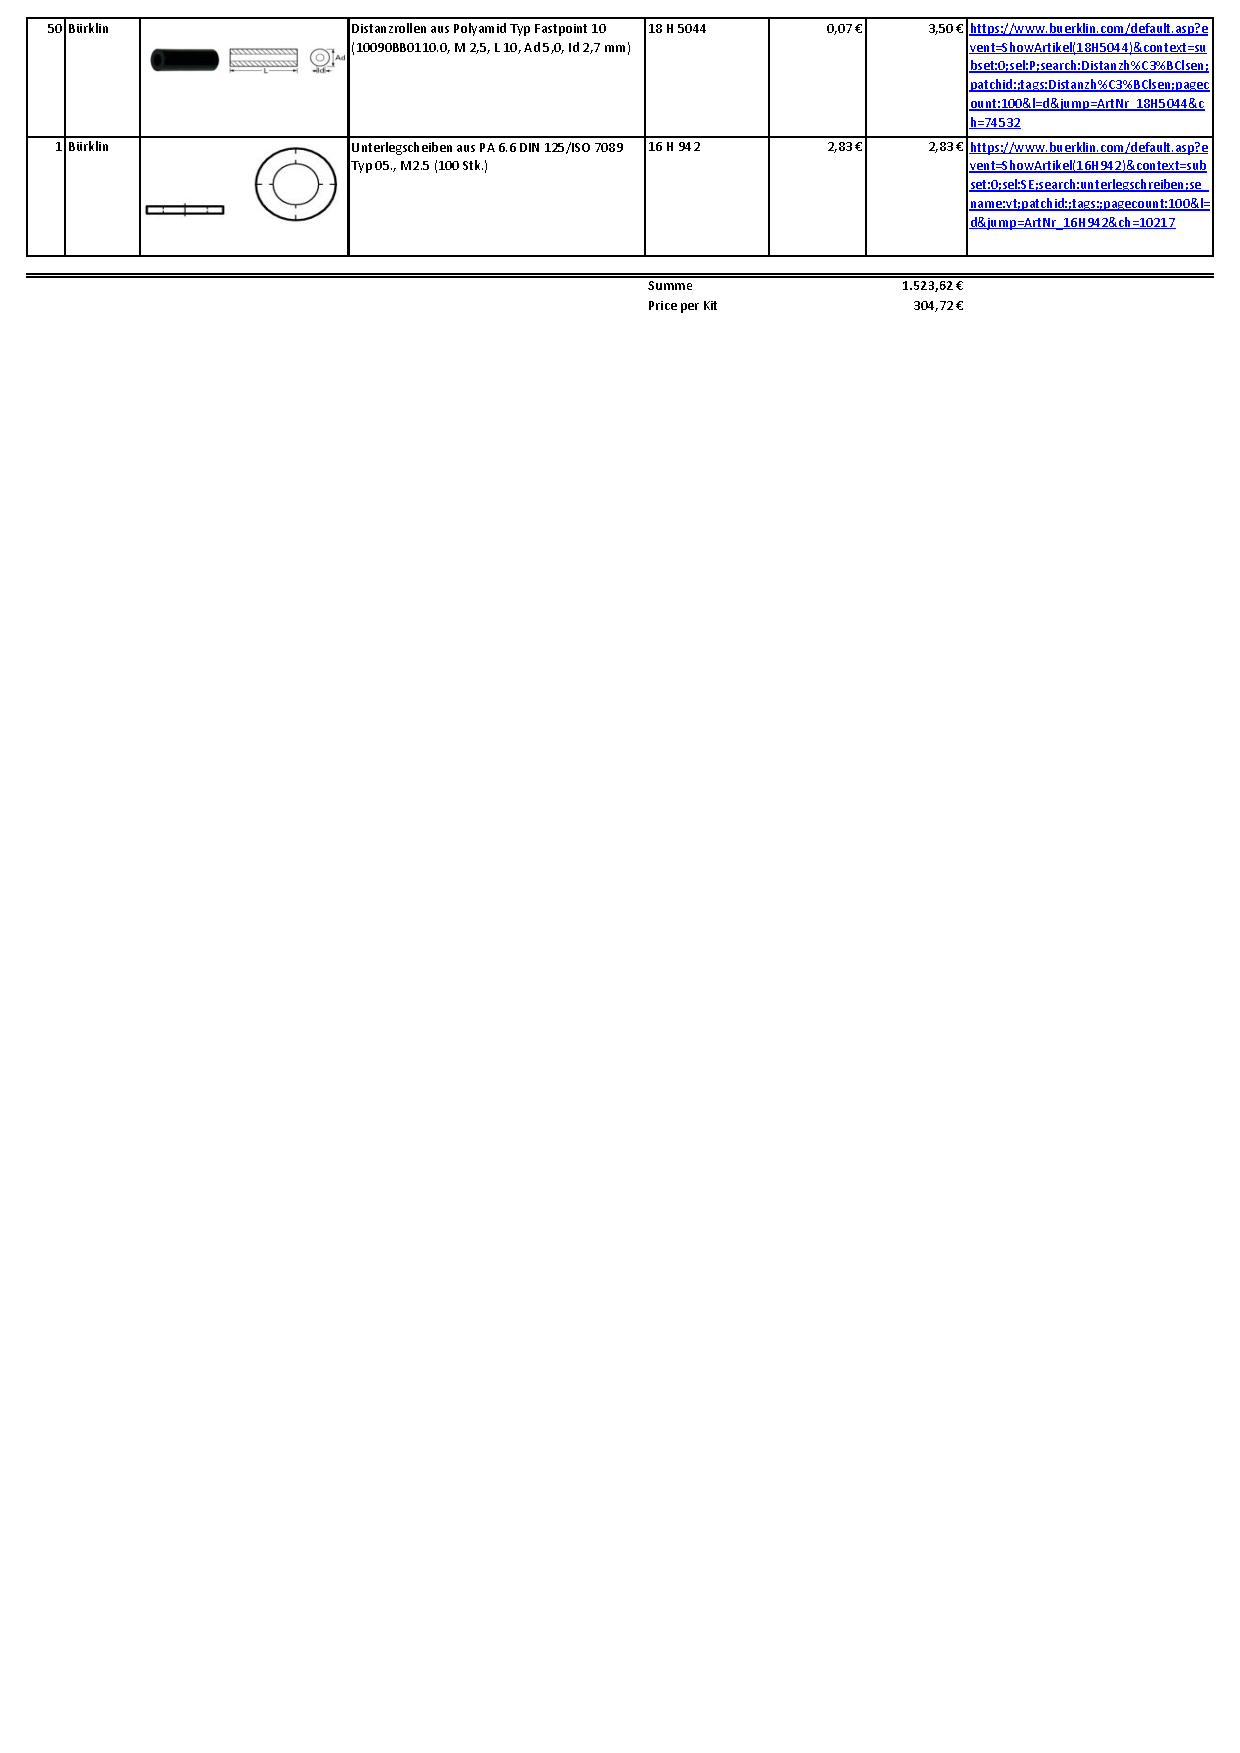
\includegraphics[trim=0 690 0 8,clip=true,width=0.97\textwidth]{fig/ch-rpi-hardware/3_Masterquad2015_BoM}
    \caption{Bill of materials, part 3}
    \label{fig:hardware:BillOfMat:3}
\end{figure}

\chapter{Individual parts}
\label{sec:parts}

\section{Raspberry Pi B+}
\label{sec:goals:rpib}
\begin{figure}[H]
    \centering
    
\includegraphics[width=\textwidth]{fig/ch-rpi-hardware/A4_tech_draw_topview_rpi}
    \caption{Raspberry Pi B+ (topview)}
    \label{fig:parts:rpi_topview}
\end{figure}

\newpage
\section{Adafruit GPS Hat}
\label{sec:goals:gpshat}
\begin{figure}[H]
    \centering
    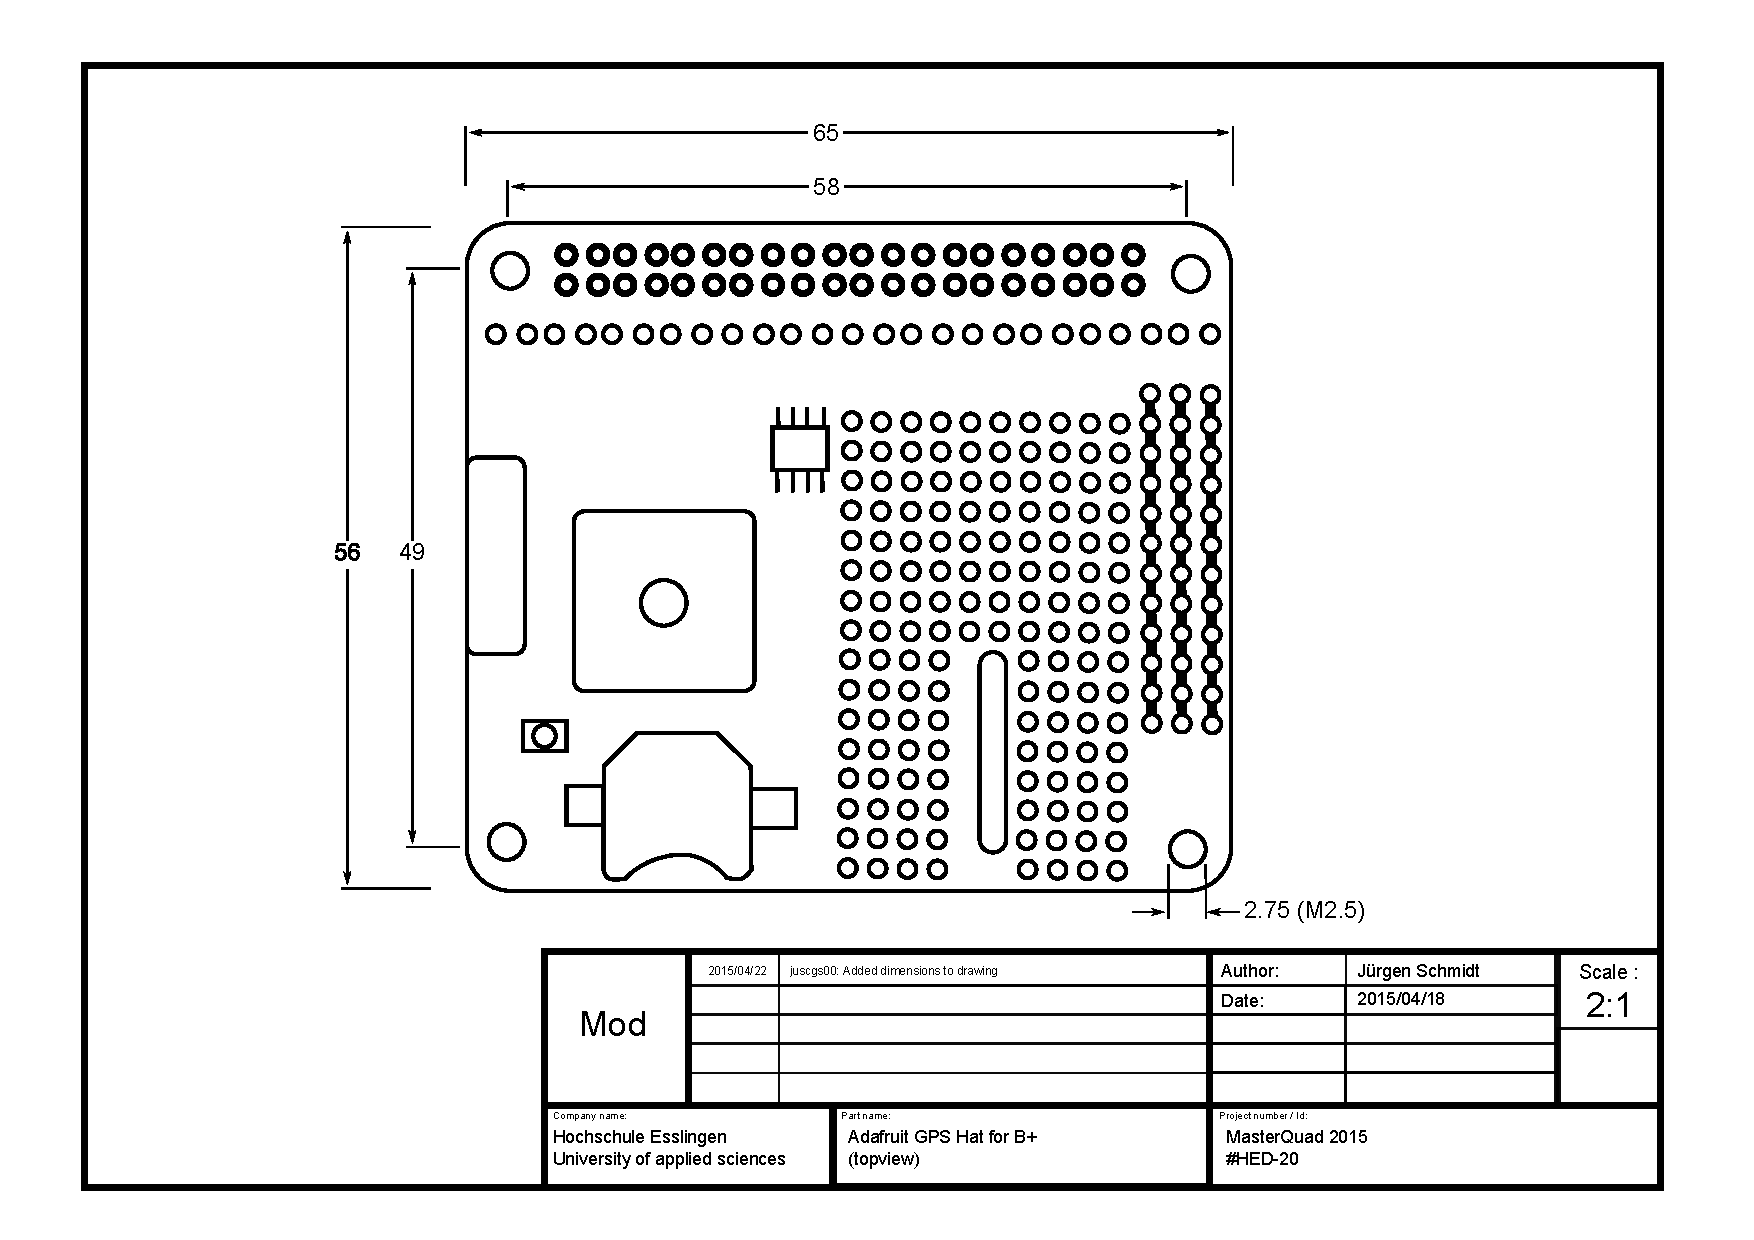
\includegraphics[width=\textwidth]{fig/ch-rpi-hardware/A4_tech_draw_topview_gpshat}
    \caption{Adafruit GPS Hat}
    \label{fig:parts:gps_topview}
\end{figure}

\newpage
\section{Polulu AltIMU v4}
\label{sec:goals:altimu}
\begin{figure}[H]
    \centering
    
\includegraphics[width=\textwidth]{fig/ch-rpi-hardware/A4_tech_draw_topview_imu}
    \caption{Polulu AltIMU v4}
    \label{fig:parts:imu_topview}
\end{figure}

\newpage
\section{Adafruit 12bit ADC over I2C}
\label{sec:goals:adc}
\begin{figure}[H]
    \centering
    
\includegraphics[width=\textwidth]{fig/ch-rpi-hardware/A4_tech_draw_topview_adc}
    \caption{Adafruit 12bit ADC over I2C}
    \label{fig:parts:adc_topview}
\end{figure}

%--------------------------------------------
% Chapter: ASSEMBLY
%--------------------------------------------
\chapter{Assembly}
\label{sec:assemb}

\section{Placing ADC and IMU on GPS Hat}
\label{sec:assemb:sensorsOnHat}
\begin{figure}[H]
    \centering
    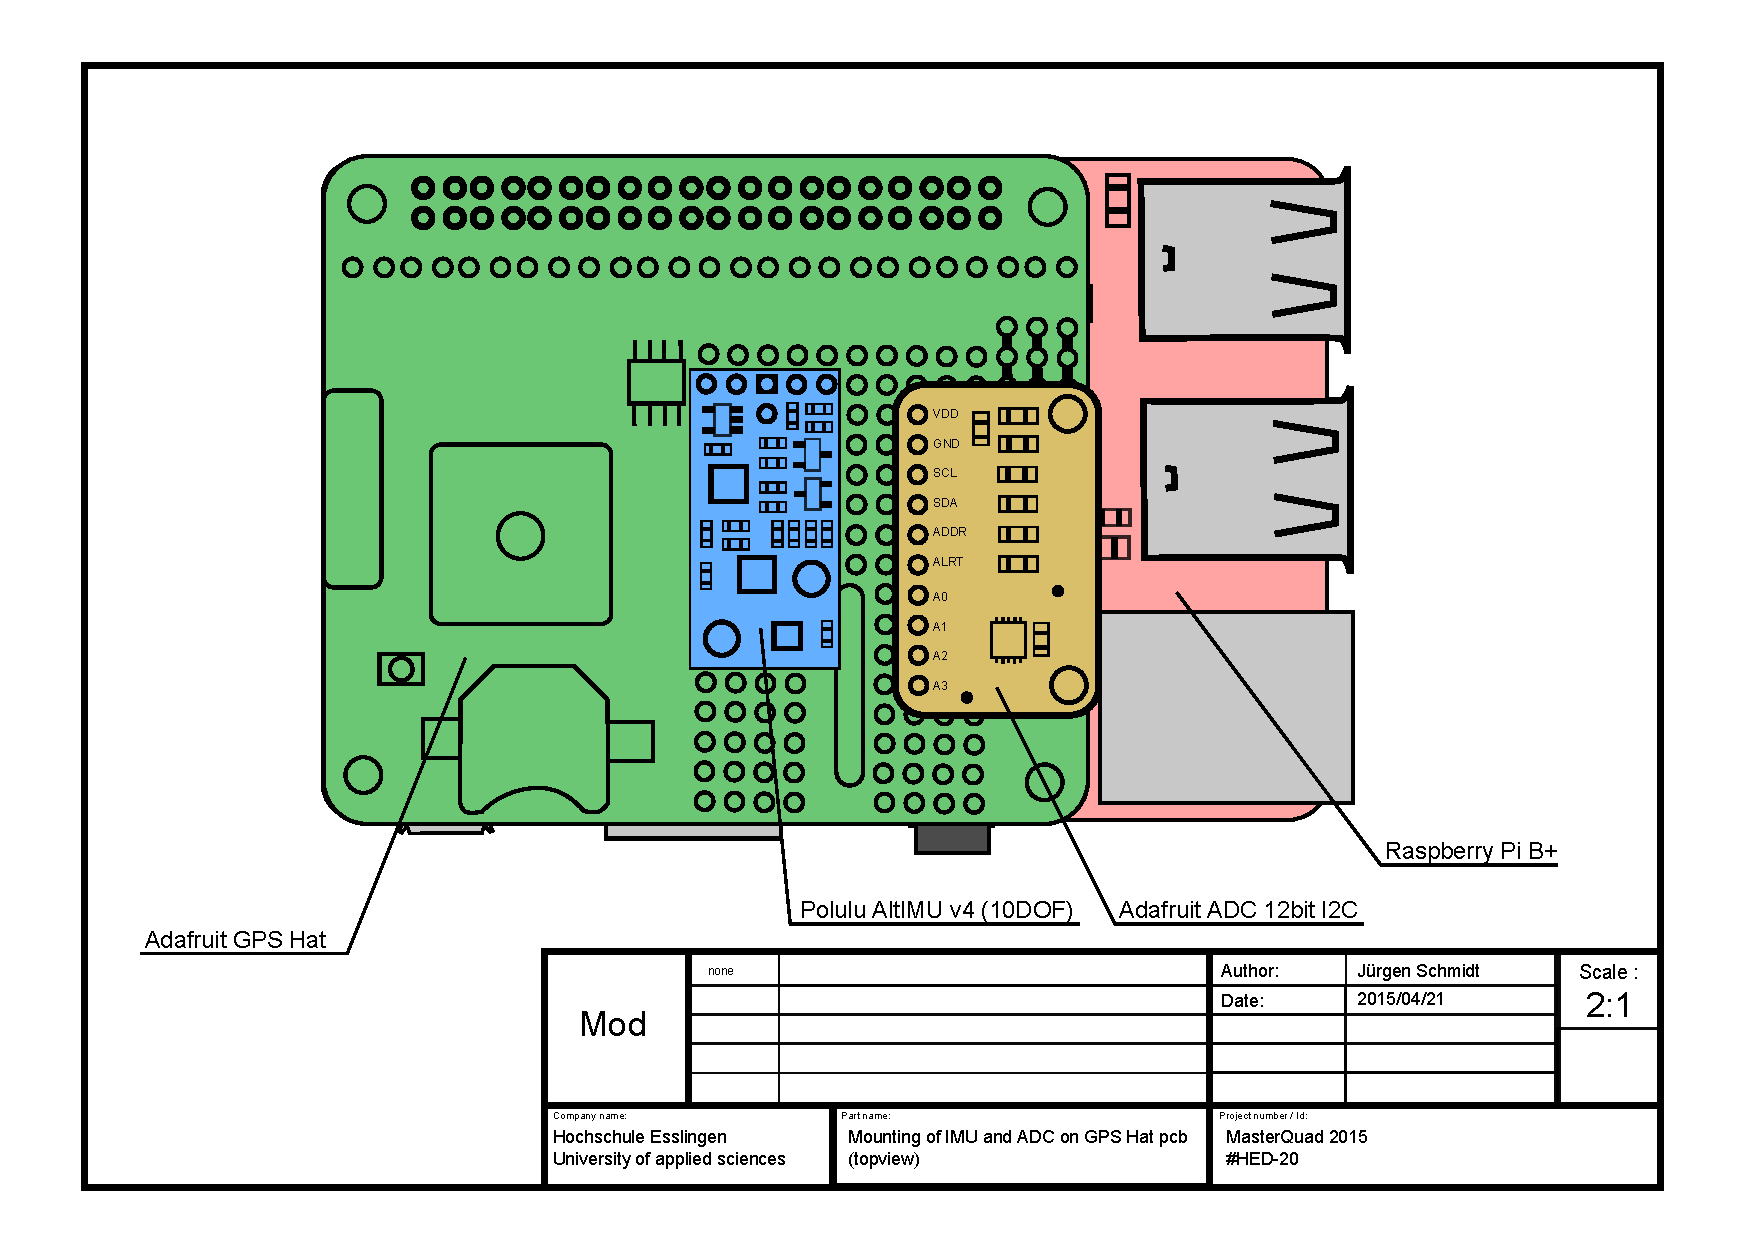
\includegraphics[width=\textwidth]{fig/ch-rpi-hardware/A4_tech_draw_topview_sensor_mountingPositions}
    \caption{Placing ADC and IMU on GPS Hat}
    \label{fig:assemb:sensorMount}
\end{figure}

\section{Wedding of GPS Hat and Raspberry Pi B+}
\label{sec:assemb:wedding}

%% Development Environment (Virtual Machine Image)
%--------------------------------------------
% Chapter: DEVELOPMENT ENVIRONMENT
%--------------------------------------------
\chapter{Development Environment (Virtual Machine Image and Native Machine)}
\label{sec:sec-VM}

This project uses the VMWare player of the company VMWare \footnote{https://my.vmware.com/de/web/vmware/free\#desktop\_end\_user\_computing/vmware\_player/7\_0}. This gives the ability that no dependency to a special operating system exists. It can run on any system like mac, windows or linux. A pre defined Image for the VMWare player can be found in the SVN repository folder \texttt{/sys/VM/}.
The native machine is based on 14.04 AMD64 Ubuntu.
If you have native machine and running the program there, then please directly skip to 
the section \textbf{Toolchain}

\begin{figure}[H]
	\centering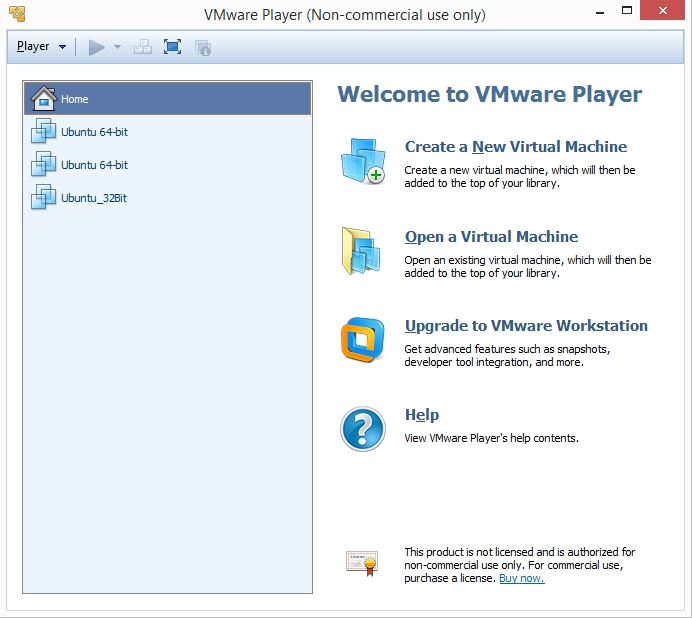
\includegraphics[width=0.5\textwidth]{fig/Dev_Concept/VMPlayer.jpg}
	\caption{VMWare Player}
	\label{fig:VMPlayer}
\end{figure}

\section{Ubuntu}
\label{subsec:sec-Ub}

Here the current Ubuntu 14.10 which is installed with the help of the VMWare player is used. For programming the software eclipse is taken. First the current image of Ubuntu needs to be downloaded:
\begin{lstlisting}
http://www.ubuntu.com/download
\end{lstlisting}
Figure \ref{fig:Ub1} shows the the window of the VMWare player directly after starting. To add a new virtual machine a click on 'Create a New Virtual Machine' has to be made.

\begin{figure}[H]
	\centering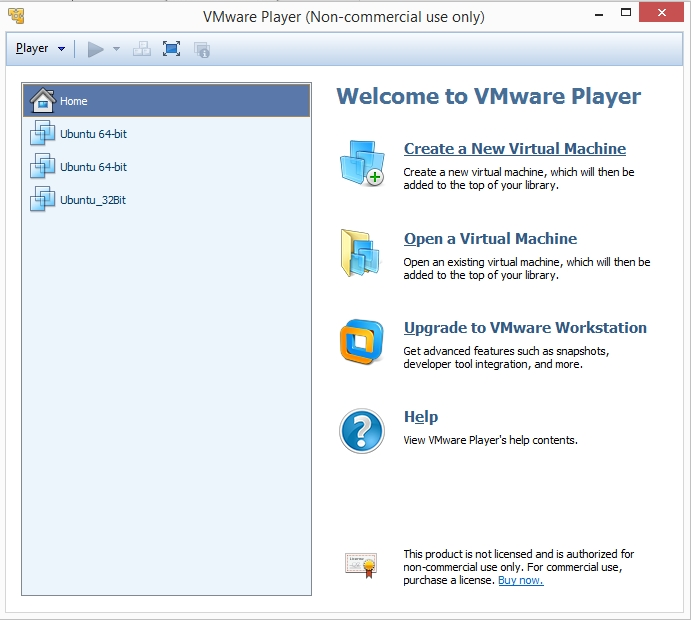
\includegraphics[width=0.4\textwidth]{fig/Dev_Concept/Ub1.jpg}
	\caption{Installing Ubuntu - Step 1: Create new virtual machine}
	\label{fig:Ub1}
\end{figure}

Then under the 'Installer disc image file (iso)', the path to the before downloaded ISO-file needs to be set like in the figure \ref{fig:Ub2}.

\begin{figure}[H]
	\centering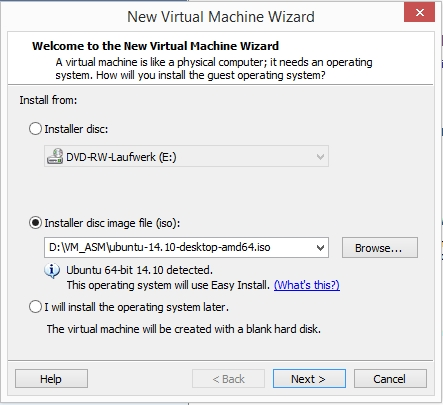
\includegraphics[width=0.4\textwidth]{fig/Dev_Concept/Ub2.jpg}
	\caption{Installing Ubuntu - Step 2: Installer ISO-file}
	\label{fig:Ub2}
\end{figure}

Figure \ref{fig:Ub3} shows the next step. A full name, a user and a password is set. In this project 'user' with password 'user' is used.

\begin{figure}[H]
	\centering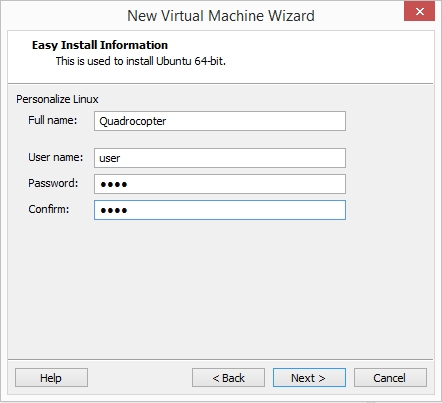
\includegraphics[width=0.5\textwidth]{fig/Dev_Concept/Ub3.jpg}
	\caption{Installing Ubuntu - Step 3: Setting up a generic user}
	\label{fig:Ub3}
\end{figure}

Then a name for the virtual machine and the location, where the virtual machine is stored is chosen. See figure \ref{fig:Ub4}.

\begin{figure}[H]
	\centering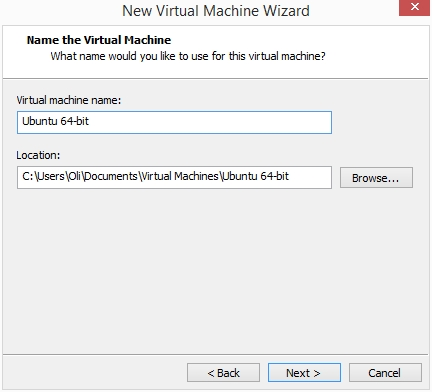
\includegraphics[width=0.5\textwidth]{fig/Dev_Concept/Ub4.jpg}
	\caption{Installing Ubuntu - Step 4: Name of virtual machine}
	\label{fig:Ub4}
\end{figure}

The following figures \ref{fig:Ub5} and \ref{fig:Ub6} show the option for the size and the splitting and finally a summary.

\begin{figure}[H]
	\centering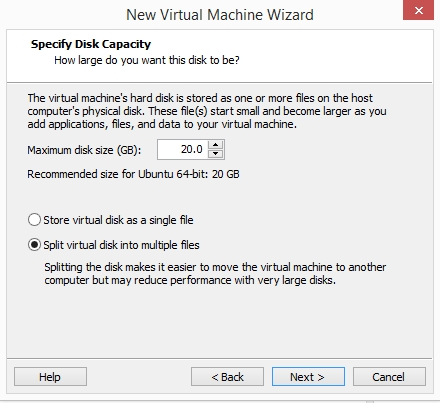
\includegraphics[width=0.5\textwidth]{fig/Dev_Concept/Ub5.jpg}
	\caption{Installing Ubuntu - Step 5: Choosing virtual disk size}
	\label{fig:Ub5}
\end{figure}

\begin{figure}[H]
	\centering\includegraphics[width=0.5\textwidth]{fig/Dev_Concept/Ub6.jpg}
	\caption{Installing Ubuntu - Step 6: Finalize virtual machine}
	\label{fig:Ub6}
\end{figure}

Then VMWare tools wants to be installed. This tool is needed for example to enable dynamic rescaling of the Desktop of Ubuntu within the VMWare player, so it should be installed. See figure \ref{fig:Ub7}.

\begin{figure}[H]
	\centering\includegraphics[width=0.5\textwidth]{fig/Dev_Concept/Ub7.jpg}
	\caption{Installing Ubuntu - Step 7: Installation of VMWare Tools}
	\label{fig:Ub7}
\end{figure}

Finally the login window of Ubuntu (figure \ref{fig:Ub9}).

\begin{figure}[H]
	\centering\includegraphics[width=0.5\textwidth]{fig/Dev_Concept/Ub9.jpg}
	\caption{Installing Ubuntu - Step 8: Ubuntu's system login}
	\label{fig:Ub9}
\end{figure}

Remark:\\
If the rescaling later on will not work, then after the start and login into Ubuntu, the following command needs to run in the terminal window:
\begin{lstlisting}[language=bash,otherkeywords={sudo,tar,touch,gedit,cp,apt-get,mkdir}]
sudo apt-get install open-vm-tools-desktop
\end{lstlisting}


\section{Toolchain}
\label{subsec:sec-TC}

A Toolchain enables compilation on the fast development computer instead on the Raspberry Pi. This is called cross compiling. To make it possible, following commands have to be called in the Ubuntu operating system which is running in the virtual machine. This description is based on the blog entry from Halherta \footnote{http://hertaville.com/2012/09/28/development-environment-raspberry-pi-cross-compiler/}.\\
First the cross compiling toolchain will be downloaded and set up. The following commands will be called in a terminal window.\\
The following command downloads the native build tools and the GIT tool which will be used to download the cross compiling toolchain.
\begin{lstlisting}[language=bash,otherkeywords={sudo,tar,touch,gedit,cp,apt-get,mkdir}]
sudo apt-get install build-essential git
\end{lstlisting}
Next a directory is created and then the directory is opened.
\begin{lstlisting}[language=bash,otherkeywords={sudo,tar,touch,gedit,cp,apt-get,mkdir}]
mkdir rpi
cd rpi
git clone git://github.com/raspberrypi/tools.git
\end{lstlisting}
The last command downloads the official cross compiling Toolchain. 
In the folder \newline/home/user/rpi/tools/arm-bcm2708 are now four different folders stored which contain different toolchains.
\begin{lstlisting}[language=bash]
 arm-bcm2708-linux-gnueabi
 arm-bcm2708hardfp-linux-gnueabi
 gcc-linaro-arm-linux-gnueabihf-raspbian
 gcc-linaro-arm-linux-gnueabihf-raspbian-x64
\end{lstlisting}
Due to the reason that the used Ubuntu is a 64 bit OS the fourth toolchain has to be used.
To enable compilation also directly from the command line, the path to the Toolchain has to be added in the PATH variable of the Ubuntu system. To do so, the following actions need to be done.

\begin{lstlisting}[language=bash,otherkeywords={sudo,tar,touch,gedit,cp,apt-get,mkdir},escapechar=|]
cd ~/
nano .bashrc
export PATH=$PATH:$HOME/rpi/tools/arm-bcm2708/|\\|gcc-linaro-arm-linux-gnueabihf-raspbian-x64/bin
source .bashrc
\end{lstlisting}
The last command updats the PATH variable.\\
If all actions are successfully done, it can be proved by:
\begin{lstlisting}[language=bash]
arm-linux-gnueabihf-gcc -v
\end{lstlisting}
If all works fine the terminal window should show following output.

\begin{figure}[H]
	\centering\includegraphics[width=1\textwidth]{fig/Dev_Concept/Cross_compile_success.jpg}
	\caption{Prove of successfull working Toolchain}
	\label{fig:Cross_compile_success}
\end{figure}

\section{Eclipse}
\label{subsec:subsec-Eclipse-header}

\subsection{Installation of Eclipse Luna}
\label{subsec:subsec-Eclipse}

Next, the current 64 Bit Eclipse IDE for C/C++ Developers, is downloaded from the webpage of eclipse within the Ubuntu system:
\begin{lstlisting}
https://www.eclipse.org/downloads/?osType=linux
\end{lstlisting}

First the current Java runtime environment is installed.
\begin{lstlisting}[language=bash,otherkeywords={sudo,tar,touch,gedit,cp,apt-get,mkdir}]
sudo apt-get install openjdk-7-jre
\end{lstlisting}
Then the before downloaded eclipse is extracted and stored to /opt
\begin{lstlisting}[language=bash,otherkeywords={sudo,tar,touch,gedit,apt-get,mkdir}]
sudo tar -xvzf eclipse-cpp-luna-SR2-linux-gtk-x86_64 -C /opt/
\end{lstlisting}
In order to access the most recent eclipse, a custom desktop link has to be created and edited. 
\begin{lstlisting}[language=bash,otherkeywords={sudo,tar,touch,gedit,cp,apt-get,mkdir}]
sudo touch /usr/share/applications/eclipse-recent.desktop;
sudo gedit /usr/share/applications/eclipse-recent.desktop &
\end{lstlisting}
An editor will open after executing the above shown lines. Paste the following lines in order to create a valid Ubuntu desktop launcher:
\begin{lstlisting}
[Desktop Entry]
Type=Application
Name=Eclipse Luna
Comment=Eclipse Integrated Development Environment
Icon=/opt/eclipse/icon.xpm
Exec=/opt/eclipse/eclipse
Terminal=false
Categories=Development;IDE;Java;
\end{lstlisting}

Optionally, a starter icon can be put to the desktop of Ubuntu by copying the above created Ubuntu desktop launcher:
\begin{lstlisting}[language=bash,otherkeywords={sudo,cp,apt-get,mkdir}]
sudo cp /usr/share/applications/eclipse-recent.desktop ~/Desktop/
\end{lstlisting}

\subsection{Remote Debugging}
\label{subsubsec:subsubsec-RD}

Enabling remote debugging is really helpfull when a written program has not the  expected behaviour. To enable remote debugging, some configurations in the Debug Configurations need to be done. This window can be found under 'Run/Debug Configurations...'
In the starting window a click with the left mousebutton on 'C/C++ Remote Application' on the left part of the window needs to be done. Then click on 'New'. See figure \ref{fig:Debug1}.

\begin{figure}[H]
	\centering\includegraphics[width=0.7\textwidth]{fig/Dev_Concept/Debug1}
	\caption{Making new Debug Configuration}
	\label{fig:Debug1}
\end{figure}

In the appearing window write down first the Name 'Automatic\_Debug' and then in the tab 'Main' (see figure \ref{fig:Debug2}) write down the name of the project in the textfield 'Project:' and in 'C/C++ Application:' the executable, the binary file, which is in the Debug folder of the project. Under 'Build configuration' 'Use Active' and the radio button 'Enable auto build' has to be activated. When clicking under 'Connection:' on 'New...' a new window, like in figure \ref{fig:Debug3} appears. Here 'SSH only' and 'Next>' needs to be clicked. After that, in the next automatically popped up window all what needs to be written down can be seen in figure \ref{fig:Debug4}, and then it has to be confirmed by clicking on 'OK'. Last but not least there needs to be set a Folder which can be a existing or a new one in 'Remote Absolute File Path for C/C++ Application:' and under 'Commands to execute before application' the commands
\begin{lstlisting}[language=bash]
sudo -i
chmod +x Raspberry_Template
\end{lstlisting}
have to be included. Last make sure that in the lower area of the window 'Using GDB (DSF) Automatic Remote Debugging Launcher' is active.

\begin{figure}[H]
	\centering\includegraphics[width=0.9\textwidth]{fig/Dev_Concept/Debug2}
	\caption{Debug Configuration Window - Main tab}
	\label{fig:Debug2}
\end{figure}

\begin{figure}[H]
	\centering\includegraphics[width=0.5\textwidth]{fig/Dev_Concept/Debug3}
	\caption{Creating new connection 1}
	\label{fig:Debug3}
\end{figure}

\begin{figure}[H]
	\centering\includegraphics[width=0.7\textwidth]{fig/Dev_Concept/Debug4}
	\caption{Creating new connection 2}
	\label{fig:Debug4}
\end{figure}

\begin{figure}[H]
	\centering\includegraphics[width=0.9\textwidth]{fig/Dev_Concept/Debug6}
	\caption{Debug Configuration Window - Debugger tab}
	\label{fig:Debug6}
\end{figure}
After this is finished, in the Debugger tab, there needs in the 'GDB debugger' textfield 'arm-linux-gnueabihf-gdb' written down. This ensures that the ARM toolchain connects to the GDB server on the Raspberry (See figure \ref{fig:Debug6}).

\begin{figure}[H]
	\centering\includegraphics[width=0.9\textwidth]{fig/Dev_Concept/Debug7}
	\caption{Debug Configuration Window - Common tab}
	\label{fig:Debug7}
\end{figure}

Then in the 'Common' tab in 'Display in favorites menu' the 'Debug' checkbox needs to be activated. After that the window can be closed. Now all necessary actions are done and an existing project can be by debugged by clicking on the small arrow beneath the the small bug in the menu bar. Here the before saved Configuration (Automatic\_Debug) has to be activated what the debugging directly starts.

\begin{figure}[H]
	\centering\includegraphics[width=0.9\textwidth]{fig/Dev_Concept/Debug8}
	\caption{Start Debugging}
	\label{fig:Debug8}
\end{figure}


%\subsection{Create project and start on the Raspberry}
%\label{subsubsec:subsubsec-eclipseproject}
%
%\workTodo{http://hertaville.com/2012/09/28/development-environment-raspberry-pi-cross-compiler/}








%% Realtime-capable Linux Operating System
%--------------------------------------------
% Chapter: LINUX OPERATING SYSTEM
%--------------------------------------------
\chapter{Realtime-capable Linux Operating System}
\label{sec:OS}

%- - - - - - - - - - - - - - - - - - - - - - 
% Section: Setting up a bootable SD-Card 
%					 with an Raspbian Distribution
%- - - - - - - - - - - - - - - - - - - - - - 
\section{Creating a bootable SD-Card with a pre-configured Firmware}
\label{sec:OS:sdCardSetup}

For a convenient and easy start with the Raspberry Pi, a pre-configured Raspberry Pi Firmware can be found at the SVN repository folder \texttt{/sys/RPi/}. The pre-configured Firmware Image is based on the EMLID-distribution (see also chapter \ref{sec:OS:emlid}). The EMLID-distribution originates from a open source project\footnote{EMLID-Distribution: \url{http://www.emlid.com/new-raspbian-with-real-time-kernel-jan-2015/}} for a different Raspberry Pi based Quadcopter. It comprises the RT-Kernel patch as well as several optimizations regarding the system configuration to access peripherals that fit to the needs of this project\footnote{The hardware setup as well as the software architecture was planned before the authors have discovered the EMLID-distribution. It was a lucky coincidence, that the EMLID-distribution met almost all core requirements of this project. Because of that, the authors could used the EMLID-distribution as a base distribution during the software development and could develop in parallel - independently from the progress of patching the Raspbian distribution to a RTOS (as shown in chapter \ref{sec:OS:preemptRtPatch}).}.

For this project, pick the archive file \texttt{EMLID\_Preempt\_IP192.168.2.1.zip} from the SVN repository. Unzip the file to get the extracted 8GB Firmware Image.

To write the Firmware Image to a SD Card, use the tool \texttt{Win32DiskImager}\footnote{Download \texttt{Win32DiskImager} at \url{http://sourceforge.net/projects/win32diskimager/}} for Windows based Host machines (as shown in fig. \ref{fig:OS:win32DiskImager}).
\begin{figure}[H]
    \centering
    \includegraphics[width=0.65\textwidth]{fig/ch-rt-linux-os/Win32DiskImager}
    \caption[Windows tool Win32DiskImager]{Windows tool Win32DiskImager to write a Raspberry Pi Firmware to a SD Card in a Windows Host System}
    \label{fig:OS:win32DiskImager}
\end{figure}

For Linux based host machines (as well as the Development Environment VM), the built-in program \texttt{dd} can be used to copy the Firmware to a SD card. Therefore, the device handler \texttt{/dev/sd}X has to be determined, first! Issue the command \texttt{lsblk} and search for a disk with the same size as the SD card.\\
Assuming the device handler is \texttt{/dev/sdb} (use device handler of complete disk, without any numbers in the name), the Firmware can be copied with the below shown command.

\textbf{Attention:}\\
A wrong chosen device handler can destroy the operating system of the host machine!
\begin{lstlisting}[language=bash,otherkeywords={unzip,dd,sudo,of}]
cd ../path/to/svnRepository/sys/RPi/
unzip EMLID_Preempt_IP192.168.2.1.zip
sudo dd if=EMLID_Preempt_192.168.2.1.img of=/dev/sdb
\end{lstlisting}

\textbf{Remark:}\\
To use the pre-configured Firmware Image, a SD Card with at least 8GB storage capacity has to be used! Otherwise, the Firmware Image will be too big.

%- - - - - - - - - - - - - - - - - - - - - - 
% Section: Patching Linux Kernel to PREEMPT_RT version
%- - - - - - - - - - - - - - - - - - - - - - 
\section[Building a Real-Time Linux Kernel]{Building a Real-Time Linux Kernel for the Raspberry Pi}
\label{sec:OS:preemptRtPatch}
In the following chapters, the folder structure for the kernel sources and kernel developments on the Development Environment (Virtual Machine) will be evolving such that the following folder structure appears:
\dirtree{%
.1 $\sim$/\DTcomment{Home-directory of the current user}.
.2 rpi\DTcomment{Raspberry Pi related sources and files}.
.3 linux\DTcomment{Linux Kernel sources}.
.3 linux-rt-rpi\DTcomment{EMLID-based Kernel sources (see chapter \ref{sec:OS:emlid})}.
.3 tools\DTcomment{Raspberry Pi toolchain tools}.
}
Therefore, first create the first folder hierarchy \texttt{rpi} with the commands
\begin{lstlisting}[language=bash,otherkeywords={mkdir,cd,dd,sudo}]
cd ~
mkdir rpi
cd rpi
\end{lstlisting}

Next, get latest RT-Kernel patch from the official website of the Linux Kernel Organization, Inc. (\url{https://www.kernel.org/pub/linux/kernel/projects/rt/}). Open the link with a browser in the Development Environment VM and navigate to the current stable release of Linux kernels (version 3.18 at the time of this project). Choose the file \texttt{patch-3.18.XX-rtXX.patch.xz} and copy the URL. Use the copied link to issue the command \texttt{wget} to download the Kernel patch archive into the folder \texttt{$\sim$/rpi/linux}, similar as shown below:
\begin{lstlisting}[language=bash,otherkeywords={mkdir,wget,xcat,dd,sudo}]
cd ~/rpi/
mkdir linux
cd linux
wget https://www.kernel.org/pub/linux/kernel/projects/rt/3.18/patch-3.18.16-rt13.patch.xz
\end{lstlisting}

As the RT-Kernel patch version and the kernel source version \textbf{must match}, the next step will be to get the Linux kernel source according to the latest available RT-patch version.\\
For that purpose, browse to \url{https://github.com/raspberrypi/linux/} to observe the available branches (see fig.\ref{fig:OS:preemptRtPatch:githubBrowser}). After a matching Kernel source branch could be determined, load the Kernel sources to the Development Environment using the command \texttt{git clone [URL]}. With the additional option \texttt{-b}, the corresponding branch can be chosen:
\begin{lstlisting}[language=bash,otherkeywords={cd,dd,sudo}]
cd ~/rpi/
git clone --depth=1 git://github.com/raspberrypi/linux.git -b rpi-3.18.y
\end{lstlisting}

The download of the kernel sources will take some time. According to the available bandwidth of the github servers, this may take even 1 - 2 hours!

\begin{figure}[H]
    \centering
    \includegraphics[width=0.85\textwidth]{fig/ch-rt-linux-os/githubBranchesBrowser}
    \caption[Branch list of github's Raspberry Pi Kernel sources]{Branch list of github's repository of the Raspberry Pi's Kernel sources}
    \label{fig:OS:preemptRtPatch:githubBrowser}
\end{figure}

Verify the downloaded kernel version by typing \texttt{make kernelversion} and check that the Kernel version number matches the Kernel version of the RT-Kernel patch.\\
Example:
\begin{lstlisting}[language=bash,otherkeywords={make, xcat,cd,dd,sudo}]
user@ubuntu:~/rpi$ cd linux
user@ubuntu:~/rpi/linux$ make kernelversion
3.18.16
\end{lstlisting}

If the Kernel version numbers match, the RT-Kernel patch can be applied to the Kernel sources. First, a dry run will be executed to check for errors:
\begin{lstlisting}[language=bash,otherkeywords={xcat,cd,dd,sudo}]
cd ~/rpi/linux/
xcat patch-3.18.16-rt13.patch.xz | patch -p 1 --dry-run
\end{lstlisting}

If no errors occur, the patch process can be applied without dry-run option:
\begin{lstlisting}[language=bash,otherkeywords={xcat,dd,sudo}]
xcat patch-3.18.16-rt13.patch.xz | patch -p 1
\end{lstlisting}

Now the Kernel sources have been patched to a Preempt\_RT setup! Next, the Kernel source have to get compiled. Therefore, the Raspberry Pi cross-compile toolchain has to be downloaded, if not already given (see also chapter \ref{sec:sec-VM} for details):
\begin{lstlisting}[language=bash,otherkeywords={dd,sudo}]
cd ~/rpi/
git clone --depth=1 git://github.com/raspberrypi/tools.git
\end{lstlisting}

The following compilation process shown in this documentation is based on the article of \cite{doc:Kern69}. In order to cross-compile the sources in the Development Environment VM, some environment variables in the command line have to be set up:
\begin{lstlisting}[language=bash,otherkeywords={sudo,export}]
export ARCH=arm
export CROSS_COMPILE=../tools/tools/arm-bcm2708/gcc-linaro-arm-linux-gnueabihf-raspbian-x64/bin/arm-linux-gnueabi-
export INSTALL_MOD_PATH=~/rpi/linux/outputLib
mkdir ~/rpi/linux/outputLib
\end{lstlisting}

Now, navigate to the sources and make Raspberry Pi configuration of the kernel sources.
\begin{lstlisting}[language=bash,otherkeywords={make,dd,sudo}]
cd /linux
make bcmrpi_defconfig
\end{lstlisting}

Optionally, with the command \texttt{make menuconfig}, the configuration of the Kernel source setup can be refined. But for the puposes of this project, no adaptions are required.\\
Next, the kernel sources can be cross-compiled, using the command below.

\textbf{Remark:} The option \texttt{-j} defines, how many compilation processes shall be used. Set this value to the same number as CPU cores are available at your machine to achieve the fastest possible cross-compilation.
\begin{lstlisting}[language=bash,otherkeywords={make,dd,sudo}]
make -j4
\end{lstlisting}

\textbf{Attention:}\\
The cross-compilation can take 20minutes up to 2 hours, depending on the resources and CPU power of your development machine! Nevertheless, it is far more efficient to do a cross-compilation than compiling the Kernel sources on the Raspberry Pi directly - this will take 10+ hours!

As a last step of the Kernel compilation, the standard kernel modules have to be linked and installed. According to the environment variables defined above, the kernel modules will be installed at \texttt{$\sim$/rpi/linux/outputLib/}.
\begin{lstlisting}[language=bash,otherkeywords={make,dd,sudo}]
make modules_install
\end{lstlisting}

Get the latest Raspbian distribution at official webpage of the Raspberry Pi Foundation (direct link: \url{http://downloads.raspberrypi.org/raspbian_latest}).\\
Unzip the Firmware Image and copy it to a SD card, according to the steps shown in chapter \ref{sec:OS:sdCardSetup}.

Boot up the device using a keyboard and a display attached to the Raspberry Pi. Log in to the system by using the credentials:
\begin{lstlisting}[language=bash,otherkeywords={make,scp,dd,sudo}]
user: pi
password: raspberry
\end{lstlisting}

Configure the Raspbian distribution to a minimal configuration, issue the command:
\begin{lstlisting}[language=bash,otherkeywords={make,scp,dd,sudo}]
sudo raspi-config
\end{lstlisting}

A graphical user interface will appear as shown in fig. \ref{fig:OS:preemptRtPatch:raspiConfig}. Navigate through the menu, to enable the following options:
\begin{lstlisting}[language=bash,otherkeywords={make,scp,dd,sudo}]
(1) 8 Advanced Options => A4 SSH => <Enable> => <OK>
(2) 8 Advanced Options => A7 I2C => <YES> => <OK> => <YES> => <OK>
(3) 8 Advanced Options => A8 Serial => <NO> => <OK>
(4) 8 Advanced Options => A2 Hostname => <OK> => "HElikopterPi" => <OK>
(5) <FINISH> => <YES>
\end{lstlisting}

\begin{figure}[H]
    \centering
    \includegraphics[width=\textwidth]{fig/ch-rt-linux-os/raspiConfig}
    \caption{Graphical configuration tool \texttt{raspi-config} for Raspbian distribution}
    \label{fig:OS:preemptRtPatch:raspiConfig}
\end{figure}

The Raspberry Pi will now reboot to enable all system changes. After the restart, log in again using the keyboard and display attached to the device.

Now, set the network interface to the static network address \texttt{192.168.2.1} by editing the file \texttt{/etc/network/interfaces}:
\begin{lstlisting}[language=bash,otherkeywords={make,scp,dd,sudo,nano}]
sudo nano /etc/network/interfaces
\end{lstlisting}
Ensure that the file is changed such that it matches the excerpt below (assuming your host machine will have the IP \texttt{192.168.2.2}):
\begin{lstlisting}[language=bash,otherkeywords={make,scp,sudo}]
#iface eth0 inet dhcp
iface eth0 inet static
        address 192.168.2.1
        netmask 255.255.255.0
        gateway 192.168.2.2
\end{lstlisting}

As a last step, the root user needs to get a password to enable a comfortable remote file transfer after the Kernel compilation:
\begin{lstlisting}[otherkeywords={make,scp,dd,sudo,su}]
pi@HElikopterPi ~ $ sudo su
root@HElikopterPi:/home/pi# passwd
Enter new UNIX password: 
Retype new UNIX password: 
passwd: password updated successfully
root@HElikopterPi:/home/pi# exit
exit
pi@HElikopterPi ~ $
\end{lstlisting}

Now, the Raspberry Pi can be connected with an Ethernet cable to the Host machine running the Development Environment VM. A ssh connection should be possible with the following command in the Development Machine:
\begin{lstlisting}[language=bash,otherkeywords={make,scp,dd,sudo}]
ssh pi@192.168.22.1
\end{lstlisting}

If the ssh connection could be successfully established, log out and send kernel the compiled Kernel to the Raspbian system by typing the following commands at the Development Environment:
\begin{lstlisting}[language=bash,otherkeywords={make,scp,dd,sudo}]
scp ~/rpi/linux/arch/arm/boot/zImage root@192.168.2.1:/boot/zImage
\end{lstlisting}

Log in at Raspberry Pi with the above state credentials and modify the boot-configuration file \texttt{/boot/config.txt} such that the line \texttt{kernel="zImage"} will be present. If this procedure is done the first time, a easy way to insert the line to the file is the command below:
\begin{lstlisting}[language=bash,otherkeywords={make,scp,dd,sudo}]
sudo su
echo "kernel=zImage" >> /boot/config.txt
exit
\end{lstlisting}

Alternatively, use the text file editor \texttt{nano} to edit \texttt{config.txt}:
\begin{lstlisting}[language=bash,otherkeywords={make,scp,dd,sudo}]
sudo nano config.txt
\end{lstlisting}

Last but not least, copy all kernel modules from the Development Environment VM to the Raspberry Pi using rsync as shown below. Type the following command to the terminal of the Development Environment VM:
\begin{lstlisting}[language=bash,otherkeywords={make,scp,dd,sudo}]
sudo su
rsync -av ~/rpi/linux/outputLib/ root@192.168.2.1:/lib/
exit
\end{lstlisting}

Now the new Kernel and all corresponding Kernel modules are updated. Restart the Raspberry Pi by typing the following command at the Raspberry Pi's command line and wait until the device is up again to reconnection via ssh.
\begin{lstlisting}[language=bash,otherkeywords={make,scp,dd,sudo}]
sudo restart
\end{lstlisting}

After you have logged in, check if the kernel update was successfully. If the new Kernel with the Preempt\_RT patch has been started, the command \texttt{uname -a} should give an output similar as stated below:
\begin{lstlisting}[language=C,otherkeywords={uname,PREEMPT,RT}]
pi@HElikopterPi ~ $ uname -a
Linux HElikopterPi 3.18.14-rt10+ #1 PREEMPT RT Mon Jun 15 21:21:16 CEST 2015 armv6l GNU/Linux
pi@HElikopterPi ~ $
\end{lstlisting}

The relevant parts in the output are highlighted. If the RT-Kernel patch was successfully, the term \texttt{PREEMPT RT} should show up as shown above.

%- - - - - - - - - - - - - - - - - - - - - - 
% Section: Setting up a bootable SD-Card 
%					 with an Raspbian Distribution
%- - - - - - - - - - - - - - - - - - - - - - 
\section[EMLID distribution for development purposes]{Pre-configured EMLID distribution for development purposes}
\label{sec:OS:emlid}

The EMLID-distribution (\url{http://www.emlid.com/}) originates from a open source project\footnote{Download at: \url{http://www.emlid.com/new-raspbian-with-real-time-kernel-jan-2015/}} of an autonomous Raspberry Pi controlled Quadcopter, similar to this project. Different to this project, the EMLID community uses a custom hardware module to extend the hardware capabilities of the Raspberry Pi. In this project, the authors aimed and succeeded to extend the Raspberry Pi with ready-made on market available sensors and boards.

The hardware setup as well as the software architecture of this project was planned before the authors got known about the existence of the EMLID-distribution. It was a lucky coincidence, that the EMLID-distribution meets almost all core requirements of this project. Because of that fact, the authors could use the EMLID-distribution as a base distribution during the software development. In consequence, the software development could be processed in parallel to the other project tasks - especially independently from the progress of patching the Raspbian distribution to a RTOS (applying the RT-Kernel patch as shown in chapter \ref{sec:OS:preemptRtPatch}).

Since some Kernel module driver has been developed during this project, it was also necessary to compile the custom Kernel drivers for the EMLID-distribution. Therefore, get slightly modified Kernel sources of the EMLID-distribution can be found at \url{https://github.com/emlid/linux-rt-rpi}. To download the sources to the Development Environment VM, the following commands can be used:
\begin{lstlisting}[language=bash,otherkeywords={cd,dd,sudo}]
cd ~/rpi/
git clone --depth=1 git://github.com/emlid/linux-rt-rpi.git
\end{lstlisting}

This will download the EMLID Kernel sources that are already modified with an appropriate RT-Kernel patch. All source files will be stored to the directory \texttt{$\sim$/rpi/linux-rt-rpi/}.

In order to compile the EMLID kernel sources, the procedure is identical as shown in chapter \ref{sec:OS:preemptRtPatch} except application of the RT-Kernel patch.

To download the complete EMLID-distribution Firmware, see \url{http://www.emlid.com/new-raspbian-with-real-time-kernel-jan-2015/} or use the pre-configured Firmware of the projects SVN repository at \texttt{/sys/Rpi/}.

%- - - - - - - - - - - - - - - - - - - - - - 
% Section: Configurations of peripherals and busses
%- - - - - - - - - - - - - - - - - - - - - - 
\section{Configurations of peripherals and busses}
\label{sec:OS:configProject}

Due to the specific hardware extension boards and sensors used in this project (see also chapter \ref{sec:hardware:Components}), some minor and basic configurations are needed for a flawless operation of the Raspberry Pi platform.

The following aspects have to be met:
\begin{itemize}
	\item \textbf{UART} port has to be unused (not utilized as kernel debug output) since the GPS receiver of the GPS Hat extension board will occupy the UART channel.
	
	\item \textbf{I2C} bus (Bus No. 1, Bus No. 0 is not used in this part of the project) has to be set to a baudrate of 400kBit/s in order to meet the busload requirements.
	
	\item \textbf{Network} configuration has to be set up (static IP address for the most common development scenario: Raspberry Pi attached via wire to the Development Machine).
\end{itemize}

\subsection*{Network configuration}
Set the network interface to the static network address \texttt{192.168.2.1} by editing the file \texttt{/etc/network/interfaces}:
\begin{lstlisting}[language=bash,otherkeywords={make,scp,dd,sudo,nano}]
sudo nano /etc/network/interfaces
\end{lstlisting}
Ensure that the file is changed such that it matches the excerpt below (assuming your host machine will have the IP \texttt{192.168.2.2}):
\begin{lstlisting}[language=bash,otherkeywords={make,scp,sudo}]
#iface eth0 inet dhcp
iface eth0 inet static
        address 192.168.2.1
        netmask 255.255.255.0
        gateway 192.168.2.2
\end{lstlisting}

Perform the command shown below, to update the network configuration of the Linux Operating System. After the update, the changed network configuration will take place:
\begin{lstlisting}[language=bash,otherkeywords={make,scp,sudo}]
sudo /etc/init.d/networking restart
\end{lstlisting}


\subsection{Raspbian distribution specific}
\label{sec:OS:configProject:raspbian}
To configure the Raspbian distribution such that the \textbf{UART} port can be used by the additional peripherals (GPS receiver) and the \textbf{I2C bus} is activated, issue the following command:
\begin{lstlisting}[language=bash,otherkeywords={make,scp,dd,sudo}]
sudo raspi-config
\end{lstlisting}

A graphical user interface will appear as shown in fig. \ref{fig:OS:configProject:raspbian:raspiConfig}. Navigate through the menu, to enable the following options:
\begin{lstlisting}[language=bash,otherkeywords={make,scp,dd,sudo}]
(1) 8 Advanced Options => A7 I2C => <YES> => <OK> => <YES> => <OK>
(2) 8 Advanced Options => A8 Serial => <NO> => <OK>
(3) <FINISH> => <NO>
\end{lstlisting}

Prevent the Raspberry Pi from rebooting, since the required data rate of the I2C bus has to be configured first.
\begin{figure}[H]
    \centering
    \includegraphics[width=\textwidth]{fig/ch-rt-linux-os/raspiConfig}
    \caption{Graphical configuration tool \texttt{raspi-config} for Raspbian distribution}
    \label{fig:OS:configProject:raspbian:raspiConfig}
\end{figure}
To configure the required \textbf{400kBit/s bauddrate}, navigate to the folder \texttt{/etc/modprobe.d/}. Unlike for the EMLID-distribution, file kernel module configuration file \texttt{i2c.conf} does not exist. To create the file with the proper setup of the I2C bus, perform the following command:
\begin{lstlisting}[language=bash,otherkeywords={make,scp,sudo,nano}]
sudo bash -c "`echo 'options i2c_bcm2708 baudrate=400000' > /etc/modprobe.d/i2c.conf"
\end{lstlisting}

Now reboot the Raspberry Pi so that the configuration changes can take place.

\subsection{EMLID distribution specific}
\label{sec:OS:configProject:emlid}
For the EMLID-distribution, the UART port is configured to the required setup by default. No Kernel debugging messages are put to the serial port. But the default I2C baudrate is set to 1Mhz which is to much. The highest common frequency of the sensors participating on the I2C bus is 400kHz.

\subsection*{I2C configuration}
To specify the required datarate of the I2C bus, navigate to the folder \texttt{/etc/modprobe.d/} and edit the file \texttt{i2c.conf}. Ensure that the content of the file looks like shown below:
\begin{lstlisting}[language=bash,otherkeywords={make,scp,sudo,nano}]
options i2c_bcm2708 baudrate=400000
\end{lstlisting}

Therefore, open \texttt{nano} and edit the file \texttt{i2c.conf}:
\begin{lstlisting}[language=bash,otherkeywords={make,scp,sudo,nano}]
sudo nano /etc/modprobe.d/i2c.conf
\end{lstlisting}
%% Software structure
%--------------------------------------------
% Chapter: SOFTWARE STRUCTURE
%--------------------------------------------
\chapter{Software structure}
\label{sec:software}


\begin{figure}[H]
    \centering
    \includegraphics[width=\textwidth]{fig/ch-software-structure/Software_structure}
    \caption{Software layers with functional units of project MasterQuad 2015}
    \label{fig:layer:layer_graph}
\end{figure}


%% UDP-based network connection to MATLAB
%--------------------------------------------
% Chapter: UDP-BASED NETWORK CONNECTION TO MATLAB
%--------------------------------------------
\chapter{UDP-based network connection to MATLAB}
\label{sec:udpMatlab}

%- - - - - - - - - - - - - - - - - - - - - - 
% Section: C-Library to send and receive sensor and filter data
%- - - - - - - - - - - - - - - - - - - - - - 
\section{C-Library for UDP-based network access}
\label{sec:udpMatlab:udpLib}

To assist and ease the development of the sensor fusion of the IMU data (see chapter \ref{sec:sensorFusion}), a dedicated C-Library for a UDP-based network connection to MATLAB has been implemented. This way, raw and fusioned data can be displayed and processed in a convenient way by using MATLAB/Simulink.

The library \texttt{udpLib} is also capable to enrich all data packets with a precise timestamp according to the \texttt{POSIX.1b} specification. This specification defines a structure composed of a two \texttt{long int} values, as shown in listing \ref{code:udpMatlab:udpLib:posix1b}. The first value stores the elapsed seconds since \texttt{Epoch} (Unix timestamp, seconds elapsed since January 1st, 1970). The second value stores the nanoseconds elapsed since the start of the current second.

\begin{lstlisting}[caption=C-Code snippet of a POSIX.1b conform time specification structure,label=code:udpMatlab:udpLib:posix1b]
struct timespec
{
	long int tv_sec;		/* Seconds since Epoch.  */
	long int tv_nsec;		/* Nanoseconds.  */
};
\end{lstlisting}
\textbf{Important remark:} At the current state, there is \textbf{no} automatic time synchronization between local and remote machine implemented in the library \texttt{udpLib}!

To acquire the precise timestamps, the external library \texttt{librt} has to be linked to the Eclipse Project that utilizes \texttt{udpLib}. Otherwise, a linking error will occur during compilation time.

\subsection{Adding librt to the cross-compiler's linker}
\label{sec:udpMatlab:udpLib:linkerSetup}

To add \texttt{librt} in Eclipse, navigate in the menu to \texttt{Project -> Properties}. A new window will appear as depicted in fig. \ref{fig:udpMatlab:udpLib:eclipseSettings}. At the very left, select \texttt{C/C++ Build} and expand the menu to click on \texttt{Settings}. In the window on the right, there will show up a tabular menu. Select the tab \texttt{Tool Settings} and navigate to \texttt{Cross G++ Linker -> Libraries}.

\begin{figure}[H]
    \centering
    \includegraphics[width=0.5\textwidth]{fig/ch-matlab-lib/projectSettings}
    \caption[Settings menu of Eclipse]{Settings menu window of Eclipse to add the library \texttt{librt} to the cross-compilers linker}
    \label{fig:udpMatlab:udpLib:eclipseSettings}
\end{figure}

In the right, a two-folded textbox with the heading \texttt{Libraries (-l)} and \texttt{Library search path (-L)} will appear. Click on the Plus-Icon of the upper textbox (\texttt{Libraries (-l)}) as indicates with the red arrow in fig. \ref{fig:udpMatlab:udpLib:eclipseSettings}.

\begin{figure}[H]
    \centering
    \includegraphics[width=0.5\textwidth]{fig/ch-matlab-lib/projectAddRt}
    \caption[Adding librt to the linker]{Adding the library \texttt{librt} to the cross-compilers linker}
    \label{fig:udpMatlab:udpLib:addLibSettings}
\end{figure}

In consequence, a input window will appear as shown in fig. \ref{fig:udpMatlab:udpLib:addLibSettings}. Type '\texttt{rt}' into the input field and press 'Ok'. Now the textbox \texttt{Libraries (-l)} has a new entry called \texttt{rt} (compare with fig. \ref{fig:udpMatlab:udpLib:addDoneSettings}). Eclipse is now ready to compile and link \texttt{udpLib} successfully. Finally, close the settings window by pressing the Ok-Button.

\begin{figure}[H]
    \centering
    \includegraphics[width=0.5\textwidth]{fig/ch-matlab-lib/projectAddDone}
    \caption[Resulting linker entry with librt]{List of linked libraries of the cross-compiler in Eclipse}
    \label{fig:udpMatlab:udpLib:addDoneSettings}
\end{figure}

For the pre-configured Eclipse Project delivered in the Development Environment of this project the library \texttt{librt} is already correctly linked.

\subsection{Basic network library}
\label{sec:udpMatlab:udpLib:basic}

The network library for this project can be found in \texttt{/impl/trunk/matlab}. The basic functionality is implemented in \texttt{udpLib.h} and \texttt{udpLib.c}, respectively. With \texttt{udpLib}, a UPD-connection can be established and timestamped data packets sent and received.

It is assumed that on both ends of the connection, this library is utilized. Otherwise, it has to be guaranteed, that a symmetric UDP-connection is established. That means, that both machines (local and remote) are using the same port to receive data. This is visulized in fig. \ref{fig:udpMatlab:udpLib:synUdpConnect}.

\begin{figure}[H]
    \centering
    \includegraphics[width=0.85\textwidth]{fig/ch-matlab-lib/symUdpConnect}
    \caption[Symmetric UDP connection setup]{Symmetric UDP connection setup of udpLib. Both machines have the same port numbers for incoming and outgoing traffic opened. In consequence, to reply on an incoming UDP-packet it is sufficient to swap the source and destination IP-address. The port numbers will not change. With this swapped address data, the communication partner gets addressed.}
    \label{fig:udpMatlab:udpLib:synUdpConnect}
\end{figure}

To establish a network connection, the function \texttt{g\_halMatlab\_initConnection\_i32()} has to be called. A IPv4 network address and a destination port has to be given as function parameters. The source port will be chosen automatically. After the connection has been established, data packets can be sent and received by calling \texttt{g\_halMatlab\_sendPacket\_bl()} (without timestamps), respectively \texttt{g\_halMatlab\_recvPacket\_ui32()}. To send packets that are enriched by precise timestamps, the function \texttt{g\_halMatlab\_sendRtPacket\_bl()} can be called. For further details on the stated functions, please consult the code documentation for this project (see also appendix \ref{sec:b-codeDoc}).

To get a simple but comprehensive exemplary code snippet for the usage of the \texttt{udpLib}, the test files (see SVN folder \texttt{/impl/trunk/matlab/tst/}) can be studied. All crucial steps and functions are used there.

To ease the communication with specific data types (raw IMU data as well as data delivered by the sensor fusion), there has been implemented two extensions on the \texttt{udpLib}, shown in chapter \ref{sec:udpMatlab:udpLib:udpImuLib} and chapter \ref{sec:udpMatlab:udpLib:udpSigLib} below.

\subsection{IMU specific network library}
\label{sec:udpMatlab:udpLib:udpImuLib}

To simplify a communication specifically to transmit the raw IMU data from the Raspberry Pi Platform to a MATLAB/Simulink Model, the extended library \texttt{udpImuLib} has been created. Identical to basic \texttt{udpLib}, first of all a UDP-connection has to be established to use the sending and receiving functions. The function \texttt{g\_halMatlab\_initConnection\_i32()} of the library \texttt{udpLib} has to be called.

After a connection has been established, the functions \texttt{g\_halMatlab\_sendImuState\_bl()} and \texttt{g\_halMatlab\_recvImuState\_bl()} can be accessed to send and receive IMU data, marked with a precise timestamp. Different than in the basic \texttt{udpLib}, here shall a structured data variable be given as function parameter. This ensures the order and size of payload data in the UDP-packet and simplifies the parsing of the received data.

The packet data structure can be expanded as shown in listing \ref{code:udpMatlab:udpImuLib:struct} below.

\begin{lstlisting}[caption=C-Code snippet of the expanded IMU data packet structure,label=code:udpMatlab:udpImuLib:struct]
typedef struct{
	/* Timestamp */
	struct
	{
		long int tv_sec;		/* Seconds since Epoch.  */
		long int tv_nsec;		/* Nanoseconds.  */
	} timestamp_st;
	
	/* Raw IMU data */
	struct{
	
		/* Acceleration data (X,Y,Z) */
		struct{
			double	x_f64;	//!< x-component of a 3D vector data
			double	y_f64;	//!< y-component of a 3D vector data
			double	z_f64;	//!< z-component of a 3D vector data
		} acc;
		
		/* Magnetometer data (X,Y,Z) */
		struct{
			double	x_f64;	//!< x-component of a 3D vector data
			double	y_f64;	//!< y-component of a 3D vector data
			double	z_f64;	//!< z-component of a 3D vector data
		} mag;
		
		/* Gyroscope data (yaw,pitch,roll) */
		struct
		{
			double l_yaw_f64;
			double l_pitch_f64;
			double l_roll_f64;
		} gyro;
		
		double temperature_f64;
		double pressure_f64;
		
	}	imuState_st;
	
} halMatlab_rtImuPayload;
\end{lstlisting}

\subsection{Signal Layer specific network library}
\label{sec:udpMatlab:udpLib:udpSigLib}

An additional extension to the \texttt{udpLib} has been implemented, to ease the transmission of sensor fusioned orientation data. For test and validation purposes, the output of the Complementary-Filter and Kalman-Filter has been observed via MATLAB/Simulink (see chapter \ref{sec:sensorFusion}). The extended library \texttt{udpSigLib} eases therefore the network access.

The below shown listing \ref{code:udpMatlab:udpSigLib:struct} shows the expanded data packet structure to transmit orientation data from the Raspberry Pi to a remote machine, and vice versa.

\begin{lstlisting}[caption=C-Code snippet of the expanded Orientation data packet structure,label=code:udpMatlab:udpSigLib:struct]
typedef struct{
	/* Timestamp */
	struct
	{
		long int tv_sec;		/* Seconds since Epoch.  */
		long int tv_nsec;		/* Nanoseconds.  */
	} timestamp_st;
	
	/* Orientation data in space (roll, pitch, yaw) */
	struct{
		double roll_f64;
		double pitch_f64;
		double yaw_f64;
	}	sigState_st;
	
} halMatlab_rtSigPayload;
\end{lstlisting}

Identical to basic \texttt{udpLib}, first of all a UDP-connection has to be established to use the sending and receiving functions. The function \texttt{g\_halMatlab\_initConnection\_i32()} of the library \texttt{udpLib} has to be called.

After a connection has been established, the functions \texttt{g\_halMatlab\_sendSigState\_bl()} and \texttt{g\_halMatlab\_recvSigState\_bl()} can be accessed to send and receive IMU data, marked with a precise timestamp. Different than in the basic \texttt{udpLib}, here shall a structured data variable be given as function parameter as depicted in listing \ref{code:udpMatlab:udpSigLib:struct}. This ensures the order and size of payload data in the UDP-packet and simplifies the parsing of the received data.

Another data structure called \texttt{halMatlab\_rtSigAllStatePayload} is defined in \texttt{udpSigLib} that comprises a precise timestamp, complete raw IMU data and two times the orientation data of the quadrocopter (one output of the Complementary-Filter, another output of the Kalman-Filter). Nevertheless, this data packet structure is considered for test and validation purposes only. It should not be used in an operational (actual flying) code, due to the huge payload of the data packets and the resulting network traffic.

%- - - - - - - - - - - - - - - - - - - - - - 
% Section: MATLAB/Simulnk S-Function Block to receive sensor and filter data
%- - - - - - - - - - - - - - - - - - - - - - 
\section{MATLAB/Simulink S-Function}
\label{sec:udpMatlab:simulinkBlock}

As a counterpart to the C library \texttt{udpLib}, a special block for MATLAB/Simulink is delivered to handle a UDP-connection according to \texttt{udpLib}. To access the network peripherals out of MATLAB/Simulink, a S-Function had to be created that also utilizes the C library \texttt{udpLib} (as shown in chapter \ref{sec:udpMatlab:udpLib}). The complete S-Function block acts as a signal source and provides the received UDP-data packets of a \texttt{udpLib}-connection as time-discrete signals in the Simulink model.

Nevertheless, as the \texttt{udpLib} provides functions to send and receive UDP-Packets, it would also be possible to implement a sink or a block with inputs and outputs to loop data through MATLAB/Simulink. Since during this project the MATLAB/Simulink model has been used for validation purposes only, such complex setups has been not regarded yet.

\subsection{Block creation with S-Function builder}
\label{sec:udpMatlab:simulinkBlock:builder}

To create a Simulink model with a network connection functionality, a S-Function template has to be created, firstly. Together with the template block, a C-Code template will be created that has to be extended by\texttt{udpLib}-function calls. Last but not least, the received data packets have to be parsed and translated into Simulink signals.

As an step-by-step example, a Simulink block to read all raw IMU values via network from the Raspberry Pi shall be created in this section (used version: \texttt{MATLAB R2013a}).

To create easily a S-Function block, the S-Function Builder of MATLAB/Simulink can be used as shown below. First, start MATLAB/Simulink and create a new blank model. Open the Simulink Library Broswer and click on \texttt{Simulink --> User-Defined Functions}, as depicted in fig. \ref{fig:udpMatlab:simulinkBlock:builder:step1} (see marked area '1.').

\begin{figure}[H]
    \centering
    \includegraphics[width=0.75\textwidth]{fig/ch-matlab-lib/sFuncBuilder_matlabLibrary}
    \caption{S-Function Builder 01}
    \label{fig:udpMatlab:simulinkBlock:builder:step1}
\end{figure}

Drag the icon S-Function Builder into your model, such that your model will look similar to fig. \ref{fig:udpMatlab:simulinkBlock:builder:step2}. After you have placed your S-Function Builder block properly, perform a double-click on the newly created Simulink block.

\begin{figure}[H]
    \centering
    \includegraphics[width=0.75\textwidth]{fig/ch-matlab-lib/sFuncBuilder_matlabModel_00}
    \caption{S-Function Builder 02 (Simulink model)}
    \label{fig:udpMatlab:simulinkBlock:builder:step2}
\end{figure}

A window will pop up, as depicted in fig. \ref{fig:udpMatlab:simulinkBlock:builder:step3}. Choose an appropriate S-Function name (in this example '\texttt{myUdpSource}' is used) and type it in the textbox in top area of the configuration window. Next click on \texttt{Initialization} of the tab menu. You will see four properties \texttt{S-function settings} in the middle of the window. In case you are creating a signal source, as shown in this document, ensure that all state numbers are set to zero!

\textbf{Remark:}\\
Since MATLAB/Simulink treats all Simulink blocks as state space systems, internally, a simple signal source has zero states. The received UDP-packets are simply translated into Simulink signals without further processing. If you want to model a specific system behavior with your S-Function block, you might have some states (usually discrete states, since the UDP-packets will arrive in a time-discrete and isochronous manner).

\begin{figure}[H]
    \centering
    \includegraphics[width=0.7\textwidth]{fig/ch-matlab-lib/sFuncBuilder_matlabBuilder_00}
    \caption{S-Function Builder 03}
    \label{fig:udpMatlab:simulinkBlock:builder:step3}
\end{figure}

Since a signal source shall be created here, the S-Function block does not need to have any inputs. In consequence, all input ports have to be deleted. To edit the signal ports of the S-Function block, click on \texttt{Data Properties} of the tab menu (see fig. \ref{fig:udpMatlab:simulinkBlock:builder:step4a}, mark '1.'). In the middle of the window, a second tab menu called \texttt{Port and Parameter properties} will appear. Select the tab \texttt{Input ports} and delete the default entry.

To delete the default entry, select the entry by clicking on the corresponding row (see fig. \ref{fig:udpMatlab:simulinkBlock:builder:step4a}, mark '2.'). Press the red X-Button to finally delete the entry, as shown in fig. \ref{fig:udpMatlab:simulinkBlock:builder:step4a} (mark '3.').

Now, the output ports of the S-Function block can be defined. Click on the tab \texttt{Output ports}. In case there are any default entries, delete all.

In this example all raw IMU values shall be read via network and fed into the Simulink model. For this purpose, we create for each sensor one output port. It is important to consider that some of the sensors such as accelerometer or gyrosensor will have measurement values for each axis in space (X, Y and Z, respectively roll, pitch and yaw). In consequence, some output ports will have a vector as output type. This will be represented in the \texttt{Rows} value as depicted in fig. \ref{fig:udpMatlab:simulinkBlock:builder:step4b} (see mark '2.')

\begin{figure}[H]
    \centering
    \includegraphics[width=0.7\textwidth]{fig/ch-matlab-lib/sFuncBuilder_matlabModel_01}
    \caption{S-Function Builder 04.a (input ports)}
    \label{fig:udpMatlab:simulinkBlock:builder:step4a}
\end{figure}

For this example, the following output ports shall be added:
\begin{enumerate}
	\item \textbf{Acceleration sensor}:\\
	Port name: \texttt{acc}\\
	Rows:	\texttt{3} (X,Y,Z axis)
	
	\item \textbf{Gyrosensor}:\\
	Port name: \texttt{gyro}\\
	Rows:	\texttt{3} (roll, pitch, yaw)
	
	\item \textbf{Magnetometer}:\\
	Port name: \texttt{mag}\\
	Rows:	\texttt{3} (X,Y,Z axis)
	
	\item \textbf{Barometer}:\\
	Port name: \texttt{baro}\\
	Rows:	\texttt{1} (1-dimensional pressure value)
	
	\item \textbf{Temperature}:\\
	Port name: \texttt{temp}\\
	Rows:	\texttt{1} (1-dimensional temperature)
\end{enumerate}

To add the output port to the S-Function block, click on the Add-Button as shown in fig. \ref{fig:udpMatlab:simulinkBlock:builder:step4b} (mark '1.'). A new row with a blank name will appear. Double-click on the field \texttt{Port name} and enter the first port name as shown in the enumeration above. Since the output signal shall be a vector, the field \texttt{Dimensions} has to remain at the value '\texttt{1-D}'. Double-click on the field \texttt{Rows} and enter corresponding row number (e.g. '3' for the acceleration sensor). The field \texttt{Columns} can be left blank.

Since the IMU values are no complex numbers but completely real numbers so far, the field \texttt{Complexity} has to remain at the value \texttt{real}.

\begin{figure}[H]
    \centering
    \includegraphics[width=0.7\textwidth]{fig/ch-matlab-lib/sFuncBuilder_matlabBuilder_01}
    \caption{S-Function Builder 04.b (output ports)}
    \label{fig:udpMatlab:simulinkBlock:builder:step4b}
\end{figure}

Proceed this procedure until all output signals are defined. When all sensors are defined, the output ports list should look similar to fig. \ref{fig:udpMatlab:simulinkBlock:builder:step4b}.

Simultaneously to the editing of output ports, the S-Function block in the Simulink model should change its structure of ports. When all output ports have been defined, the S-Function block should look similar to fig. \ref{fig:udpMatlab:simulinkBlock:builder:step4_model}. All output ports are graphically represented and properly named as given by the \texttt{Port name} in the output port list of the S-Function Builder window.

Finally, the build options can be defined. To set the build options, click on the tab \texttt{Build Info} of the main tab menu, as shown in fig. \ref{fig:udpMatlab:simulinkBlock:builder:step5}.

In this example, a network connection has to be established. For that purpose, it is necessary to call the initialization function and close function of the C library \texttt{udpLib} (see chapter \ref{sec:udpMatlab:udpLib}). The network connection shall be established whenever the simulation is started. As soon as the Simulink simulation gets terminated, the network connection shall be closed. Therefore, the corresponding functions \texttt{Start} and \texttt{Terminate} in the S-Function template code has to be provided by the S-Function Builder.

\begin{figure}[H]
    \centering
    \includegraphics[width=0.7\textwidth]{fig/ch-matlab-lib/sFuncBuilder_matlabModel_toBuilder_01}
    \caption{S-Function Builder 04.b (Simulink model)}
    \label{fig:udpMatlab:simulinkBlock:builder:step4_model}
\end{figure}

\begin{figure}[H]
    \centering
    \includegraphics[width=0.7\textwidth]{fig/ch-matlab-lib/sFuncBuilder_matlabBuilder_02}
    \caption{S-Function Builder 05}
    \label{fig:udpMatlab:simulinkBlock:builder:step5}
\end{figure}

To activate the generation of the \texttt{Start} and \texttt{Terminate} function, click on '\texttt{Additional methods...}' at the bottom right corner of the S-Function Builder window (see fig. \ref{fig:udpMatlab:simulinkBlock:builder:step5}, mark '1.'). A new window will pop up. Tick the check marks \texttt{Start} and \texttt{Terminate} in the menu (see fig. \ref{fig:udpMatlab:simulinkBlock:builder:step5}, mark '2.') and press the Close-button.

Optionally, there can be defined some parameters of the S-Function to parametrize the behavior of the Simulink block. To create a parameter for the S-Function, click again on tab \texttt{Data Properties} on the main tab menu (see fig. \ref{fig:udpMatlab:simulinkBlock:builder:step6}, mark '1.'). Navigate to the tab \texttt{Parameters} in the appeared menu (see fig. \ref{fig:udpMatlab:simulinkBlock:builder:step6}, mark '2.'). By default, a emtpy parameter list will appear. Press the Add-Button as depicted in fig. \ref{fig:udpMatlab:simulinkBlock:builder:step6} (mark '3.') and a new entry will appear. Double-click on the field \texttt{Parameter name} and enter 'sampleTime'. For this example, the assumed sample time shall define expected time interval between each UDP packet received from the Raspberry Pi.

To specify a default value for the newly created parameter, click on the field \texttt{Value} of the table \texttt{S-function parameters} on the top of the S-Function Builder window (see fig. \ref{fig:udpMatlab:simulinkBlock:builder:step6}, mark '4.').

\begin{figure}[H]
    \centering
    \includegraphics[width=0.7\textwidth]{fig/ch-matlab-lib/sFuncBuilder_matlabBuilder_03optional}
    \caption{S-Function Builder 06 (optional)}
    \label{fig:udpMatlab:simulinkBlock:builder:step6}
\end{figure}

\textbf{Remark:}\\
In this example, the \texttt{Data Type} for the parameter \texttt{sampleTime} has been chosen as \texttt{double}. Although it might be reasonable to choose an integer data type, for convenience and ease of use it is the best choice to use the \texttt{double} data type. MATLAB/Simulink uses the \texttt{double} data type for all signals, internally. In consequence, whenever a user will specify a number (e.g. '\texttt{100}') for a parameter MATLAB will assume to get a double value. If a different data type has been chosen in the S-Function Builder (e.g. \texttt{uint8}), the user will have to type '\texttt{uint8(100)}'. Otherwise, a data type error will pop up and the user-defined parameter will not be accepted.

\begin{figure}[H]
    \centering
    \includegraphics[width=0.7\textwidth]{fig/ch-matlab-lib/sFuncBuilder_matlabBuilder_04_success}
    \caption{S-Function Builder 07}
    \label{fig:udpMatlab:simulinkBlock:builder:step7}
\end{figure}

When all parameters and settings have been defined, the button \texttt{Build} in the top right corner of the S-Function Builder window can be pressed. The S-Function Builder will create all necessary files, such as the C-Code template files \texttt{myUdpSource.c} as well as \texttt{myUdpSource\_wrapper.c}.

If the template generation was successful, the S-Function Builder window will look similar to fig. \ref{fig:udpMatlab:simulinkBlock:builder:step7}. The S-Function Builder window can be closed now, by clicking on the Close-Button in the bottom right corner.

\subsection{Extending the C-Code templates}
\label{sec:udpMatlab:simulinkBlock:extendTemplates}

As a next step, the C-Code template files have to be extended to the needs of the required functionality of the S-Function block. In the case of this example, the \texttt{udpLib} library has to be included and the corresponding functions have to called in an appropriate way. A network connection shall be established whenever the Simulink simulation is started. Furthermore, the network connection shall be closed whenever the Simulink simulation has terminated. Last but not least, whenever a UDP packet is received, the data shall be extracted and transferred to the Simulink model as Simulink signals.

First, the C-Code file \texttt{myUdpSource.c} shall be edited. The complete C-Code template generated by the S-Function Builder can be found in Appendix \ref{sec:c-sFunc-Code:rawTemplate}. Open the file in the preferred IDE or MATLAB.

In the top of the file, a large block comment and a long list of \texttt{define} statements can be found. According to listing \ref{code:c-sFunc-Code:rawTemplate}, after line 148 all defines have been stated. To access the network functionalities, insert here an \texttt{include} statement of the \texttt{udpImuLib} (in this example the library \texttt{udpImuLib} shall be included since all raw IMU values shall be read). Additionally to the \texttt{include} statement, two \texttt{define} statements ( \texttt{REMOTE\_HOST\_IPADDR} and \texttt{REMOTE\_HOST\_PORT} ) shall be inserted to define the remote host IPv4 address as well as the listen/destination port number (see line 151l. of listing \ref{code:udpMatlab:simulinkBlock:extendTemplates:includeUdpLib}). Since the udpLib establishes a symmetric UDP connection, the listen port number and the destination port number will be identical (see chapter \ref{sec:udpMatlab:udpLib}). Lastly, an integer variable \texttt{int m\_simSocketNumber} shall be declared to store the socket number of the UDP-connection.

\begin{lstlisting}[caption={[\texttt{myUdpSource.c} extended by include statement]C-Code template file 'myUdpSource.c' extended by a include statement to link the \texttt{udpLib} library (code snippet of listing \ref{code:c-sFunc-Code:rawTemplate}, lines 143 ll.)},label=code:udpMatlab:simulinkBlock:extendTemplates:includeUdpLib,firstnumber=143]
/*<<<<<<<<<<<<<<<<<<<<<<<<<<<<<<<<<<<<<<<<<<<<<<<<<<<<<<<<<<<<<<<<<*/
#include "simstruc.h"
#define PARAM_DEF0(S) ssGetSFcnParam(S, 0)

#define IS_PARAM_DOUBLE(pVal) (mxIsNumeric(pVal) && !mxIsLogical(pVal) && !mxIsEmpty(pVal) && !mxIsSparse(pVal) && !mxIsComplex(pVal) && mxIsDouble(pVal))

#include "../path/to/udpLib/udpImuLib.h"

#define REMOTE_HOST_IPADDR	{192,168,22,161}
#define REMOTE_HOST_PORT		5000

static int m_simSocketNumber 	= 0;

extern void myUdpSource_Outputs_wrapper(real_T *acc,
																				real_T *gyro,
																				real_T *mag,
																				real_T *baro,
																				real_T *temp, 
																				const real_T  *sampleTime, 
																				const int_T p_width0);
\end{lstlisting}

The changed code will look similar to listing \ref{code:udpMatlab:simulinkBlock:extendTemplates:includeUdpLib} as shown below. In the shown code snippet, the path to the \texttt{udpImuLib} is expressed with the placeholder '\texttt{../path/to/udpLib}'. Change this placeholder to a relative path according to the folder structure used in your project.

Next, the network connection shall be established whenever the Simulink simulation gets started. Starting at line 267 of the raw C-Code template (see listing \ref{code:c-sFunc-Code:rawTemplate}) the function \texttt{mdlStart} is defined. In the function body two local variables to store the IPv4 address and the listen port number shall be defined. Furthermore, the function \texttt{g\_halMatlab\_initConnection\_i32()} of the C library \texttt{udpLib} shall be called. The returned socket number shall be stored to \texttt{m\_simSocketNumber}, as defined in listing \ref{code:udpMatlab:simulinkBlock:extendTemplates:includeUdpLib}. Optionally, a \texttt{printf} statement can be inserted for debugging purposes. The completed function body can be seen in listing \ref{code:udpMatlab:simulinkBlock:extendTemplates:startFunc} below.

\begin{lstlisting}[caption={[\texttt{myUdpSource.c} extended by start function code]C-Code template file 'myUdpSource.c' extended by the function body of the \texttt{mdlStart} function (code snippet of listing \ref{code:c-sFunc-Code:rawTemplate}, lines 265 ll.)},label=code:udpMatlab:simulinkBlock:extendTemplates:startFunc,firstnumber=265]
#define MDL_START  /* Change to #undef to remove function */
#if defined(MDL_START) 
  /* Function: mdlStart =======================================================
   * Abstract:
   *    This function is called once at start of model execution. If you
   *    have states that should be initialized once, this is the place
   *    to do it.
   */
  static void mdlStart(SimStruct *S)
  {
		unsigned char 	remoteIpAddr[4] = REMOTE_HOST_IPADDR;
    unsigned short 	listenPort 			= REMOTE_HOST_PORT;
    
		printf("Listening to port %d\n",listenPort);
	  
    m_simSocketNumber = g_halMatlab_initConnection_i32( remoteIpAddr,
																												listenPort);
  }
#endif /*  MDL_START */
\end{lstlisting}

As a next step, the network connection shall be closed whenever the Simulink simulation gets terminated. For that purpose, the function \texttt{g\_halMatlab\_closeSocket\_bl()} shall be called. The function parameter will be the stored socket number \texttt{m\_simSocketNumber}. Depending on the boolean return state of the function \texttt{g\_halMatlab\_closeSocket\_bl()}, a text output of the success or error shall be given to the user. The complete function body can be seen in listing \ref{code:udpMatlab:simulinkBlock:extendTemplates:termFunc} below.

\begin{lstlisting}[caption={[\texttt{myUdpSource.c} extended by terminate function code]C-Code template file 'myUdpSource.c' extended by the function body of the \texttt{mdlTerminate} function (code snippet of listing \ref{code:c-sFunc-Code:rawTemplate}, lines 307 ll.)},label=code:udpMatlab:simulinkBlock:extendTemplates:termFunc,firstnumber=307]
/* Function: mdlTerminate =====================================================
 * Abstract:
 *    In this function, you should perform any actions that are necessary
 *    at the termination of a simulation.  For example, if memory was
 *    allocated in mdlStart, this is the place to free it.
 */
static void mdlTerminate(SimStruct *S)
{
	if ( g_halMatlab_closeSocket_bl(m_simSocketNumber) )
	{
		// true state refers to occurrence of errors
		printf("Could not close the network socket\n");
	}
	else
	{
		// false state refers to absence of errors
		printf("Network socket successfully closed\n");
	}
}
\end{lstlisting}

If the code template has been generated with custom block parameters (see chapter \ref{sec:udpMatlab:simulinkBlock:builder}, especially fig. \ref{fig:udpMatlab:simulinkBlock:builder:step6}), the parameter \texttt{sampleTime} of this example can be used to set the default sample time of the S-Function block. Starting at line 254 of the raw C-Code template (see listing \ref{code:c-sFunc-Code:rawTemplate}) the function \texttt{mdlInitializeSampleTimes()} is defined. To adjust the default sample time to the user defined sample time, the called function \texttt{ssSetSampleTime(S, 0, SAMPLE\_TIME\_0)} (line 260 of listing \ref{code:c-sFunc-Code:rawTemplate}) has to be adapted. The user-defined sample time has to be extracted out of the parameter list. The complete function body of \texttt{mdlInitializeSampleTimes()} can be seen in listing \ref{code:udpMatlab:simulinkBlock:extendTemplates:sampleTimeFunc} below.

\begin{lstlisting}[caption={[\texttt{myUdpSource.c} extended by user-defined sample time]C-Code template file 'myUdpSource.c' extended by a user-defined sample time via block parameters (code snippet of listing \ref{code:c-sFunc-Code:rawTemplate}, lines 254 ll.)},label=code:udpMatlab:simulinkBlock:extendTemplates:sampleTimeFunc,firstnumber=254]
/* Function: mdlInitializeSampleTimes =========================================
 * Abstract:
 *    Specifiy  the sample time.
 */
static void mdlInitializeSampleTimes(SimStruct *S)
{
    double* l_sampleTimePtr;
    
    //get sample time, configured in block parameters
    l_sampleTimePtr = mxGetPr( ssGetSFcnParam(S, 0) );
		
		//output for debugging purposes
    printf("Set sampling time to %lf\n",*l_sampleTimePtr);
    
		//cast double type to time_T type
    ssSetSampleTime(S, 0, (time_T)*l_sampleTimePtr );
    ssSetOffsetTime(S, 0, 0.0);
}
\end{lstlisting}

Now, the file \texttt{myUdpSource.c} is ready and fully functional to the needs of this example. The \texttt{udpLib} is successfully linked and a UDP-connection gets established and closed, accordingly to the state of the Simulink simulation. Still missing is the crucial part of receiving and translating UDP-packets to Simulink signals.

In line 302 of the raw C-Code template (see listing \ref{code:c-sFunc-Code:rawTemplate}), to translate the output signals the external function \texttt{myUdpSource\_Outputs\_wrapper()} gets called. This function is defined in the file \texttt{myUdpSource\_wrapper.c}. Unfortunately for this example, the pre-defined interface does not fulfill all needs for the network access fnctionality. Since a network packet shall be received inside of the outputs wrapper function, the socket number of the connection has to be known. Therefore, the function parameter list of \texttt{myUdpSource\_Outputs\_wrapper()} shall be extended by an integer number \texttt{int socketNum}. For this purpose, the file \texttt{myUdpSource.c} has to be altered in two lines. The declaration as well as the call of the external function \texttt{myUdpSource\_Outputs\_wrapper()} in line 149 and line 302, respectively, of the raw C-Code template has to be altered to the new function parameter list. The changed code-snippets of \texttt{myUdpSource.c} can be seen in listing \ref{code:udpMatlab:simulinkBlock:extendTemplates:changedWrapperDec} and listing \ref{code:udpMatlab:simulinkBlock:extendTemplates:changedWrapperCall} below.

\begin{lstlisting}[caption={[\texttt{myUdpSource.c}, changed declaration of \texttt{myUdpSource\_Outputs\_wrapper()}]C-Code template file 'myUdpSource.c' with changed declaration of the external function \texttt{myUdpSource\_Outputs\_wrapper()} (code snippet of listing \ref{code:c-sFunc-Code:rawTemplate}, lines 149 ll.)},label=code:udpMatlab:simulinkBlock:extendTemplates:changedWrapperDec,firstnumber=149]
extern void myUdpSource_Outputs_wrapper(real_T *acc,
                                        real_T *gyro,
                                        real_T *mag,
                                        real_T *baro,
                                        real_T *temp, 
                                        const real_T  *sampleTime,
                                        const int_T p_width0,
                                        int socketNum);
\end{lstlisting}

\begin{lstlisting}[caption={[\texttt{myUdpSource.c} with changed call of \texttt{myUdpSource\_Outputs\_wrapper()}]C-Code template file 'myUdpSource.c' with changed call of the external function \texttt{myUdpSource\_Outputs\_wrapper()} inside the function body of function \texttt{mdlOutputs} (code snippet of listing \ref{code:c-sFunc-Code:rawTemplate}, lines 289 ll.)},label=code:udpMatlab:simulinkBlock:extendTemplates:changedWrapperCall,firstnumber=289]
/* Function: mdlOutputs =======================================================
 *
*/
static void mdlOutputs(SimStruct *S, int_T tid)
{
    real_T        *acc  = (real_T *)ssGetOutputPortRealSignal(S,0);
    real_T        *gyro  = (real_T *)ssGetOutputPortRealSignal(S,1);
    real_T        *mag  = (real_T *)ssGetOutputPortRealSignal(S,2);
    real_T        *baro  = (real_T *)ssGetOutputPortRealSignal(S,3);
    real_T        *temp  = (real_T *)ssGetOutputPortRealSignal(S,4);
    const int_T   p_width0  = mxGetNumberOfElements(PARAM_DEF0(S));
    const real_T  *sampleTime  = (const real_T *)mxGetData(PARAM_DEF0(S));

    myUdpSource_Outputs_wrapper(acc,
																gyro, 
																mag, 
																baro, 
																temp, 
																sampleTime, 
																p_width0, 
																m_simSocketNumber);
}
\end{lstlisting}

Finally, the definition of the function \texttt{myUdpSource\_Outputs\_wrapper()} in the C-Code file \texttt{myUdpSource\_wrapper.c} has to be adapted to meet the new interface definition as well as implement required network access functionality.

In listing \ref{code:udpMatlab:simulinkBlock:extendTemplates:wrapperExtendInclude}, the \texttt{include} statement has been added to the file \texttt{myUdpSource\_wrapper.c} to access the network functions of the \texttt{udpImuLib} library. In the shown code snippet, the path to the \texttt{udpImuLib} is expressed with the placeholder '\texttt{../path/to/udpLib}'. Change this placeholder to a relative path according to the folder structure used in your project.

\begin{lstlisting}[caption={[\texttt{myUdpSource\_wrapper.c} with added include]C-Code template file 'myUdpSource\_wrapper.c' with added include statement for \texttt{udpImuLib} library (code snippet of listing \ref{code:c-sFunc-Code:rawTemplateWrapper}, lines 36 ll.)},label=code:udpMatlab:simulinkBlock:extendTemplates:wrapperExtendInclude,firstnumber=36]
/* %%%-SFUNWIZ_wrapper_includes_Changes_BEGIN --- EDIT HERE TO _END */
#include <math.h>
#include "../path/to/udpLib/udpImuLib.h"
/* %%%-SFUNWIZ_wrapper_includes_Changes_END --- EDIT HERE TO _BEGIN */
\end{lstlisting}

In listing \ref{code:udpMatlab:simulinkBlock:extendTemplates:wrapperExtendFunc}, the outputs wrapper function \texttt{myUdpSource\_Outputs\_wrapper()} is extended by the call of the network access function \texttt{g\_halMatlab\_recvImuState\_bl()} of the \texttt{udpImuLib} library. This function receives a UDP packet and stores the payload in a structured variable. With this variable, all sent data can be easily translated to the Simulink signals.

Since the Simlink port \texttt{acc}, \texttt{gyro} and \texttt{mag} are output vectors with three rows (as defined in chapter \ref{sec:udpMatlab:simulinkBlock:builder}) the variables can be access as C-Arrays. This can be seen in listing \ref{code:udpMatlab:simulinkBlock:extendTemplates:wrapperExtendFunc}, line 82 ll.

\begin{lstlisting}[caption={[\texttt{myUdpSource\_wrapper.c} with implemented wrapper function]C-Code template file 'myUdpSource\_wrapper.c' with extended and implemented wrapper function \texttt{myUdpSource\_Outputs\_wrapper()} (code snippet of listing \ref{code:c-sFunc-Code:rawTemplateWrapper}, lines 49 ll.)},label=code:udpMatlab:simulinkBlock:extendTemplates:wrapperExtendFunc,firstnumber=49]
/*
 * Output functions
 *
 */
void myUdpSource_Outputs_wrapper(real_T *acc,
                                 real_T *gyro,
                                 real_T *mag,
                                 real_T *baro,
                                 real_T *temp, 
                                 const real_T  *sampleTime, 
                                 const int_T p_width0,
                                 int socketNum)
{
/* %%%-SFUNWIZ_wrapper_Outputs_Changes_BEGIN --- EDIT HERE TO _END */
	
		// define payload structure of UDP packets
    halMatlab_rtImuPayload l_udpPayload_st;
    
		// get a new packet
    l_udpPayload_st = g_halMatlab_recvImuState_bl( socketNum );
    
		// print remote system time for debugging purposes here
    printf("Remote time: %ld.%ld\n",
						l_udpPayload_st.timestamp_st.tv_sec,
						l_udpPayload_st.timestamp_st.tv_nsec);
    
		/* translate the UDP packet data to simulink signals
		 * Remark: Since all used data of the UDP packets are
		 *         already of the type double (see f64 postfix)
		 *         the data is already matching the double
		 *         type data representation, used by MATLAB
		 *         internally.
		 */
    acc[0] = l_udpPayload_st.imuState_st.acc.x_f64;
    acc[1] = l_udpPayload_st.imuState_st.acc.y_f64;
    acc[2] = l_udpPayload_st.imuState_st.acc.z_f64;
    
    gyro[0] = l_udpPayload_st.imuState_st.gyro.l_roll_f64;
    gyro[1] = l_udpPayload_st.imuState_st.gyro.l_pitch_f64;
    gyro[2] = l_udpPayload_st.imuState_st.gyro.l_yaw_f64;
    
    mag[0] = l_udpPayload_st.imuState_st.mag.x_f64;
    mag[1] = l_udpPayload_st.imuState_st.mag.y_f64;
    mag[2] = l_udpPayload_st.imuState_st.mag.z_f64;
    
    baro[0] = l_udpPayload_st.imuState_st.pressure_f64;
    
    temp[0] = l_udpPayload_st.imuState_st.temperature_f64;
/* %%%-SFUNWIZ_wrapper_Outputs_Changes_END --- EDIT HERE TO _BEGIN */
}
\end{lstlisting}

Now all the C-Code of the S-Function block has been adapted according to the requirements of this example. As a final step, the S-Function shall be compiled in MATLAB.

\subsection{Compiling the S-Function block}
\label{sec:udpMatlab:simulinkBlock:compiling}

In order to use the custom S-Function block, created in chapter \ref{sec:udpMatlab:simulinkBlock:builder} and chapter \ref{sec:udpMatlab:simulinkBlock:extendTemplates}, so far, the C-Code has to be compiled with the MATLAB Compiler \texttt{mex}.

For that purpose, change to the MATLAB main window and change current working directory to the location of the S-Function's C-Code files. This can be done either by navigating through the \texttt{Current Folder} window or by typing '\texttt{cd ../path/to/sFuncCode}' in MATLAB's \texttt{Command Window}.

If the MATLAB compiler never has been used on the system, it might be necessary to configure the compilation environment in MATLAB first. To do so, type \texttt{mex -setup} in the \texttt{Command Window}. Plenty of text will appear, similar to listing \ref{code:udpMatlab:simulinkBlock:compiling:mexSetup1} below. MATLAB will ask if it shall search for installed compatible compilers. Answer that question with \texttt{yes}.

\begin{lstlisting}[language=MATLAB,caption=Configuration of MATLAB's mex compiler (part 1),label=code:udpMatlab:simulinkBlock:compiling:mexSetup1]
>> mex -setup
 
Welcome to mex -setup.  This utility will help you set up  
a default compiler.  For a list of supported compilers, see  
http://www.mathworks.com/support/compilers/R2013a/win32.html 
 
Please choose your compiler for building MEX-files: 
 
Would you like mex to locate installed compilers [y]/n? y
\end{lstlisting}

If the used host system is a Windows Operating System and a Microsoft Visual Studio Compiler has been found (as shown in the listing \ref{code:udpMatlab:simulinkBlock:compiling:mexSetup2} below), it is highly recommended to use the Microsoft Visual Studio Compiler for performance and ease of use purposes. Furthermore, it is possible to attach the Microsoft Visual Studio Compiler to the custom S-Function Code (Debugger gets actually attached to \texttt{Matlab.exe}) and debug the C-Code during run-time.

\begin{lstlisting}[language=MATLAB,caption=Configuration of MATLAB's mex compiler (part 2),label=code:udpMatlab:simulinkBlock:compiling:mexSetup2]
Select a compiler: 
[1] Lcc-win32 C 2.4.1 in C:\MATLAB\R2013A~1\sys\lcc 
[2] Microsoft Visual C++ 2010 in C:\Program Files (x86)\Microsoft Visual Studio 10.0 
 
[0] None 
 
Compiler: 2
 
Please verify your choices: 
 
Compiler: Microsoft Visual C++ 2010  
Location: C:\Program Files (x86)\Microsoft Visual Studio 10.0 
 
Are these correct [y]/n? y
 
*************************************************************************** 
  Warning: MEX-files generated using Microsoft Visual C++ 2010 require 
           that Microsoft Visual Studio 2010 run-time libraries be  
           available on the computer they are run on. 
           If you plan to redistribute your MEX-files to other MATLAB 
           users, be sure that they have the run-time libraries. 
*************************************************************************** 
 
 
Trying to update options file: C:\Users\aUserName\AppData\Roaming\MathWorks\MATLAB\R2013a\mexopts.bat 
From template:              C:\MATLAB\R2013A~1\bin\win32\mexopts\msvc100opts.bat 
 
Done . . . 
 
************************************************************************** 
  Warning: The MATLAB C and Fortran API has changed to support MATLAB 
           variables with more than 2^32-1 elements.  In the near future 
           you will be required to update your code to utilize the new 
           API. You can find more information about this at: 
           http://www.mathworks.com/help/matlab/matlab_external/upgrading-mex-files-to-use-64-bit-api.html  
           Building with the -largeArrayDims option enables the new API. 
************************************************************************** 
 
>>
\end{lstlisting}

After the MEX compiler has been successfully configured, the S-Function code can be compiled. For this purpose, type the command \texttt{mex} into the \texttt{Command Window}, followed by each C-Code file used by the S-Function code (also included libraries)! For the S-Function created in this example, the complete call of the MEX compiler will look like shown below.
\begin{lstlisting}[language=MATLAB]
>> mex myUdpSource.c myUdpSource_wrapper.c ../path/to/udpLib/*.c
\end{lstlisting}

%- - - - - - - - - - - - - - - - - - - - - - 
% Section: 3D-Representation of orientation data
%- - - - - - - - - - - - - - - - - - - - - - 
\section{3D-Representation of orientation data}
\label{sec:udpMatlab:orientation3D}

Since this UDP-based network connection to MATLAB is mainly used for testing and validation purposes, a graphical 3D output of the orientation angles produced by the functional unit \texttt{orientation} (see also chapter \ref{sec:sensorFusion}) was required.

To visualize such a 3D representation of the Quadrocopter's orientation angles in space, the authors of this document have chosen a 3-dimensional plane that can be rotated in each rotational axis in space, representing the pitch, roll and yaw angles. For that purpose, a separate User-defined Simulink was created - based on a MATLAB-Function Block. In contrast to a S-Function block, the behavior of a MATLAB-Function block is defined by MATLAB code instead of C-Code. That simplifies the implementation of a specifically needed behavior, e.g. for Rapid Prototyping, at the cost of performance.

\begin{figure}[H]
    \centering
    \includegraphics[width=0.85\textwidth]{fig/ch-matlab-lib/matlabFunction}
    \caption{MATLAB-Function Block in Simulink Library Browser}
    \label{fig:udpMatlab:orientation3D:mFunc}
\end{figure}

The create a 3D visualization of the orientation angles, open a Simulink model. Open the Simulink Library Browser and click on \texttt{Simulink --> User-Defined Functions}, as depicted in fig. \ref{fig:udpMatlab:orientation3D:mFunc}. Now drag the MATLAB-Function icon to the Simulink model under development.

\begin{figure}[H]
    \centering
    \includegraphics[width=0.7\textwidth]{fig/ch-matlab-lib/matlabFunctionInModel}
    \caption{MATLAB-Function Block in a Simulink model}
    \label{fig:udpMatlab:orientation3D:mFuncInModel}
\end{figure}

When the MATLAB-Function has been dragged into the model, the Simulink window should look similar to fig. \ref{fig:udpMatlab:orientation3D:mFuncInModel}. Double-click on the MATLAB Function block. A new MATLAB code section will appear in the MATLAB Editor with an empty function body. Copy the complete code of listing \ref{code:d-mFunc-Code:3dViz} in the Appendix \ref{sec:d-mFunc-Code} and paste it into recently popped up MATLAB Editor, replacing the default code. Press the save button and check the Simulink model for any changes. The MATLAB Function block should now look similar to fig. \ref{fig:udpMatlab:orientation3D:mFuncInModelFinished} and is called \texttt{drawBox}, according to the function name of the copied MATLAB code of listing \ref{code:d-mFunc-Code:3dViz}.

\begin{figure}[H]
    \centering
    \includegraphics[width=0.85\textwidth]{fig/ch-matlab-lib/matlabFunctionInModel_finished}
    \caption{MATLAB-Function Block for 3D visualization in a Simulink model}
    \label{fig:udpMatlab:orientation3D:mFuncInModelFinished}
\end{figure}

As already depicted in fig. \ref{fig:udpMatlab:orientation3D:mFuncInModelFinished}, the port \texttt{objID} needs to be connected to a constant value block. The constant value has to be a unique number in the range 1 to 3 (the max. range is defined by variable \texttt{objIDMax} of listing \ref{code:d-mFunc-Code:3dViz}, line 24). This number has to be unique among all identical \texttt{drawBox} blocks. This is needed for the internal identification of the window ID and plot ID.

Now the remaining inputs \texttt{roll}, \texttt{pitch} and \texttt{yaw} can be connected to some signal source, providing an angular value with the unit \texttt{degree}. When the model is run, an graphical output as shown in fig. \ref{fig:udpMatlab:orientation3D:mFuncInModelOutput} will appear. According to the angular values of the input ports \texttt{roll}, \texttt{pitch} and \texttt{yaw}, the 3-dimensional plane will rotate as shown in fig. \ref{fig:udpMatlab:orientation3D:mFuncInModelOutputRot}

\begin{figure}[H]
    \centering
    \includegraphics[width=0.65\textwidth]{fig/ch-matlab-lib/matlabFunctionInModel_output}
    \caption{3D graph of the MATLAB-Function Block for 3D visualization}
    \label{fig:udpMatlab:orientation3D:mFuncInModelOutput}
\end{figure}

\begin{figure}[H]
    \centering
    \includegraphics[width=0.65\textwidth]{fig/ch-matlab-lib/matlabFunctionInModel_outputRot}
    \caption{3D graph of the MATLAB-Function Block for 3D visualization (in motion)}
    \label{fig:udpMatlab:orientation3D:mFuncInModelOutputRot}
\end{figure}
%% Sensor fusion for Inertial Measurement Unit
%--------------------------------------------
% section: Angle calculation
%--------------------------------------------

%--------------------------------------------
% Chapter: SENSOR FUSION OF INERTIAL MEASUREMENT UNIT
%--------------------------------------------

\chapter{Analysing Data and sensor fusion}
\label{sec:analysedata}

\section{Calculation of the orientation angles}
\label{sec:CalcAngle}
The Kalman filter and the Complementary filter both need angles as input. Those angles are calculated with the acceleration sensor and with the gyroscope. The gyroscope sensor is used as main input and is corrected by the acceleration/magnetic sensor. The reason why both are used is already described in the Sensor fusion chapter.\\
To achieve an angle from the gyroscope, the values from the sensor needs to be integrated. The following formulas show the integration part of the function of the gyroscope which runs on the Raspberry Pi. It is located in the folder 'sig/Orientientation/' in the file Orientation.c in the function 'm\_sigOri\_calcGyroAnglePerStep\_st()'. This function calculates the angle which since the last call is made.
\begin{align}
roll_{angle}&=roll_{rate}*deltaT\\
pitch_{angle}&=pitch_{rate}*deltaT\\
yaw_{angle}&=yaw_{rate}*deltaT
\end{align}
To make this code independent from any time step, it calculates locally the time difference 'deltaT' between the last call. To make this possible the 'gettimeofday' function is used. Because of that any jitter will not make a problem. Also the gyroscope sensor gets automatically offset corrected when the code is started.\\\\
To get an angle from the acceleration/magnetic sensor the following calculation is needed. It is located in the function 'm\_sigOri\_calcAccMagAngle\_st()' in the same file like mentioned before.\\
First the roll angle is calculated:
\begin{align}
roll_{angle\_rad}&=atan2\left(\frac{acc_{y\_axis}}{acc_{z\_axis}}\right)\\
		roll_{angle\_deg}&=-roll_{angle\_rad}*180/Pi
\end{align}

Then the pitch is calculated:
\begin{align}
pitch_{angle\_rad}&=atan\left(-\frac{acc_{x\_axis}}{acc_{y\_axis}*sin(roll_{angle\_rad})+acc_{z\_axis}*cos(roll_{angle\_rad})}\right)\\
pitch_{angle\_deg}&=-pitch_{angle\_rad}*180/Pi
\end{align}

Last step is the calculation of the yaw angle. The yaw angle can not be calculated by the acceleration sensor, only the magnetic sensor can be used for this. But the magnetic sensor can not directly be used. Additional a magnetic tilt compensation needs to be done. The following formulas show the calculation steps.\\
\begin{align}
divider=mag_{x\_axis}&*cos(pitch_{angle\_rad})+\\
mag_{y\_axis}&*sin(pitch_{angle\_rad})*sin(roll_{angle\_rad})+\\
mag_{z\_axis}&*sin(pitch_{angle\_rad})*cos(roll_{angle\_rad})
\end{align}
\begin{align}		
yaw_{angle\_rad}&=atan2\left(\frac{mag_{z\_axis}*sin(roll_{angle\_rad})-mag_{y\_axis}*cos(roll_{angle\_rad})}{divider}\right)\\
yaw_{angle\_deg}&=yaw_{angle\_rad}*180/Pi
\end{align}
With this, the implementation of the fusion filter were done and proved. First the results seem to be correct like can be seen in figure \ref{fig:initial_angle}.

\begin{figure}[H]
	\centering\includegraphics[width=1.0\textwidth]{fig/Res_Kal_Comp/initial_Kalman}
	\caption{First result Kalman filter}
	\label{fig:initial_angle}
\end{figure}
\subsection{Magnetic sensor test}
\label{subsec:MagSensTest}
As can be seen there is a problem with the yaw angle when a pitch angle is applied. This is no solution which can be used in the Quadrocopter. So additional tests are made. After some time the problem was detected. Because just the yaw angle makes some problem, the main observation layed on the magnetic sensor. Figure \ref{fig:field_weak} shows the measured magnetic field.
\begin{figure}[H]
	\centering\includegraphics[width=1.0\textwidth]{fig/Res_Kal_Comp/field_weak}
	\caption{Weak magnetic field strength}
	\label{fig:field_weak}
\end{figure}
The problem can directly be seen. The measured field strength should be nearly the same on all axis. The field strength on the x-axis and y-axis is the same. The z-axis delivers only just one tenth of the normal value. Because of that the noise on the sensor is in the same height like the signal and therefore acquiring not possible. First the position of the mounted IMU is disputed.
After changing the following sensor values of the magnetic sensor can be achieved.
\begin{figure}[H]
	\centering\includegraphics[width=1.0\textwidth]{fig/Res_Kal_Comp/field_strong}
	\caption{Strong magnetic field strength}
	\label{fig:field_strong}
\end{figure}
By comparing the measurement of the initial positioning of the IMU with the new one, the strength on the z-axis is significantly higher. Also the strength on the three axis are nearly the same. So for further usage the new position is used. 

\subsection{Improvement magnetic sensor}
\label{subsec:ImpMagSens}
The figures \ref{fig:pos_neu1} and \ref{fig:pos_neu2} shows the comparison of the mounting.
\begin{figure}[H]
	\centering\includegraphics[width=0.6\textwidth]{fig/Res_Kal_Comp/pos_neu1}
	\caption{New positioning of IMU 1}
	\label{fig:pos_neu1}
\end{figure}
\begin{figure}[H]
	\centering\includegraphics[width=0.6\textwidth]{fig/Res_Kal_Comp/pos_neu2}
	\caption{New positioning of IMU 2}
	\label{fig:pos_neu2}
\end{figure}
The left PCB shows the old position and the right the new position. As can be seen just the height of the mounted IMU needs to be changed. Due to the tests a distance of approximately 1cm seems to be enough. So the wiring can be kept as it is.\\
Additionally to reduce the really high influences of near metallic parts, a hard magnetic offset compensation needs to be done. Also a scaling is done. The following calculations which run in the function 'm\_sigOri\_calcAccMagAngle\_st()' are done within every step.
\begin{align}
mag_{x\_axis}=(mag_{x\_axis}-logged_{min\_x})/(logged_{max\_x}-logged_{min\_x})*2-1\\
mag_{y\_axis}=(mag_{y\_axis}-logged_{min\_y})/(logged_{min\_y}-logged_{min\_y})*2-1\\
mag_{z\_axis}=(mag_{z\_axis}-logged_{min\_z})/(logged_{min\_z}-logged_{min\_z})*2-1
\end{align}
To achieve the full range, maximum and minimum value of all three magnetic sensors the scope of Matlab can be used. First the data transmission between Matlab and the Raspberry Pi needs to be started. Then the scopes of the magnetic sensor should be opened. Now the Raspberry Pi should be rotated by parallel trying to find the maximum and minimum with the opened scopes. The m-file which is mentioned before creates directly the header-file for the code. The improved results due to the changes which are made here can be seen in the second output of the Kalman filter and complementary filter in figure \ref{fig:final_Comp} and \ref{fig:final_Kalman}.


%--------------------------------------------
% section: Complementary Filter result and description
%--------------------------------------------

\section{Sensor fusion for Inertial Measurement Unit}
\label{sec:Sensor fusion for Inertial Measurement Unit}


To use all positive features of the sensors and reduce the negative drawbacks a sensor fusion is the needed solution. There are many possibilities for fusion algorithms. In this project a Complementary-Filter and Kalman-Filter is implemented.

For enabling a autonomous flight, the Raspberry Pi has to know the orientation. Figure \ref{fig:angles} shows the axes and the naming of the rotation around the axes. These rotations are later used for the calculation for the roll, pitch and yaw angles.

\begin{figure}[H]
	\centering\includegraphics[width=0.3\textwidth]{fig/Kal_Comp/Roll_pitch_yaw}
	\caption{Roll, Pitch, Yaw \cite{doc:boreg}}
	\label{fig:angles}
\end{figure}

To get reliable and stable orientation of the Raspberry Pi and so from the Quadrocopter several sensors can be used. Either a acceleration sensor, a magnetic sensor or a gyroscope can be used. But each of them have some drawbacks.\\
The acceleration sensor is very fast and delivers reliable pitch and roll angles, but the yaw angle itself can't be calculated. Another problem is, that due to vibrations a smooth angle is not possible to calculate.\\\\
The magnetometer can be used to calculate the heading, this means the yaw angle but not the roll and pitch angle. Another problem when the sensor has a roll and pitch angle, the heading can not be easily calculated. In this case a tilt compensation has to be done. In the figure \ref{fig:Mag_Acc} the logging of the pitch and roll angle calculated from the acceleration sensor and the yaw angle calculated with the magnetometer can be seen. When those sensors are not combined errors occur during the calculation. In the time from 250 seconds to 450 seconds a yaw angle is applied which leads just to a yaw angle change. In the time area from 500 seconds to 600 seconds a roll angle is applied which also leads to a yaw change which is an error. In the time area from 700 seconds to 800 seconds a pitch angle is applied which also leads to a yaw change which is an error.\\

When designing a system using multiple MEMS sensors, it is important to understand the advantages and disadvantages of accelerometers, gyroscopes, magnetometers, and pressure sensors.

Sensor fusion solves key motion sensing performance issues of 6-axis modules consisting of a 3-axis accelerometer and a 3-axis gyroscope or a 3-axis accelerometer and a 3-axis magnetic sensor. 1) A 6-axis inertial module with an accelerometer and a gyroscope loses its absolute orientation as the gyro drifts over time, requiring calibration to restore accurate heading reference. 2) A 6-axis module with accelerometer and magnetometer is prone to data corruption in the presence of ferrous materials in the environment. 3) A 9-axis module with an accelerometer, a gyroscope and a magnetometer eliminates the drift that occurs with stand-alone sensor solutions. But these can be subject to magnetic interference. Algorithms to fuse the sensor data are required to compensate for the magnetic interference.

\begin{figure}[H]
	\centering\includegraphics[width=1.0\textwidth]{fig/Kal_Comp/Magn_Acc.jpg}
	\caption{Magnetic / Acceleration angles}
	\label{fig:Mag_Acc}
\end{figure}

The last sensor is the gyroscope. The angle can be easily calculated by integrating the rates of the gyroscope. The sensor is not as fast as the acceleration sensor. So vibrations make no problems for the calculation. But due to the problem of the offset of the gyroscope, the angles will be drifting because of the integration of the rotation rates. This can be seen in figure \ref{fig:Comp_gyro}\\\\

\begin{figure}[H]
	\centering\includegraphics[width=1.0\textwidth]{fig/Kal_Comp/Comp_gyro.jpg}
	\caption{Gyroscope angles}
	\label{fig:Comp_gyro}
\end{figure}


\newpage
\subsection{Complementary-Filter}
\label{subsec:ComplementaryFilter}

The first approach for a sensor fusion is the complementary filter. This filter uses a highpass filter for the gyroscopes and a lowpass filter for the acceleration sensor. The highpass filter is used after the integration of the rotation rates. This can be seen in figure \ref{fig:complementary}.\\
\begin{figure}[H]
	\centering\includegraphics[width=1\textwidth]{fig/Kal_Comp/Complementary.jpg}
	\caption{Complementary-Filter\cite{doc:STM}}
	\label{fig:complementary}
\end{figure}
The implementation effort is extremely lower than with the Kalman Filter. Because here no matrices and matrix operations are needed. Also are there less calculations and so fits this algorithm better to microprocessors. The only thing what needs to be checked is the lowpass/highpass-filter coefficient. Next the needed calculations are mentioned to show the difference of the complementary and Kalman filter.
\begin{itemize}
	\item Calculation of the accelerometer and magnetometer angles
	\item Calculation of the gyroscope angles
	\item Complementary-Filter usage with defined filter time of the lowpass and highpass-filter
\end{itemize}

As written in the chapter about the sensor fusion for the complementary filter a filter time needs to be chosen. This constant is used for the lowpass filter for the acceleration/magnetic sensor and for the highpass filter of the gyroscope. \\\\
The complementary filter uses the following calculation:
\begin{align}
angle=alpha*(angle+integrated\_Gyro)+(1-alpha)*Acc\_Mag\_angle
\label{equ:Comp1}
\end{align}

As an initial guess for the first try the complementary filter uses the filter constant of 0.995. The sampling period of the sensors is 800 Hz. Usage of the filter constant of 0.995 and the sampling period of 800 Hz leads to a cut off frequency of 4 Hz. 
\begin{align}
alpha&=\frac{time\_constant}{time\_constant+sample\_period}
\label{equ:Comp2a}
\end{align}
\begin{align}
alpha&=0.995\\
sample\_period&=\frac{1}{800 Hz}=0.00125sec\\
\label{equ:Comp2b}
\end{align}
This leads to:
\begin{align}
time\_constant = 0.2488sec\approx \frac{1}{4 Hz}
\label{equ:Comp3}
\end{align}
With this constant the following result was achieved. To make a test, first the yaw angle is changed in the range of $\pm90 \degree$, after that a roll angle is changed in the range of $\pm90 \degree$ and finally the pitch angle is changed in the range of $\pm90 \degree$.

\begin{figure}[H]
	\centering\includegraphics[width=1.0\textwidth]{fig/Res_Kal_Comp/initial_Comp}
	\caption{First result complementary filter}
	\label{fig:initial_Comp}
\end{figure}

First what catches somebody's eye is that the filter is to slow. So the steady state value is achieved after consuming to much time. Also the yaw angle is not equally distributed over the whole 360 degree. In one direction the angle changes just around 70 degree. When changing roll the influences in yaw is just because the rotation was not straight in roll direction. Changing the pitch angle to much lead to a change in yaw. The next step is to improve the yaw angle, so that it will reach also the +90 degree. Also the yaw change during pitch will be observed and compared to the initial measurement. Also the time constant will be changed that a faster response can be seen.
\begin{figure}[H]
	\centering\includegraphics[width=1.0\textwidth]{fig/Res_Kal_Comp/final_Comp1}
	\caption{Final result complementary filter}
	\label{fig:final_Comp}
\end{figure}
The comparison of the first result and the final result shows the increased filter speed. The signal needs not so much time to reach the final value. Also the yaw angle reaches the 90 degree when turning 90 degree. The extreme influences on yaw directly after changing of the rotation angle results from a hand made rotation. The influences on yaw while an other angle is applied is extremely reduced.\\

The last figure shows how off an angle can be when just an gyroscope is used. On the left side the integrated gyroscope can be seen. On the right side, the 3D representation of the fusioned sensors are displayed.
\begin{figure}[H]
	\centering\includegraphics[width=0.6\textwidth]{fig/Res_Kal_Comp/3D}
	\caption[3D representation of Complementary-filtered IMU-Data in MATLAB]{3D representation of the integrated gyroscope raw values on the left and the fusion filtered on the right}
	\label{fig:3D}
\end{figure}


%--------------------------------------------
% section: Kalman Filter result and description
%--------------------------------------------

\subsection{Kalman-Filter}
\label{subsec:Kalman-Filter}

The second approach for a sensor fusion is the Kalman filter. This filter is based on the state space modeling where between the dynamics of the system and the process of the measurement is differentiated. Although the measuring is faulty and the system state is noisy, this filter guesses with the help of a set of equations the correct true state of the system. Instead of using the absolute value it uses the mean value and variance of the normal distribution. The mean value is the perfect measurement and the variance tells the uncertainty of the measurement. 

The following state space description shows the calculation of the new states which in the case of this project represent the angles pitch, roll and yaw. Equation \ref{equ:states} shows the defined state vector.
\begin{align}
\vec x = \begin{pmatrix} pitch \\ roll \\ yaw \end{pmatrix}
\label{equ:states}
\end{align}
The calculation of a new state and the output can be seen in the formulas \ref{equ:KalmanModell1} and \ref{equ:KalmanModell2}.
\begin{align}
\vec{x_k} = \underline{A}\vec x_{k-1}+\underline{B}\vec u_{k-1} + W_{k-1}
\label{equ:KalmanModell1}
\end{align}
\begin{align}
\vec y_k = \underline{H}\vec x_k+ V_k
\label{equ:KalmanModell2}
\end{align}
Legend of the formula shown above:\\
\begin{itemize}
	\item $\vec{x}_k$ state vector of actual step
	\item $\vec{x}_{k-1}$ state vector of previous step
	\item $\underline{A}$ system matrix
	\item $\underline{B}$ input matrix
	\item $\vec{u}_{k-1}$ input vector of previous step
	\item $\underline{W}$ process noise
	\item $\vec{y}_{k}$ output vector
	\item $\underline{H}_k$ output matrix
	\item $\underline{V}$ measurement noise
	\item $\underline{P}$ Output Covariance
	\item $\underline{Q}$ Process Noise Covariance
	\item $\underline{R}$ Measurement Noise Covariance
\end{itemize}
Because of the measurement and the process noise the new state is not good. The Kalman filter takes the process and measurement noise into account to improve the state estimation. To do so the Kalman filter is split into two parts, the prediction step (time update) and correction step (measurement update). In the prediction step the filter estimates the states in the next step and calculates the new covariance. Those values are calculated for the states which in the following step are expected to be reached. In the next step, the correction update, the filter checks if the pre-calculated state is reached. According to the difference the correction for the following prediction is done.\\\\
\underline{Prediction step:}\\\\
Predict the next state:
\begin{align}
\vec x_k = \underline{A}\vec x_{k-1}+\underline{B}\vec u_{k-1}
\label{equ:Kalman1}
\end{align}
Predict the covariance for the next step:
\begin{align}
\underline{P}_k = \underline{A}\underline{P}_{k-1}\underline{A}^T+\underline{Q}
\label{equ:Kalman2}
\end{align}

\underline{Correction step:}\\\\
Computation of the Kalman gain:
\begin{align}
\underline{K}_k = \underline{P}_k	\underline{H}^T(\underline{H}\underline{P}_k\underline{H}^T+\underline{R})^{-1}
\label{equ:Kalman3}
\end{align}
Updating state prediction with new measurement:
\begin{align}
\vec x_k = 	\vec x_k+\underline{K}_k(\vec z_k-\underline{H}\vec x_k)
\label{equ:Kalman4}
\end{align}
Updating the error covariance:
\begin{align}
\underline{P}_k = (\underline{I}-\underline{K}_k\underline{H})\underline{P}_k	
\label{equ:Kalman5}
\end{align}
These steps have to be done more than just ones, so when the correction is finished, the update has to be called again and so on.\\
As can be seen the implementation effort is higher than with the Complementary Filter. Because matrices and matrix operations are needed, more calculation steps are needed and the functionality of the Kalman filter is not as intuitive like with the complementary filter. Also the uncertainty of the process itself and the measurement error needs to be known. Nevertheless the results from the Kalman filter are better than those of the complementary filter. This can be seen in the results showing chapter of this project.

Figure \ref{fig:measurement} shows a measurement of an acceleration sensor.
\begin{figure}[H]
	\centering\includegraphics[width=0.8\textwidth]{fig/Kal_Comp/AccX.jpg}
	\caption{Variance and Meanvalue of an acceleration sensor}
	\label{fig:measurement}
\end{figure}


For the Kalman filter the noise of the measurement and the process has to be set up. This noise values are the variances of the used sensors and of the process. In the calculation process are those matrices named $\underline Q$ and $\underline R$. The matrix $\underline Q$ uses the variances of the process noise and the matrix $\underline R$ uses the variances of the noise of the sensors.\\\\
As an initial guess the matrices are set to:
\begin{align}
\underline{Q} &= \begin{pmatrix} 0.005&0&0 \\ 0&0.005&0 \\ 0&0&0.0001 \end{pmatrix}\\
\underline{R} &= \begin{pmatrix} 0.5&0&0 \\ 0&0.5&0 \\ 0&0&0.01 \end{pmatrix}
\end{align}
With those matrices the following result was achieved. To make a test, first the yaw angle is changed in the range of $\pm90 \degree$, after that a roll angle is changed in the range of $\pm90 \degree$ and finally the pitch angle is changed in the range of $\pm90 \degree$. 

\begin{figure}[H]
	\centering\includegraphics[width=1.0\textwidth]{fig/Res_Kal_Comp/initial_Kalman}
	\caption{First result Kalman filter}
	\label{fig:initial_Kalman}
\end{figure}

The filter responses in a adequate time. Yaw angle change is like with the complementary filter from -90 degree to just 70 degree. The roll angle changes sufficient. But when changing the pitch angle to high a extreme yaw angle change can be seen. So the next step is to improve the yaw angle, so that it will reach also the +90 degree. Also the yaw change during pitch will be observed. After measuring the mean value and variances of all sensors they can be used to improve the Kalman filter. The figures \ref{fig:varAcc}, \ref{fig:varGyro} and \ref{fig:varMag} show the logged data.
\begin{figure}[H]
	\centering\includegraphics[width=0.8\textwidth]{fig/Res_Kal_Comp/varAcc3}
	\caption{Analyzing the acceleration sensor}
	\label{fig:varAcc}
\end{figure}
\begin{figure}[H]
	\centering\includegraphics[width=0.8\textwidth]{fig/Res_Kal_Comp/varGyro3}
	\caption{Analyzing the gyroscope sensor}
	\label{fig:varGyro}
\end{figure}
\begin{figure}[H]
	\centering\includegraphics[width=0.8\textwidth]{fig/Res_Kal_Comp/varMag3}
	\caption{Analyzing the magnetic sensor}
	\label{fig:varMag}
\end{figure}
First the matrix $\underline Q$, the variances of the process noise and the matrix $\underline R$, the variances of the measured sensor noises are changed by using the measured values. The new values are:\\
\begin{align}
\underline{Q} &= \begin{pmatrix} 0.005&0&0 \\ 0&0.005&0 \\ 0&0&0.005 \end{pmatrix}\\
\underline{R} &= \begin{pmatrix} 0.06&0&0 \\ 0&0.1&0 \\ 0&0&0.07 \end{pmatrix}
\end{align}

\begin{figure}[H]
	\centering\includegraphics[width=1.0\textwidth]{fig/Res_Kal_Comp/final_Kalman1}
	\caption{Final result Kalman filter}
	\label{fig:final_Kalman}
\end{figure}
The wanted improving of the yaw angle in reaching the 90 degree when turning 90 degree is successfully reached. The extreme influences on yaw directly after changing of the rotation angle results from a hand made rotation. The influences on yaw while an other angle is applied is extremely reduced.\\

The last figure shows how off an angle can be when just an gyroscope is used. On the left side the integrated gyroscope can be seen. On the right side, the 3D representation of the fusioned sensors are displayed.
\begin{figure}[H]
	\centering\includegraphics[width=0.6\textwidth]{fig/Res_Kal_Comp/3D}
	\caption[3D representation of Kalman-filtered IMU-Data in MATLAB]{3D representation of the integrated gyroscope raw values on the left and the fusion filtered on the right}
	\label{fig:KalmanFilterResult:3D}
\end{figure}


%--------------------------------------------
% section: Matrix Lib
%--------------------------------------------
\section{Matrix library}
\label{sec:MatrixLib}

Like already mentioned in the Kalman chapter various matrix operations are needed. So the simple assignment from a matrix to another, the addition and subtraction of a matrix from another. Additionally the multiplication of two matrices, the initialization of a matrix and building of the identity matrix. Finally the transpose of a matrix and the inversion of a matrix.\\
\underline{Assignment:}
\begin{align}		
\underline A&=\underline B\\
A(0,0)&=B(0,0)\\
...\\
A(n,m)&=B(n,m)
\end{align}
\underline{Addition/Subtraction:}
\begin{align}		
\underline A&=\underline B \pm \underline C\\
A(0,0)&=B(0,0)\pm C(0,0)\\
...\\
A(n,m)&=B(n,m)\pm C(n,m)
\end{align}
\underline{Multiplication:}
\begin{align}		
\underline A&=\underline B \cdot \underline C\\
A(0,0)&=B(0,0)\cdot C(0,0)+...+B(0,m)\cdot C(n,0)\\
...\\
A(n,m)&=B(n,0)\cdot C(0,m)+...+B(n,m)\cdot C(n,m)
\end{align}
\underline{Initialization:}
\begin{align}		
A(0,0)&=xx.xx\\
A(0,1)&=xx.xx\\
...\\
A(1,0)&=xx.xx\\
...\\
A(n,m)&=xx.xx
\end{align}
\underline{Identity matrix:}
\begin{align}		
A(0,0)&=1\\
A(0,1)&=0\\
...\\
A(1,0)&=0\\
A(1,1)&=1\\
...\\
A(n,n)&=1
\end{align}
\underline{Transpose a matrix:}
\begin{align}		
A(0,0)&=A(0,0)\\
A(0,1)&=A(1,0)\\
...\\
A(3,0)&=A(0,3)\\
A(4,0)&=A(0,4)\\
...\\
A(n,n)&=A(n,n)
\end{align}
\underline{Invert a matrix:}\\
To ensure that the inversion not only works with small matrices, the implementation uses a different way. So first the Cholesky method is used to build a lower triangular matrix. Next step is solving a linear system to get the inverse of the matrix. With this method all sizes of matrices can be inverted. It just has to be positive definite.

%--------------------------------------------
% section: Sensor fusion controlling
%--------------------------------------------
\newpage
\section{Sensor fusion controlling}
\label{sec:SensFusContr}

To obtain the statistical data of all sensors of the inertial measurement unit a Matlab model is used. This model also helps to check the results of the two different fusion filters, the Kalman filter and the complementary filter. The data is send via UDP-packets from the Raspberry Pi to the Matlab model on the Host computer. Figure \ref{fig:model} shows the used Matlab model. Additional a 3D representation of the rotations is visualized and can be directly compared with the integrated offset corrected gyroscope data.

\begin{figure}[H]
	\centering\includegraphics[width=1\textwidth]{fig/Res_Kal_Comp/Model}
	\caption{Matlab model}
	\label{fig:model}
\end{figure}

\newpage
With the help of the scopes within this model, the logged data is stored in the Matlab workspace and then it is analyzed with a Matlab file. With the help of this file, a histogram from every sensor is generated. Also the mean value and the variance from those sensor is calculated. Finally a plot from the complementary filter and Kalman filter is generated. Also the needed minimum and maximum values of the magnetic sensor is stored. This needs to be done to reduce the influences of hard magnetic parts to the magnetic sensor. Those stored minimum and maximum values are then written in a header file (OrientationDefines.h) which needs to be copied to the folder of the Orientation.c and Orientation.h files. To achieve the best performance, the description of chapter \ref{sec:angle} needs to be followed.

%\lstset{language=Matlab,%
%backgroundcolor=\color{white}  
%}

\begin{lstlisting}[caption={[MATLAB script to calibrate the magnetometer]MATLAB script to calibrate the magnetometer and automatically generate a header file with calibration data.}, label=code:SensFusContr:calibMagMatlab,language=MATLAB]
headerFileName = 'OrientationDefines.h';

%Acceleration sensor
figure(1)
%plot histogram of ax and calculate meanvalue and variance
subplot(3,1,1)
hist(ax.signals.values(:),50);
    M=mean(ax.signals.values(:));
    V=var(ax.signals.values(:));
title('Acceleration sensor')
disp(['Meanvalue: ' num2str(M)])
xlabel({'Raw data of sensor ax' ['Mean: ' num2str(M)] ['Varianz: ' num2str(V)]}) % x-axis label

%plot histogram of ay and calculate meanvalue and variance
subplot(3,1,2)
hist(ay.signals.values(:),50);
    M=mean(ay.signals.values(:));
    V=var(ay.signals.values(:));
xlabel({'Raw data of sensor ay' ['Mean: ' num2str(M)] ['Varianz: ' num2str(V)]}) % x-axis label
ylabel('Count of appearance') % y-axis label

%plot histogram of az and calculate meanvalue and variance
subplot(3,1,3)
hist(az.signals.values(:),50);
    M=mean(az.signals.values(:));
    V=var(az.signals.values(:));
xlabel({'Raw data of sensor az' ['Mean: ' num2str(M)] ['Varianz: ' num2str(V)]}) % x-axis label

%Magnetic sensor
figure(2)
%plot histogram of mx and calculate meanvalue and variance
subplot(3,1,1)
hist(mx.signals.values(:),50);
    M=mean(mx.signals.values(:));
    V=var(mx.signals.values(:));
title('Magnetic sensor')
disp(['Meanvalue: ' num2str(M)])
xlabel({'Raw data of sensor mx' ['Mean: ' num2str(M)] ['Varianz: ' num2str(V)]}) % x-axis label

%plot histogram of my and calculate meanvalue and variance
subplot(3,1,2)
hist(my.signals.values(:),50);
    M=mean(my.signals.values(:));
    V=var(my.signals.values(:));
xlabel({'Raw data of sensor my' ['Meanvalue: ' num2str(M)] ['Varianz: ' num2str(V)]}) % x-axis label
ylabel('Count of appearance') % y-axis label

%plot histogram of mz and calculate meanvalue and variance
subplot(3,1,3)
hist(mz.signals.values(:),50);
    M=mean(mz.signals.values(:));
    V=var(mz.signals.values(:));
xlabel({'Raw data of sensor mz' ['Meanvalue: ' num2str(M)] ['Variance: ' num2str(V)]}) % x-axis label

%Gyroscope sensor
figure(3)
%plot histogram of pitch and calculate meanvalue and variance
subplot(3,1,1)
hist(pitch.signals.values(:),50);
    M=mean(pitch.signals.values(:));
    V=var(pitch.signals.values(:));
title('Gyroscope sensor')
disp(['Meanvalue: ' num2str(M)])
xlabel({'Raw data of sensor pitch rate' ['Mean: ' num2str(M)] ['Varianz: ' num2str(V)]}) % x-axis label

%plot histogram of roll and calculate meanvalue and variance
subplot(3,1,2)
hist(roll.signals.values(:),50);
    M=mean(roll.signals.values(:));
    V=var(roll.signals.values(:));
xlabel({'Raw data of sensor roll rate' ['Meanvalue: ' num2str(M)] ['Varianz: ' num2str(V)]}) % x-axis label
ylabel('Count of appearance') % y-axis label

%plot histogram of yaw and calculate meanvalue and variance
subplot(3,1,3)
hist(yaw.signals.values(:),50);
    M=mean(yaw.signals.values(:));
    V=var(yaw.signals.values(:));
xlabel({'Raw data of sensor yaw rate' ['Meanvalue: ' num2str(M)] ['Variance: ' num2str(V)]}) % x-axis label


%Complementary filter
figure(4)
subplot(3,1,1)
plot(Comp_pitch.time,Comp_pitch.signals.values(:));
title('Complementary filter')
xlabel('time [s]') % x-axis label
ylabel('pitch [degree]') % y-axis label

subplot(3,1,2)
plot(Comp_roll.time,Comp_roll.signals.values(:));
xlabel('time [s]') % x-axis label
ylabel('roll [degree]') % y-axis label

subplot(3,1,3)
plot(Comp_yaw.time,Comp_yaw.signals.values(:));
xlabel('time [s]') % x-axis label
ylabel('yaw [degree]') % y-axis label


%Kalman filter
figure(5)
subplot(3,1,1)
plot(Kalman_pitch.time,Kalman_pitch.signals.values(:));
title('Kalman filter')
xlabel('time [s]') % x-axis label
ylabel('pitch [degree]') % y-axis label

subplot(3,1,2)
plot(Kalman_roll.time,Kalman_roll.signals.values(:));
xlabel('time [s]') % x-axis label
ylabel('roll [degree]') % y-axis label

subplot(3,1,3)
plot(Kalman_yaw.time,Kalman_yaw.signals.values(:));
xlabel('time [s]') % x-axis label
ylabel('yaw [degree]') % y-axis label

%min max of magnetic sensor
maxz=max(mz.signals.values)*1000000;
minz=min(mz.signals.values)*1000000;
maxy=max(my.signals.values)*1000000;
miny=min(my.signals.values)*1000000;
maxx=max(mx.signals.values)*1000000;
minx=min(mx.signals.values)*1000000;

fprintf('\n');
disp('Calibration Data:');
disp('=================');
disp(['Min_X: ' num2str(minx)])
disp(['Max_X: ' num2str(maxx)])
disp(['Min_Y: ' num2str(miny)])
disp(['Max_Y: ' num2str(maxy)])
disp(['Min_Z: ' num2str(minz)])
disp(['Max_Z: ' num2str(maxz)])
fprintf('\n');

disp('==================================');
disp('Generating Calibration-Header-File');
disp('==================================');

disp(['Writing header ', headerFileName, ' ...' ]);
fileID = fopen(headerFileName,'w');
fprintf(fileID,'/*!\n');
fprintf(fileID,' * \\file OrientationDefines.h\n');
fprintf(fileID,' */\n');
fprintf(fileID,'\n');
fprintf(fileID,'#ifndef SIG_ORIENTATION_ORIENTATIONDEFINES_H_\n');
fprintf(fileID,'#define SIG_ORIENTATION_ORIENTATIONDEFINES_H_\n');
fprintf(fileID,'\n');
fprintf(fileID,'//Defines for Acceleration Magnetic angle calculation (automatic calibration via MATLAB)\n');
fprintf(fileID,'#define M_SIGORI_MAG_MINX_F64	%.9f\n',minx);
fprintf(fileID,'#define M_SIGORI_MAG_MAXX_F64	%.9f\n',maxx);
fprintf(fileID,'#define M_SIGORI_MAG_MINY_F64	%.9f\n',miny);
fprintf(fileID,'#define M_SIGORI_MAG_MAXY_F64	%.9f\n',maxy);
fprintf(fileID,'#define M_SIGORI_MAG_MINZ_F64	%.9f\n',minz);
fprintf(fileID,'#define M_SIGORI_MAG_MAXZ_F64	%.9f\n',maxz);
fprintf(fileID,'\n');
fprintf(fileID,'#endif /* SIG_ORIENTATION_ORIENTATIONDEFINES_H_ */\n');
fclose(fileID);
disp('Done');
fprintf('\n');
disp('Calibration successfully processed.');

\end{lstlisting}



%% Remote Control Unit: Graupner PPM Decoding
%--------------------------------------------
% Chapter: REMOTE CONTROL UNIT: GRAUPNER PPM DECODING
%--------------------------------------------
\chapter{Remote Control Unit: PPM Decoding}
\label{sec:remoteControl}

%- - - - - - - - - - - - - - - - - - - - - - 
% Section: Graupner PPM Signal in a nutshell
%- - - - - - - - - - - - - - - - - - - - - - 
\section{Graupner PPM sum signal in a nutshell}
\label{sec:remoteControl:ppmNutshell}

The HElikopter Team of Hochschule Esslingen uses the Graupner radio remote control system to control the Quadrocopters. Therefore, it is necessary to decode the Graupner PPM Signal delivered by the radio receiver to give a user's input to the controller platform of the Quadrocopters.

The Graupner remote control is a multi-channel system that comprises the transmission of up to 12 channels. Each individual channel is encoded by a PWM signal with a periode time of 20ms (resulting in a update rate of 50Hz) as depicted in fig. \ref{fig:remoteControl:ppmNutshell:pwmSignal}. According to the transmitted value of each channel, the on-time $T_{on}$ varies between 1ms (min. value) and 2ms (max. value).

\begin{figure}[H]
    \centering
    \includegraphics[width=0.7\textwidth]{fig/ch-ppm-kernel-driver/graupnerPWM}
    \caption[PWM signal scheme of a RC servo \cite{doc:RPL}]{PWM signal to control a RC servo \cite{doc:RPL}}
    \label{fig:remoteControl:ppmNutshell:pwmSignal}
\end{figure}


In order to transmit several (up to 12) PWM channels simultaneously, all channels are combined sequentially in one sum signal as depicted in fig. \ref{fig:remoteControl:ppmNutshell:ppmSumSignal}. This results in a PPM signal with a fixed pulse width. The time between the rising edges of two individual pulses encodes the on-time of the PWM signal of the corresponding channel. The remaining pause gap at the end of a PPM frame is used to resynchronize the transmission. Without this resynchronization, it would be impossible to map from a received pulse to the corresponding channel number. 

\begin{figure}[H]
    \centering
    \includegraphics[width=\textwidth]{fig/ch-ppm-kernel-driver/graupnerPPM}
    \caption[PPM sum signal scheme \cite{doc:REP}]{PPM sum signal scheme of an exemplary 6 channel remote control \cite{doc:REP}}
    \label{fig:remoteControl:ppmNutshell:ppmSumSignal}
\end{figure}

Some Graupner systems have the same sum signal encoding, but with a inverted out signal (high-state becomes low-state, and vice-versa). But if triggered on rising or falling edges only, this fact will not harm the general encoding/decoding approach.

%- - - - - - - - - - - - - - - - - - - - - - 
% Section: Building a custom kernel driver
%- - - - - - - - - - - - - - - - - - - - - - 
\section{Building a custom kernel driver}
\label{sec:remoteControl:kernModule}

To build a custom kernel driver it is mandatory to have all Linux kernel sources on your development machine. If this is not already the case, please see chapter \ref{sec:OS} on how to get the latest kernel sources and how to build a custom kernel.

Furthermore, it is crucial that the kernel sources have the same version number as the kernel installed on the Raspberry Pi's firmware! Due to that fact, it is recommended to perform a kernel update and subsequently compile the custom kernel driver.

Below in listing \ref{code:remoteControl:kernModule:makefile}, a generic \texttt{Makefile} is shown to cross-compile a custom kernel driver for the Raspberry Pi. The variable \texttt{KDIR} in line 7 specifies the path to the kernel sources. The variable \texttt{CROSS\_COMPILE} in line 6 specifies the path to the raspberry pi cross-compile tools. Depending on the distribution and development environment, these paths may have to be adapted.

In line 11 of listing \ref{code:remoteControl:kernModule:makefile} the object file (with file extension \texttt{.o}) of the compilation process that shall be linked as a kernel module file (file extension \texttt{.ko}) gets defined. If another kernel driver file shall be compiled, put the c-code file name there and change the file extension to \texttt{.o}.

\begin{lstlisting}[language=bash,caption={[Simple Makefile to compile a custom kernel driver]Simple Makefile to compile a custom kernel driver (here for the kernel module \texttt{ppmDemux})},label=code:remoteControl:kernModule:makefile,otherkeywords={ifeq,else,ifneq,endif,default,clean}]
ARCH := arm
UNAME := $(shell uname -m)
ifeq ($(UNAME),armv6l)
	KDIR := /usr/src/linux/
else
	CROSS_COMPILE:=/home/user/rpi/tools/arm-bcm2708/gcc-linaro-arm-linux-gnueabihf-raspbian-x64/bin/arm-linux-gnueabihf-
	KDIR := /home/user/rpi/linux/
endif

ifneq ($(KERNELRELEASE),)
	obj-m := ppmDemux.o
else

default:
	$(MAKE) ARCH=$(ARCH) CROSS_COMPILE=$(CROSS_COMPILE) -C $(KDIR) M=$(PWD) modules
endif

clean:
	rm -rf *.ko *.o .*.cmd .tmp_versions Module.symvers
	rm -rf modules.order *.mod.c
\end{lstlisting}
In the case of the \texttt{ppmDemux} kernel driver, a free running 64bit counter (called \texttt{System Timer}\footnote{See the peripherals datasheet on Raspberry Pi's SoC \href{https://www.raspberrypi.org/documentation/hardware/raspberrypi/bcm2835/BCM2835-ARM-Peripherals.pdf}{Broadcom BCM2835}, p. 172 ll. }) of the Raspberry Pi's System on Chip (SoC) has been used to determine a precise timing. This free running counter runs on $1Mhz$ independently of all other peripherals. This results in a maximum accuracy of $1\mu s$ of all measurements that utilize the \texttt{System Timer}.

The hardware address of the \texttt{System Timer} is defined by the base address \texttt{0x7E003000} plus the offset of the required data register (see \cite{doc:bcm2835}, p. 175 ll.). Due to the \texttt{MMU} of the BCM2835 chip, the physical hardware address gets translated to the I/O base address \texttt{0x20003000} (as defined in line 27 of listing \ref{code:append-ppmDemuxCode:ppmDemux}). This address has to be used in the kernel module driver to access the free running $1Mhz$ \texttt{System Timer}.

Based on the articles \cite{doc:Kern70} and \cite{doc:Kern81}, a kernel driver has been developed, to process a hardware trigger on GPIO pin 24. Whenever a rising edge is detected, a hardware interrupt is issued to the Kernel. The interrupt behavior in rising edges is defined in line 96 of listing \ref{code:append-ppmDemuxCode:ppmDemux}. The Interrupt Service Routine (ISR) is called in consequence (defined as function \texttt{hard\_isr} in line 60 ll. of listing \ref{code:append-ppmDemuxCode:ppmDemux}). 
\begin{lstlisting}[firstnumber=60]
static irqreturn_t hard_isr( int irq, void *dev_id )
{
	/* read free running timer (64bit) @ 1MHz */
	modIrqObj.timer_l = readl(timer_low);
	modIrqObj.timer_h = readl(timer_high);

	/* counts rising edges since last read */
	modIrqObj.irqNum += 1;

	return IRQ_WAKE_THREAD;
}
\end{lstlisting}
This Interrupt Service Routine is the first function called whenever a rising edge event on GPIO24 occurs. The value of the 64bit \texttt{System Timer} get read out and an interrupt counter gets increased. That way, even for the unprobable case that one interrupt gets unprocessed, the synchronization of the Graupner PPM sum signal can be guaranteed.

After the hard ISR\footnote{Code inside of the hard ISR should be reduced to the absolute minimum and only necessary tasks should be performed. Every unnecessary CPU cycle in this section will slow down the system performance dramatically!} has been processed, the threaded interrupt handler \texttt{rpi\_gpio\_isr} (line 52 ll. of listing \ref{code:append-ppmDemuxCode:ppmDemux}) gets called. For complex kernel drivers, in this function can be implemented complex algorithms to process the captured signals. This function is threaded and can be prioritized by the kernel's scheduler to guarantee a minimal latency time of the system.
\begin{lstlisting}[firstnumber=60]
static irqreturn_t hard_isr( int irq, void *dev_id )
{
	/* read free running timer (64bit) @ 1MHz */
	modIrqObj.timer_l = readl(timer_low);
	modIrqObj.timer_h = readl(timer_high);

	/* counts rising edges since last read */
	modIrqObj.irqNum += 1;

	return IRQ_WAKE_THREAD;
}
\end{lstlisting}
When all statements of the soft (threaded) ISR \texttt{rpi\_gpio\_isr} has been processed, the read function of the kernel driver get waken up (see listing \ref{code:append-ppmDemuxCode:ppmDemux} in line 55 and line 118 for the counterpart in the read function).
\begin{lstlisting}[firstnumber=52]
static irqreturn_t rpi_gpio_isr( int irq, void *data )
{
	/* wake up read function to retrieve new data */
	wake_up( &sleeping_for_ir );
\end{lstlisting}
\vspace{-0.7cm}
\begin{lstlisting}[firstnumber=117]
	/* wait for an rising edge event (caught by ISR) */
	wait_event_interruptible( sleeping_for_ir, modIrqObj.irqNum);
\end{lstlisting}

The complete code of the \texttt{ppmDemux} kernel module driver can be seen in listing \ref{code:append-ppmDemuxCode:ppmDemux} and in the SVN repository in \texttt{/impl/trunk/kern/}.

In order to compile the kernel driver, navigate to folder where the c code files and the \texttt{Makefile} are located and execute the following command in the bash command line:
\begin{lstlisting}[language=bash,otherkeywords={make}]
cd ../path/to/kernelDriverFiles/
make
\end{lstlisting}

This will produce the compile kernel module object file \texttt{ppmDemux.ko}. If the kernel module has been cross-compiled on the Development Environment (VM) then copy this \texttt{.ko}-file to the Raspberry Pi's file system by using scp.
\begin{lstlisting}[language=bash,otherkeywords={scp}]
scp ./ppmDemux.ko pi@192.168.2.1:~/
\end{lstlisting}

In the above shown command, the kernel module object file will be copied to the home directory of the user \texttt{pi} on the Raspberry Pi's Linux system. If the IPv4 address has been changed, this has to be adapted when using the above stated command (here used: standard IP address of pre-configured Raspberry Pi Firmware).

After the file transfer is finished, the kernel module can be loaded to the Linux System. Navigate to the location of the stored kernel module object file (in this example the home directory of the user \texttt{pi}) and use the command \texttt{insmod}.
\begin{lstlisting}[language=bash,otherkeywords={insmod, sudo}]
cd /home/pi/
sudo insmod ppmDemux.ko
\end{lstlisting}

If the kernel module is successfully loaded (no error messages occurred), then a character file handler \texttt{/dev/gpioirq24} has been created by the kernel module driver \texttt{ppmDemux}. Get noticed of rising edges on GPIO pin 24, read the character file handler \texttt{/dev/gpioirq24} as shown in the exemplary test code as shown in listing \ref{code:append-ppmDemuxCode:ppmDemusReader} or file \texttt{getPpmDemuxValues.c} in the SVN repository folder \texttt{/impl/trunk/kern/tst/}.

%- - - - - - - - - - - - - - - - - - - - - - 
% Section: Stimulating the GPIO-Pins
%- - - - - - - - - - - - - - - - - - - - - - 
\section{Stimulating the GPIO-Pins for validation}
\label{sec:remoteControl:stimuli}

For testing and validation purposes of the custom built Kernel Driver \texttt{ppmDemux} of chapter \ref{sec:remoteControl:kernModule}, it was required to stimulate the GPIO pin 24 with a PPM signal similar to a Graupner sum signal.

For this purpose, a STM32F4 Discovery board was used to run a specifically written firmware that produces a variable PPM signal as depicted in fig. \ref{fig:remoteControl:stimuli:hwSetup}. The firmware of the STM32F4 board is capable to produce PPM signals with a pulse-to-pulse with of $480\mu s$ up to $2560\mu s$. By pressing the \texttt{blue button} of the STM32F4 Discovery board as shown in fig. \ref{fig:remoteControl:stimuli:hwSetup}, the pulse-to-pulse width can be altered in the sequence as shown on table \ref{tab:remoteControl:stimuli:stm32f4States}.

\begin{figure}[H]
    \centering
    \includegraphics[width=0.80\textwidth]{fig/ch-ppm-kernel-driver/picStimulusRpi}
    \caption[Stimulating GPIO Pins of Raspberry Pi]{In order to test the PPM kernel driver, a STM32F4 Discovery Board was used to stimulate the GPIO Pin 24 of Raspberry Pi Board. The signals got also observed by a 50 MHz Oscilloscope to validate the measured PPM length.}
    \label{fig:remoteControl:stimuli:hwSetup}
\end{figure}

The firmware developed for the STM32F4 Discovery board can be found in the SVN repository in \texttt{/impl/trunk/kern/tst/STM32F4\_PWM\_Stimulator}. To use the firmware, first the CooCox IDE\footnote{http://www.coocox.org/software/coide.php} has to be installed on the development machine as well as the GCC Toolchain for ARM Embedded Processors\footnote{https://launchpad.net/gcc-arm-embedded/+download}. Then the provided project file in the SVN repository can be opened and customized, if needed.

\begin{table}[H]
\centering
	\begin{tabular}{c|c||c|c}
\hline
\textbf{State No.} & \textbf{Pulse-to-pulse witdth} & \textbf{State No.} & \textbf{Pulse-to-pulse witdth}\\
\hhline{=|=#=|=}
1 & $480\mu s$ & 10 & $1590\mu s$\\
2 & $620\mu s$ & 11 & $1710\mu s$\\
3 & $730\mu s$ & 12 & $1840\mu s$\\
4 & $860\mu s$ & 13 & $1960\mu s$\\
5 & $970\mu s$ & 14 & $2080\mu s$\\
6 & $1100\mu s$ & 15 & $2200\mu s$\\
7 & $1220\mu s$ & 16 & $2320\mu s$\\
8 & $1350\mu s$ & 17 & $2440\mu s$\\
9 & $1460\mu s$ & 18 & $2560\mu s$\\
\hline
	\end{tabular}
	\caption[Pulse-to-pulse width of STM32F4 firmware states]{Pulse-to-pulse width in microseconds for each state of the STM32F4 firmware}
	\label{tab:remoteControl:stimuli:stm32f4States}
\end{table}

\begin{figure}[H]
    \centering
    \includegraphics[width=0.60\textwidth]{fig/ch-ppm-kernel-driver/osci_ppm_610us}
    \caption[Oscilloscope graph of stimulus signal (610µs)]{Oscilloscope graph of stimulus signal emitted by the STM32F4 Discovery board (Custom STM32F4 firmware for 610$\mu$s pulse-to-pulse width).}
    \label{fig:remoteControl:stimuli:oszi610}
\end{figure}

To validate the stimulus signal output of the STM32F4 Discovery board, the output signals where observed with a 50Mhz oscilloscope. Screenshots of two PPM signals are shown in fig. \ref{fig:remoteControl:stimuli:oszi610} and fig. \ref{fig:remoteControl:stimuli:oszi1220}.

\begin{figure}[H]
    \centering
    \includegraphics[width=0.60\textwidth]{fig/ch-ppm-kernel-driver/osci_ppm_1220us}
    \caption[Oscilloscope graph of stimulus signal (1220$\mu$s)]{Oscilloscope graph of stimulus signal emitted by the STM32F4 Discovery board (Custom STM32F4 firmware for 1220$\mu$s pulse-to-pulse width).}
    \label{fig:remoteControl:stimuli:oszi1220}
\end{figure}

%- - - - - - - - - - - - - - - - - - - - - - 
% Section: Results on experimental kernel driver
%- - - - - - - - - - - - - - - - - - - - - - 
\section{Results on experimental kernel driver}
\label{sec:remoteControl:results}

Before the custom kernel module driver \texttt{ppmDemux} has been developed by the authors of this document, a performance test of the standard Kernel's GPIO interface has been evaluated. For this purpose, a $1220\mu s$ PPM signal was generated (as shown in chapter \ref{sec:remoteControl:stimuli}) and measured with a simple test script.

The measured pulse-to-pulse time was measured under system idle and system under full load. The 'system under full load' scenario was produced by executing 3 threads that run at full load as well as 3 threads that produce full I/O-load. To achieve this, the program \texttt{stress} was installed on the Raspberry Pi's Linux system by issuing the command shown below on the Raspberry Pi's bash command line
\begin{lstlisting}[language=bash,otherkeywords={sudo,tar,touch,gedit,cp,apt-get,mkdir}]
sudo apt-get install stress
\end{lstlisting}

To set the test system under a full load scenario, the command \texttt{stress} got issued as shown below:
\begin{lstlisting}[language=bash,otherkeywords={sudo,tar,touch,gedit,cp,apt-get,mkdir}]
sudo stress -c 3 -i 3 &
\end{lstlisting}
This command starts 3 threads that each consume the max. CPU cycles available\footnote{The ampersand character (\texttt{\&}) at the end of the line runs the processes in the background of the system. To stop the program \texttt{stress} type the command '\texttt{sudo killall stress}' to the bash command line. This will terminate all processes of the program \texttt{stress} and set the system back to an idle state.}. Additonally 3 threads are started that each put a max. I/O load on the system. This setup can be considered as a maximum load scenario for a the single core Raspberry Pi B+ board.

For each scenario (idle and full load), approximately 10000 measurements where taken and stored. In fig. \ref{fig:remoteControl:results:stdKernIdle} and fig. \ref{fig:remoteControl:results:stdKernLoad} the results of these measurements can be seen.

When using the standard Kernel's GPIO interface, the accuracy of the measurement under system idle is still in a acceptable range although latency jitter exceeds the acceptable range in rare cases (compare with fig. \ref{fig:remoteControl:results:stdKernIdle}).

\begin{figure}[H]
    \centering
    \includegraphics[width=0.75\textwidth]{fig/ch-ppm-kernel-driver/stdKern_woLoad}
    \caption[Measured pulse period time with standard kernel (system on idle)]{Measured pulse period time with standard kernel's GPIO interface \\(system on idle)}
    \label{fig:remoteControl:results:stdKernIdle}
\end{figure}

On the other hand, when the system is under full load the latency jitter exceeds the acceptable range by far. As in fig. \ref{fig:remoteControl:results:stdKernLoad} can be seen, approximately 25\% of all measured pulse-to-pulse widths are missed. This results in measured pulse-to-pulse width that is double the width of the stimulus signal. The second spike at $2.5ms$ indicates this effect. Unfortunately, for a mechanism to measure the user's remote control input, this is a unacceptable situation.

Therefore, the development of a custom kernel module driver called \texttt{ppmDemux} has been started. The proof-of-concept approach of chapter \ref{sec:remoteControl:kernModule} has been tested under a Preempt\_RT patched Kernel environment, as shown in chapter \ref{sec:OS:preemptRtPatch}.

\begin{figure}[H]
    \centering
    \includegraphics[width=0.75\textwidth]{fig/ch-ppm-kernel-driver/stdKern_withLoad}
    \caption[Measured pulse period time with standard kernel (system under full load)]{Measured pulse period time with standard kernel's GPIO interface (system under full load). The second spike at 2.4ms shows that many rising edges of the stimulus signal are missed. This is a non-acceptable result for a reliable system.}
    \label{fig:remoteControl:results:stdKernLoad}
\end{figure}

The custom kernel driver \texttt{ppmDemux} has been test again under the two test scenarios: system idle and system under full load (using the command \texttt{stress}). Under system idle conditions, fortunately the measured results are very good. The latency is negligible small and the latency jitter has a variance of roughly $10\mu s$ for a stimulus PPM signal with a pulse-to-pulse width of $1220\mu s$ (as shown in fig. \ref{fig:remoteControl:results:customKernIdle}). With some post-processing filters, a measurement accuracy of 1\%-3\% is a very realistic range for a future implementation.

Fortunately, even under heavy system load (full load scenario), the latency is again negligible. Also the latency jitter rises only marginally. A variance of not more than $53\mu s$ for a stimulus PPM signal under full load can be assumed (as depicted in fig. \ref{fig:remoteControl:results:customKernLoad}). No single edge of the PPM signal has been missed. Since the measurement shows a robust and reliable measurement behavior of the custom kernel driver, this approach is considered to be acceptable for the high reliability requirements of this project.

\begin{figure}[H]
    \centering
    \includegraphics[width=0.71\textwidth]{fig/ch-ppm-kernel-driver/customKern_woLoad}
    \caption[Measured pulse period time with \texttt{ppmDemux} (system on idle)]{Measured pulse period time with \texttt{ppmDemux} (system on idle). The very low latency jitter shows the superior performance of the kernel driver approach.}
    \label{fig:remoteControl:results:customKernIdle}
\end{figure}

\begin{figure}[H]
    \centering
    \includegraphics[width=0.71\textwidth]{fig/ch-ppm-kernel-driver/customKern_withLoad}
    \caption[Measured pulse period time with \texttt{ppmDemux} (system under full load)]{Measured pulse period time with \texttt{ppmDemux} (system under full load). Even under system's full load, the latency jitter is in an acceptable range. No single rising edge of the stimulus signal is missed. This shows that the kernel driver approach is the best choice for the high reliability requirements of this project.}
    \label{fig:remoteControl:results:customKernLoad}
\end{figure}
%% Sensor fusion for Inertial Measurement Unit
% Bsp. eines Hauptteils

\chapter{Defined Tests for our sensors}
\label{sec:tests}


\section{Infrared Distance Sensor}
\label{sec:TestInfra}

For detailed informations see also \ref{sec:infra} or Data sheet.\\

Infrared Ranging Sensor, intended to measure the distance to ground.

We tested our Infrared Sensor with three different distances: 16cm, 49cm and to the ceiling (which represent the maximum of 150cm). Gathering a lot of data (10 000 values) for each measurement gets a an impression of the jitter and the precision of the value.

In the second steps we did the measurement with different surfaces. They were changing that much, that we search for another possibility to measure the distance. See xxxxxx


\section{Ultrasonic Distance Sensor}
\label{sec:TestUltrasonic}

These tests were only done in theory. Before we finally decided to proceed with that concept, we stoped it.

As we knew that the use of one ultrasonic sensor gives us not that good data and depening of the horizontal angel of the HElikopter, we thought that using three ultrasonic sensors could give us better distance data, independent from the flight angel. But merging 3 sensor to get one good value would a lot of effort and still don't provide us that good data.

While thinking about that concept, we found a better alternative.



\section{LIDAR-lite Laser Distance Sensor}
\label{sec:TestLaser}

For detailed information about the Sensor see also the datasheet or Chapter \ref{sec:laser}.\\

We choose several distances, to validate the measurement. Always taking at least 10 values, to get an impression of the jitter. As the sensor is very good, there is only very small jitter above 20cm.

As the sensor supports distance up to 40 meters, we only tested it with 4 certain distances:\\
very small distance: under 1 meter (0,69m/0,20m)\\
small distance: between 1 and 2 meters (1,46/1,68m)\\
middle distance: above 3 meters ()\\
high distance: above 10 meters ()

Even the measurements diagonal through a room, with a big impact angle, worked really good.\\
Of course we also tested the sensor to different surfaces.


\section{Inertial Measurement Unit (IMU)}

The IMU consists of these 3 sensors:

\subsection{Acceleration and Magnet Sensor(Compass)}

The easiest way to test is, is manually. You trace, gather and display the data from the sensor and do some movements. You can move it as fast as possible over different distances. It should be possible to see at the different curves, how/weather the sensor works.

The Magnet sensor should be tested in a similar way. Depending on the magnetic fields in building, you can display the data and observe how the values change, when you turn the sensor/board/quadrocopter in different directions. In this case it is only relevant in which speed and with which divergence the sensor shows the data. The sensor delivers an absolute value, in which direction your sensor is looking at.


\begin{figure}[H]
	\centering
		\includegraphics{fig/ch-sensor_testing_concept/compass.png}%[width=1.0\textwidth]
	\label{fig:IMU_com}
	\caption{Compass, Source: Data sheet}
\end{figure}


\subsection{Gyroscope Sensor}

This sensor gives information about the angles of all axis, how the quadrocopter lays in the air.\\
We check the work of sensor with observing the live data, as before.

\begin{figure}[H]
	\centering
		\includegraphics{fig/ch-sensor_testing_concept/Gyroscope.png}%[width=1.0\textwidth]
	\label{fig:IMU_Gyro}
	\caption{Gyroscope, Source: Data sheet}
\end{figure}


\begin{figure}[H]
	\centering
		\includegraphics[width=0.7\textwidth]{fig/ch-sensor_testing_concept/timzaman.jpg}%
	\label{fig:IMU_Gyro}
	\caption{Example at plane, Source: timzaman.com}
\end{figure}



\subsection{Pressure Sensor}

This sensor delivers a height compared to the sea level. You can say it is a absolute value.
For that reason it easy to place the sensor at certain heights, and took a lot of data. So we can see the jitter. When lifting it up/down fast for several meters, we can check how fast we get the updated data.

In future this sensor will be controlled with the data form the distance measurements to the ground under us. So we can eliminate the influences from the weather for example.



%\chapter{Realisierung}
%\label{sec:real}
%Beschreibung der HW- und SW-Realisierung
%
%\section{Unter-Kapitel in Realisierung}
%\label{sec:real-unter}
%Beispiel Text
%
%
%\newpage
%\section{Weiteres Unter-Kapitel in Realisierung}
%\label{sec:real-unterWeiter}
%
%\newpage
%\section{Und noch ein Unter-Kapitel in Realisierung}
%\label{sec:real-unterWeiterNoch}
%
%\section{Literaturverweise}
%\label{sec:real-literatur}
%
%Verweise im Text: \cite{doc:stz} und \cite{doc:gun}.
%
%\chapter{Ergebnisse}
%\label{sec:ergeb}
%\enquote{Neuigkeiten} Messergebnisse

%% Sensor fusion for Inertial Measurement Unit
% Bsp. eines Hauptteils

\chapter{Sensors and limits}
\label{sec:sensor}
This chapter is about the sensors we use and their maximum and minimum borders. Compared with the physical needed values, we try to realize a autonomous flight.

The sensors will be connected to a Raspberry Pi Board mounted on a Quadrocopter (HElicopter).


\section{Analog- Digital Converter}
\label{sec:adc}

Used Model: Adafruit ADS1015\\

\begin{figure}[H]
	\centering
		\includegraphics{fig/ch-sensor-overview/ADS1115_example.png}%[width=1.0\textwidth]
	\label{fig:IMU_Gyro}
	\caption{Example of ADC, ADS1115}
\end{figure}

Resolution: 12 Bits\\
Programmable Sample Rate: 128 to 3300 Samples/Second\\
Power Supply/Logic Levels: 2.0V to 5.5V\\
Low Current Consumption: Continuous Mode: Only 150�A Single-Shot Mode: Auto Shut-Down\\
Internal Low-Drift Voltage Reference\\
Internal Oscillator\\
Internal PGA: up to x16\\
I2C Interface: 4-Pin-Selectable Addresses\\
Four Single-Ended or 2 Differential Inputs\\
Programmable Comparator\\




\section{Infrared Analog Distance Sensor}
\label{sec:infra}

\begin{figure}[H]
	\centering
		\includegraphics{fig/ch-sensor-overview/IR_PololuCarrier}%[width=1.0\textwidth]
	\label{fig:IMU_Gyro}
	\caption{IR Sensor on Carrier Board}
\end{figure}

Mounted IR Modul: Sharp GP2Y0A60SZLF\\

\begin{enumerate}
	\item Distance measuring sensor is united with PSD, infrared LED and signal processing circuit.
\item Distance measuring range : 10 to 150 cm 
\item Compact size (22.0 � 8.0 � 7.2mm) 
\item  Long distance measuring type 
        (No external control signal required) 
\item  Analog output type 
\item  Update time: 16.5ms � 3.7ms 
\end{enumerate}






\section{GPS}
\label{sec:gps}

\begin{figure}[H]
	\centering
		\includegraphics[width=0.6\textwidth]{fig/ch-sensor-overview/Adafruit_GPSHAT}%
	\label{fig:GPSHAT}
	\caption{Adafruit GPS Hat}
\end{figure}

\begin{figure}[H]
	\centering
		\includegraphics{fig/ch-sensor-overview/GPS_modul}%[width=1.0\textwidth]
	\label{fig:GPSModul}
	\caption{GPS modul}
\end{figure}


- Built-in 15x15x2.5mm ceramic patch antenna on the top of module \\
- Ultra-High Sensitivity: -165dBm (w/o patch antenna), up to 45dB C/N of SVs in open sky reception. \\
- High Update Rate: up to 10Hz (note1)\\
- 12 multi-tone active interference canceller (note2)\\
 %[ISSCC 2011 Award -Section 26.5] 
%(http://isscc.org/doc/2011/isscc2011.advanceprogrambooklet_abstracts.pdf ) \\
- High accuracy 1-PPS timing support for Timing Applications (10ns jitter) \\
- AGPS Support for Fast TTFF ("`EPO"' Enable  7 days/14 days ) \\
%"`EASY"' (note2)\\
- Self-Generated Orbit Prediction for instant positioning fix  \\
- "`AlwaysLocate"' (note2)\\
- Intelligent Algorithm (Advance Power Periodic Mode) for power saving \\
- Logger function Embedded (note2)\\
- Automatic antenna switching function \\
- Antenna Advisor function \\
- Gtop Firmware Customization Services \\
- Consumption current(@3.3V): \\
  Acquisition: 25mA Typical \\
  Tracking: 20mA Typical \\
- E911, RoHS, REACH compliant \\

note 1:  SBAS can only be enabled when update rate is less than or equal to 5Hz. \\
note2: Some features need special firmware or command programmed by customer, please 
refer to G-top "`GPS command List"' 


%\newpage
\section{Inertia Measurement Unit (IMU)}
\label{sec:IMU}

\begin{figure}[H]
	\centering
		\includegraphics[width=0.6\textwidth]{fig/ch-sensor-overview/Pololu_AltIMU}
	\label{fig:IMU_Gyro}
	\caption{Inertia Measurement Unit}
\end{figure}
Model: Pololu AltIMU

\subsection{3D accelerometer and 3D magnetometer module}
\label{sec:IMU1}

Features\\
- 3 magnetic field channels and 3 acceleration channels\\
- �2/�4/�8/�12 gauss dynamically selectable magnetic full-scale\\
- �2/�4/�6/�8/�16 g dynamically selectable linear acceleration full-scale\\
- 16-bit data output\\
- SPI / I2C serial interfaces\\
- Analog supply voltage 2.16 V to 3.6 V\\
- Power-down mode / low-power mode\\
- Programmable interrupt generators for free-
fall, motion detection and magnetic field 
detection\\
- Embedded temperature sensor\\
- Embedded FIFO\\
%- ECOPACK�\\
%- RoHS and "`Green"' compliant\\

Working of an accelerometer:
The accelerometer is a small MEMS, that works on the principle of force acting on the MEMS.
The micro springs attached to a piezoelectric component induces electricity in a capacitor.
The output voltage is the measure of how strong the microsprings were pushed or pulled.
One can think of an elevator where the mass reduces when the elevator is going down and hence
the person inside the elevator can feel that the elevator is accelerating downwards.
Hence, the basic principle of operation behind the MEMS accelerometer is the displacement of 
a small proof mass etched into the silicon surface of the integrated circuit and suspended by small beams.

\subsection{MEMS pressure sensor}
\label{sec:IMU2}

Features\\
- 260 to 1260 mbar absolute pressure range\\
- High-resolution mode: 0.020 mbar RMS\\
- Low power consumption:\\
- Low resolution mode: 5.5 uA\\
- High resolution mode: 30 uA\\
- High overpressure capability: 20x full scale\\
- Embedded temperature compensation\\
- Embedded 24-bit ADC\\
- Selectable ODR from 1 Hz to 25 Hz\\
- SPI and I2C interfaces\\
- Supply voltage: 1.71 to 3.6 V\\
- High shock survivability: 10,000 g\\
- Small and thin package\\
%- "ECOPACK"\\
 lead-free compliant

%\newpage
\subsection{MEMS motion sensor: three-axis digital output gyroscope}
\label{sec:IMU3}

Features\\
- Wide supply voltage, 2.2 V to 3.6 V\\
- Wide extended operating temperature range \\
(from -40 �C to 85 �C)\\
- Low voltage compatible IOs, 1.8 V\\
- Low power consumption\\
- Embedded power-down\\
- Sleep mode\\
- Fast turn-on and wake-up\\
- Three selectable full scales up to 2000 dps\\
- 16 bit rate value data output\\
- 8 bit temperature data output\\
- I2C/SPI digital output interface\\
- 2 dedicated lines (1 interrupt, 1 data ready)\\
- User enable integrated high-pass filters\\
- Embedded temperature sensor\\
- Embedded 32 levels of 16 bit data output FIFO\\
- High shock survivability\\
%- "ECOPACK" RoHS and "`Green"' compliant\\


\section{LIDAR-Lite Laser Ranging Module}
\label{sec:laser}

\begin{figure}[H]
	\centering
		\includegraphics{fig/ch-sensor-overview/LIDAR_Laser}%[width=0.6\textwidth]
	\label{fig:lidarlaser}
	\caption{PULSEDLIGHT LIDAR Laser Sensor}
\end{figure}


Model LL-905-PIN-01\\

\underline{Performance}\\
Range: 0-20m LED Emitter\\
Range: 0-60m Laser Emitterv (at full sunlight: 40m)\\
Accuracy:  +/- 0.025m\\
Power: 5vdc, <100ma \\
Acquisition Time: < 0.02 sec\\
Rep Rate: 1-100Hz\\

\underline{Spread}\\
At very close distances (less than a meter) the beam is about the size of the aperture (lens), at distances longer than that you can estimate it using this equation: 

Distance/100 = beam size at that distance (in whatever units you measured distance in). 

The actual spread is ~8 milli-radians or ~1/2 degree. 


\underline{Configurations}\\
- LED/PIN Diode, No Optics\\
- LED/PIN Diode, 12mm Optics\\
- Laser/PIN Diode 14mm Optics\\
(Class 1 Laser Product)\\


\underline{Interface}\\
- I2C\\
- PWM\\


\underline{General	Technical Specifications}

Power	4.75 - 5.5V DC Nominal, Maximum 6V DC\\
Weight	PCB 4.5 grams, Module 22 grams with optics and housing\\
Size	PCB 44.5 X 16.5mm (1.75" by .65")\\
Housing	 20 X 48 X 40mm (.8" X 1.9" X 1.6")\\
Current Consumption	  <2mA @ 1Hz (shutdown between measurements), <100mA (continuous operation)\\
Max Operating Temp.	 70� C\\
External Trigger	3.3V logic, high-low edge triggered\\
PWM Range Output	PWM (Pulse Width Modulation) signal proportional to range, 1msec\/meter, 10�sec step size\\
I2C Machine Interface	100Kb - Fixed, 0xC4 slave address. Internal register access \& control.\\
Supported I2C Commands	Single distance measurement, velocity, signal strength\\
Mode Control	Busy status using I2C, External Trigger input \/ PWM outputs\\
Max Range under typical conditions aprox. 40m \\
Accuracy	+/- 2.5cm, or +/- ~1" \\
Default Rep Rate	aprox. 50 Hz. \\

\underline{Laser Parameters}

Wavelength: 905 nm (nominal)\\
Total Laser Power - Peak:  1.3 Watts\\
Mode of operation: Pulse (max pulse train 256 pulses)\\
Pulse Width:  0.5 uSec (50\% duty Cycle)\\
Pulse Repetition Frequency: 10-20 KHz nominal\\
Energy per Pulse:  <280 nJ\\
Beam Diameter at laser aperture:  12 mm x 2 mm\\
Divergence: 4 m Radian x 2 m Radian (Approx)\\



%\newpage
\underline{Innovation Summary}

\begin{itemize}  %Muss noch gek�rzt werden!!
	\item  The use�of�a signature matching technique (known �as �signal �correlation) that estimates time delay by�electronically sliding a�stored�transmit reference over�the received signal in order to find the best match.
	
\item Operation of the�infrared�LED or laser�in short bursts allowing�a�100:1 advantage in peak output�power�over measurement systems�using�a continuous beam. �

\item Decreased measurement times�down to�a�millisecond�or�less allows significant power �
consumption�advantages�and high repetition�rates�for scanning applications. �

\item We have developed novel current driver technology with nanosecond signal�transition �times at high peak currents�to produce high�power transmit burst�sequences. �

\item Our signal processing�approach is�implementable in�a single programmable logic chip or System-on-Chip (SoC)�to allow deployment without the costly development of custom�processing chips. �

%\item For high-volume, low margin�applications the�SoC�solution enables technology implementation�of�less than ten dollars. � �

\item Detector switching technology allows�multiple�detectors�to be�processed�by�a single signal-processing channel. Enabling compact multichannel systems deployable in under�one square�inch of board space. �

\item Multiple digital processing cores implementable�in a single cost effective�programmable logic chip.

\item Optical scanner technology to multiply�low-resolution electronic�scanning to higher resolutions. �

\end{itemize}
Source: Data sheet

\subsection{Technology}
\label{sec:lasTech}

PulsedLight`s "Time-of-flight" distance measurement technology is based on the precise measurement of the time delay between the transmission of an optical signal and its reception.  The patented, high accuracy measurement technique enables distance measurement accuracy down to 1 cm by the digitization and averaging of two signals; a reference signal fed from the transmitter prior to the distance measurement and a received signal reflected from the target. The time delay between these two stored signals is estimated through a signal processing approach known as correlation, which effectively provides a signature match between these two closely related signals. The correlation algorithm accurately calculates the time delay, which is translated into distance based on the known speed-of-light.  A benefit of PulsedLight`s approach is the efficient averaging of low-level signals enabling the use of relatively low power optical sources, such as LEDs or VCSEL (Vertical-Cavity Surface-Emitting) lasers, for shorter-range applications and increased range capability when using high power optical sources such as pulsed laser diodes. \\

Source: LidarLite Operating Manual\\


\subsection{possible measurement problems}
\label{sec:lasprob}

When the LIDAR-Lite unit sometime unexpected results, first think about these points:\\

There are several variables to consider if your LIDAR-Lite fails to return a valid measurement or seems not to recognize an object at all. These can be categorized into the following areas:\\

A. Reflectivity of the object\\
B. Distance of the object from the sensor\\
C. Size of the object relative to the transmitted infrared beam\\
D. Direct or reflected sunlight finding its way into the receiver\\
E. Atmospheric conditions\\
F. Obstruction of the receiver lens\\
F. Failure of the LIDAR-Lite unit\\

We'll consider reflectivity here:\\

Reflectivity\\

Reflective characteristics of an object's surface can be divided into three categories (in the real world, a combination of characteristics is typically present):\\
A. Diffuse Reflective\\
B. Specular, and\\
C. Retro-reflective\\

Diffuse Reflective

In the case of purely diffuse surfaces, we are talking about materials that have a textured quality that causes reflected energy to disperse uniformly. This tendency results in a relatively predictable percentage of the dispersed laser energy finding its way back to the LIDAR-Lite receiver. As a result, these materials tend to read very well. Materials that fall into this category are paper, matte walls, and granite. It is important to note that materials that fit into this category due to observed reflection at visible light wavelengths may exhibit unexpected results in other wavelengths. The near infrared range used by the LIDAR-Lite transmitter may detect them as nearly identical. A case in point is a black sheet of paper may reflect a nearly identical percentage of the infrared signal back to the receiver as a white sheet. \\

%%% BILD Diffuse Reflective


Specular

Specular surfaces, on the other hand, are difficult or impossible for the LIDAR-Lite to recognize because radiated energy is not dispersed. Reflections off of specular surfaces tend to reflect with little dispersion which causes the reflected beam to remain small and, if not reflected directly back to the receiver, to miss the receiver altogether. The LIDAR-Lite may fail to detect a specular object in front of it unless viewed from the normal.  Examples of specular surfaces are mirrors and glass viewed off-axis.\\

%%%% BILD Diffuse Specular



Retro-reflective

Retro-reflective surfaces return a very high percentage of radiated energy to the receiver due to their reflective properties. Light hitting a retro-reflective surface will return to the receiver without much signal loss so retro-reflective surfaces are typically very good targets for the LIDAR-Lite. Paint used to mark roadways, animals' eyes, license plates and road signs are examples of retro-reflective surfaces. Some bicycle reflectors are retro-reflective in the visible spectrum but are not easily detected by LIDAR-Lite due, in part, to their failure to reflect infrared wavelengths as efficiently as they do light in the visible spectrum.\\


%\section{Literaturverweise}
%\label{sec:real-literatur}
%
%Verweise im Text: \cite{doc:stz} und \cite{doc:gun}.
%
%\chapter{Ergebnisse}
%\label{sec:ergeb}
%\enquote{Neuigkeiten} Messergebnisse

%% Remote Control Unit: Graupner PPM Decoding
% Bsp. eines Hauptteils

\chapter{Infrared Sensor}
To achieve our main goal, the autonomous landing, we tried several different sensor. In this Chapter we introduce them, including the problems we were faced and the configurations we did.
\label{sec:infra}


We tried to establish a distance measurement with GP2Y0A60SZLF Infrared Sensor on a Pololu Carrier Board. The Measuring distance of that sensor is 10 to 150 cm. For detailed technical values, please see the sensor chapter or the datasheet.

\section{First steps}
\label{sec:infra1}

Our first action was to check, weather the sensor is working or not. So we need to active the I�C Bus on the Raspberry Pi and set up the Analog Distance Converter (ADS1011), because the Infrared Sensor provides us only a analog output.\\
We did a fast test of the sensor using python, just for checking the sensor is not broken.\\

To gather a bunch of data, we developed I�C and ADC Driver ourselves in C.

\begin{figure}[H]
	\centering\includegraphics[width=0.8\textwidth]{fig/ch-distance_measurement/adc_ir_wiring}
	\caption{Wiring ADC and IR}
	\label{fig:adcirwiring}
\end{figure}



\subsection{ADC Configuration}
\label{sec:adc_conf}

First Hex depends on Starting Conversion + the Input, which Pin to read A0-3,\\
Second Value is PGA (001)=+-4,099V and continuous Mode (0).


These three bytes are written to the ADS1015 to set the config register and start the conversion. 

  l\_writeBuf\_rg24[0] = 1;		\\
	This sets the pointer register to write two bytes to the config register
	
  l\_writeBuf\_rg24[1] = l\_mux\_ui8;   \\
	This sets the 8 MSBs of the config register (bits 15-8) to 11000011
	
  l\_writeBuf\_rg24[2] = 0x23;  		\\
	This sets the 8 LSBs of the config register (bits  7-0) to 00100011\\
	

  %First Hex is sample Rate. (001) sets to 250SPS + Comp Mode (0)\\
  %Second Hex is Comp. config. (0011) disable the comparator\\


The following table shows the Hex values in the direction from top to bottom what is needed for reading a conversion value on the specific inputs. At the empty field, there is no change compared to Input A0.

\begin{table}[H]
\begin{tabular}{|c|c|c|c|c|c|}\hline
												& Input A0 & Input A1 & Input A2 & Input A3\\ \hline
   Slave adress+RW  & 0x49 &  &  & \\ \hline
   PTR register & 0x01 &  & & \\ \hline
   %MSB Config & 0x44 & 0x54 & 0x64 & 0x74  \\ \hline
	MSB Config & 0xC2 & 0xD2 & 0xE2 & 0xF2  \\ \hline
   LSB Config  & 0x23 & & &   \\ \hline
	Slave adress+RW & 0x49 &  &  & \\ \hline
	PTR register & 0x00 &  &  & \\ \hline
	%Slave adress+RW & 0x93 & && \\ \hline
	Data from Slave & 0xXX & 0xXX & 0xXX & 0xXX\\ \hline
	Data from Slave & 0xXX & 0xXX & 0xXX & 0xXX\\ \hline
 \end{tabular}
 \caption{ADC Conversion Read}
 \label{tab:table1}
 \end{table}

MSB:\\
The first hexadecimal value is to start the conversion and depends on the Input, which Pin to read A0-3.\\
The second hexadecimal value is PGA (001)= +-4,099V and continuous Mode (0).\\

LSB:\\
The first hexadecimal value is the sample Rate. (001) sets it to 250SPS + Comp Mode (0).\\
The second hexadecimal value is the Comp. config. (0011) disables the comparator.\\


\section{Measured Values}
\label{sec:Infra2}

With our own logic getting the data from the sensor, we could store as much data we want. Now we were able to get a impression on the jitter and could thing about a good algorithm to get reliable values.

%\begin{floatingfigure}[v]{5cm}
\begin{figure}[H]
	\centering
		\includegraphics[width=0.8\textwidth]{fig/ch-distance_measurement/WhitePaper16.png}
	\label{fig:WhitePaper16}
	\caption{IR: 16 cm to white paper}
\end{figure}

Gathering 10 000 values while measuring the distance of 16cm on a white paper. We used the white paper to compare the values with them in the datasheet.\\\\

As we changed the distance and the surface, we discover a astonishing fact.\\

\begin{figure}[H]
	\centering
		\includegraphics[width=0.8\textwidth]{fig/ch-distance_measurement/WhitePaper49.png}
	\label{fig:WP49}
	\caption{IR: 49 cm to white paper}
\end{figure}

Same measurement on the surface of the table:\\

\begin{figure}[H]
	\centering
		\includegraphics[width=0.8\textwidth]{fig/ch-distance_measurement/Table49.png}
		\caption{IR: 49 cm to table}
	\label{fig:Table49}
\end{figure}

As you see, the measurements on different surfaces are highly varying. At 49cm we got the following rough values:\\

White Paper: ~0,73 V\\
Desk Surface: ~1,42 V

\begin{figure}[H]
	\centering
		\includegraphics[width=0.8\textwidth]{fig/ch-distance_measurement/Surfaces_Voltages.png}
	\label{fig:WP49}
	\caption{IR: Sensor values (voltages) on different surfaces}
\end{figure}

\newpage
%\underline{2 surfaces and 2 distances}
2 Surfaces and 2 Distances:
\begin{figure}[H]
	\centering
		\includegraphics[width=1.0\textwidth]{fig/ch-distance_measurement/Surfaces_Compared.png}
	\label{fig:IR_Surf}
	\caption{IR: Compared Voltages on two surfaces}
\end{figure}

We only measured 2 different distances in order to check the functionality of the sensor. The grey lines shows the jitter which we measured. 

\section{Conclusion}
\label{sec:IRCon}

As we could not guarantee a good flying with changing surfaces, we decided to stop chasing a solution with the IR Sensor.


\chapter{Ultrasonic Distance Sensor}
\label{cha:ultra}

Our next approach was, measuring the distance with a ultrasonic distance sensor. In a meeting we agreed on using 3 ultrasonic sensor to measure the distance to ground, because a single sensor is imprecise. We hoped that a sensor fusion of 3 ultrasonics will bring us better values.\\

While searching for theses sensors, we found a relatively cheap Laser Sensor. After a short consultation, we decided to go with that one. So Ultrasonic was discarded, before start.



\chapter{LIDAR Laser Sensor}
\label{cha:laser}

LIDAR-Lite Laser Distance Sensor\\
Model LL-905-PIN-01\\

Performance\\
Range: 0-20m LED Emitter\\
Range: 0-60m Laser Emitter\\

Interfaces\\
- I$^2$C\\
- PWM\\

For detailed technical values, please see the sensor chapter or the datasheet.\\

\section{Connecting the sensor with I$^2$C}
\label{sec:lascon}

Because there is no proper input for a PWM signal, we used the I$^2$C Bus to connect the laser sensor. As the sensor does not support fast I$^2$C mode, which we need, we decided to use the second I$^2$C on the Raspberry Pi. This bus is orginally located on the camera port with an FPC (flexible printed circuit) Connector. We managed it to redirect it to the normal Pins on the board. See Chapter xxxxxx.

\begin{figure}[H]
	\centering\includegraphics[width=0.8\textwidth]{fig/ch-distance_measurement/lidar_wiring}
	\caption{Wiring LIDAR}
	\label{fig:lidarwiring}
\end{figure}

\section{First steps}
\label{sec:lasfirst}

Quick Start Guide 

1.  Make Power and I2C Data Connections as per J1 connector pin out diagram.  Pins 2 \& 3 are optional connections and not required. \\
2.  Initialization:  Apply Power to the Module. The sensor operates at 4.75-5.5V DC Nominal, Maximum 6V DC.\\
3.  Measurement: Write register 0x00 with value 0x04 (This performs a DC stabilization cycle, Signal Acquisition, Data processing). Refer to the section "`I2C Protocol Summary"' in this manual for more information about I2C Communications.\\
4.  Periodically poll the unit and wait until an ACK is received. The unit responds to read or write requests with a NACK when the sensor is busy processing a command or performing a measurement. 
(Optionally, wait approx. 20 milliseconds after acquisition and then proceed to read of high and low bytes) \\
5.  Read:  register 0x0f, returns the upper 8 bits of distance in cm, register 0x10, returns the lower 8 bits of 
distance in cm.  (Optionally a 2-Byte read starting at 0x8f can be done) 


\section{Measured Values}
\label{sec:lasvalues}

To test and verify functionality and accuracy of the sensor a series of tests was done. The following figure shows the deviation of the sensor of different surfaces. Each bar represents the mean value of at least ten measurements. As you can see at a distance of app. 150 cm the deviation is only 2 cm. With this tests the given accuracy of +/- 2.5 cm (see datasheet) gets confirmed.

\begin{figure}[H]
	\centering\includegraphics[width=0.75\textwidth]{fig/ch-distance_measurement/laser_mess}
	\caption{Laser measured values}
	\label{fig:lasermess}
\end{figure}
\newpage
To verify a correct distance measurement while flying also different angles to ground were tested. In a set of tests with an angle between 90\textdegree (vertically) and 10\textdegree  and a distance range of app. 200cm the sensor returned valid and correct values.

\begin{figure}[H]
	\centering\includegraphics[width=0.5\textwidth]{fig/ch-distance_measurement/angles}
	\caption{different measured angles}
	\label{fig:angle}
\end{figure}

\section{conclusion}
\label{sec:lasconlu}

The Laser sensor provides us reliable distance values, independent from the surface or material we measure at. The measurement get's a little bit worse below 20 cm, but with a estimated build in height of 10 cm at the quadrocopter, we can along with that.

We recommend to pursuit future autonomous landing approaches, with that sensor.

Regarding the Class 1 Laser Specification, there is no danger in using the sensor, even when looking straight in the laser.



%% Functions
% Bsp. eines Hauptteils

\chapter{Functions in C}
\label{ch:functions}

These chapter is about the C-Code we developed to work via Raspberry Pi with the sensors.


\section{I$^2$C}

%-------------  write I2C 0 ---------------------%
\begin{lstlisting}[language=C, basicstyle=\small, caption=Write on I2C-1]
unsigned int g_lldI2c_WriteI2c_bl(unsigned char, const unsigned char*, unsigned int);
\end{lstlisting}


\begin{tabular}{lll}
Parameter: & unsigned char & slave address of device\\
					 & const unsigned char* & buffer with data to write\\
					 & unsigned int & number of bytes to write\\
					 &	\\
Return: & unsigned int & error detection, 0=OK 1=failure\\
							&&\\
Description: & \multicolumn{2}{l}{function to write several data on the I2C-1 Bus of the Raspberry PI}\\
\end{tabular}
\\

%-------------  read I2C 0 ---------------------%

\begin{lstlisting}[language=C, basicstyle=\small, caption=Read from I2C-1]
unsigned int g_lldI2c_ReadI2c_bl(unsigned char, const unsigned char*, unsigned int);
\end{lstlisting}

\begin{tabular}{lll}
Parameter: & unsigned char & slave address of device\\
					 & const unsigned char* & array to store read data\\
					 & unsigned int & number of bytes to read\\
					 &	\\
Return: & unsigned int & error detection, 0=OK 1=failure\\
							&&\\
Description: & \multicolumn{2}{l}{function to read several data on the I2C-1 Bus of the Raspberry PI}\\
\end{tabular}
\\

%-------------  write I2C 1 ---------------------%

\begin{lstlisting}[language=C, basicstyle=\small, caption=Write on I2C-0]
unsigned int g_lldI2c_WriteI2c0_bl(unsigned char, const unsigned char*, unsigned int);
\end{lstlisting}


\begin{tabular}{lll}
Parameter: & unsigned char & slave address of device\\
					 & const unsigned char* & buffer with data to write\\
					 & unsigned int & number of bytes to write\\
					 &	\\
Return: & unsigned int & error detection, 0=OK 1=failure\\
							&&\\
Description: & \multicolumn{2}{l}{function to write several data on the I2C-0 Bus of the Raspberry PI}\\
\end{tabular}
\\


%-------------  read I2C 1 ---------------------%

\begin{lstlisting}[language=C, basicstyle=\small, caption=Read from I2C-0]
unsigned int g_lldI2c_ReadI2c0_bl(unsigned char, const unsigned char*, unsigned int);
\end{lstlisting}

\begin{tabular}{lll}
Parameter: & unsigned char & slave address of device\\
					 & const unsigned char* & array to store read data\\
					 & unsigned int & number of bytes to read\\
					 &	\\
Return: & unsigned int & error detection, 0=OK 1=failure\\
							&&\\
Description: & \multicolumn{2}{l}{function to read several data on the I2C-0 Bus of the Raspberry PI}\\
\end{tabular}
\\





\subsection{Configuration}

$\#include <linux/i2c-dev.h>$ is doing the (local) device handling. We only use the slave address to communicate with the connected devices. Read or write commands are provided by fcntl.h.

\subsection{I$^2$C Write}

Writes the number of stated bytes from the write buffer with the "write" command to the chosen I$^2$c-device, depending on called function.

\subsection{I$^2$C Read}

Reads the number of stated bytes from the read buffer with the "read" command from the chosen I$^2$c-device, depending on called function.



\newpage
\section{Analog-Digital-Converter (ADC)}

\begin{lstlisting}[language=C, basicstyle=\small, caption=Read from ADC]
float g_halADC_get_ui16(unsigned char );
\end{lstlisting}


\begin{tabular}{lll}
Parameter: & unsigned char & A0-A3 input selection\\
					 &	\\
Return: & float & converted analog values\\
							&&\\
Description: & \multicolumn{2}{l}{Interface to read ADS1015 (ADC)}\\
\end{tabular}
\\


\subsection{Configuration}

Sensor Board Name: Pololu ADS1015\\
Sensor Name: GP2Y0A60SZLF\\

l\_mux\_ui8 = 0xC2;\\
" C "\textsubscript{16}:\\
The first Hex-Value depends on Starting Conversion + the Input, which Pin to read A0-3

" 2 "\textsubscript{16}: \\
The second Value is PGA (001)=+-4,099V and continuous Mode (0)\\


These three bytes are written to the ADS1015 to set the config register and start the conversion 

l\_writeBuf\_rg24[0] = 1;		\\ 
This sets the pointer register to write the following two bytes to the config register

l\_writeBuf\_rg24[1] = l\_mux\_ui8;   	\\ 
This sets the 8 MSBs of the config register (bits 15-8) to 11000011

l\_writeBuf\_rg24[2] = 0x23;  		\\ 
This sets the 8 LSBs of the config register (bits  7-0) to 00100011\\   


" 2 "\textsubscript{16}:\\
  // First Hex is sample Rate. (001) sets to 250SPS + Comp Mode (0)
	
" 3 "\textsubscript{16}:\\
  // Second Hex is Comp. config. (0011) disable the comparator
	
	
	
The l\_writeBuf\_rg24 is written to the configuration register of the ADC. After that, we can read the converted analog values from the chosen input.



\subsection{ADC Read}

To read a converted analog value, you need to set the pointer register to 0.\\

When the pointer register is set to 0 this signals that the converted analog value should be provided. You will get the these values when performing a i$^2$c-read command the next time. This value is 16 Bit large and will be calculated as a float-value, depending on the resolution which is adjusted.






\section{Infrared Sensor}

\begin{lstlisting}[language=C, basicstyle=\small, caption=Read Infrared]
float g_halADC_get_ui16(unsigned char );
\end{lstlisting}

\begin{tabular}{lll}
Parameter: & char & select Input on which IR is connected\\
					 &	\\
Return: & float & Voltage from Sensor\\
							&&\\
Description: & \multicolumn{2}{l}{Since our IR Sensor only provides analog output, we need to use the ADC}\\
\end{tabular}
\\



\subsection{Configuration}

There is no configuration of the Infrared sensor needed.

\subsection{Read Sensor Values}

We get the analog values with the ADC-Function.





\section{LIDAR-Lite Laser Sensor}








\begin{lstlisting}[language=C, basicstyle=\small, caption=get Laser Distance]
double g_LIDAR_getDistance_f64(void);
\end{lstlisting}

\begin{tabular}{lll}
Parameter: & void & \\
					 &	\\
Return: & double & distance in meter\\
							&&\\
Description: & \multicolumn{2}{l}{returns calculated distance value in meters}\\
\end{tabular}
\\

\begin{lstlisting}[language=C, basicstyle=\small, caption=trigger Laser measurement]
int g_LIDAR_readDistanceFromI2C_i32(void);
\end{lstlisting}

\begin{tabular}{lll}
Parameter: & void & \\
					 &	\\
Return: & int & error detection, 0=OK -1=failure\\
							&&\\
Description: & \multicolumn{2}{l}{triggers a measurement and stores the result}\\
\end{tabular}
\\


\subsection{Configuration}

Trigger Measurement of Distance (DC stabilization cycle, Signal Acquisition, DataProcessing)\\

First Config Byte: 0x00;\\
Representation of configuration register 0x00 of the laser sensor.\\
Second Config Byte: 0x04;\\
Take acquisition and correlation processing with DC correction\\

Set Reg 0x8f as Output-Register to read a two-byte value which gives the distance in cm.\\

\subsection{Read Sensor Values}

Read two-byte distance in cm from register 0x8f. This value is stored as a decimal value in cm.\\
Alternative you can read the high-byte of the measured value from register 0x0f and the low-byte from register 0x10.\\


%\chapter{Ergebnisse}
%\label{sec:ergeb}
%\enquote{Neuigkeiten} Messergebnisse
%
%\section{Literaturverweise}
%\label{sec:real-literatur}
%
%Verweise im Text: \cite{doc:stz} und \cite{doc:gun}.



%% Sensor fusion for Inertial Measurement Uni
\chapter{I$^2$C Configuration}
\label{chap:I2C}

This chapter describes all necessary steps to get the two I$^2$C buses of the Raspberry Pi (Model B+) up and running. Because of different operating modes of the devices using the I$^2$C-Bus the usage of both buses is necessary.\newline\newline
%\textbf{HINT: These steps are not necessary if you install the Rasbian Image of the project. Within that image, everything should be configured.}\newline
HINT: These steps are not necessary if you install the Rasbian Image of the project. Within that image, everything should be configured.


\section{raspi-config}
\label{sec:raspiconfig}
Enable I$^2$C using raspi-config utility.\\\\
From the command line type:\\\\
\ttfamily \textbf{sudo raspi-config}\\\\
\normalfont This will open the raspi-config utility.

\begin{figure}[H]
	\centering\includegraphics[width=\textwidth]{fig/ch-i2c_configuration/raspi_config}
	\caption{raspi-config}
	\label{fig:raspiconfig}
\end{figure}

\newpage
\textbf{Now complete the following steps:}\\\\
Select: "8 - Advanced Options"\\
Select: "A7 - I$^2$C"\\
Select: "Yes"\\
The Screen will ask if you want the interface to be enabled:\\
Select: "Yes"\\
Select: "OK"\\
The Screen will ask if you want the module to be loaded by default:\\
Select: "Yes"\\
The Screen will state the module will be loaded by default:\\
Select: "OK"\\
Select "Finish" to return to the command line \\
When you next reboot the I$^2$C module will be loaded.\\


\section{Module File}
\label{sec:modulefile}
Next we need to edit manually the modules file using:\\
\ttfamily \textbf{sudo nano /etc/modules}\\
\normalfont and add the following lines:\\
\ttfamily \textbf{i2c-bcm2708\\
									i2c-dev}\\
\normalfont									
Use CTRL-X, then Y, then RETURN to save the file and exit.								





\section{I$^2$CTools}
\label{sec:I2Ctools}

For hardware monitoring, device identification, and troubleshooting we install "i2c-tools".\\\\
\ttfamily \textbf{sudo apt-get update\\
									sudo apt-get install i2c-tools}\\\\
\normalfont
Now shutdown your system, disconnect the power to your Pi and you are ready to connect your I$^2$C-hardware.\\									


\section{Test I$^2$C-1}
\label{sec:testi2c1}

\textbf{Check if I$^2$C is enabled:}\\\\
When you power up or reboot your Pi you can check the I$^2$C module is running by using the following command:\\
\ttfamily \textbf{lsmod $|$ grep i2c\_}\\
\normalfont
That will list all the modules starting with "i2c\_". If it lists "i2c\_bcm2708" then the module is running correctly.\\\\

\textbf{Testing Hardware:}\\
Once you've connected your hardware double check the wiring. Make sure 5V is going to the correct pins and you've got not short circuits. Power up the Pi and wait for it to boot.\\
Then type the following command:\\\\
\ttfamily \textbf{sudo i2cdetect -y 1}\\\\
\normalfont 
With e.g. a sensor connected the output looks e.g. like this:\\

\ttfamily
 \quad\quad  0  1  2  3  4  5  6  7  8  9  a  b  c  d  e  f \\
00:\qquad\quad\quad-- -- -- -- -- -- -- -- -- -- -- -- -- \\
10: -- -- -- -- -- -- -- -- -- -- -- -- -- -- -- -- \\
20: -- -- -- -- -- -- -- -- -- -- -- -- -- -- -- -- \\
30: -- -- -- -- -- -- -- -- -- -- -- -- -- -- -- -- \\
40: -- -- -- -- -- -- -- -- -- -- -- -- -- -- -- -- \\
50: -- -- -- -- -- -- -- -- -- -- -- -- -- -- -- -- \\
60: -- -- 62 -- -- -- -- -- -- -- -- -- -- -- -- -- \\
70: -- -- -- -- -- -- -- -- \\\\
\normalfont

This shows that one device is connected and its address is 0x62.\\ 


\newpage

\section{Set up I$^2$C-0}
\label{sec:setupi2c0}


In normal configuration the second I$^2$C-Bus of the Raspberry Pi is set up as two of the output pins of the DSI Display Connector resp. the CSI Camera Connector.\\
To make the setup of the quadrocopter as easy as possible and with respect to the weight and soldering/cabling these output pins were redirecteed to two of the 40 pins of the GPIO Header.\\

This gets done by useage of a Python-script (see below) which gets excecuted while booting the system. To get this configuration running two additional files need to be edited.\\\\
In "/boot/cmdline.txt"\\
\ttfamily bcm2708.vc\_i2c\_override=1 \\
\normalfont has to be added\\
in "/etc/modprobe.d/i2c\_o\_enable.conf"\\
\ttfamily{blacklist snd\_soc\_tas5713} \\
\normalfont has to be added.\\

After this the GPIO port 27 is configured as SDA0 and the GPIO port 28 as SCL0.

\begin{figure}[H]
	\centering\includegraphics[width=0.5\textwidth]{fig/ch-i2c_configuration/gpios}
	\caption{GPIOs \footnotemark}
	\label{fig:gpios}
\end{figure}
\footnotetext{\url{http://www.element14.com/community/servlet/JiveServlet/previewBody/68203-102-6-294412/GPIO.png}}
\newpage


\lstinputlisting[language=Python, basicstyle=\tiny, caption=I$^2$C0 Port-Configuration]{add_files/I2C0_Config_OS.py}





%% Conclusion and outlook
%--------------------------------------------
% Chapter: CONCLUSION AND OUTLOOK
%--------------------------------------------
\chapter{Conclusion and outlook}
\label{sec:conclusion}

%- - - - - - - - - - - - - - - - - - - - - - 
% Section: Achieved goals and results
%- - - - - - - - - - - - - - - - - - - - - - 
\section{Achieved project goals and results}
\label{sec:conclusion:results}

First of all a project plan for the two groups was set up and the needed hardware was chosen. Following this a plan of the mounting and wiring was drawn and two prototypes were build up.\\
To increase the flexibility of using various operating systems on the development computer an Ubuntu system on a virtual machine is used. Programming is done by Eclipse which also is installed in the virtual machine. Additionally cross compiling and the ability to debug is enabled. Due to the fact that the compiling runs on the development computer, the speed of compiling is dramatically increased. The remote debugging feature helps to track down and fix errors during the development process. The already set up development environment can be downloaded from the SVN repository.\\
To ensure real-time capability, a real time patch is applied to the Raspbian distribution of the Raspberry Pi.\\
By introducing of hierarchies in the software, the hardware dependency is separated to just one layer. This makes the software better portable. In case of hardware changes, only in the affected layer software has to be changed. With this in mind, it was split up in Low level driver, the hardware abstraction, signal processing and application layer.\\
Beginning with the programming an interface abstraction to the Low level drivers of the UART was developed and proofed. The also needed interface abstraction of the I2C driver was implemented by the second project group. Just some improvements were done by the authors of this document. The Graupner PPM decoding is enabled via a Kernel module which can be loaded directly to the Kernel of the system. This enables interrupting with a very low jitter. This is needed to provide accurate measuring of the PPM pulses of the remote control. Additionally an experimental time trigger is provided via a second Kernel module driver. This is used to provide accurate timing for the control loop. The patched and pre-configured operating system of the Raspberry Pi can also be downloaded from the SVN repository.\\
After successful testing of the low level drivers in conjunction with the interface abstraction, the development of the hardware abstraction layer was started. The implementation of the GPS driver and the Inertial measurement unit sensors was started and successfully finished. All of these modules provide an data interface for the next hierarchy. All the drivers are tested as single units to ensure proper working.\\
The last step of the implementation was the signal processing layer. On this hierarchy an reduced IMU-Filter and the Orientation fusion was implemented.\\
The sensor fusion covers the successful implementation of the complementary Filter and the Kalman Filter. Additionally a generic matrix library was programmed to enable Matrix operations for the Kalman Filter. This library can be used with matrices of various sizes, written in pure C-code. The sensor fusion provides the absolute orientation of the system. The orientation angles of roll, pitch and yaw are with the successful fusion independent of the restrictions of the sensors and provide accurate angles.\\
A Matlab model was produced which gets data from the Raspberry Pi via UDP network connection. Just a network cable needs to be connected between the host computer and the Raspberry Pi. On the Raspberry Pi is a C library used which enables the communication. With the help of this part the implementation can be tested and the configuration of the filter parameters can be improved.\\
Finally a doxygen file was written for automatic code documentation.

%- - - - - - - - - - - - - - - - - - - - - - 
% Section: Remaining project goals and outlook
%- - - - - - - - - - - - - - - - - - - - - - 
\section{Remaining project goals and outlook}
\label{sec:conclusion:outlook}

The basis of the PPM measurement is provided via a Kernel module. The analysis of the measured time differences needs to be done to get the separated control signals.\\
The orientation fusion delivers perfect representation of all three angles around the X,Y and Z axis of the system. Because of the usage of Euler angles there can be a gimbal lock when due to rotations two of the three axis fall together. Then one degree of freedom is lost. To solve this problem the system should not use Euler angles, instead Quaternion needs to be used.\\
Autonomous flying with just the orientation is not possible. Also the position of the Quadrocopter needs to be known. For this, additional sensor fusion focusing the velocity and position in all directions has to be calculated.\\
Last step is the implementation of the controller for the orientation and the position which finally controls the complete system. To switch between flying with the remote control and the autonomous flying a switch of the remote control needs to be used.

% % %%%%%% Anhang
%\appendix

%\chapter{- Further technical drawings}
\label{sec:a-techDraw}

\section{Raspberry Pi B+}
\label{sec:goals:rpib}
\begin{figure}[H]
    \centering
    \includegraphics[angle=90,width=0.75\textwidth]{fig/ch-zz-appendix/A-techDraw/A4_tech_draw_topview_rpi}
    \caption{Technical drawing of Raspberry Pi B+ (topview)}
    \label{fig:parts:rpi_topview}
\end{figure}

\newpage
\section{Adafruit GPS Hat}
\label{sec:goals:gpshat}
\begin{figure}[H]
    \centering
    \includegraphics[angle=90,width=0.88\textwidth]{fig/ch-zz-appendix/A-techDraw/A4_tech_draw_topview_gpshat}
    \caption{Technical drawing of Adafruit GPS Hat}
    \label{fig:parts:gps_topview}
\end{figure}

\newpage
\section{Polulu AltIMU v4}
\label{sec:goals:altimu}
\begin{figure}[H]
    \centering
    \includegraphics[angle=90,width=0.88\textwidth]{fig/ch-zz-appendix/A-techDraw/A4_tech_draw_topview_imu}
    \caption{Technical drawing of Polulu AltIMU v4}
    \label{fig:parts:imu_topview}
\end{figure}

%\newpage
\section{Adafruit 12bit ADC over I2C}
\label{sec:goals:adc}
\begin{figure}[H]
    \centering
    \includegraphics[angle=90,width=0.88\textwidth]{fig/ch-zz-appendix/A-techDraw/A4_tech_draw_topview_adc}
    \caption{Technical drawing of Adafruit 12bit ADC over I2C}
    \label{fig:parts:adc_topview}
\end{figure}

\chapter{- Code documentation}
\label{sec:b-codeDoc}

For the full code documentation please see Doxygen's HTML output at the SVN repository at
\texttt{/impl/trunk/doc/html/index.html}

The HTML output looks like the following exemplary screen capture in figure \ref{fig:b-codeDoc:doxygenBrowser}.

\begin{figure}[h]
    \centering
    \includegraphics[width=0.86\textwidth]{fig/ch-zz-appendix/B-code-documentation/doxygenHtmlScreen}
    \caption{Screen capture of Doxygen's HTML output for code documentation}
    \label{fig:b-codeDoc:doxygenBrowser}
\end{figure}

\chapter{- Soure code}
\label{sec:append-sourceCode}

\section{S-Function Builder generated C-Code}
\label{sec:c-sFunc-Code}

\subsection{Raw C-Code template of S-Function}
\label{sec:c-sFunc-Code:rawTemplate}
\begin{lstlisting}[caption={[C-Code template 'myUdpSource.c' generated by the S-Function Builder]Complete C-Code template file 'myUdpSource.c' generated by the S-Function Builder according to the example shown in chapter \ref{sec:udpMatlab:simulinkBlock:builder}},label=code:c-sFunc-Code:rawTemplate]
/*
 * File: myUdpSource.c
 *
 *
  *
  *   --- THIS FILE GENERATED BY S-FUNCTION BUILDER: 3.0 ---
  *
  *   This file is an S-function produced by the S-Function
  *   Builder which only recognizes certain fields.  Changes made
  *   outside these fields will be lost the next time the block is
  *   used to load, edit, and resave this file. This file will be overwritten
  *   by the S-function Builder block. If you want to edit this file by hand, 
  *   you must change it only in the area defined as:  
  *
  *        %%%-SFUNWIZ_defines_Changes_BEGIN
  *        #define NAME 'replacement text' 
  *        %%% SFUNWIZ_defines_Changes_END
  *
  *   DO NOT change NAME--Change the 'replacement text' only.
  *
  *   For better compatibility with the Simulink Coder, the
  *   "wrapper" S-function technique is used.  This is discussed
  *   in the Simulink Coder's Manual in the Chapter titled,
  *   "Wrapper S-functions".
  *
  *  -------------------------------------------------------------------------
  * | See matlabroot/simulink/src/sfuntmpl_doc.c for a more detailed template |
  *  ------------------------------------------------------------------------- 
 * Created: Thu Jun 25 20:50:48 2015
 * 
 *
 */

#define S_FUNCTION_LEVEL 2
#define S_FUNCTION_NAME myUdpSource
/*<<<<<<<<<<<<<<<<<<<<<<<<<<<<<<<<<<<<<<<<<<<<<<<<<<<<<<<<<<<<<<<<<*/
/* %%%-SFUNWIZ_defines_Changes_BEGIN --- EDIT HERE TO _END */
#define NUM_INPUTS           0

#define NUM_OUTPUTS          5
/* Output Port  0 */
#define OUT_PORT_0_NAME      acc
#define OUTPUT_0_WIDTH       3
#define OUTPUT_DIMS_0_COL    1
#define OUTPUT_0_DTYPE       real_T
#define OUTPUT_0_COMPLEX     COMPLEX_NO
#define OUT_0_FRAME_BASED    FRAME_NO
#define OUT_0_BUS_BASED      0
#define OUT_0_BUS_NAME       
#define OUT_0_DIMS           1-D
#define OUT_0_ISSIGNED        1
#define OUT_0_WORDLENGTH      8
#define OUT_0_FIXPOINTSCALING 1
#define OUT_0_FRACTIONLENGTH  3
#define OUT_0_BIAS            0
#define OUT_0_SLOPE           0.125
/* Output Port  1 */
#define OUT_PORT_1_NAME      gyro
#define OUTPUT_1_WIDTH       3
#define OUTPUT_DIMS_1_COL    1
#define OUTPUT_1_DTYPE       real_T
#define OUTPUT_1_COMPLEX     COMPLEX_NO
#define OUT_1_FRAME_BASED    FRAME_NO
#define OUT_1_BUS_BASED      0
#define OUT_1_BUS_NAME       
#define OUT_1_DIMS           1-D
#define OUT_1_ISSIGNED        1
#define OUT_1_WORDLENGTH      8
#define OUT_1_FIXPOINTSCALING 1
#define OUT_1_FRACTIONLENGTH  3
#define OUT_1_BIAS            0
#define OUT_1_SLOPE           0.125
/* Output Port  2 */
#define OUT_PORT_2_NAME      mag
#define OUTPUT_2_WIDTH       3
#define OUTPUT_DIMS_2_COL    1
#define OUTPUT_2_DTYPE       real_T
#define OUTPUT_2_COMPLEX     COMPLEX_NO
#define OUT_2_FRAME_BASED    FRAME_NO
#define OUT_2_BUS_BASED      0
#define OUT_2_BUS_NAME       
#define OUT_2_DIMS           1-D
#define OUT_2_ISSIGNED        1
#define OUT_2_WORDLENGTH      8
#define OUT_2_FIXPOINTSCALING 1
#define OUT_2_FRACTIONLENGTH  3
#define OUT_2_BIAS            0
#define OUT_2_SLOPE           0.125
/* Output Port  3 */
#define OUT_PORT_3_NAME      baro
#define OUTPUT_3_WIDTH       1
#define OUTPUT_DIMS_3_COL    1
#define OUTPUT_3_DTYPE       real_T
#define OUTPUT_3_COMPLEX     COMPLEX_NO
#define OUT_3_FRAME_BASED    FRAME_NO
#define OUT_3_BUS_BASED      0
#define OUT_3_BUS_NAME       
#define OUT_3_DIMS           1-D
#define OUT_3_ISSIGNED        1
#define OUT_3_WORDLENGTH      8
#define OUT_3_FIXPOINTSCALING 1
#define OUT_3_FRACTIONLENGTH  3
#define OUT_3_BIAS            0
#define OUT_3_SLOPE           0.125
/* Output Port  4 */
#define OUT_PORT_4_NAME      temp
#define OUTPUT_4_WIDTH       1
#define OUTPUT_DIMS_4_COL    1
#define OUTPUT_4_DTYPE       real_T
#define OUTPUT_4_COMPLEX     COMPLEX_NO
#define OUT_4_FRAME_BASED    FRAME_NO
#define OUT_4_BUS_BASED      0
#define OUT_4_BUS_NAME       
#define OUT_4_DIMS           1-D
#define OUT_4_ISSIGNED        1
#define OUT_4_WORDLENGTH      8
#define OUT_4_FIXPOINTSCALING 1
#define OUT_4_FRACTIONLENGTH  3
#define OUT_4_BIAS            0
#define OUT_4_SLOPE           0.125

#define NPARAMS              1
/* Parameter  1 */
#define PARAMETER_0_NAME      sampleTime
#define PARAMETER_0_DTYPE     real_T
#define PARAMETER_0_COMPLEX   COMPLEX_NO

#define SAMPLE_TIME_0        INHERITED_SAMPLE_TIME
#define NUM_DISC_STATES      0
#define DISC_STATES_IC       [0]
#define NUM_CONT_STATES      0
#define CONT_STATES_IC       [0]

#define SFUNWIZ_GENERATE_TLC 1
#define SOURCEFILES "__SFB__"
#define PANELINDEX           6
#define USE_SIMSTRUCT        0
#define SHOW_COMPILE_STEPS   0                   
#define CREATE_DEBUG_MEXFILE 0
#define SAVE_CODE_ONLY       0
#define SFUNWIZ_REVISION     3.0
/* %%%-SFUNWIZ_defines_Changes_END --- EDIT HERE TO _BEGIN */
/*<<<<<<<<<<<<<<<<<<<<<<<<<<<<<<<<<<<<<<<<<<<<<<<<<<<<<<<<<<<<<<<<<*/
#include "simstruc.h"
#define PARAM_DEF0(S) ssGetSFcnParam(S, 0)

#define IS_PARAM_DOUBLE(pVal) (mxIsNumeric(pVal) && !mxIsLogical(pVal) && !mxIsEmpty(pVal) && !mxIsSparse(pVal) && !mxIsComplex(pVal) && mxIsDouble(pVal))

extern void myUdpSource_Outputs_wrapper(real_T *acc,
																				real_T *gyro,
																				real_T *mag,
																				real_T *baro,
																				real_T *temp, 
																				const real_T  *sampleTime, 
																				const int_T p_width0);

/*====================*
 * S-function methods *
 *====================*/
#define MDL_CHECK_PARAMETERS
 #if defined(MDL_CHECK_PARAMETERS) && defined(MATLAB_MEX_FILE)
   /* Function: mdlCheckParameters =============================================
     * Abstract:
     *    Validate our parameters to verify they are okay.
     */
    static void mdlCheckParameters(SimStruct *S)
    {
     int paramIndex  = 0;
     bool validParam = false;
     /* All parameters must match the S-function Builder Dialog */
     

	 {
	  const mxArray *pVal0 = ssGetSFcnParam(S,0);
	  if (!IS_PARAM_DOUBLE(pVal0)) {
	    validParam = true;
	    paramIndex = 0;
	    goto EXIT_POINT;
	  }
	 }
      
     EXIT_POINT:
      if (validParam) {
          char parameterErrorMsg[1024];
          sprintf(parameterErrorMsg, "The data type and or complexity of parameter  %d does not match the "
                  "information specified in the S-function Builder dialog. "
                  "For non-double parameters you will need to cast them using int8, int16, "
                  "int32, uint8, uint16, uint32 or boolean.", paramIndex + 1);
	  ssSetErrorStatus(S,parameterErrorMsg);
      }
	return;
    }
 #endif /* MDL_CHECK_PARAMETERS */
/* Function: mdlInitializeSizes ===============================================
 * Abstract:
 *   Setup sizes of the various vectors.
 */
static void mdlInitializeSizes(SimStruct *S)
{

    DECL_AND_INIT_DIMSINFO(outputDimsInfo);
    ssSetNumSFcnParams(S, NPARAMS);  /* Number of expected parameters */
      #if defined(MATLAB_MEX_FILE)
	if (ssGetNumSFcnParams(S) == ssGetSFcnParamsCount(S)) {
	  mdlCheckParameters(S);
	  if (ssGetErrorStatus(S) != NULL) {
	    return;
	  }
	 } else {
	   return; /* Parameter mismatch will be reported by Simulink */
	 }
      #endif

    ssSetNumContStates(S, NUM_CONT_STATES);
    ssSetNumDiscStates(S, NUM_DISC_STATES);

    if (!ssSetNumInputPorts(S, NUM_INPUTS)) return;

    if (!ssSetNumOutputPorts(S, NUM_OUTPUTS)) return;
    /* Output Port 0 */
    ssSetOutputPortWidth(S, 0, OUTPUT_0_WIDTH);
    ssSetOutputPortDataType(S, 0, SS_DOUBLE);
    ssSetOutputPortComplexSignal(S, 0, OUTPUT_0_COMPLEX);
    /* Output Port 1 */
    ssSetOutputPortWidth(S, 1, OUTPUT_1_WIDTH);
    ssSetOutputPortDataType(S, 1, SS_DOUBLE);
    ssSetOutputPortComplexSignal(S, 1, OUTPUT_1_COMPLEX);
    /* Output Port 2 */
    ssSetOutputPortWidth(S, 2, OUTPUT_2_WIDTH);
    ssSetOutputPortDataType(S, 2, SS_DOUBLE);
    ssSetOutputPortComplexSignal(S, 2, OUTPUT_2_COMPLEX);
    /* Output Port 3 */
    ssSetOutputPortWidth(S, 3, OUTPUT_3_WIDTH);
    ssSetOutputPortDataType(S, 3, SS_DOUBLE);
    ssSetOutputPortComplexSignal(S, 3, OUTPUT_3_COMPLEX);
    /* Output Port 4 */
    ssSetOutputPortWidth(S, 4, OUTPUT_4_WIDTH);
    ssSetOutputPortDataType(S, 4, SS_DOUBLE);
    ssSetOutputPortComplexSignal(S, 4, OUTPUT_4_COMPLEX);

    ssSetNumSampleTimes(S, 1);
    ssSetNumRWork(S, 0);
    ssSetNumIWork(S, 0);
    ssSetNumPWork(S, 0);
    ssSetNumModes(S, 0);
    ssSetNumNonsampledZCs(S, 0);

    /* Take care when specifying exception free code - see sfuntmpl_doc.c */
    ssSetOptions(S, (SS_OPTION_EXCEPTION_FREE_CODE |
                     SS_OPTION_USE_TLC_WITH_ACCELERATOR | 
		     SS_OPTION_WORKS_WITH_CODE_REUSE));
}

/* Function: mdlInitializeSampleTimes =========================================
 * Abstract:
 *    Specifiy  the sample time.
 */
static void mdlInitializeSampleTimes(SimStruct *S)
{
    ssSetSampleTime(S, 0, SAMPLE_TIME_0);
    ssSetOffsetTime(S, 0, 0.0);
}


#define MDL_START  /* Change to #undef to remove function */
#if defined(MDL_START) 
  /* Function: mdlStart =======================================================
   * Abstract:
   *    This function is called once at start of model execution. If you
   *    have states that should be initialized once, this is the place
   *    to do it.
   */
  static void mdlStart(SimStruct *S)
  {
  }
#endif /*  MDL_START */

#define MDL_SET_OUTPUT_PORT_DATA_TYPE
static void mdlSetOutputPortDataType(SimStruct *S, int port, DTypeId dType)
{
    ssSetOutputPortDataType(S, 0, dType);
}

#define MDL_SET_DEFAULT_PORT_DATA_TYPES
static void mdlSetDefaultPortDataTypes(SimStruct *S)
{
   ssSetOutputPortDataType(S, 0, SS_DOUBLE);
}
/* Function: mdlOutputs =======================================================
 *
*/
static void mdlOutputs(SimStruct *S, int_T tid)
{
    real_T        *acc  = (real_T *)ssGetOutputPortRealSignal(S,0);
    real_T        *gyro  = (real_T *)ssGetOutputPortRealSignal(S,1);
    real_T        *mag  = (real_T *)ssGetOutputPortRealSignal(S,2);
    real_T        *baro  = (real_T *)ssGetOutputPortRealSignal(S,3);
    real_T        *temp  = (real_T *)ssGetOutputPortRealSignal(S,4);
    const int_T   p_width0  = mxGetNumberOfElements(PARAM_DEF0(S));
    const real_T  *sampleTime  = (const real_T *)mxGetData(PARAM_DEF0(S));

    myUdpSource_Outputs_wrapper(acc, gyro, mag, baro, temp, sampleTime, p_width0);
}



/* Function: mdlTerminate =====================================================
 * Abstract:
 *    In this function, you should perform any actions that are necessary
 *    at the termination of a simulation.  For example, if memory was
 *    allocated in mdlStart, this is the place to free it.
 */
static void mdlTerminate(SimStruct *S)
{
}
#ifdef  MATLAB_MEX_FILE    /* Is this file being compiled as a MEX-file? */
#include "simulink.c"      /* MEX-file interface mechanism */
#else
#include "cg_sfun.h"       /* Code generation registration function */
#endif
\end{lstlisting}

\newpage
\subsection{Raw template code of wrapper function}
\label{sec:c-sFunc-Code:wrapperOutputs}

\begin{lstlisting}[caption={[C-Code 'myUdpSource\_wrapper.c' generated by S-Function Builder]Complete C-Code template file 'myUdpSource\_wrapper.c' generated by the S-Function Builder according to the example shown in chapter \ref{sec:udpMatlab:simulinkBlock:builder}},label=code:c-sFunc-Code:rawTemplateWrapper]
/*
  *
  *   --- THIS FILE GENERATED BY S-FUNCTION BUILDER: 3.0 ---
  *
  *   This file is a wrapper S-function produced by the S-Function
  *   Builder which only recognizes certain fields.  Changes made
  *   outside these fields will be lost the next time the block is
  *   used to load, edit, and resave this file. This file will be overwritten
  *   by the S-function Builder block. If you want to edit this file by hand, 
  *   you must change it only in the area defined as:  
  *
  *        %%%-SFUNWIZ_wrapper_XXXXX_Changes_BEGIN 
  *            Your Changes go here
  *        %%%-SFUNWIZ_wrapper_XXXXXX_Changes_END
  *
  *   For better compatibility with the Simulink Coder, the
  *   "wrapper" S-function technique is used.  This is discussed
  *   in the Simulink Coder User's Manual in the Chapter titled,
  *   "Wrapper S-functions".
  *
  *   Created: Sat Jun 27 16:27:07 2015
  */


/*
 * Include Files
 *
 */
#if defined(MATLAB_MEX_FILE)
#include "tmwtypes.h"
#include "simstruc_types.h"
#else
#include "rtwtypes.h"
#endif

/* %%%-SFUNWIZ_wrapper_includes_Changes_BEGIN --- EDIT HERE TO _END */
#include <math.h>
/* %%%-SFUNWIZ_wrapper_includes_Changes_END --- EDIT HERE TO _BEGIN */
#define u_width 
#define y_width 1
/*
 * Create external references here.  
 *
 */
/* %%%-SFUNWIZ_wrapper_externs_Changes_BEGIN --- EDIT HERE TO _END */
/* extern double func(double a); */
/* %%%-SFUNWIZ_wrapper_externs_Changes_END --- EDIT HERE TO _BEGIN */

/*
 * Output functions
 *
 */
void myUdpSource_Outputs_wrapper(real_T *acc,
                          real_T *gyro,
                          real_T *mag,
                          real_T *baro,
                          real_T *temp, 
                           const real_T  *sampleTime, const int_T p_width0)
{
/* %%%-SFUNWIZ_wrapper_Outputs_Changes_BEGIN --- EDIT HERE TO _END */
/* This sample sets the output equal to the input
      y0[0] = u0[0]; 
 For complex signals use: y0[0].re = u0[0].re; 
      y0[0].im = u0[0].im;
      y1[0].re = u1[0].re;
      y1[0].im = u1[0].im;
*/
/* %%%-SFUNWIZ_wrapper_Outputs_Changes_END --- EDIT HERE TO _BEGIN */
}
\end{lstlisting}

\section{MATLAB-Code for Simulink 3D visualization}
\label{sec:d-mFunc-Code}

\begin{lstlisting}[caption={[MATLAB-Code for 3D visualization of orientation angles]MATLAB-Code for a MATLAB-function block to realize a 3D visualization of the Quadrocopter's orientation angles},language=MATLAB,label=code:d-mFunc-Code:3dViz]
function drawBox ( roll, pitch,yaw, objID)
	coder.extrinsic('patch');
	coder.extrinsic('set');

	persistent figureArray patchArray crossArray;

	x1 = [-2 -2 2 2 -2]; 
	y1 = [-4 4 4 -4 -4]; 
	z1 = [0 0 0 0 0 ]; 

	xx = [0 1]; 
	yx = [0 0]; 
	zx = [0 0];

	xy = [0 0]; 
	yy = [0 1]; 
	zy = [0 0];

	xz = [0 0]; 
	yz = [0 0]; 
	zz = [0 1];

	if isempty(figureArray)
			objIDMax=3;
			figureArray=zeros(objIDMax,1);
			figureArray(objID) = figure;
			
			patchArray=zeros(objIDMax,1);
			patchArray(objID) = patch(x1, y1, z1,'r');

			crossArray = zeros(objIDMax,3);
			hold on
			crossArray(objID,1) = plot3(xx,yx,zx,'k','LineWidth',2); %x
			crossArray(objID,2) = plot3(xy,yy,zy,'k','LineWidth',2); %y
			crossArray(objID,3) = plot3(zx,zy,zz,'k','LineWidth',2); %z
					
			xlabel('x'); ylabel('y'); zlabel('z');
			if (objID == 1)
					title('Raw gyro sensors (integrated)');
			else
					title('Filtered (RPi output)');
			end
			grid
			axis([-7 7 -7 7 -7 7])
			view([45 15])
	end

	Rroll = [1,          0,           0;
					 0, cosd(roll), -sind(roll);
					 0, sind(roll), cosd(roll)];
					
	Rpitch = [cosd(pitch), 0, sind(pitch);
					 0,            1,           0;
					 -sind(pitch), 0, cosd(pitch)];
					
	Ryaw = [ cosd(yaw), -sind(yaw),  0;
					 sind(yaw),  cosd(yaw),  0;
					         0,          0,  1];

	xRot=zeros(size(x1));
	yRot=zeros(size(y1));
	zRot=zeros(size(z1));
	for i=1:length(xRot)
			temp=Rroll*Rpitch*Ryaw*[x1(i);y1(i);z1(i)];
			xRot(i)=temp(1);
			yRot(i)=temp(2);
			zRot(i)=temp(3);
	end

	xxRot=zeros(size(xx));
	yxRot=zeros(size(yx));
	zxRot=zeros(size(zx));
	for i=1:length(xxRot)
			temp=Rroll*Rpitch*Ryaw*[xx(i);yx(i);zx(i)];
			xxRot(i)=temp(1);
			yxRot(i)=temp(2);
			zxRot(i)=temp(3);
	end
	set(crossArray( objID,1), 'XData', xxRot);
	set(crossArray( objID,1), 'YData', yxRot);
	set(crossArray( objID,1), 'ZData', zxRot);

	xyRot=zeros(size(xy));
	yyRot=zeros(size(yy));
	zyRot=zeros(size(zy));
	for i=1:length(xyRot)
			temp=Rroll*Rpitch*Ryaw*[xy(i);yy(i);zy(i)];
			xyRot(i)=temp(1);
			yyRot(i)=temp(2);
			zyRot(i)=temp(3);
	end
	set(crossArray( objID,2), 'XData', xyRot);
	set(crossArray( objID,2), 'YData', yyRot);
	set(crossArray( objID,2), 'ZData', zyRot);


	xzRot=zeros(size(xz));
	yzRot=zeros(size(yz));
	zzRot=zeros(size(zz));
	for i=1:length(xzRot)
			temp=Rroll*Rpitch*Ryaw*[xz(i);yz(i);zz(i)];
			xzRot(i)=temp(1);
			yzRot(i)=temp(2);
			zzRot(i)=temp(3);
	end
	set(crossArray( objID,3), 'XData', xzRot);
	set(crossArray( objID,3), 'YData', yzRot);
	set(crossArray( objID,3), 'ZData', zzRot);


	set(patchArray( objID ),'XData', xRot);
	set(patchArray( objID ),'YData', yRot);
	set(patchArray( objID ),'ZData', zRot);
	drawnow
end
\end{lstlisting}

\section{Kernel driver \texttt{ppmDemux}}
\label{sec:append-ppmDemuxCode}

\begin{lstlisting}[caption={[Source code listing of ppmDemux.c]Complete soure code of the proof-of-concept kernel driver \texttt{ppmDemux} to measure the time between to rising edges of GPIO pin 24.},label=code:append-ppmDemuxCode:ppmDemux]
#include <linux/module.h>
#include <linux/fs.h>
#include <linux/cdev.h>
#include <linux/device.h>
#include <linux/gpio.h>
#include <asm/uaccess.h>
#include <linux/interrupt.h>
#include <linux/sched.h>

#include <linux/init.h>
#include <linux/kernel.h>
#include <linux/errno.h>
#include <linux/fs.h>
#include <linux/uaccess.h>
#include <linux/io.h>

#include <asm-generic/errno-base.h>
#include <linux/wait.h>

/*
 * System Timer base address
 *
 * Note: Phys. SoC address 0x7Ennnnnn (as given in data sheet) gets mapped
 *       to 0x20nnnnnn by built-in MMU
 *
 * */
#define TIMER_PAGE_BASE 0x20003000
#define TIMER_OFFSET 	4

#define M_GPIO_NUMBER	24

static dev_t gpio_dev_number;
static struct cdev *driver_object;
static struct class *gpio_class;
static struct device *gpio_dev;
static int rpi_irq_17;
static char *devname = "ppmDemux";
static wait_queue_head_t sleeping_for_ir;

static void *timer_pf;        /* the page frame containing the timer */
static unsigned long *timer_low;
static unsigned long *timer_high;

struct timedInterrupt{
	int 					irqNum;
	unsigned long	timer_l;
	unsigned long	timer_h;
};

static struct timedInterrupt modIrqObj;

static irqreturn_t rpi_gpio_isr( int irq, void *data )
{
	/* wake up read function to retrieve new data */
	wake_up( &sleeping_for_ir );

	return IRQ_HANDLED;
}

static irqreturn_t hard_isr( int irq, void *dev_id )
{
	/* read free running timer (64bit) @ 1MHz */
	modIrqObj.timer_l = readl(timer_low);
	modIrqObj.timer_h = readl(timer_high);

	/* counts rising edges since last read */
	modIrqObj.irqNum += 1;

	return IRQ_WAKE_THREAD;
}

static int config_gpio( int gpionr )
{
	int err, rpi_irq;
	char name[20];

	snprintf( name, sizeof(name), "rpi-gpio-%d", gpionr );
	err = gpio_request( gpionr, name );
	if (err) {
		printk("gpio_request failed %d\n", err);
		return -1;
	}
	err = gpio_direction_input( gpionr );
	if (err) {
		printk("gpio_direction_input failed %d\n", err);
		gpio_free( gpionr );
		return -1;
	}
	rpi_irq = gpio_to_irq( gpionr );
	printk("gpio_to_irq returned %d\n", rpi_irq);
	if (rpi_irq < 0) {
		printk("gpio_to_irq failed %d\n", rpi_irq);
		gpio_free( gpionr );
		return -1;
	}
	err = request_threaded_irq( rpi_irq, hard_isr, rpi_gpio_isr, IRQF_TRIGGER_RISING, devname, driver_object);
	printk("driver_object: %p\n", driver_object);
	if (err) {
		printk("request_irq failed with %d\n", err);
		gpio_free( gpionr );
		return -1;
	}
	printk("gpio %d successfull configured\n", gpionr);
	return rpi_irq;
}

static ssize_t driver_read( struct file *instanz, char __user *user,
		size_t count, loff_t *offset )
{
	unsigned long not_copied, to_copy;

	/* re-init data structure */
	modIrqObj.irqNum 	= 0;
	modIrqObj.timer_l	= 0;
	modIrqObj.timer_h	= 0;

	/* wait for an rising edge event (caught by ISR) */
	wait_event_interruptible( sleeping_for_ir, modIrqObj.irqNum);

	/* copy data to user-sapce */
	to_copy = min( count, sizeof(modIrqObj) );
	not_copied = copy_to_user(user, &(modIrqObj), to_copy);

	return to_copy-not_copied;
}

static struct file_operations fops = {
		.owner= THIS_MODULE,
		.read= driver_read,
};

static int __init mod_init( void )
{
	dev_info(gpio_dev, "mod_init");
	init_waitqueue_head( &sleeping_for_ir );

	if( alloc_chrdev_region(&gpio_dev_number,0,1,"gpioirq24")<0 )
		return -EIO;

	driver_object = cdev_alloc(); /* Anmeldeobjekt reservieren */

	if( driver_object==NULL )
		goto free_device_number;

	driver_object->owner = THIS_MODULE;
	driver_object->ops = &fops;

	if( cdev_add(driver_object,gpio_dev_number,1) )
		goto free_cdev;

	gpio_class = class_create( THIS_MODULE, "gpioirq24" );

	if( IS_ERR( gpio_class ) ) {
		pr_err( "gpioirq17: no udev support\n");
		goto free_cdev;
	}
	gpio_dev = device_create( gpio_class, NULL, gpio_dev_number, NULL, "%s", "gpioirq24" );

	if ( IS_ERR(gpio_dev) )
		goto free_class;

	rpi_irq_17 = config_gpio( M_GPIO_NUMBER );
	if (rpi_irq_17 < 0) {
		goto free_device;
	}

	/* get the mapping for the page frame containing the timer */
	timer_pf = ioremap(TIMER_PAGE_BASE, SZ_4K);
	/* and set the pointer to the timer itself */
	timer_low = (unsigned long*)(timer_pf + TIMER_OFFSET);
	timer_high = (unsigned long*)(timer_pf + TIMER_OFFSET + TIMER_OFFSET);
	pr_info("bcm2708_usec initialized; timer @ %pK\n", timer_low);

	return 0;

	/* ERROR HANDLING (below) */
	free_device:
	device_destroy( gpio_class, gpio_dev_number );
	free_class:
	class_destroy( gpio_class );
	free_cdev:
	kobject_put( &driver_object->kobj );
	free_device_number:
	unregister_chrdev_region( gpio_dev_number, 1 );
	/* if the timer was mapped (final step of successful module init) */
	if (timer_pf)
		/* release the mapping */
		iounmap(timer_pf);
	return -EIO;
}

static void __exit mod_exit( void )
{
	/* if the timer was mapped (final step of successful module init) */
	if (timer_pf)
		/* release the mapping */
		iounmap(timer_pf);

	dev_info(gpio_dev, "mod_exit");
	device_destroy( gpio_class, gpio_dev_number );
	class_destroy( gpio_class );
	cdev_del( driver_object );
	unregister_chrdev_region( gpio_dev_number, 1 );
	free_irq(rpi_irq_17, driver_object);
	gpio_free( M_GPIO_NUMBER );
	return;
}

module_init( mod_init );
module_exit( mod_exit );
MODULE_LICENSE("GPL");
\end{lstlisting}

\begin{lstlisting}[caption={[Source code listing of getPpmDemuxValues.c]Complete soure code of the test file \texttt{getPpmDemuxValues.c} to read the output of the proof-of-concept kernel driver \texttt{ppmDemux}.},label=code:append-ppmDemuxCode:ppmDemusReader]
#include <stdio.h>
#include <fcntl.h>

int main( int argc, char **argv, char **envp )
{
    int fd;

    /* structured data received from kernel driver output */
    struct outputStruct{
        int 					irqNum;
        unsigned long timer_l;
        unsigned long timer_h;
    };

    struct outputStruct localOutputBlock;
    
    unsigned long long newTime = 0;
    unsigned long long oldTime = 0;

    /* open character file handler of kernel driver ppmDemux */    
    fd = open( "/dev/gpioirq24", O_RDONLY );
    if (fd<0) {
        perror("/dev/gpioirq24");
        return -1;
    }

    while (1) {
        unsigned long recvBytes=0;

	/* evaluate only lower part of counter value (wrap around every 
	 * ~4.2 seconds is sufficient for this testing approach) 
	 */
        recvBytes = read( fd, 
													&(localOutputBlock), 
													sizeof(struct outputStruct) );
        newTime = (unsigned long long)localOutputBlock.timer_l; 
        printf("interrupts: %d, delta: %llu us\n",
								localOutputBlock.irqNum, 
								newTime - oldTime );

        oldTime = newTime;
    }
    return 0;
}

\end{lstlisting}

\chapter{- Default login credentials}
\label{sec:d-credentials}

\section{Development Environment}
\label{sec:d-credentials:vm}
\textbf{User:} \texttt{user}\\
\textbf{Password:} \texttt{user}

\section{Raspberry Pi Firmware}
\label{sec:d-credentials:rpi}
\textbf{User:} \texttt{pi}\\
\textbf{Password:} \texttt{raspberry}

\textbf{User:} \texttt{root}\\
\textbf{Password:} \texttt{raspberry}

% % %%%%%% Literaturverzeichnis (darf im deutschen nicht in den Anhang!)
% Einfaches Literaturverzeichnis
\begin{thebibliography}{XXXX}
\bibitem{doc:gt-16} Graupner/SJ Gmbh, Bedienungsanleitung Graupner HoTT 2.4,  \url{http://www.graupner.de/mediaroot/files/33508_Kurzanleitung_de.pdf}; 
\textit{Januar 2011 DE V1.3}

\bibitem{doc:ppm} Herbert Bernstein, Informations- und Kommunikationselektronik, Walter de Gruyter GmbH, 2015,  \textit{1. Auflage}

\bibitem{doc:gpsHat} Lady ada/Adafruit Industries, Adafruit Ultmate GPS HAT for Raspberry Pi, \url{https://learn.adafruit.com/downloads/pdf/adafruit-ultimate-gps-hat-for-raspberry-pi.pdf},  \textit{2016-01-11}

\bibitem{doc:gpsADC} Bill Earl/Adafruit Industries, Adafruit 4-Channel ADC Breakouts, \url{https://learn.adafruit.com/downloads/pdf/adafruit-4-channel-adc-breakouts.pdf},  \textit{2014-11-30}

\bibitem{doc:imu} Pololu Robotics \& Electronics, AAltIMU-10 v4 Gyro, Accelerometer, Compass, and Altimeter (L3GD20H, LSM303D, and LPS25H Carrier), \url{https://www.pololu.com/product/2470},  \textit{2016-01-13}

\bibitem{doc:lidar}EXP Tech, LIDAR-Lite v2, \url{http://www.exp-tech.de/lidar-lite-v2},  \textit{2016-01-13}

\bibitem{doc:guidelinesSchematics}Olin Lathrop, Rules and guidelines for drawing good schematics, \url{http://electronics.stackexchange.com/posts/28255/revisions},  \textit{2016-01-14}


\bibitem[Gun04]{doc:gun} Karsten G�nther, LaTeX2 --- Das umfassende Handbuch, Galileo Computing, 2004, \url{http://www.galileocomputing.de/katalog/buecher/titel/gp/titelID-768}; \textit{1. Auflage}
\end{thebibliography}



% Literaturverzeichnis mit Bibtex
%\bibliography{bib/bib}

% %  Inhalt ENDE %%%%%%%%%%%%%%%%%%%%%%%%%%%%%%%%%%%%%%%%%%%%%%%%%%%%%%%%%%
\end{document}
